%\documentclass{cmspaper}
%\usepackage{color}
%\usepackage{graphicx}
%\usepackage{wrapfig}
%\usepackage{slashbox}
%\usepackage{epstopdf}  %added for MAC compiler
%\usepackage{pdfpages}
%\usepackage{lineno}
%\usepackage{verbatim}
%\usepackage{url}
\RequirePackage{lineno} 
%%\RequirePackage{lineno} 
%
%\usepackage{wrapfig}
%
%
%Note to authors: these definitions are suggested to be used for consistency
%\newcommand{\pt}{$p_T$ }
%\newcommand{\GeVc}{GeV/c}
%\newcommand{\mll}{\ensuremath{M_{\ell\ell}}}
%\newcommand{\z}{$Z$ }
%\newcommand{\zjets}{$Z+\rm{jets}$ }
%\newcommand{\gjets}{$\gamma+\rm{jets}$ }
%\newcommand{\Z}{$Z$ } %redundancy can be good
%\newcommand{\ase}[2]{\ensuremath{_{~- #1}^{~+ #2}}}
%\newcommand{\MET}{\ensuremath{\rm{E_{T}^{miss}}}}
%\newcommand{\mt}{\ensuremath{M_T}}
%\newcommand{\met}{\mbox{$\raisebox{.3ex}{$\not$}E_T$\hspace*{0.5ex}}} 
%\newcommand{\effr}{$R_{e\mu}$} %used to be \epsilon
%\newcommand{\effrm}{$R_{\mu e}$} %used to be \epsilon
%\newcommand{\sta}{$\sigma\times A$} %notation is such that A includes BR
%\newcommand{\statistics}{CL$_\mathrm{S}$}
\newcommand{\njets}{$N_{\rm{jets}}$}
%\newcommand{\lumi}{4.98~fb$^{-1}$}
%\newcommand{\wjets}{$\rm{W}+{\rm jets}$}
%\newcommand{\zzmet}{$\rm{ZZ}+\MET$}
%\newcommand{\wzmet}{$\rm{WZ}+\MET$}
%\newcommand{\wzzmet}{$\rm{WZ/ZZ}+\MET$}
%\newcommand{\cls}  {\ensuremath{\mathrm{CL_S}}}

\newcommand{\CLs}{\ensuremath{CL_\mathrm{s}}}
\newcommand{\CLb}{\ensuremath{CL_\mathrm{b}}}
\newcommand{\CLsb}{\ensuremath{CL_\mathrm{s+b}}}

\newcommand{\GeV}{\ensuremath{\mathrm{Ge\kern -0.1em V}}}
\newcommand{\TeV}{\ensuremath{\mathrm{Te\kern -0.1em V}}}
\newcommand{\TeVcc}{\ensuremath{\,\mathrm{Te\kern -0.1em V\!/c}^2}}
\newcommand{\GeVcc}{\ensuremath{\,\mathrm{Ge\kern -0.1em V\!/c}^2}}
\newcommand{\MeVcc}{\ensuremath{\,\mathrm{Me\kern -0.1em V\!/c}^2}}
\newcommand{\GeVc}{\ensuremath{\mathrm{Ge\kern -0.1em V}\!/c}}
\newcommand{\nanob}{\mbox{{\rm ~nb}~}}
\newcommand{\fb}{\ensuremath{\mathrm{fb}}}
\newcommand{\pb}{\ensuremath{\mathrm{pb}}}
\newcommand{\ifb}{\ensuremath{\mathrm{fb^{-1}}}}
\newcommand{\ipb}{\ensuremath{\mathrm{pb^{-1}}}}
\newcommand{\grad}{\ensuremath{^{\circ}}}
%
% Special user made math symbols
%
\newcommand{\lsim}{\raisebox{-1.5mm}{$\:\stackrel{\textstyle{<}}{\textstyle{\sim}}\:$}}
\newcommand{\gsim}{\raisebox{-1.5mm}{$\:\stackrel{\textstyle{>}}{\textstyle{\sim}}\:$}}

% particles

\newcommand{\pipm}{\ensuremath{\pi^{\pm}}}
\newcommand{\pizero}{\ensuremath{\pi^{0}}}
\newcommand{\Hi}{\ensuremath{\mathrm{H}}}
\newcommand{\W}{\ensuremath{\mathrm{W}}}
\newcommand{\Wjets}{\ensuremath{\mathrm{W+jets}}}
\newcommand{\Wfourj}{\ensuremath{\mathrm{W} + \ge 4 \mathrm{jets}}}
\newcommand{\Zjets}{\ensuremath{\mathrm{Z+jets}}}
\newcommand{\Wt}{\ensuremath{\mathrm{Wt}}}
\newcommand{\Wstar}{\ensuremath{\mathrm{W}^{*}}}
\newcommand{\Wparenthesisstar}{\ensuremath{\mathrm{W}^{(*)}}}
\newcommand{\WW}{\ensuremath{\W^+\W^-}}
\newcommand{\Z}{\ensuremath{\mathrm{Z}}}
\newcommand{\Zstar}{\ensuremath{\mathrm{Z}^{*}}}
\newcommand{\Astar}{\ensuremath{\mathrm{\gamma}^{*}}}
\newcommand{\ZZ}{\ensuremath{\Z\Z}}
\newcommand{\WZ}{\ensuremath{\W\Z}}
\newcommand{\Wgstar}{\ensuremath{\W\Astar}}
\newcommand{\E}{\ensuremath{\mathrm{e}}}
\newcommand{\Ep}{\ensuremath{\mathrm{e}^{+}}}
\newcommand{\Em}{\ensuremath{\mathrm{e}^{-}}}
\newcommand{\Epm}{\ensuremath{\mathrm{e}^{\pm}}}
\newcommand{\Emp}{\ensuremath{\mathrm{e}^{\mp}}}
\newcommand{\M}{\ensuremath{\mu}}
\newcommand{\Mp}{\ensuremath{\mu^{+}}}
\newcommand{\Mm}{\ensuremath{\mu^{-}}}
\newcommand{\Mpm}{\ensuremath{\mu^{\pm}}}
\newcommand{\Mmp}{\ensuremath{\mu^{\mp}}}
\newcommand{\Tau}{\ensuremath{\tau}}
\newcommand{\Nu}{\ensuremath{\nu}}
\newcommand{\Nubar}{\ensuremath{\bar{\nu}}}
\newcommand{\Lep}{\ensuremath{\ell}}
\newcommand{\Lepp}{\ensuremath{\ell^{+}}}
\newcommand{\Lepm}{\ensuremath{\ell^{-}}}
\newcommand{\Lprime}{\ensuremath{\Lep^{\prime}}}
\newcommand{\Prot}{\ensuremath{\mathrm{p}}}
\newcommand{\Pbar}{\ensuremath{\bar{\mathrm{p}}}}
\newcommand{\PP}{\Prot\Prot}
\newcommand{\PPbar}{\Prot\Pbar}
\newcommand{\ttbar}{\ensuremath{\mathrm{t}\bar{\mathrm{t}}}}
\newcommand{\ttll}{\ensuremath{\mathrm{t}\bar{\mathrm{t}}\to\ell\ell}}
\newcommand{\ttlj}{\ensuremath{\mathrm{t}\bar{\mathrm{t}}\to\ell+\rm{jets}}}
%\newcommand{\emu }{\ensuremath{e\mu}}
%\newcommand{\ee  }{\ensuremath{ee}}
%\newcommand{\eepm}{\ensuremath{e^+ e^-}}
%\newcommand{\mm  }{\ensuremath{\mu\mu}}
%\newcommand{\mmpm}{\ensuremath{\mu^+ \mu^-}}
%\newcommand{\empm}{\ensuremath{e^\pm \mu^\mp}}

\newcommand{\qq}{\ensuremath{\mathrm{q}\mathrm{q}}}
%\newcommand{\bbbar}{\ensuremath{\mathrm{b}\bar{\mathrm{b}}}}
\newcommand{\Wtb}{\ensuremath{\W\mathrm{t}\mathrm{b}}}
\newcommand{\Top}{\ensuremath{\mathrm{t}}}
\newcommand{\Bot}{\ensuremath{\mathrm{b}}}
\newcommand{\Atop}{\ensuremath{\bar{\mathrm{t}}}}
\newcommand{\Abot}{\ensuremath{\bar{\mathrm{b}}}}
% arrow
\newcommand{\To}{\ensuremath{\rightarrow}}

% masses
\newcommand{\mHi}{\ensuremath{m_{\mathrm{H}}}}
\newcommand{\mW}{\ensuremath{m_{\mathrm{W}}}}
\newcommand{\mZ}{\ensuremath{m_{\mathrm{Z}}}}
\newcommand{\mll}{\ensuremath{m_{\Lep\Lep}}}
\newcommand{\mt}{\ensuremath{m_{\mathrm{T}}}}

% kinematics
\newcommand{\pt}{\ensuremath{p_\mathrm{T}}}
\newcommand{\ptveto}{\ensuremath{\pt^\mathrm{veto}}}
\newcommand{\ptl}{\ensuremath{p_\perp^{\Lep}}}
\newcommand{\ptlmax}{\ensuremath{p_{\mathrm{T}}^{\Lep,\mathrm{max}}}}
\newcommand{\ptlmin}{\ensuremath{p_{\mathrm{T}}^{\Lep,\mathrm{min}}}}
\newcommand{\met}{\ensuremath{\Et^{\mathrm{miss}}}}
\newcommand{\delphill}{\ensuremath{\Delta\phi_{\Lep\Lep}}}
\newcommand{\deletall}{\ensuremath{\Delta\eta_{\Lep\Lep}}}
\newcommand{\delphimetl}{\ensuremath{\Delta\phi_{\met\Lep}}}
\newcommand{\Et}{\ensuremath{E_\mathrm{T}}}
\newcommand{\delR}{\ensuremath{\Delta R}}
\newcommand{\Eta}{\ensuremath{\eta}}

%efficiencies
\newcommand{\effsig}{\ensuremath{\varepsilon_{\mathrm{bkg}}^{\mathrm{S}}}}
\newcommand{\effnorm}{\ensuremath{\varepsilon_{\mathrm{bkg}}^{\mathrm{N}}}}
\newcommand{\Nsig}{\ensuremath{N_{\mathrm{bkg}}^{\mathrm{S}}}}
\newcommand{\Nnorm}{\ensuremath{N_{\mathrm{bkg}}^{\mathrm{N}}}}

% processes
\newcommand{\dyee}{\ensuremath{Z/\gamma^*\to ee}}
\newcommand{\dymm}{\ensuremath{Z/\gamma^*\to\mu\mu}}
\newcommand{\dytt}{\ensuremath{Z/\gamma^*\to\tau\tau}}
\newcommand{\dyll}{\ensuremath{Z/\gamma^*\to\ell\ell}}
\newcommand{\dy}{\ensuremath{Z/\gamma^*}}
\newcommand{\zee}{\ensuremath{Z\to ee}}
\newcommand{\zmm}{\ensuremath{Z\to\mu\mu}}
\newcommand{\ztt}{\ensuremath{Z\to\tau\tau}}
%\newcommand{\ttbar}{\ensuremath{t\bar{t}}}
\newcommand{\ppww}{\ensuremath{pp \to W^+W^-}}
\newcommand{\wwll}{\ensuremath{WW\to \ell^+\ell^-}}
\newcommand{\wwlnln}{\ensuremath{W^+W^-\to \ell^+\nu \ell^-\bar{\nu}}}
\newcommand{\ww}{\ensuremath{WW}}
\newcommand{\wwpm}{\ensuremath{W^+W^-}}
\newcommand{\hww}{\ensuremath{H\to W^+W^-}}
\newcommand{\wz}{\ensuremath{WZ}}
\newcommand{\zz}{\ensuremath{ZZ}}
\newcommand{\wgamma}{\ensuremath{W\gamma}}
\newcommand{\wjets}{\ensuremath{W+}jets} 
\newcommand{\tw}{\ensuremath{tW}} 
\newcommand{\singletopt}{\ensuremath{t} ($t$-chan)} 
\newcommand{\singletops}{\ensuremath{t} ($s$-chan)} 
\newcommand{\zx}{\ensuremath{\mathrm{DY/WZ/ZZ}}}
\newcommand{\zv}{\ensuremath{\mathrm{WZ/ZZ}}}
\newcommand{\z}{\ensuremath{\mathrm{Z}}}
\newcommand{\routin}{\ensuremath{R_{out/in}}}

%other 
\def\fixme{({\bf FixMe})}
\newcommand{\ee}{\ensuremath{ee}}
\newcommand{\emu}{\ensuremath{e\mu}}
\def\mm{\ensuremath{\mu\mu}}

% integrated luminosity
\newcommand{\lumi}{4.98~\ifb}
%%%%%%%%%%%
%
\newcounter{myfootertablecounter}

\newcommand\myfootnotemark{%
  %\refstepcounter{footnote}%
  \addtocounter{footnote}{1}%
  \footnotemark[\thefootnote]%
}%

\newcommand\myfootnotetext[1]{%
  \addtocounter{myfootertablecounter}{1}
  \footnotetext[\value{myfootertablecounter}]{#1}
}

% from now on, myfootnote has to be used rather than footnote to
% adapt the myfootercounter
\newcommand\myfootnote[1]{%
  \addtocounter{myfootertablecounter}{1}
  \footnote{#1}
}%


%
\documentclass{cmspaper}
\usepackage{graphicx}
\usepackage{amsmath}
\usepackage{amssymb} 
\usepackage{subfigure}
\usepackage{multirow}
\usepackage[pdfborder=0 0 0,
            colorlinks,
            urlcolor = blue,
            linkcolor = black,
            citecolor = black,
            menucolor = black,]
           {hyperref}
%% \usepackage[colorlinks]{hyperref}
%% \usepackage{url}
\usepackage[toc,page]{appendix}
\renewcommand{\appendixname}{Appendix}
%% \renewcommand{\appendixtocname}{List of appendices}

% \input{privsym}

%Note to authors: these definitions are suggested to be used for consistency
%\newcommand{\pt}{$p_T$ }
%\newcommand{\GeVc}{GeV/c}
%\newcommand{\mll}{\ensuremath{M_{\ell\ell}}}
%\newcommand{\z}{$Z$ }
%\newcommand{\zjets}{$Z+\rm{jets}$ }
%\newcommand{\gjets}{$\gamma+\rm{jets}$ }
%\newcommand{\Z}{$Z$ } %redundancy can be good
%\newcommand{\ase}[2]{\ensuremath{_{~- #1}^{~+ #2}}}
%\newcommand{\MET}{\ensuremath{\rm{E_{T}^{miss}}}}
%\newcommand{\mt}{\ensuremath{M_T}}
%\newcommand{\met}{\mbox{$\raisebox{.3ex}{$\not$}E_T$\hspace*{0.5ex}}} 
%\newcommand{\effr}{$R_{e\mu}$} %used to be \epsilon
%\newcommand{\effrm}{$R_{\mu e}$} %used to be \epsilon
%\newcommand{\sta}{$\sigma\times A$} %notation is such that A includes BR
%\newcommand{\statistics}{CL$_\mathrm{S}$}
\newcommand{\njets}{$N_{\rm{jets}}$}
%\newcommand{\lumi}{4.98~fb$^{-1}$}
%\newcommand{\wjets}{$\rm{W}+{\rm jets}$}
%\newcommand{\zzmet}{$\rm{ZZ}+\MET$}
%\newcommand{\wzmet}{$\rm{WZ}+\MET$}
%\newcommand{\wzzmet}{$\rm{WZ/ZZ}+\MET$}
%\newcommand{\cls}  {\ensuremath{\mathrm{CL_S}}}

\newcommand{\CLs}{\ensuremath{CL_\mathrm{s}}}
\newcommand{\CLb}{\ensuremath{CL_\mathrm{b}}}
\newcommand{\CLsb}{\ensuremath{CL_\mathrm{s+b}}}

\newcommand{\GeV}{\ensuremath{\mathrm{Ge\kern -0.1em V}}}
\newcommand{\TeV}{\ensuremath{\mathrm{Te\kern -0.1em V}}}
\newcommand{\TeVcc}{\ensuremath{\,\mathrm{Te\kern -0.1em V\!/c}^2}}
\newcommand{\GeVcc}{\ensuremath{\,\mathrm{Ge\kern -0.1em V\!/c}^2}}
\newcommand{\MeVcc}{\ensuremath{\,\mathrm{Me\kern -0.1em V\!/c}^2}}
\newcommand{\GeVc}{\ensuremath{\mathrm{Ge\kern -0.1em V}\!/c}}
\newcommand{\nanob}{\mbox{{\rm ~nb}~}}
\newcommand{\fb}{\ensuremath{\mathrm{fb}}}
\newcommand{\pb}{\ensuremath{\mathrm{pb}}}
\newcommand{\ifb}{\ensuremath{\mathrm{fb^{-1}}}}
\newcommand{\ipb}{\ensuremath{\mathrm{pb^{-1}}}}
\newcommand{\grad}{\ensuremath{^{\circ}}}
%
% Special user made math symbols
%
\newcommand{\lsim}{\raisebox{-1.5mm}{$\:\stackrel{\textstyle{<}}{\textstyle{\sim}}\:$}}
\newcommand{\gsim}{\raisebox{-1.5mm}{$\:\stackrel{\textstyle{>}}{\textstyle{\sim}}\:$}}

% particles

\newcommand{\pipm}{\ensuremath{\pi^{\pm}}}
\newcommand{\pizero}{\ensuremath{\pi^{0}}}
\newcommand{\Hi}{\ensuremath{\mathrm{H}}}
\newcommand{\W}{\ensuremath{\mathrm{W}}}
\newcommand{\Wjets}{\ensuremath{\mathrm{W+jets}}}
\newcommand{\Wfourj}{\ensuremath{\mathrm{W} + \ge 4 \mathrm{jets}}}
\newcommand{\Zjets}{\ensuremath{\mathrm{Z+jets}}}
\newcommand{\Wt}{\ensuremath{\mathrm{Wt}}}
\newcommand{\Wstar}{\ensuremath{\mathrm{W}^{*}}}
\newcommand{\Wparenthesisstar}{\ensuremath{\mathrm{W}^{(*)}}}
\newcommand{\WW}{\ensuremath{\W^+\W^-}}
\newcommand{\Z}{\ensuremath{\mathrm{Z}}}
\newcommand{\Zstar}{\ensuremath{\mathrm{Z}^{*}}}
\newcommand{\Astar}{\ensuremath{\mathrm{\gamma}^{*}}}
\newcommand{\ZZ}{\ensuremath{\Z\Z}}
\newcommand{\WZ}{\ensuremath{\W\Z}}
\newcommand{\Wgstar}{\ensuremath{\W\Astar}}
\newcommand{\E}{\ensuremath{\mathrm{e}}}
\newcommand{\Ep}{\ensuremath{\mathrm{e}^{+}}}
\newcommand{\Em}{\ensuremath{\mathrm{e}^{-}}}
\newcommand{\Epm}{\ensuremath{\mathrm{e}^{\pm}}}
\newcommand{\Emp}{\ensuremath{\mathrm{e}^{\mp}}}
\newcommand{\M}{\ensuremath{\mu}}
\newcommand{\Mp}{\ensuremath{\mu^{+}}}
\newcommand{\Mm}{\ensuremath{\mu^{-}}}
\newcommand{\Mpm}{\ensuremath{\mu^{\pm}}}
\newcommand{\Mmp}{\ensuremath{\mu^{\mp}}}
\newcommand{\Tau}{\ensuremath{\tau}}
\newcommand{\Nu}{\ensuremath{\nu}}
\newcommand{\Nubar}{\ensuremath{\bar{\nu}}}
\newcommand{\Lep}{\ensuremath{\ell}}
\newcommand{\Lepp}{\ensuremath{\ell^{+}}}
\newcommand{\Lepm}{\ensuremath{\ell^{-}}}
\newcommand{\Lprime}{\ensuremath{\Lep^{\prime}}}
\newcommand{\Prot}{\ensuremath{\mathrm{p}}}
\newcommand{\Pbar}{\ensuremath{\bar{\mathrm{p}}}}
\newcommand{\PP}{\Prot\Prot}
\newcommand{\PPbar}{\Prot\Pbar}
\newcommand{\ttbar}{\ensuremath{\mathrm{t}\bar{\mathrm{t}}}}
\newcommand{\ttll}{\ensuremath{\mathrm{t}\bar{\mathrm{t}}\to\ell\ell}}
\newcommand{\ttlj}{\ensuremath{\mathrm{t}\bar{\mathrm{t}}\to\ell+\rm{jets}}}
%\newcommand{\emu }{\ensuremath{e\mu}}
%\newcommand{\ee  }{\ensuremath{ee}}
%\newcommand{\eepm}{\ensuremath{e^+ e^-}}
%\newcommand{\mm  }{\ensuremath{\mu\mu}}
%\newcommand{\mmpm}{\ensuremath{\mu^+ \mu^-}}
%\newcommand{\empm}{\ensuremath{e^\pm \mu^\mp}}

\newcommand{\qq}{\ensuremath{\mathrm{q}\mathrm{q}}}
%\newcommand{\bbbar}{\ensuremath{\mathrm{b}\bar{\mathrm{b}}}}
\newcommand{\Wtb}{\ensuremath{\W\mathrm{t}\mathrm{b}}}
\newcommand{\Top}{\ensuremath{\mathrm{t}}}
\newcommand{\Bot}{\ensuremath{\mathrm{b}}}
\newcommand{\Atop}{\ensuremath{\bar{\mathrm{t}}}}
\newcommand{\Abot}{\ensuremath{\bar{\mathrm{b}}}}
% arrow
\newcommand{\To}{\ensuremath{\rightarrow}}

% masses
\newcommand{\mHi}{\ensuremath{m_{\mathrm{H}}}}
\newcommand{\mW}{\ensuremath{m_{\mathrm{W}}}}
\newcommand{\mZ}{\ensuremath{m_{\mathrm{Z}}}}
\newcommand{\mll}{\ensuremath{m_{\Lep\Lep}}}
\newcommand{\mt}{\ensuremath{m_{\mathrm{T}}}}

% kinematics
\newcommand{\pt}{\ensuremath{p_\mathrm{T}}}
\newcommand{\ptveto}{\ensuremath{\pt^\mathrm{veto}}}
\newcommand{\ptl}{\ensuremath{p_\perp^{\Lep}}}
\newcommand{\ptlmax}{\ensuremath{p_{\mathrm{T}}^{\Lep,\mathrm{max}}}}
\newcommand{\ptlmin}{\ensuremath{p_{\mathrm{T}}^{\Lep,\mathrm{min}}}}
\newcommand{\met}{\ensuremath{\Et^{\mathrm{miss}}}}
\newcommand{\delphill}{\ensuremath{\Delta\phi_{\Lep\Lep}}}
\newcommand{\deletall}{\ensuremath{\Delta\eta_{\Lep\Lep}}}
\newcommand{\delphimetl}{\ensuremath{\Delta\phi_{\met\Lep}}}
\newcommand{\Et}{\ensuremath{E_\mathrm{T}}}
\newcommand{\delR}{\ensuremath{\Delta R}}
\newcommand{\Eta}{\ensuremath{\eta}}

%efficiencies
\newcommand{\effsig}{\ensuremath{\varepsilon_{\mathrm{bkg}}^{\mathrm{S}}}}
\newcommand{\effnorm}{\ensuremath{\varepsilon_{\mathrm{bkg}}^{\mathrm{N}}}}
\newcommand{\Nsig}{\ensuremath{N_{\mathrm{bkg}}^{\mathrm{S}}}}
\newcommand{\Nnorm}{\ensuremath{N_{\mathrm{bkg}}^{\mathrm{N}}}}

% processes
\newcommand{\dyee}{\ensuremath{Z/\gamma^*\to ee}}
\newcommand{\dymm}{\ensuremath{Z/\gamma^*\to\mu\mu}}
\newcommand{\dytt}{\ensuremath{Z/\gamma^*\to\tau\tau}}
\newcommand{\dyll}{\ensuremath{Z/\gamma^*\to\ell\ell}}
\newcommand{\dy}{\ensuremath{Z/\gamma^*}}
\newcommand{\zee}{\ensuremath{Z\to ee}}
\newcommand{\zmm}{\ensuremath{Z\to\mu\mu}}
\newcommand{\ztt}{\ensuremath{Z\to\tau\tau}}
%\newcommand{\ttbar}{\ensuremath{t\bar{t}}}
\newcommand{\ppww}{\ensuremath{pp \to W^+W^-}}
\newcommand{\wwll}{\ensuremath{WW\to \ell^+\ell^-}}
\newcommand{\wwlnln}{\ensuremath{W^+W^-\to \ell^+\nu \ell^-\bar{\nu}}}
\newcommand{\ww}{\ensuremath{WW}}
\newcommand{\wwpm}{\ensuremath{W^+W^-}}
\newcommand{\hww}{\ensuremath{H\to W^+W^-}}
\newcommand{\wz}{\ensuremath{WZ}}
\newcommand{\zz}{\ensuremath{ZZ}}
\newcommand{\wgamma}{\ensuremath{W\gamma}}
\newcommand{\wjets}{\ensuremath{W+}jets} 
\newcommand{\tw}{\ensuremath{tW}} 
\newcommand{\singletopt}{\ensuremath{t} ($t$-chan)} 
\newcommand{\singletops}{\ensuremath{t} ($s$-chan)} 
\newcommand{\zx}{\ensuremath{\mathrm{DY/WZ/ZZ}}}
\newcommand{\zv}{\ensuremath{\mathrm{WZ/ZZ}}}
\newcommand{\z}{\ensuremath{\mathrm{Z}}}
\newcommand{\routin}{\ensuremath{R_{out/in}}}

%other 
\def\fixme{({\bf FixMe})}
\newcommand{\ee}{\ensuremath{ee}}
\newcommand{\emu}{\ensuremath{e\mu}}
\def\mm{\ensuremath{\mu\mu}}

% integrated luminosity
\newcommand{\lumi}{4.98~\ifb}
%%%%%%%%%%%
%
\newcounter{myfootertablecounter}

\newcommand\myfootnotemark{%
  %\refstepcounter{footnote}%
  \addtocounter{footnote}{1}%
  \footnotemark[\thefootnote]%
}%

\newcommand\myfootnotetext[1]{%
  \addtocounter{myfootertablecounter}{1}
  \footnotetext[\value{myfootertablecounter}]{#1}
}

% from now on, myfootnote has to be used rather than footnote to
% adapt the myfootercounter
\newcommand\myfootnote[1]{%
  \addtocounter{myfootertablecounter}{1}
  \footnote{#1}
}%



\setcounter{topnumber}{1}
\setcounter{bottomnumber}{1}

%===================================================================================================
\begin{document}
\begin{titlepage}

  \analysisnote{2012/XXX}

  \date{\today}

  \title{Search for Direct Stop Quark Pair Production in the Single
    Lepton Channel at 8~TeV}

  \begin{Authlist}
%
L.~Bauerdick, K.~Burkett, I.~Fisk, Y.~Gao, O.~Gutsche, B.~Hooberman, S.~Jindariani,  J.~Linacre, V. Martinez Outschoorn
\Instfoot{fnal}{Fermilab National Accelerator Laboratory, Batavia, USA}
%
D.~Barge, C.~Campagnari, A.~George, F.~Golf, J.~Gran, D.~Kovalskyi, V.~Krutelyov
\Instfoot{ucsb}{University of California, Santa Barbara, Santa Barbara, USA}
%
W.~Andrews, G.~Cerati, D.~Evans, R.~Kelley, I.~MacNeill, S.~Padhi, Y.~Tu, F.~W\"urthwein, V.~Welke, A.~Yagil, J.~Yoo
\Instfoot{ucsd}{University of California, San Diego, San Diego, USA}

\end{Authlist}


  \begin{abstract}
    This note describes a search for direct stop quark pair production
    in the single lepton channel using $\lumi$ of
    pp collision data at $\sqrt{s} = $ 8~TeV taken with the CMS
    detector in 2012. A search for an excess of events over the
    Standard Model prediction is performed in a sample with a
    single isolated electron or muon, several jets including a b-tagged jet, missing transverse
    energy and large transverse mass.
\end{abstract} 

\end{titlepage}
\tableofcontents
%\listoftables
%\listoffigures
\newpage 

\linenumbers
\section{Introduction}
  \label{sec:introduction}
  \section{Introduction}
\label{sec:intro}

In this note we describe a search for new physics in the 2011 
opposite sign isolated dilepton sample ($ee$, $e\mu$, and $\mu\mu$).  
The main source of 
isolated dileptons at CMS is Drell Yan and $t\bar{t}$.
Here we concentrate on dileptons with invariant mass inconsistent
with $Z \to ee$ and $Z \to \mu\mu$.  Thus $t\bar{t}$ is the most
important background.  A separate search for new physics in the $Z$ 
sample is described in a separate note\cite{ref:Ztemplates}.
This is an update of an analysis performed on 2010 data~\cite{ref:osnote,ref:ospaper}. 

The search strategy is the following

\begin{itemize}

\item We start out with a pre-selection which is as close as 
possible to the published (or soon to be published) $t\bar{t}$
dilepton analysis\cite{ref:top} (same lepton ID, same jet definitions,
etc.).  We do make a couple of substantive modifications:

\begin{enumerate}
\item The top analysis requires two leptons of $P_T > 20$ GeV.  
 In this
analysis we lower the requirement on the second lepton to $P_T > 10$ 
GeV.  This is motivated by our desire to maintain sensitivity to possible
SUSY signals with relatively low $P_T$ leptons generated in the 
cascade decays of heavy objects.
\item The top analysis requires at least two jets of $P_T > 30$
GeV with \met $>30$ GeV ($ee$ and $e\mu$) or \met $>20$ GeV ($e \mu$).
We tighten the \met cut to 50 GeV and we 
also require that the scalar sum of the $P_T$ of all jets with $P_T > 30$
GeV be $> 100$ GeV.  These requirements considerably
reduce backgrounds to the $t\bar{t}$ sample, {\em e.g.}, backgrounds
from Drell Yan and $W+$jets.
\end{enumerate}

\item The pre-selection consists mostly of $t\bar{t}$ events.  We perform 
data $-$ Monte Carlo comparisons of kinematical distributions.  Assuming
reasonable agreeement for the bulk of $t\bar{t}$ we move on to a 
search for new physics in the tail of the $t\bar{t}$.

\item Our prejudice is that new physics would manifest itself in an
excess of events with high \met and significant hadronic activity.
We define an a-priori search region by tightening the \met and 
hadronic activity requirements such that we expect of order 1\% 
of $t\bar{t}$ events to pass the selection (as predicted by Monte Carlo).

\item We perform a counting experiment in the signal region.  We compare
observed yields with expectations from Monte Carlo and with two independent
data driven techniques (see Section~\ref{sec:abcd} and~\ref{sec:victory}).

\end{itemize}




  \section{Overview and Analysis Strategy}
\label{sec:overview}

We are searching for a $t\bar{t}\chi^0\chi^0$ or $W b W \bar{b} \chi^0 \chi^0$ final state
(after top decay in the first mode, the final states are actually the same).  So to first order 
this is ``$t\bar{t} +$ extra \met''.  

We work in the $\ell +$ jets final state, where the main background is $t\bar{t}$.  We look for 
\met\ inconsistent with $W \to \ell \nu$.  We do this by concentrating on the $\ell \nu$ transverse
mass ($M_T$), since except for resolution effects, $M_T < M_W$ for $W \to \ell \nu$.  Thus, the
initial analysis is simply a counting experiment in the tail of the $M_T$ distribution.  

The event selection is one-and-only-one high \pt\ isolated lepton, four or more jets, and
some moderate \met\ cut.  At least one of the jets has to be btagged to reduce $W+$ jets.
The event sample is then dominated by $t\bar{t}$, but there are also contributions from $W+$ jets,
single top, dibosons, etc.

In order to be sensitive to $\widetilde{t}\widetilde{t}$ production, the background in the $M_T$
tail has to be controlled at the level of 10\% or better. So this is (almost) a precision measurement.

The $t\bar{t}$ events in the $M_T$ tail can be broken up into two categories: 
(i) $t\bar{t} \to \ell $+ jets and (ii) $t\bar{t} \to \ell^+ \ell^-$ where one of the two
leptons is not found by the second-lepton-veto (here the second lepton can be a hadronically
decaying $\tau$).
 For a reasonable $M_T$ cut, say $M_T >$ 150 GeV, the dilepton background is of order 80\% of 
the total.  This is because in dileptons there are two neutrinos from $W$ decay, thus $M_T$
is not bounded by $M_W$.  This is a very important point: while it is true that we are looking in
the tail of $M_T$, the bulk of the background events end up there not because of some exotic
\met\ reconstruction failure, but because of well understood physics processes.  This means that 
the background estimate can be taken from Monte Carlo (MC), after carefully accounting for possible
data/MC differences.  Sophisticated fully ``data driven'' techniques are not really needed.

Another important point is that in order to minimize systematic uncertainties, the MC background
predictions are always normalized to the bulk of the $t\bar{t}$ data, ie, events passing all of the 
requirements but with $M_T \approx 80$ GeV.
This removes uncertainties
due to $\sigma(t\bar{t})$, lepton ID, trigger efficiency, luminosity, etc.   

The $\ell +$ jets background, which is dominated by 
$t\bar{t} \to \ell $+ jets, but also includes some $W +$ jets as well as single top,
is estimated as follows:
\begin{enumerate}
\item We select a control sample of events passing all cuts, but anti-btagged, i.e. b-vetoed.  This
sample is now dominated by $W +$ jets.  The sample is used to understand the
$M_T$ tail in $\ell +$ jets processes. 
\item In MC we measure the ratio of the number of $\ell +$ jets events in the $M_T$ tail to
the number of events with $M_T \approx$ 80 GeV.  This ratio turns out to be pretty much the
same for all sources of $\ell +$ jets.
\item In data we measure the same ratio but after correcting for the $t\bar{t} \to$ dilepton
contribution, as well as dibosons etc.  The dilepton contribution is taken from MC after 
the correction described below.  
\item We compare the two ratios, as well as the shapes of the data and MC $M_T$ distributions. 
If they do not agree, we try to figure out why and fix it.  If they agree well enough, we define a 
data-to-MC scale factor (SF) which is the ratio of the  ratios defined in step 2 and 3, keeping track of the 
uncertainty.  
\item We next perform the full selection in $t\bar{t} \to \ell +$ jets MC, and measure this ratio
again (which should be the same as that in step 2).
\item 
We perform the full selection in data. We count the number of events with $M_T \approx 80$ GeV, after subtracting off the dilepton contribution,
  and multiply this count by the ratio from step 5 times the data/MC scale factor from step 4.
%We count the events with $M_T \approx 80$ GeV, we
%subtract off the dilepton contribution, we multiply the subtracted event count by the ratio from step 5 (or from 
%step 2), and also by the data/MC SF from step 4.  
The result is the prediction for the $\ell +$ jets BG in the $M_T$ tail.
\end{enumerate}

Steps 1-4 above are all measurements on the b-vetoed samples in data and/or MC. Steps 5 and 6 are performed on the b-tagged sample.

To suppress dilepton backgrounds, we veto events with an isolated track of \pt $>$ 10 GeV. 
Being the common feature for electron, muon, and one-prong
tau decays, this veto is highly efficient for rejecting 
$t\bar{t}$ to dilepton events. The remaining dilepton background can be classified into the following categories:

%The dilepton background can be broken up into many components depending
%on the characteristics of the 2nd (undetected) lepton
%\begin{itemize}
%\item 3-prong hadronic tau decay
%\item 1-prong hadronic tau decay 
%\item $e$ or $\mu$ possibly from $\tau$ decay
%\end{itemize}
%We have currently no veto against 3-prong taus.  For the other two categories, we explicitely 
%veto events %with additional electrons and muons above 10 GeV , and we veto events 
%with an isolated track of \pt\ $>$ 10 GeV.  This rejects electrons and muons (either from $W\to e/\mu$ or
%$W\to \tau\to e/\mu$) and 1-prong tau decays.
%(it turns out that the explicit $e$ or $\mu$ veto is redundant with the isolated track veto).
%Therefore the latter two categories can be broken into 
\begin{itemize}
\item lepton is out of acceptance $(|\eta| > 2.50)$
\item lepton has \pt\ $<$ 10 GeV, and is inside the acceptance
\item lepton has \pt\ $>$ 10 GeV, is inside the acceptance, but survives the additional isolated track veto
\end{itemize}

%Monte Carlo studies indicate that there is no dominant contribution: it is ``a little bit of this,
%and a little bit of that''.

The last category includes 3-prong tau decays as well as electrons and muons from W decay that fail the isolation requirement.
Monte Carlo studies indicate that these three components populate the $M_T$ tail in the proportions of roughly  6\%, 47\%, 47\%. 
We note that at present we do not attempt to veto 3-prong tau decays as they are only 16\% of the total dilepton background according to the MC.

The high $M_T$ dilepton backgrounds come from MC, but their rate is normalized to the 
$M_T \approx 80$ GeV peak.  In order to perform this normalization in data, the $W +$ jets
events in the $M_T$ peak have to be subtracted off.  This introduces a systematic uncertainty.

There are two types of effects that can influence the MC dilepton prediction: physics effects 
and instrumental effects.  We discuss these next, starting from physics.

First of all, many of our $t\bar{t}$ MC samples (eg: MadGraph) have
 BR$(W \to \ell \nu)=\frac{1}{9} = 0.1111$.
PDG says BR$(W \to \ell \nu) = 0.1080 \pm 0.0009$.  This difference matters, so the $t\bar{t}$ MC 
must be corrected to account for this.

Second, our selection is $\ell +$ 4 or more jets.  A dilepton event passes the selection only if there are 
two additional jets from ISR, or one jet from ISR and one jet which is reconstructed from the 
unidentified lepton, {\it e.g.}, a three-prong tau.  Therefore, all MC dilepton $t\bar{t}$ samples used
in the analysis must have their jet multiplicity corrected (if necessary) to agree with what is 
seen in $t\bar{t}$ data.  We use a data control sample of well identified dilepton events with
\met\ and at least two jets as a template to ``adjust'' the $N_{jet}$ distribution of the $t\bar{t} \to$
dileptons MC samples.

The final physics effect has to do with the modeling of $t\bar{t}$ production and decay.  Different
MC models could in principle result in different BG predictions.  Therefore we use several different 
$t\bar{t}$ MC samples using different generators and different parameters, to test the stability
of the dilepton BG prediction.  All these predictions, {\bf after} corrections for branching ratio
and $N_{jet}$ dependence, are compared to each other.  The spread is a measure of the systematic
uncertainty associated with the $t\bar{t}$ generator modeling.

The main instrumental effect is associated with the efficiency of the isolated track veto.
We use tag-and-probe to compare the isolated track veto performance in $Z + 4$ jet data and 
MC, and we extract corrections if necessary.  Note that the performance of the isolated track veto 
is not exactly the same on $e/\mu$ and on one prong hadronic tau decays.  This is because
the pions from one-prong taus are often accompanied by $\pi^0$'s that can then result in extra 
tracks due to phton conversions.  We let the simulation take care of that.  
Note that JES uncertainties are effectively ``calibrated away'' by the $N_{jet}$ rescaling described above.  

%Similarly, at the moment
%we also let the simulation take care of the possibility of a hadronic tau ``disappearing'' in the
%detector due to nuclear interaction of the pion.

%The sample of events failing the last isolated track veto is an important control sample to 
%check that we are doing the right thing.

Finally, there are possible improvements to this basic analysis strategy that can be added in the future:
\begin{itemize}
\item Move from counting experiment to shape analysis.  But first, we need to get the counting
experiment under control.
\item Add an explicit three prong tau veto
\item Do something to require that three of the jets in the event be consistent with $t \to Wb, W \to q\bar{q}$.
%This could help rejecting some of the dilepton BG; however, it would also loose efficiency for 
%the $\widetilde{t} \to b \chi^+$ mode
This could help reject some of the dilepton BG in the search for $\widetilde{t} \to t \chi^0$, 
but is not applicable to the $\widetilde{t} \to b \chi^+$ search.
\item Consider the $M(\ell b)$ variable, which is not bounded by $M_{top}$ in $\widetilde{t} \to b \chi^+$
\end{itemize}


\section{Data Samples}
  \label{sec:datasets}
  
\section{Datasets}
\label{sec:datasets}

%\subsection{Datasets}

%We use a combination of rereco and prompt reco for both leptons and photons.
We use the May 10 ReReco and prompt reco data for both signal and control samples.%leptons and photons.
\\
For selecting the dilepton sample, the following datasets are used (the pythia DY samples are used only for generator level Z mass values less than 50 to avoid overlap with the madgraph DYJets sample), including the benchmark SUSY points LM4 and LM8:


\begin{itemize}
\item Data 
\begin{itemize}
\item \verb=/DoubleElectron/Run2011A-May10ReReco-v1/AOD=
\item \verb=/DoubleMu/Run2011A-May10ReReco-v1/AOD=
\item \verb=/MuEG/Run2011A-May10ReReco-v1/AOD=

\item \verb=/DoubleElectron/Run2011A-PromptReco-v4/AOD=
\item \verb=/DoubleMu/Run2011A-PromptReco-v4/AOD=
\item \verb=/MuEG/Run2011A-PromptReco-v4/AOD=
\end{itemize}

\item Monte Carlo
  \begin{itemize} 
  \item \verb=/DYJetsToLL_TuneD6T_M-50_7TeV-madgraph-tauola/Spring11-PU_S1_START311_V1G1-v1/AODSIM=
  \item \verb=/TTJets_TuneZ2_7TeV-madgraph-tauola/Spring11-PU_S1_START311_V1G1-v1/AODSIM=
  \item \verb=/WJetsToLNu_TuneZ2_7TeV-madgraph-tauola/Spring11-PU_S1_START311_V1G1-v1/AODSIM=
  \item \verb=/WWTo2L2Nu_TuneZ2_7TeV-pythia6/Spring11-PU_S1_START311_V1G1-v1/AODSIM=
  \item \verb=/WZtoAnything_TuneZ2_7TeV-pythia6-tauola/Spring11-PU_S1_START311_V1G1-v1/AODSIM=
  \item \verb=/ZZtoAnything_TuneZ2_7TeV-pythia6-tauola/Spring11-PU_S1_START311_V1G1-v1/AODSIM=
  \item \verb=/TToBLNu_TuneZ2_s-channel_7TeV-madgraph/Spring11-PU_S1_START311_V1G1-v1/AODSIM=
  \item \verb=/TToBLNu_TuneZ2_t-channel_7TeV-madgraph/Spring11-PU_S1_START311_V1G1-v1/AODSIM=
  \item \verb=/TToBLNu_TuneZ2_tW-channel_7TeV-madgraph/Spring11-PU_S1_START311_V1G1-v1/AODSIM=
  \item Pythia samples:
  \item \verb=/DYToEE_M-20_CT10_TuneZ2_7TeV-powheg-pythia/Spring11-PU_S1_START311_V1G1-v1/AODSIM=
  \item \verb=/DYToMuMu_M-20_CT10_TuneZ2_7TeV-powheg-pythia/Spring11-PU_S1_START311_V1G1-v1/AODSIM=
  \item \verb=/DYToTauTau_M-20_CT10_TuneZ2_7TeV-powheg-pythia-tauola/Spring11-PU_S1_START311_V1G1-v1/AODSIM=
  \item \verb=/DYToEE_M-10To20_TuneZ2_7TeV-pythia6/Spring11-PU_S1_START311_V1G1-v1/AODSIM=
  \item \verb=/DYToMuMu_M-10To20_TuneZ2_7TeV-pythia6/Spring11-PU_S1_START311_V1G1-v1/AODSIM=
  \item LM samples:
  \item \verb=/LM4_SUSY_sftsht_7TeV-pythia6/Spring11-PU_S1_START311_V1G1-v1/AODSIM=
  \item \verb=/LM8_SUSY_sftsht_7TeV-pythia6/Spring11-PU_S1_START311_V1G1-v1/AODSIM=
  \end{itemize}
\end{itemize}

For the creation of photon templates, we use:

\begin{itemize}
\item \verb=/Photon/Run2011A-May10ReReco-v1/AOD=
\item \verb=/Photon/Run2011A-PromptReco-v4/AOD=
%\item \verb==
\end{itemize}

The integrated luminosity used corresponds to \lumi, and the JSON used is 
the official May 10 ReReco 
and July 1 prompt reco
JSON:
\\
Cert\_160404-163869\_7TeV\_May10ReReco\_Collisions11\_JSON.txt
%Cert_160404-163869_7TeV_May10ReReco_Collisions11_JSON.txt
\\
Cert\_160404-167784\_7TeV\_PromptReco\_Collisions11\_JSON.txt
%Cert_160404-167784_7TeV_PromptReco_Collisions11_JSON.txt


  \clearpage

\section{Event Selection}
  \label{sec:selection} 
  \section{Event Preselection}
\label{sec:eventSel}
The purpose of the preselection is to reject backgrounds other than 
$t\bar{t} \to$ dileptons.  We compare the kinematical 
properties of this sample with expectations from $t\bar{t}$ 
Monte Carlo.

The preselection is based on the 
$t\bar{t}$ analysis~\cite{ref:top}.  
We select events with two opposite sign, well-identified and isolated
leptons ($ee$, $e\mu$, or $\mu\mu$); one of the leptons must 
have $P_T > 20$ GeV,
the other one must have $P_T > 10$ GeV. Events with dilepton mass
consistent with $Z \to ee/\mu\mu$ are rejected.
In case of events with 
more than two such leptons, we select the pair that maximizes the scalar 
sum of lepton $P_T$'s.
There must be at least two 
pfjets of $P_T > 30$ GeV and $|\eta| < 3.0$;  jets must pass
loose {\tt pfJetId} and be separated by $\Delta R >$ 0.4 from any 
lepton with $P_T > 10$~GeV passing the selection.
The scalar sum \Ht\ of the 
$P_T$ of all such jets must exceed 100 GeV, for the dilepton-\Ht\ sample
this requirement is increased to 200 GeV since these triggers have large inefficiency
below this threshold.
Finally $\met > 50$ GeV (we use pfmet). More details are given in the subsections below.

\subsection{Event Cleanup}
\label{sec:cleanup}

\begin{itemize}
   \item Require at least one good deterministic annealing (DA) vertex
   \begin{itemize}
      \item not fake
      \item ndof $>$ 4
      \item $|\rho| < 2$ cm
      \item $|z| < 24$ cm.  
   \end{itemize}
\end{itemize}


\subsection{Muon Selection}
\label{sec:muon}

Muon candidates are RECO muon objects passing the following
requirements:

\begin{itemize}

\item $p_{T} > 5$~GeV and $|\eta| < 2.4$

\item Global Muon and Tracker Muon

\item $\chi^2$/ndof of global fit $<$ 10

\item At least 11 hits in the tracker fit

\item Impact parameter with respect to the first DA vertex $d_{0} < 200$~$\mu$m and $d_{z} < 1$~cm

\item $Iso \equiv E_T^{\rm iso}/p_T < $~0.15, $E_T^{\rm iso}$ is defined as the sum of 
transverse energy/momentum deposits in ecal, hcal, and tracker, in a cone of 0.3

\item At least one of the hits from the 
standalone muon must be used in the global fit

\item Require tracker $\Delta p_T/p_T < 0.1$. This cut was not in the original top analysis.
It is motivated by the observation of poorly measured muons in data with large
relative $p_T$ uncertainty, giving significant contributions to the \met

\item {\color{red} \bf LIST FO DEFINITIONS HERE? }

\end{itemize}



\subsection{Electron Selection}
\label{sec:electron}

Electron candidates are RECO GSF electrons passing the following requirements:

\begin{itemize}

\item $p_{T}>10$~GeV and $|\eta| < 2.5$.

\item Veto electrons with a supercluster in the transition region $1.4442 < |\eta| < 1.556$.

\item VBTF90 identification\cite{ref:vbtf} with requirements tightened to match the CaloIdT and TrkIdVL HLT requirements:

  \begin{itemize}
  \item $\sigma_{i\eta i\eta} < $ 0.01 (EB), 0.03 (EE)
  \item $\Delta\phi < $ 0.15 (EB), 0.10 (EE)
  \item $\Delta\eta < $ 0.007 (EB), 0.009 (EE)
  \item $H/E < $ 0.1 (EB), 0.075 (EE)
  \end{itemize}  

\item Impact parameter with respect to the first DA vertex $d_0 < 400$~$\mu$m and $d_z < 1$~cm.

\item $Iso \equiv $ $E_T^{\rm iso}/p_T < $ 0.15.  $E_T^{\rm iso}$
is defined as the sum of transverse energy/momentum deposits in ecal,
hcal, and tracker, in a 
cone of 0.3.  A 1 GeV pedestal is subtracted from the ecal energy 
deposition in the EB, however the ecal energy is never allowed to 
go negative.

\item Electrons with a tracker or global muon within $\Delta R$ of 
0.1 are vetoed.

\item The number of missing expected inner hits must be less than 
two~\cite{ref:conv}.

\item Conversion removal via partner track finding: any electron
where an additional GeneralTrack is found with $Dist < 0.02$ cm 
and $\Delta \cot \theta < 0.02$ is vetoed~\cite{ref:conv}.

%\item Cleaning for ECAL spike (aka Swiss-Cross cleaning) has been applied
%at the reconstruction level (CMSSW 38x).

\item {\color{red} \bf LIST FO DEFINITIONS HERE? }

\end{itemize}

\subsection{Invariant mass requirement}
\label{sec:zveto}

We remove $e^+e^-$ and $\mu^+ \mu^-$ events with invariant 
mass between 76 and 106 GeV.  We also remove events
with invariant mass $<$ 12 GeV, since this kinematical region is 
not well reproduced in CMS Monte Carlo and to remove Upsilons.

In addition, we remove $Z \to \mu\mu\gamma$
candidates with the $\gamma$ collinear with one of the muons.  This is
done as follows:
if the ecal energy associated with one of the muons is greater than 6 GeV,
we add this energy to the momentum of the initial muon, and we recompute
the $\mu\mu$ mass.  If this mass is between 76 and 106 GeV, the event is rejected.


\subsection{Trigger Selection}
\label{sec:trigSel}

We do not make any requirements on HLT bits in the Monte Carlo.
Instead, as discussed in 
Section~\ref{sec:trgEff}, a trigger efficiency weight is applied
to each event, based on the trigger efficiencies measured on data (see Sec.~\ref{sec:trgEff}).

We select data events using the following triggers. An event in the $ee$ channel is required
to pass a DoubleElectron trigger, an event in the $\mu\mu$ channel is required to pass a 
DoubleMu trigger, and an event in the $e\mu$ channel is required to pass a Ele-Mu trigger.

   \begin{itemize}
      \item High \pt\ dilepton trigger sample
      \begin{itemize}
         \item \verb=HLT_Ele17_CaloIdL_CaloIsoVL_Ele8_CaloIdL_CaloIsoVL=
         \item {\footnotesize \verb=HLT_Ele17_CaloIdT_TrkIdVL_CaloIsoVL_TrkIsoVL_Ele8_CaloIdT_TrkIdVL_CaloIsoVL_TrkIsoVL=}
         \item \verb=HLT_DoubleMu7=
         \item \verb=HLT_Mu13_Mu7=
         \item \verb=HLT_Mu17_Ele8_CaloIdL=
         \item \verb=HLT_Mu8_Ele17_CaloIdL=
      \end{itemize}
      \item Lepton \Ht\ cross trigger sample
      \begin{itemize}
        \item \verb=HLT_DoubleMu3_HT150=
        \item \verb=HLT_DoubleMu3_HT160=
        \item \verb=HLT_Mu3_Ele8_CaloIdL_TrkIdVL_HT150=
        \item \verb=HLT_Mu3_Ele8_CaloIdT_TrkIdVL_HT150=
        \item \verb=HLT_Mu3_Ele8_CaloIdL_TrkIdVL_HT160=
        \item \verb=HLT_Mu3_Ele8_CaloIdT_TrkIdVL_HT160=
        \item \verb=HLT_DoubleEle8_CaloIdL_TrkIdVL_HT150=
        \item \verb=HLT_DoubleEle8_CaloIdT_TrkIdVL_HT150=
        \item \verb=HLT_DoubleEle8_CaloIdL_TrkIdVL_HT160=
        \item \verb=HLT_DoubleEle8_CaloIdT_TrkIdVL_HT160=
      \end{itemize}
   \end{itemize}










\clearpage


\section{Control Region Studies}
\label{sec:CR}
The CR studies described in this Section are key to validating the
background predictions.  The CRs are defined in Section~\ref{sec:CR}.

C1 and CR2 are designed to test the $M_T$ tail in $W +$ jets and 
\ttbar\ respectively.  Note that, as explained in Section~\ref{sec:ljbg-general},
these tails are different in the two samples because the off-shell effects
are much more pronounced for $W +$ jets.  (The s- and t-channel single 
top has the same $M_T$ tail as \ttbar\ ).  To put things in perspective, 
keep in mind that these
backgrounds are only about 15\% of the total, see Table~\ref{tab:srrawmcyields}.

CR4 and CR5 address the dominant \ttbar\ dilepton background.
In CR4 we test the $M_T$ tail in well identified dilepton events.
In CR5 we test the same quantity, but in events where the second lepton is identified
as an isolated track.  Clearly CR4 and CR5 overlap.

\subsection{W+Jets MC Modelling Validation from CR1}
\label{sec:cr1}


The estimate of the uncertainty on this background is based on CR1, 
defined by applying the full signal selection, including the isolated track veto, but requiring 0 b-tags
(CSV medium working point as described in Sec.~\ref{sec:selection}). 
The sample is dominanted by \wjets\ and is thus used to validate the MC modelling of this background. 

In Table~\ref{tab:cr1mtsf} we show the amount that we need to scale the Wjets MC
by in order to have agreement between data and Monte Carlo in the $M_T$ peak 
region, defined as $60 < M_T < 100$ GeV.  These scale factors are not terribly 
important, but it is reassuring that they are not too different from
1.  [UPDATE WITH TRIGGER EFFICIENCIES]


\begin{table}[!h]
\begin{center}
{\footnotesize
\begin{tabular}{l||c||c|c|c|c|c|c|c}
\hline
Sample              & CR1PRESEL & CR1A & CR1B & CR1C & CR1D & CR1E &
CR1F & CR1G\\
\hline
\hline
$\mu$ \mt-SF 	  & $0.92 \pm 0.02$ & $0.97 \pm 0.03$ & $0.90 \pm 0.04$ & $0.91 \pm 0.06$ & $0.93 \pm 0.09$ & $0.98 \pm 0.13$ & $0.94 \pm 0.18$ & $0.96 \pm 0.25$ \\
\hline
\hline
e \mt-SF 	  & $0.94 \pm 0.02$ & $0.90 \pm 0.04$ & $0.84 \pm 0.05$ & $0.80 \pm 0.07$ & $0.83 \pm 0.10$ & $0.77 \pm 0.13$ & $0.86 \pm 0.20$ & $0.87 \pm 0.29$ \\
\hline
\end{tabular}}
\caption{ \mt\ peak Data/MC scale factors applied to the single lepton
  samples and \ttdl. The raw MC is used for backgrounds from rare
  processes. CR1PRESEL refers to a sample with $\met>50$ GeV.
  The uncertainties are statistical only.
\label{tab:cr1mtsf}}
\end{center}
\end{table}


In Table~\ref{tab:cr1yields} we compare the data and MC yields in the four $M_T$ signal regions
and in a looser control region.  We also derive the data/MC scale factors 
$SFR^{e}_{wjet}$ and  $SFR^{\mu}_{wjet}$.  The underlying \met\ and $M_T$ distributions
are shown in Fig.~\ref{fig:cr1met}  and~\ref{fig:cr1mtrest}


\begin{table}[!h]
\begin{center}
{\footnotesize
\begin{tabular}{l||c||c|c|c|c|c|c|c}
\hline
Sample              & CR1PRESEL & CR1A & CR1B & CR1C & CR1D & CR1E &
CR1F & CR1G\\
\hline
\hline
$\mu$ MC 		  & $480 \pm 22$ & $173 \pm 5$ & $114 \pm 4$ & $40 \pm 2$ & $16 \pm 1$ & $8 \pm 1$ & $4 \pm 1$ & $2 \pm 1$ \\
$\mu$ Data 		  & $629$ & $238$ & $139$ & $45$ & $12$ & $8$ & $3$ & $2$ \\
\hline
$\mu$ Data/MC 	  & $1.31 \pm 0.08$ & $1.37 \pm 0.10$ & $1.22 \pm 0.11$ & $1.12 \pm 0.18$ & $0.75 \pm 0.23$ & $0.99 \pm 0.37$ & $0.75 \pm 0.45$ & $0.96 \pm 0.72$ \\
\hline
\hline
e MC 		  & $330 \pm 8$ & $118 \pm 4$ & $79 \pm 3$ & $29 \pm 2$ & $13 \pm 1$ & $5 \pm 1$ & $3 \pm 1$ & $2 \pm 0$ \\
e Data 		  & $473$ & $174$ & $100$ & $36$ & $16$ & $5$ & $5$ & $2$ \\
\hline
e Data/MC 	  & $1.43 \pm 0.07$ & $1.47 \pm 0.12$ & $1.27 \pm 0.14$ & $1.23 \pm 0.22$ & $1.26 \pm 0.34$ & $1.07 \pm 0.51$ & $1.80 \pm 0.91$ & $1.26 \pm 0.97$ \\
\hline
\hline
$\mu$+e MC 		  & $810 \pm 23$ & $291 \pm 7$ & $192 \pm 5$ & $69 \pm 3$ & $29 \pm 2$ & $13 \pm 1$ & $7 \pm 1$ & $4 \pm 1$ \\
$\mu$+e Data 		  & $1102$ & $412$ & $239$ & $81$ & $28$ & $13$ & $8$ & $4$ \\
\hline
$\mu$+e Data/MC 	  & $1.36 \pm 0.08$ & $1.42 \pm 0.13$ & $1.24 \pm 0.15$ & $1.17 \pm 0.23$ & $0.97 \pm 0.31$ & $1.02 \pm 0.51$ & $1.18 \pm 0.69$ & $1.09 \pm 0.96$ \\
\hline
\hline
\hline
$\mu$ W MC 		  & $300 \pm 23$ & $84 \pm 5$ & $52 \pm 4$ & $20 \pm 2$ & $9 \pm 2$ & $5 \pm 1$ & $3 \pm 1$ & $1 \pm 1$ \\
$\mu$ W Data 	  & $449 \pm 26$ & $149 \pm 16$ & $78 \pm 12$ & $25 \pm 7$ & $5 \pm 4$ & $5 \pm 3$ & $2 \pm 2$ & $1 \pm 1$ \\
\hline
$\mu$ W Data/MC 	  & $1.50 \pm 0.14$ & $1.77 \pm 0.21$ & $1.49 \pm 0.26$ & $1.25 \pm 0.38$ & $0.56 \pm 0.39$ & $0.98 \pm 0.62$ & $0.60 \pm 0.73$ & $0.94 \pm 1.14$ \\
\hline
\hline
e W MC 		  & $192 \pm 8$ & $55 \pm 4$ & $36 \pm 3$ & $14 \pm 2$ & $6 \pm 1$ & $3 \pm 1$ & $2 \pm 1$ & $1 \pm 0$ \\
e W Data 	  & $335 \pm 22$ & $111 \pm 13$ & $58 \pm 10$ & $20 \pm 6$ & $10 \pm 4$ & $3 \pm 2$ & $4 \pm 2$ & $1 \pm 1$ \\
\hline
e W Data/MC 	  & $1.74 \pm 0.14$ & $2.02 \pm 0.29$ & $1.58 \pm 0.32$ & $1.49 \pm 0.50$ & $1.50 \pm 0.70$ & $1.10 \pm 0.80$ & $2.27 \pm 1.55$ & $1.51 \pm 1.96$ \\
\hline
\hline
$\mu$+e W MC 		  & $493 \pm 24$ & $139 \pm 6$ & $89 \pm 5$ & $33 \pm 3$ & $16 \pm 2$ & $8 \pm 1$ & $4 \pm 1$ & $2 \pm 1$ \\
$\mu$+e W Data 	  & $785 \pm 59$ & $260 \pm 37$ & $135 \pm 28$ & $45 \pm 16$ & $15 \pm 9$ & $8 \pm 7$ & $6 \pm 5$ & $3 \pm 3$ \\
\hline
$\mu$+e W Data/MC 	  & $1.59 \pm 0.14$ & $1.87 \pm 0.28$ & $1.53 \pm 0.33$ & $1.35 \pm 0.50$ & $0.95 \pm 0.58$ & $1.03 \pm 0.83$ & $1.29 \pm 1.13$ & $1.16 \pm 1.65$ \\
\hline
\hline
\hline
$SFR_{wjet}$ 	  & $1.48 \pm 0.11$  & $1.64 \pm 0.20$  & $1.38 \pm 0.24$  & $1.26 \pm 0.36$  & $0.96 \pm 0.45$  & $1.02 \pm 0.67$  & $1.23 \pm 0.91$  & $1.12 \pm 1.31$  \\
\hline
\end{tabular}}
\caption{ Yields in \mt\ tail comparing the MC prediction (after
  applying SFs) to data. CR1PRESEL refers to a sample with $\met>50$
  GeV and $\mt>150$ GeV.
  The uncertainties are statistical only. 
\label{tab:cr1yields}}
\end{center}
\end{table}


\begin{figure}[hbt]
  \begin{center}
        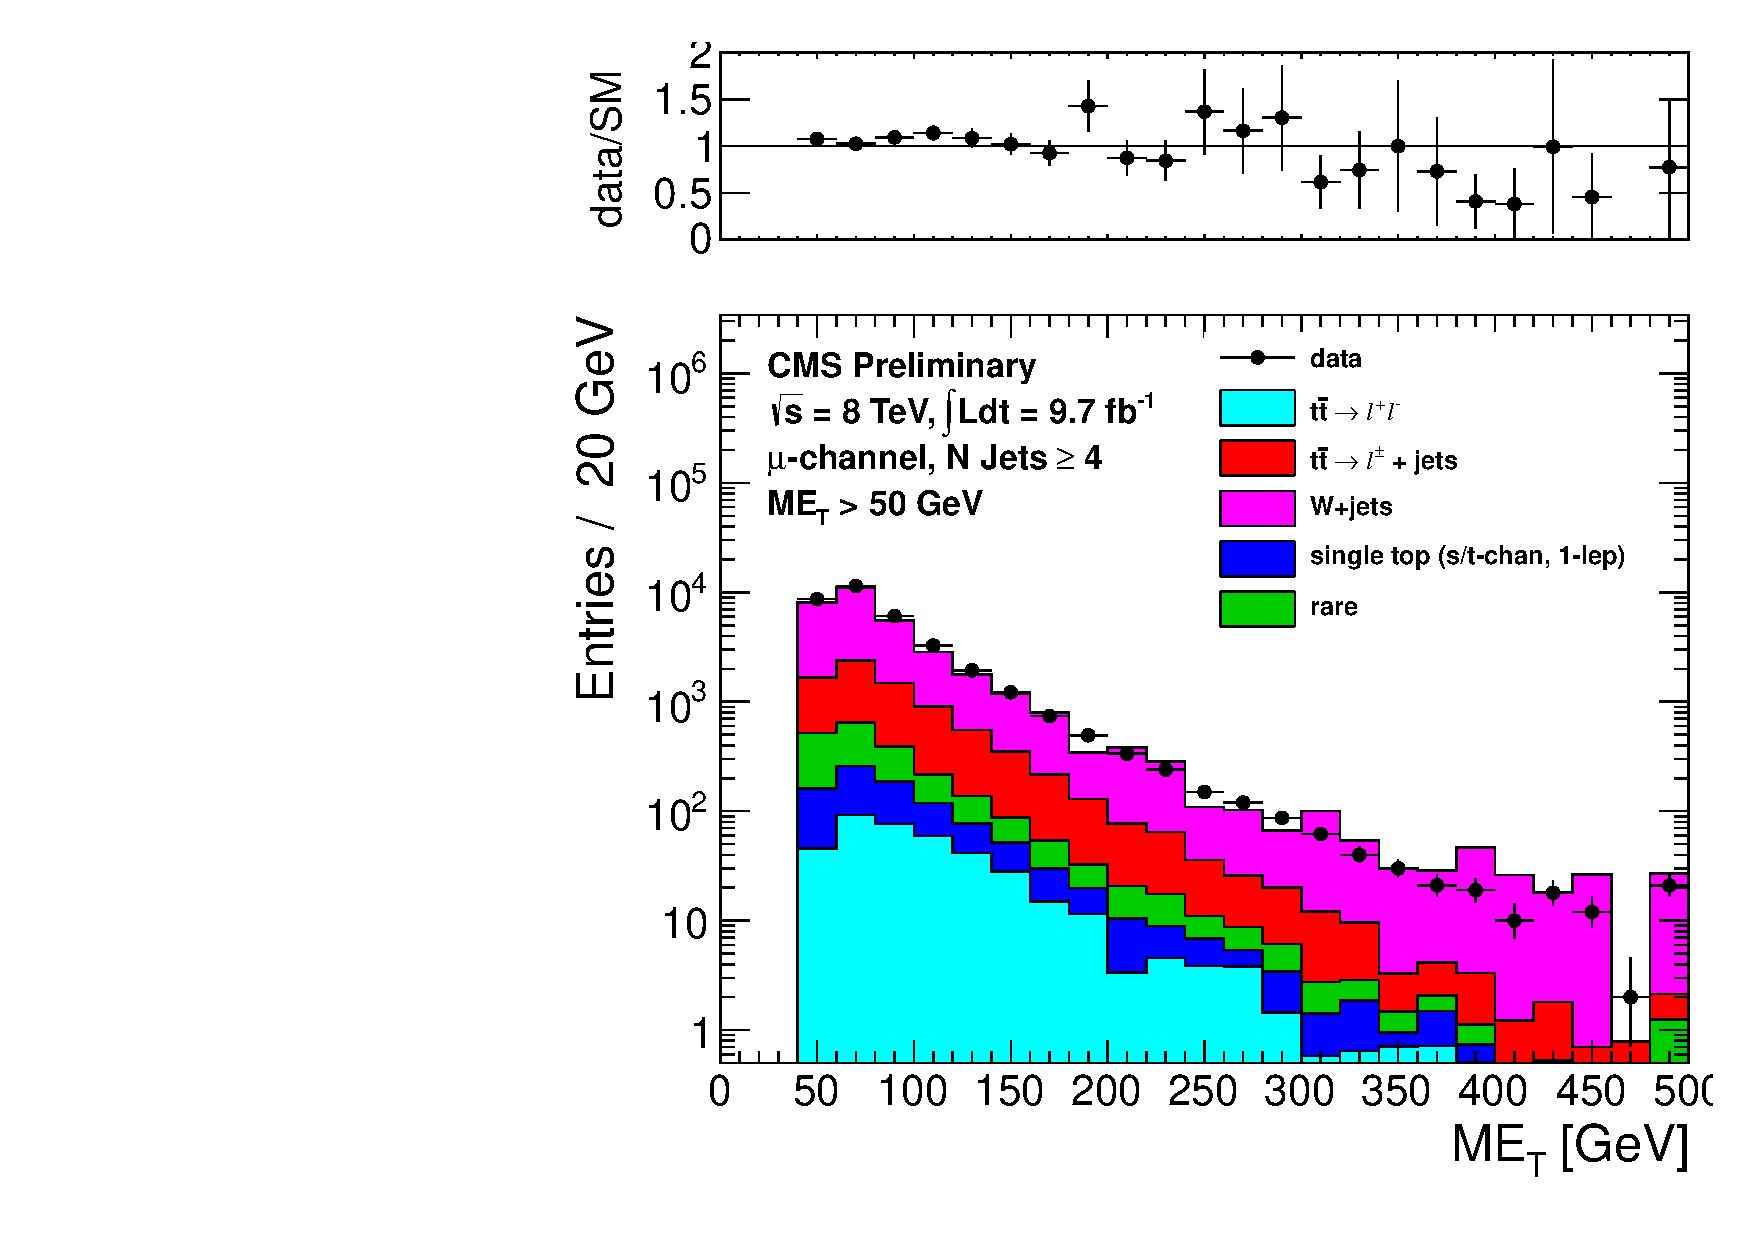
\includegraphics[width=0.5\linewidth]{plots/CR1plots/met_met50_leadmuo_nj4.pdf}%
        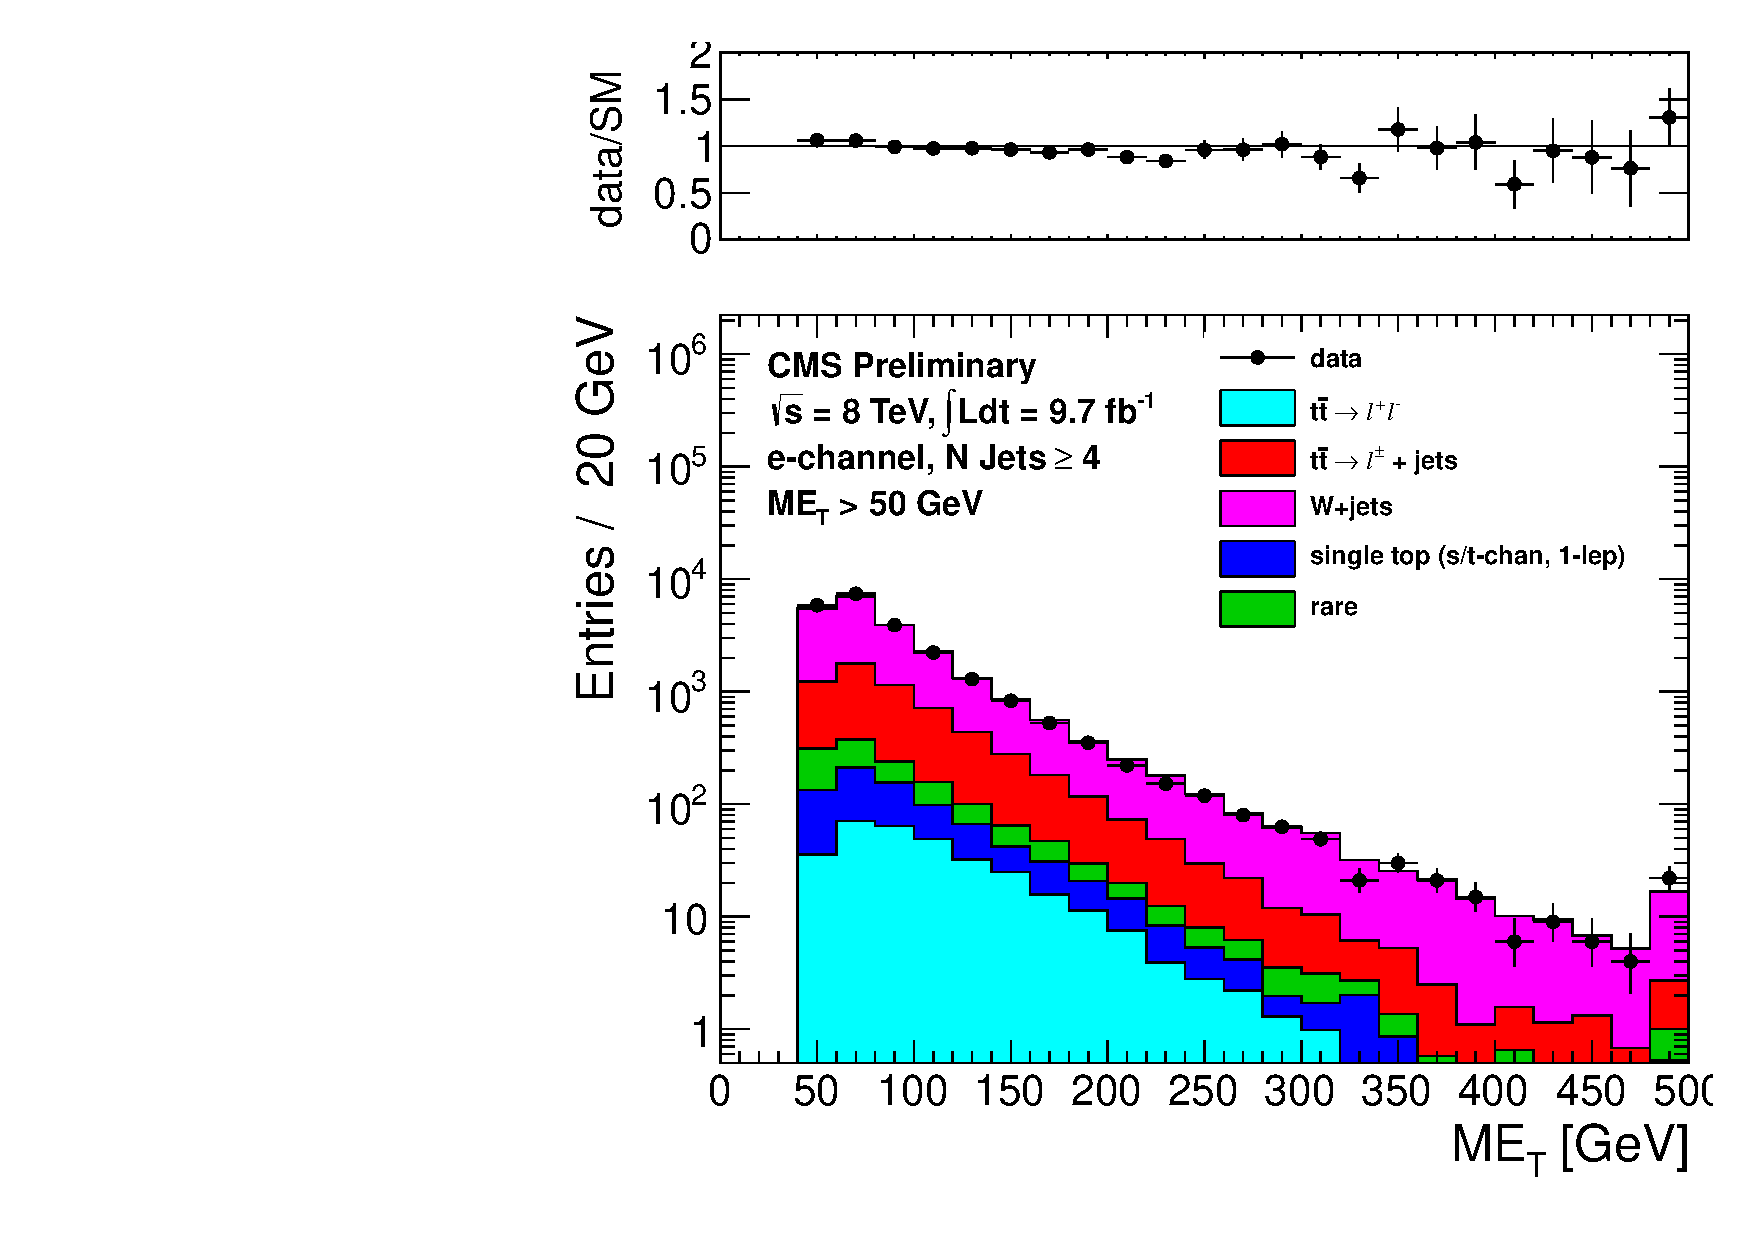
\includegraphics[width=0.5\linewidth]{plots/CR1plots/met_met50_leadele_nj4.pdf}
        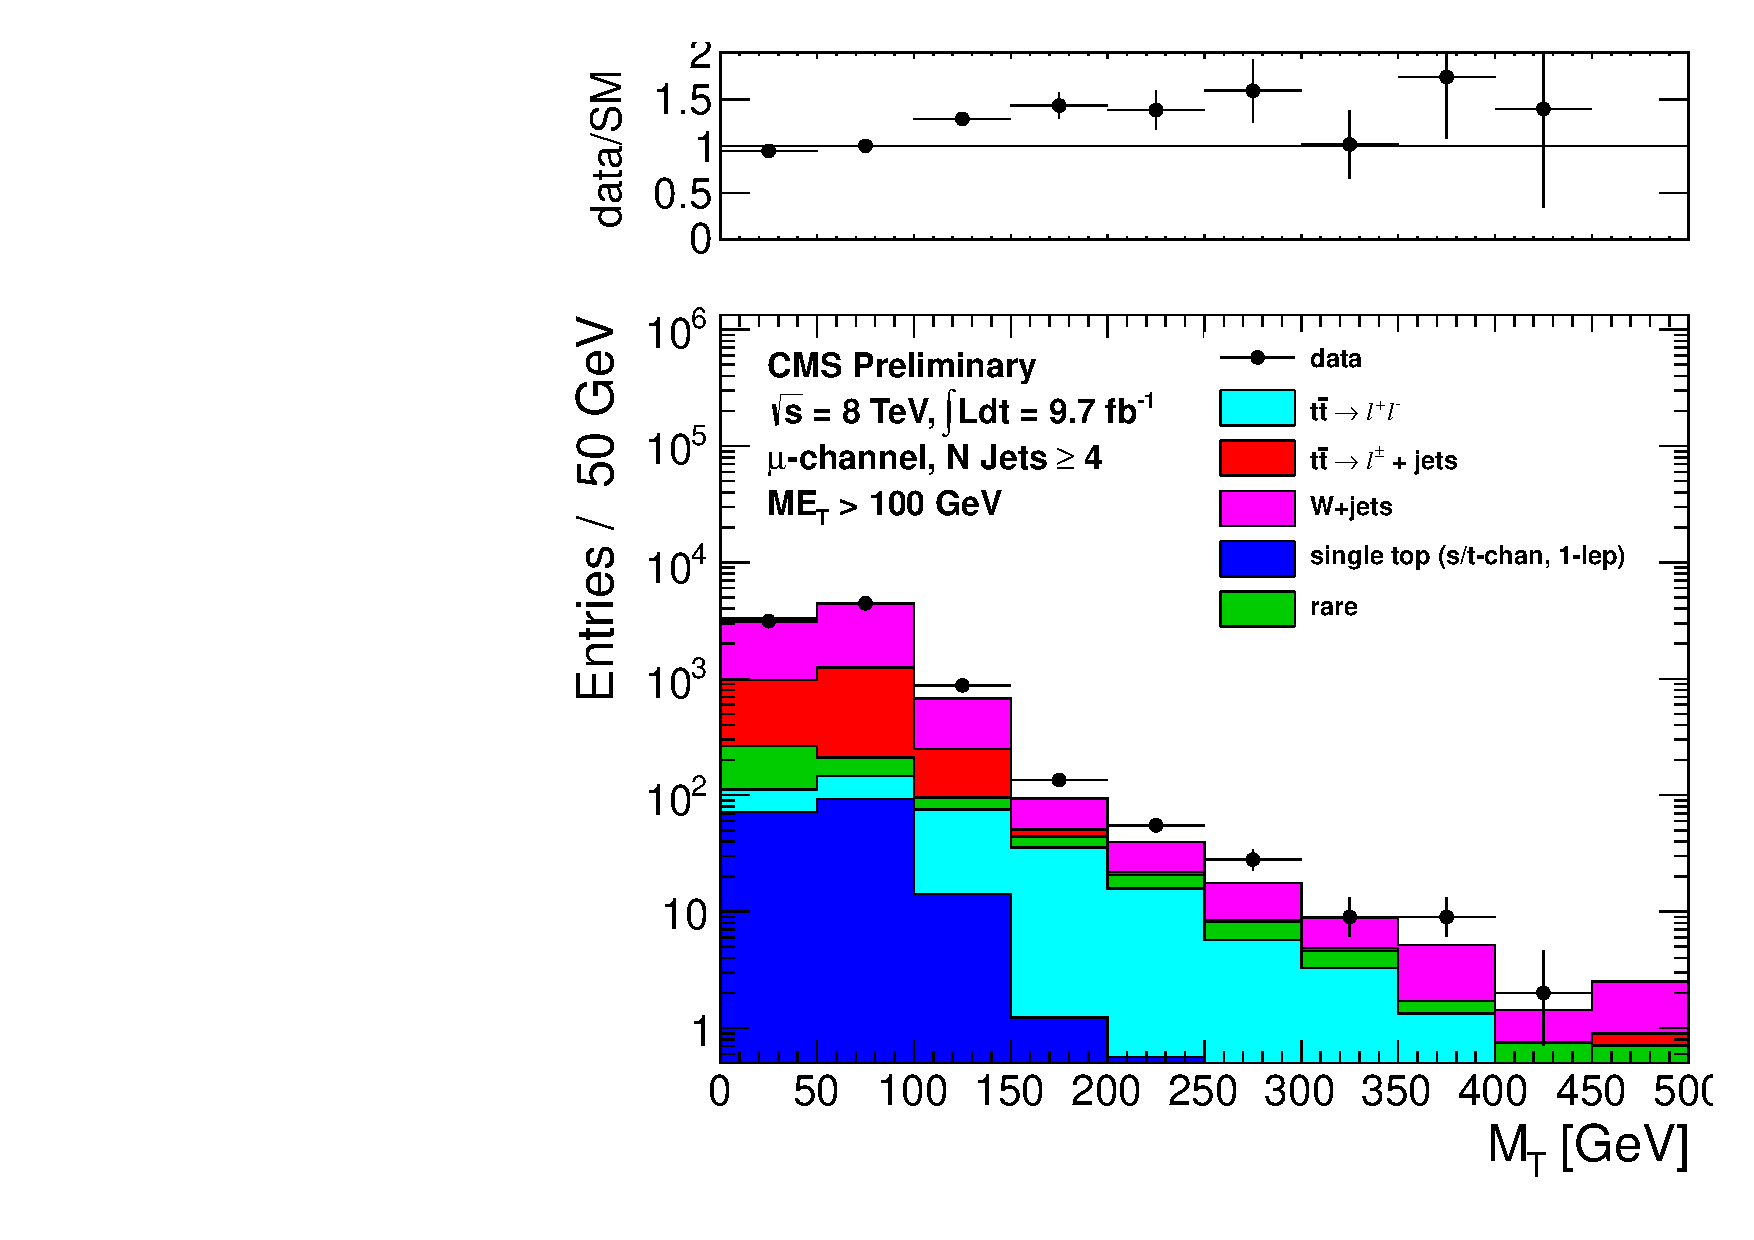
\includegraphics[width=0.5\linewidth]{plots/CR1plots/mt_met100_leadmuo_nj4.pdf}%
        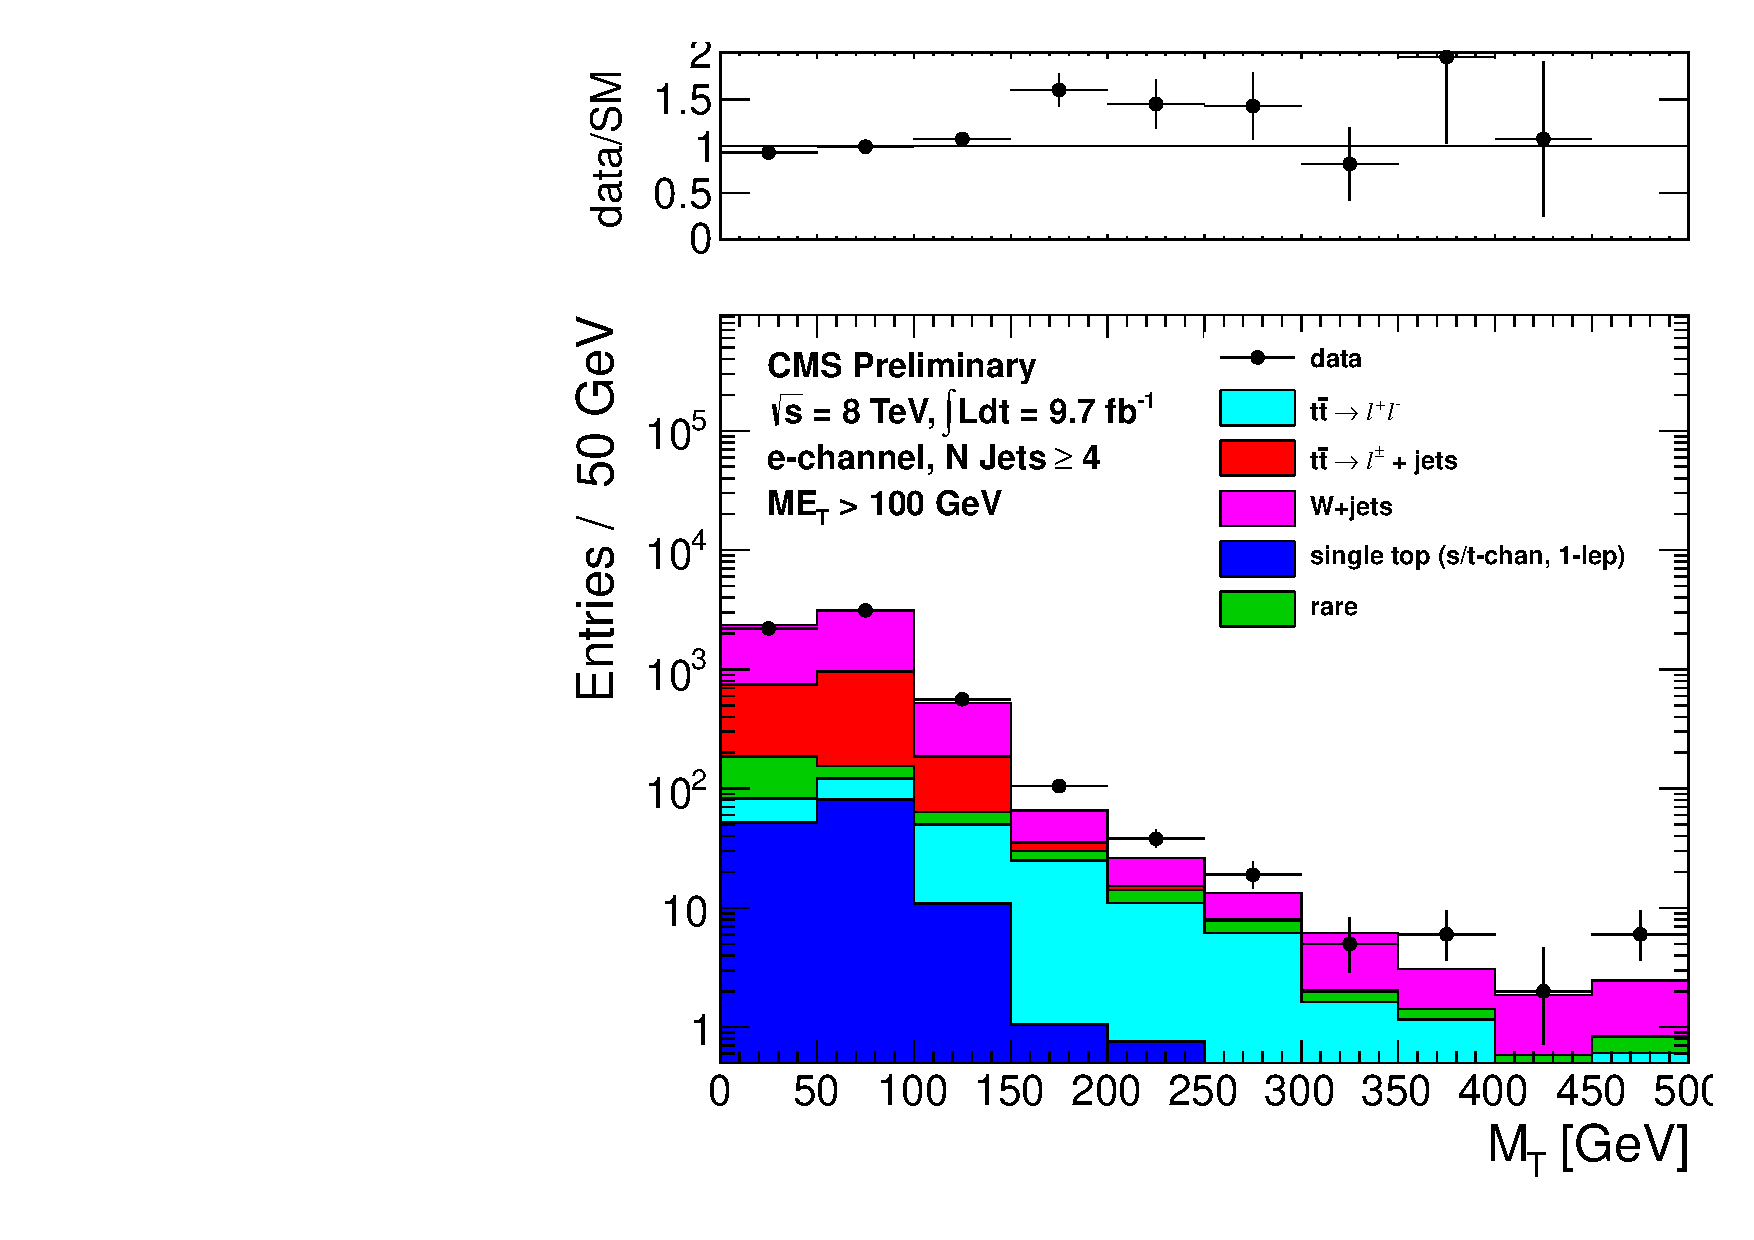
\includegraphics[width=0.5\linewidth]{plots/CR1plots/mt_met100_leadele_nj4.pdf}
    \caption{
      Comparison of the \met\ (top) and \mt\ for $\met>100$ (bottom) distributions in data vs. MC for events
      with a leading muon (left) and leading electron (right)
      satisfying the requirements of CR1. 
\label{fig:cr1met} 
}  
      \end{center}
\end{figure}


\begin{figure}[hbt]
  \begin{center}
        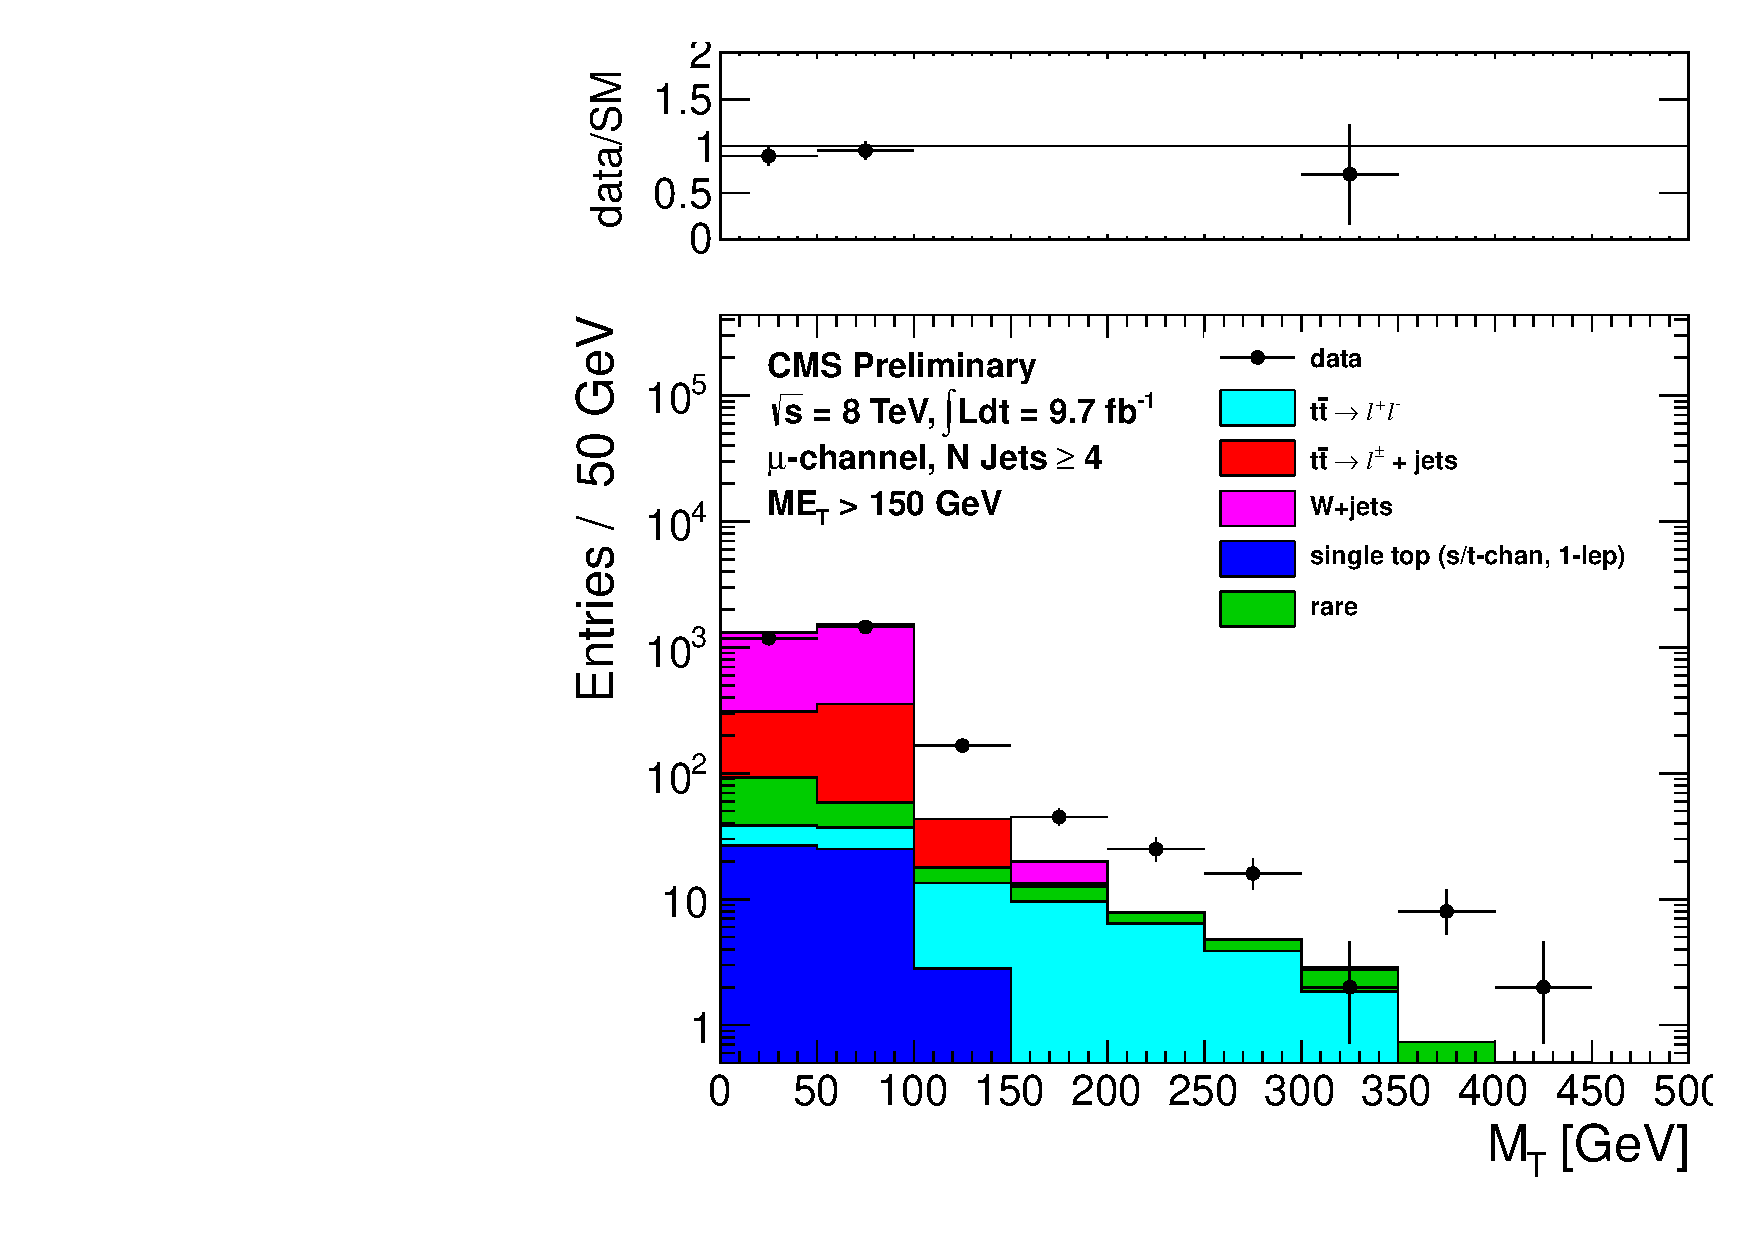
\includegraphics[width=0.5\linewidth]{plots/CR1plots/mt_met150_leadmuo_nj4.pdf}%
        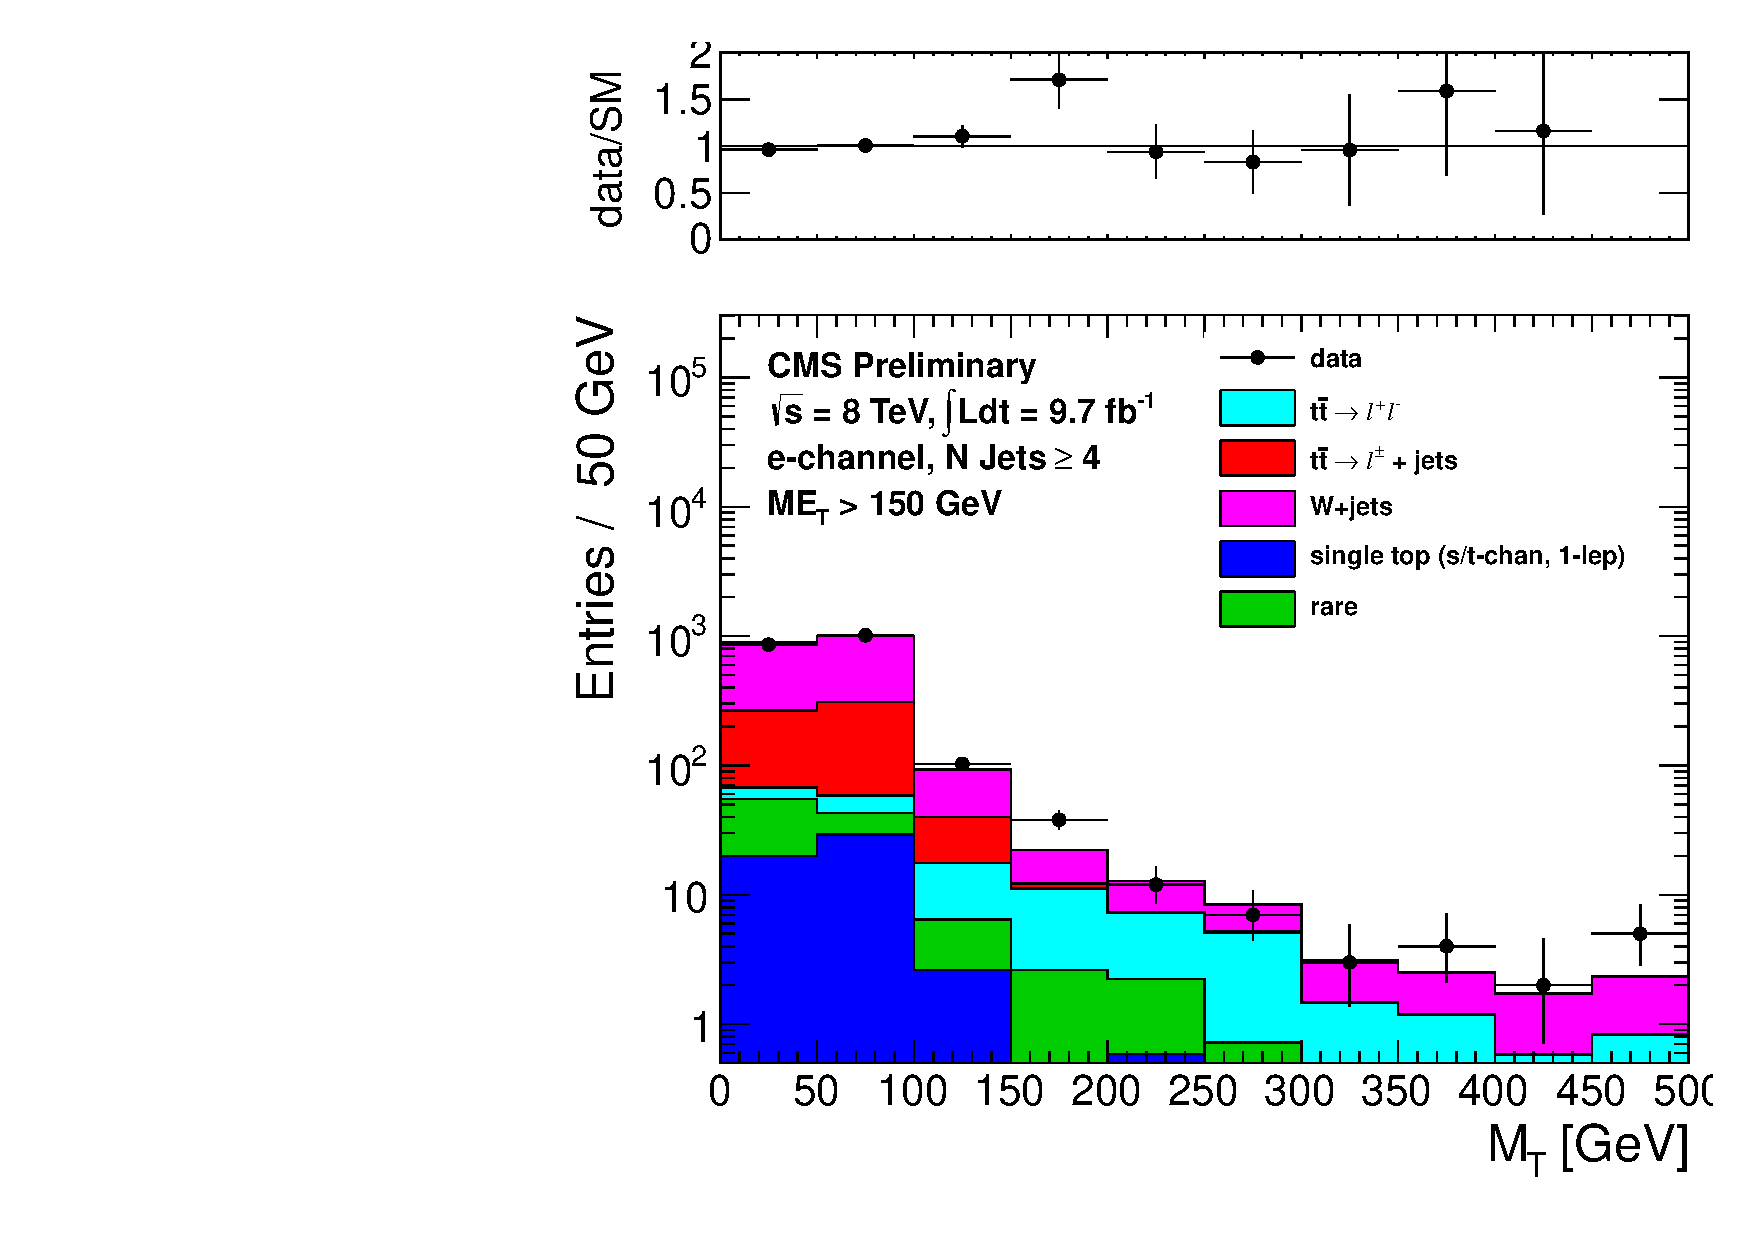
\includegraphics[width=0.5\linewidth]{plots/CR1plots/mt_met150_leadele_nj4.pdf}
        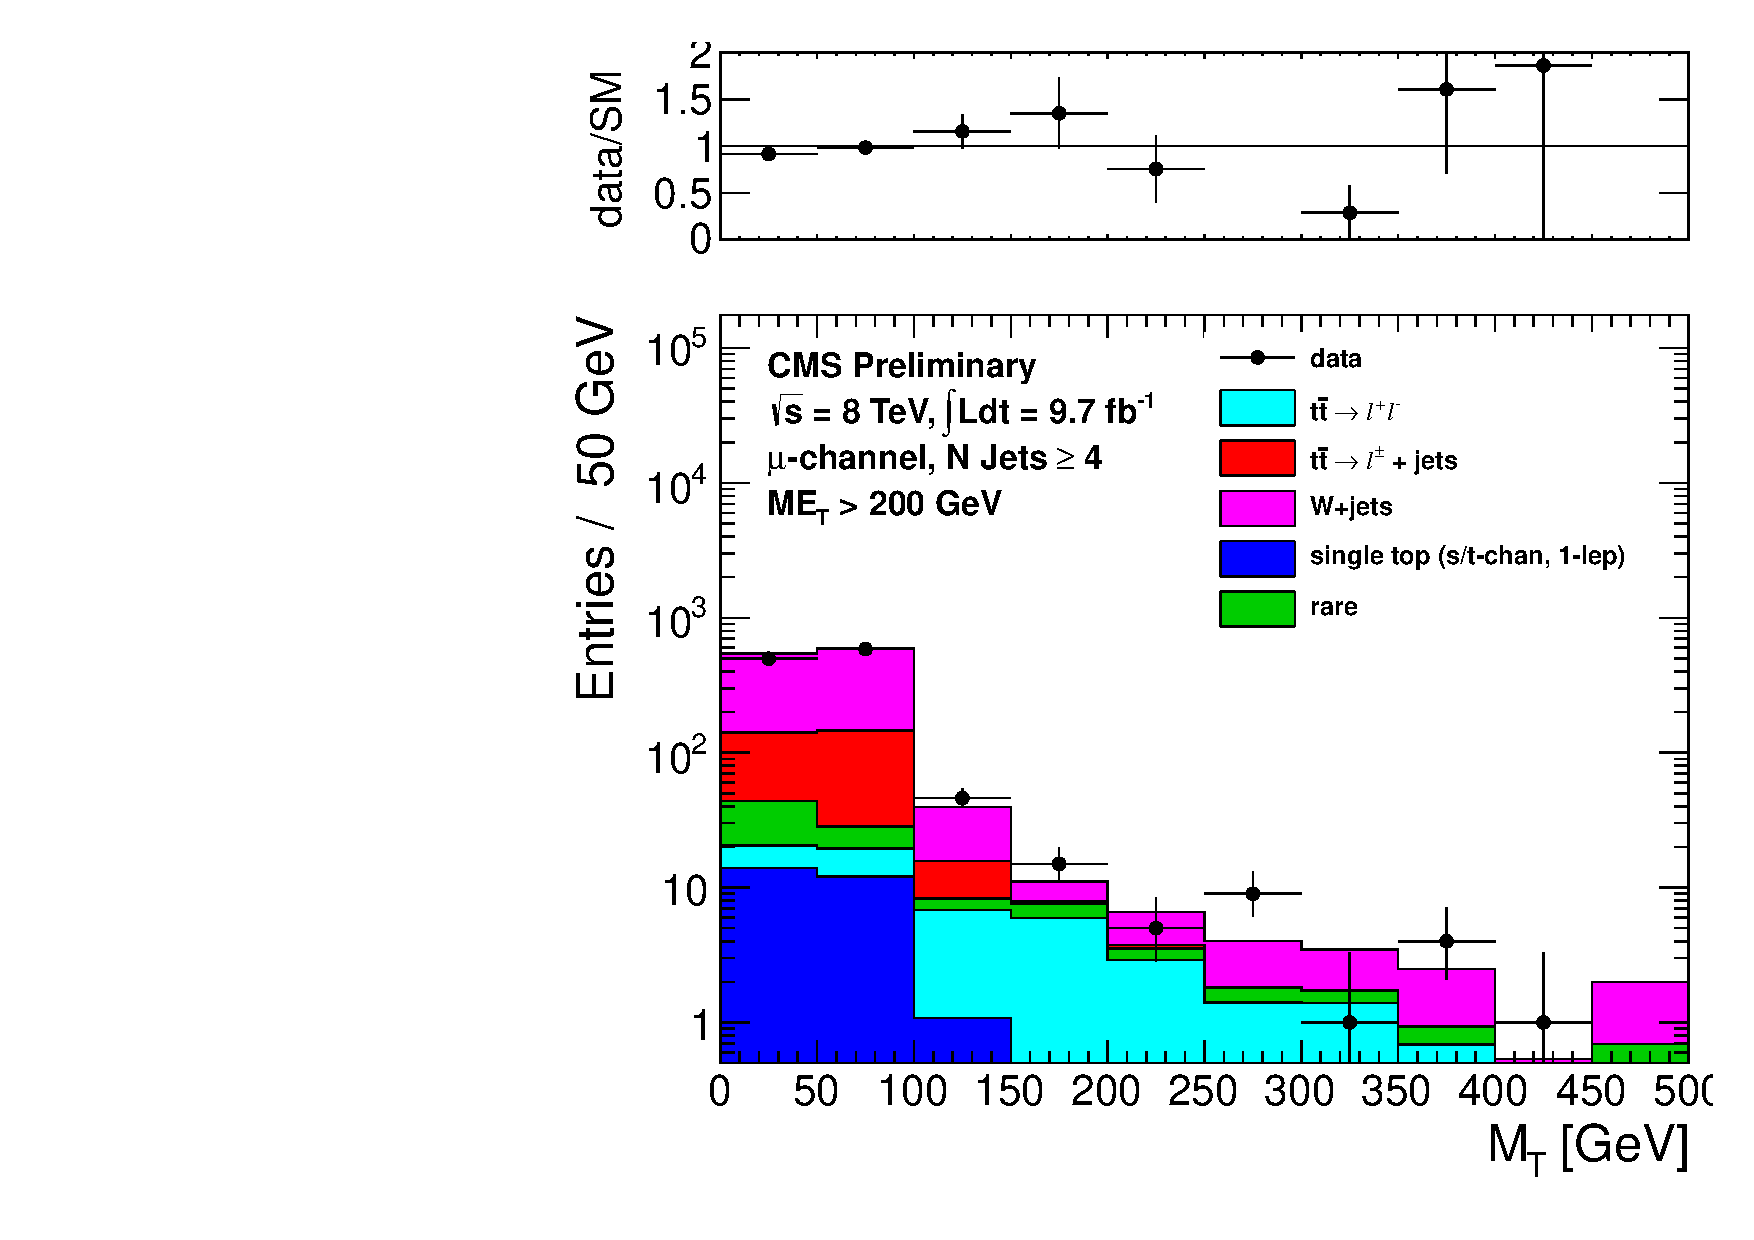
\includegraphics[width=0.5\linewidth]{plots/CR1plots/mt_met200_leadmuo_nj4.pdf}%
        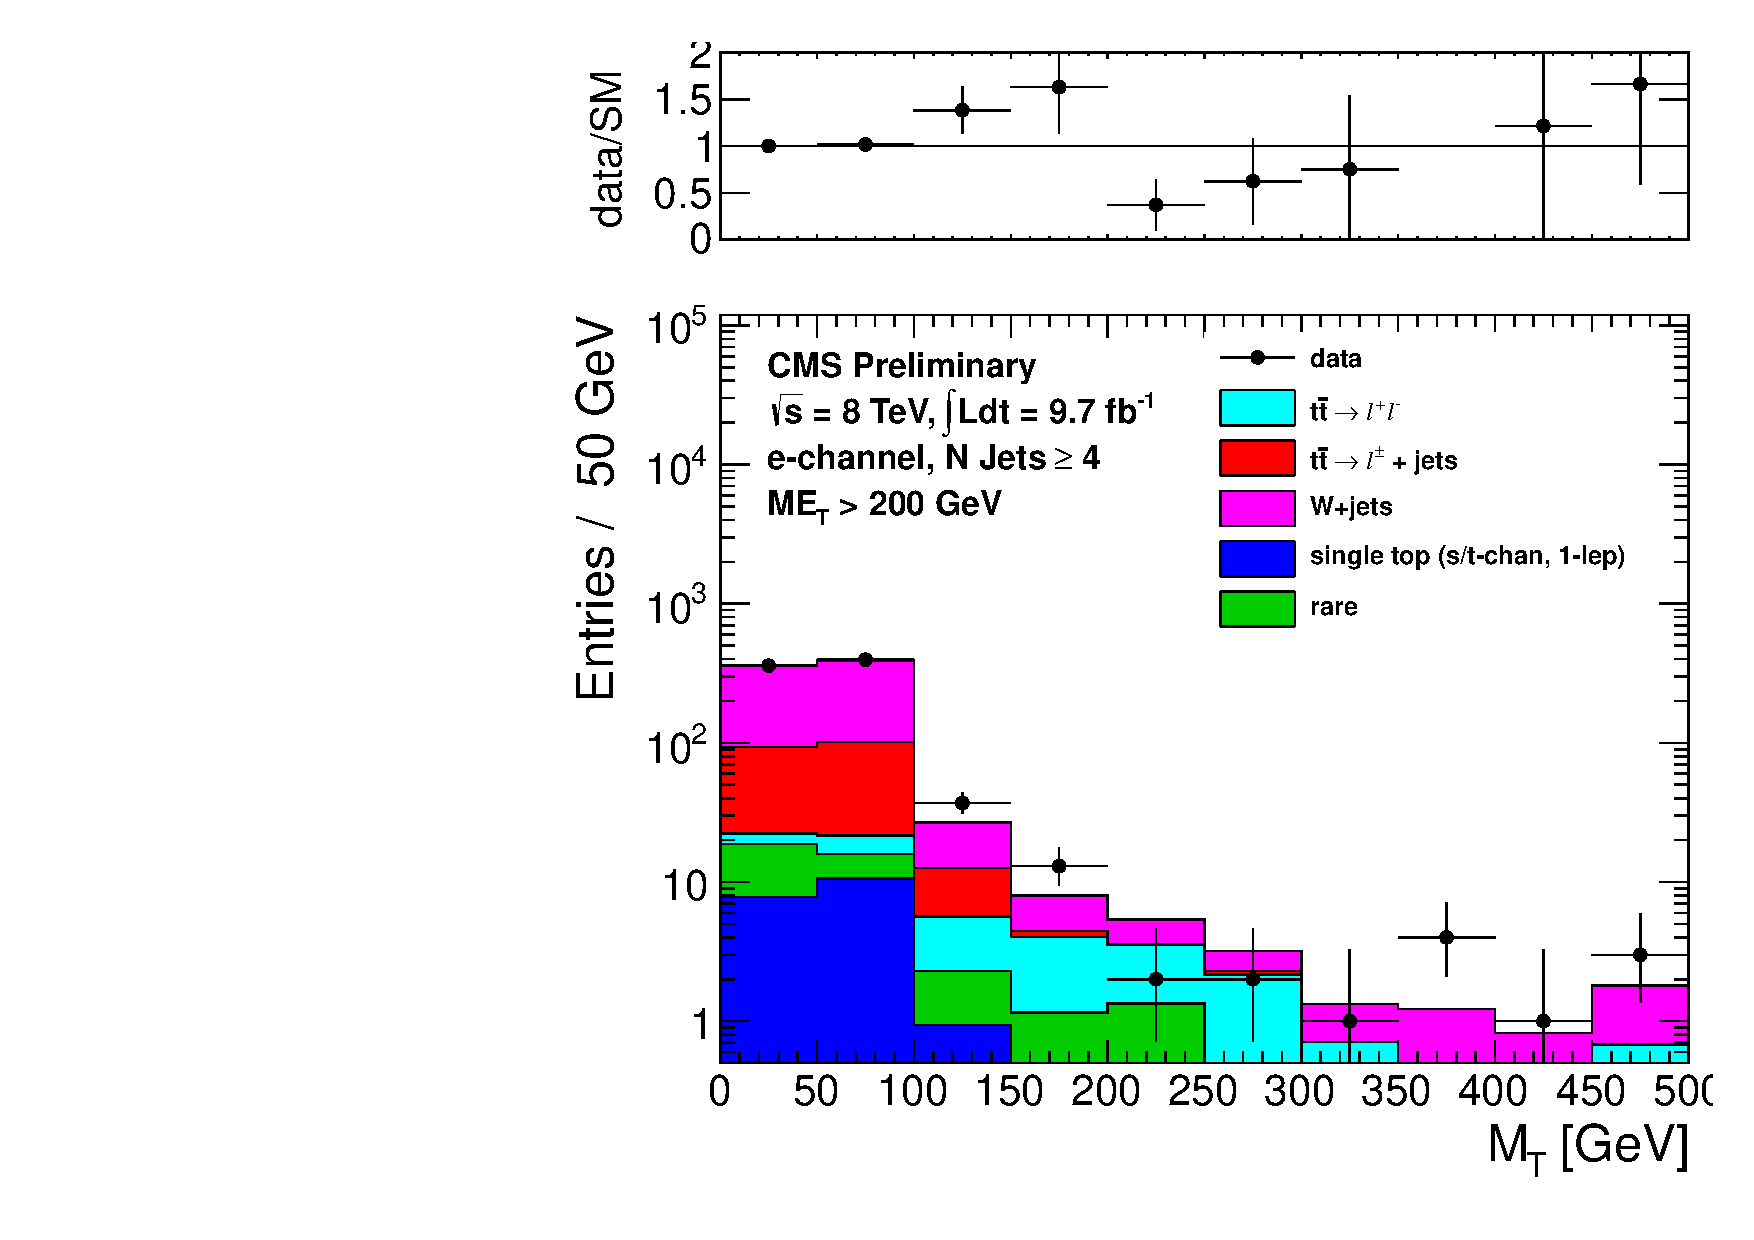
\includegraphics[width=0.5\linewidth]{plots/CR1plots/mt_met200_leadele_nj4.pdf}
        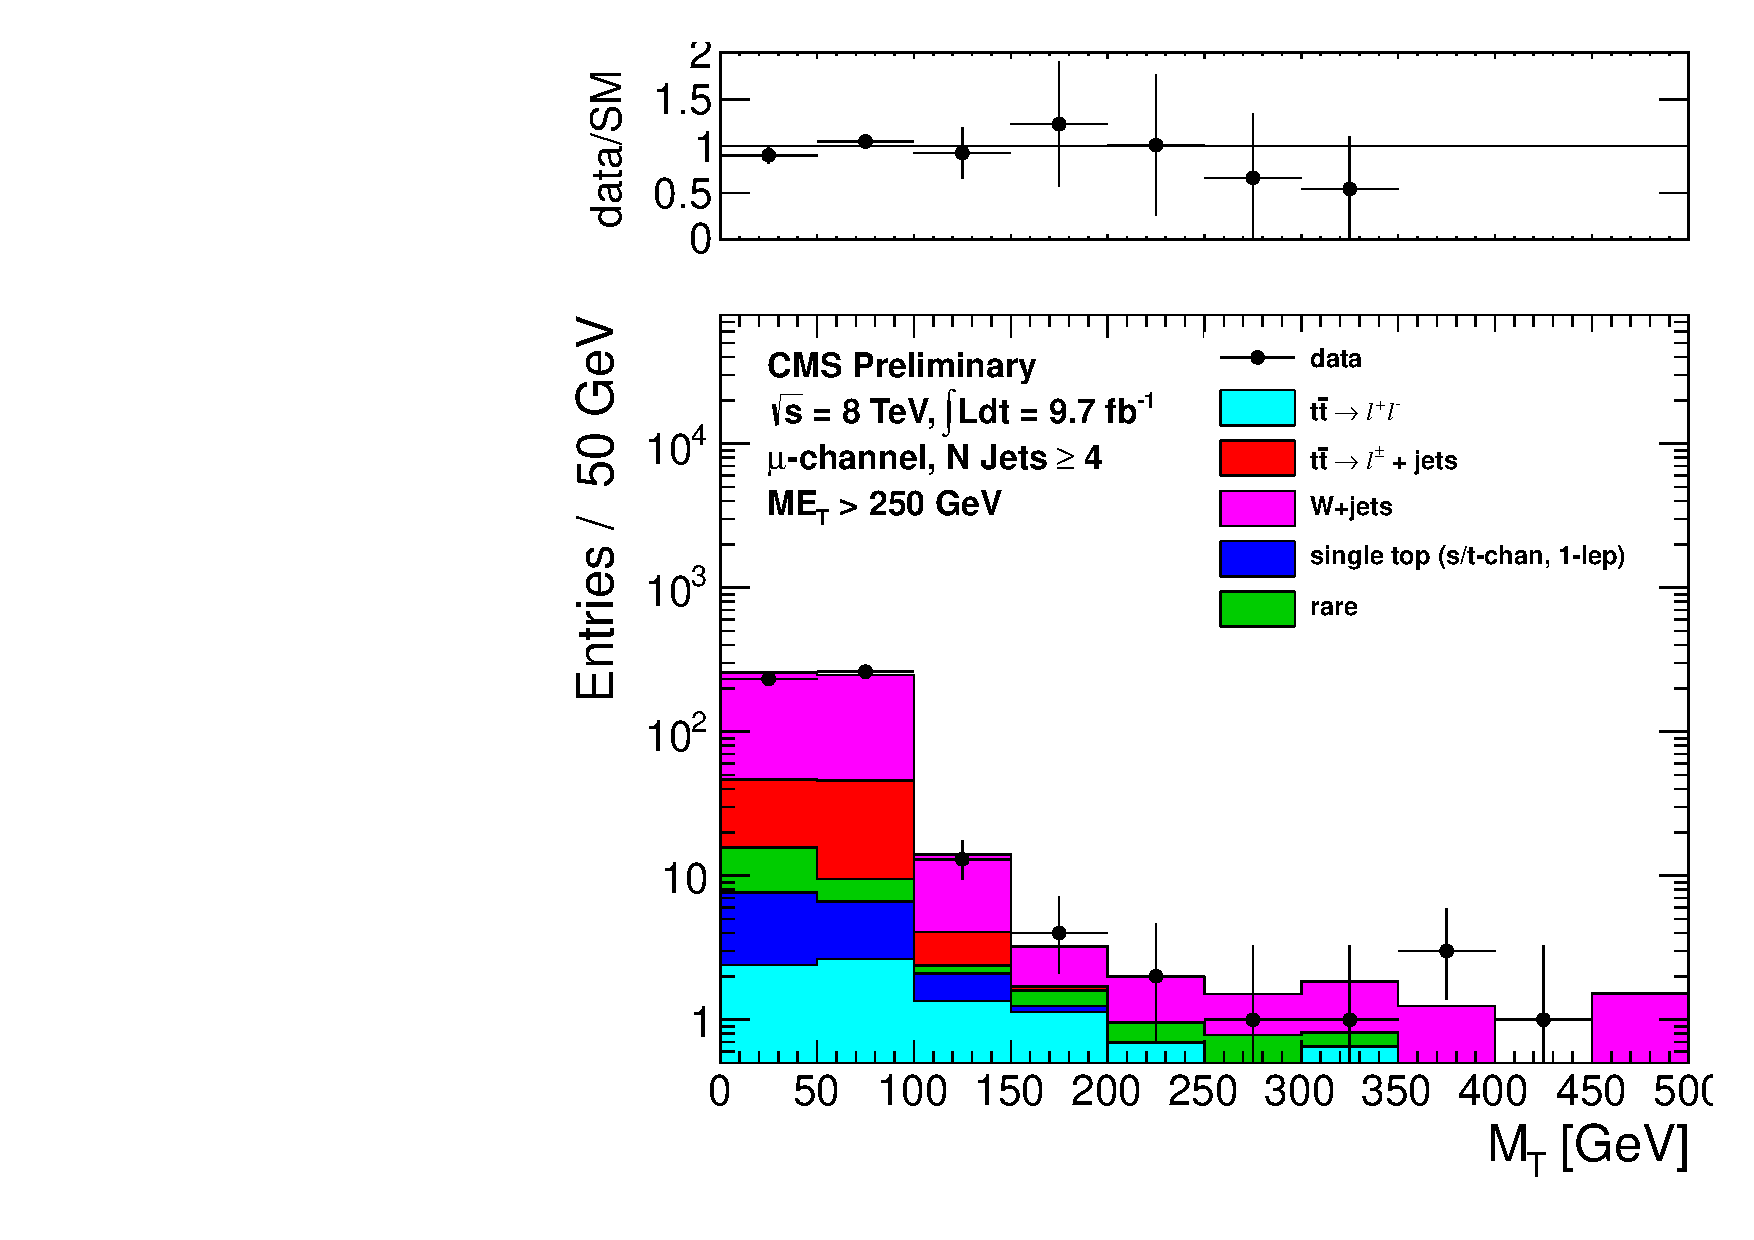
\includegraphics[width=0.5\linewidth]{plots/CR1plots/mt_met250_leadmuo_nj4.pdf}%
        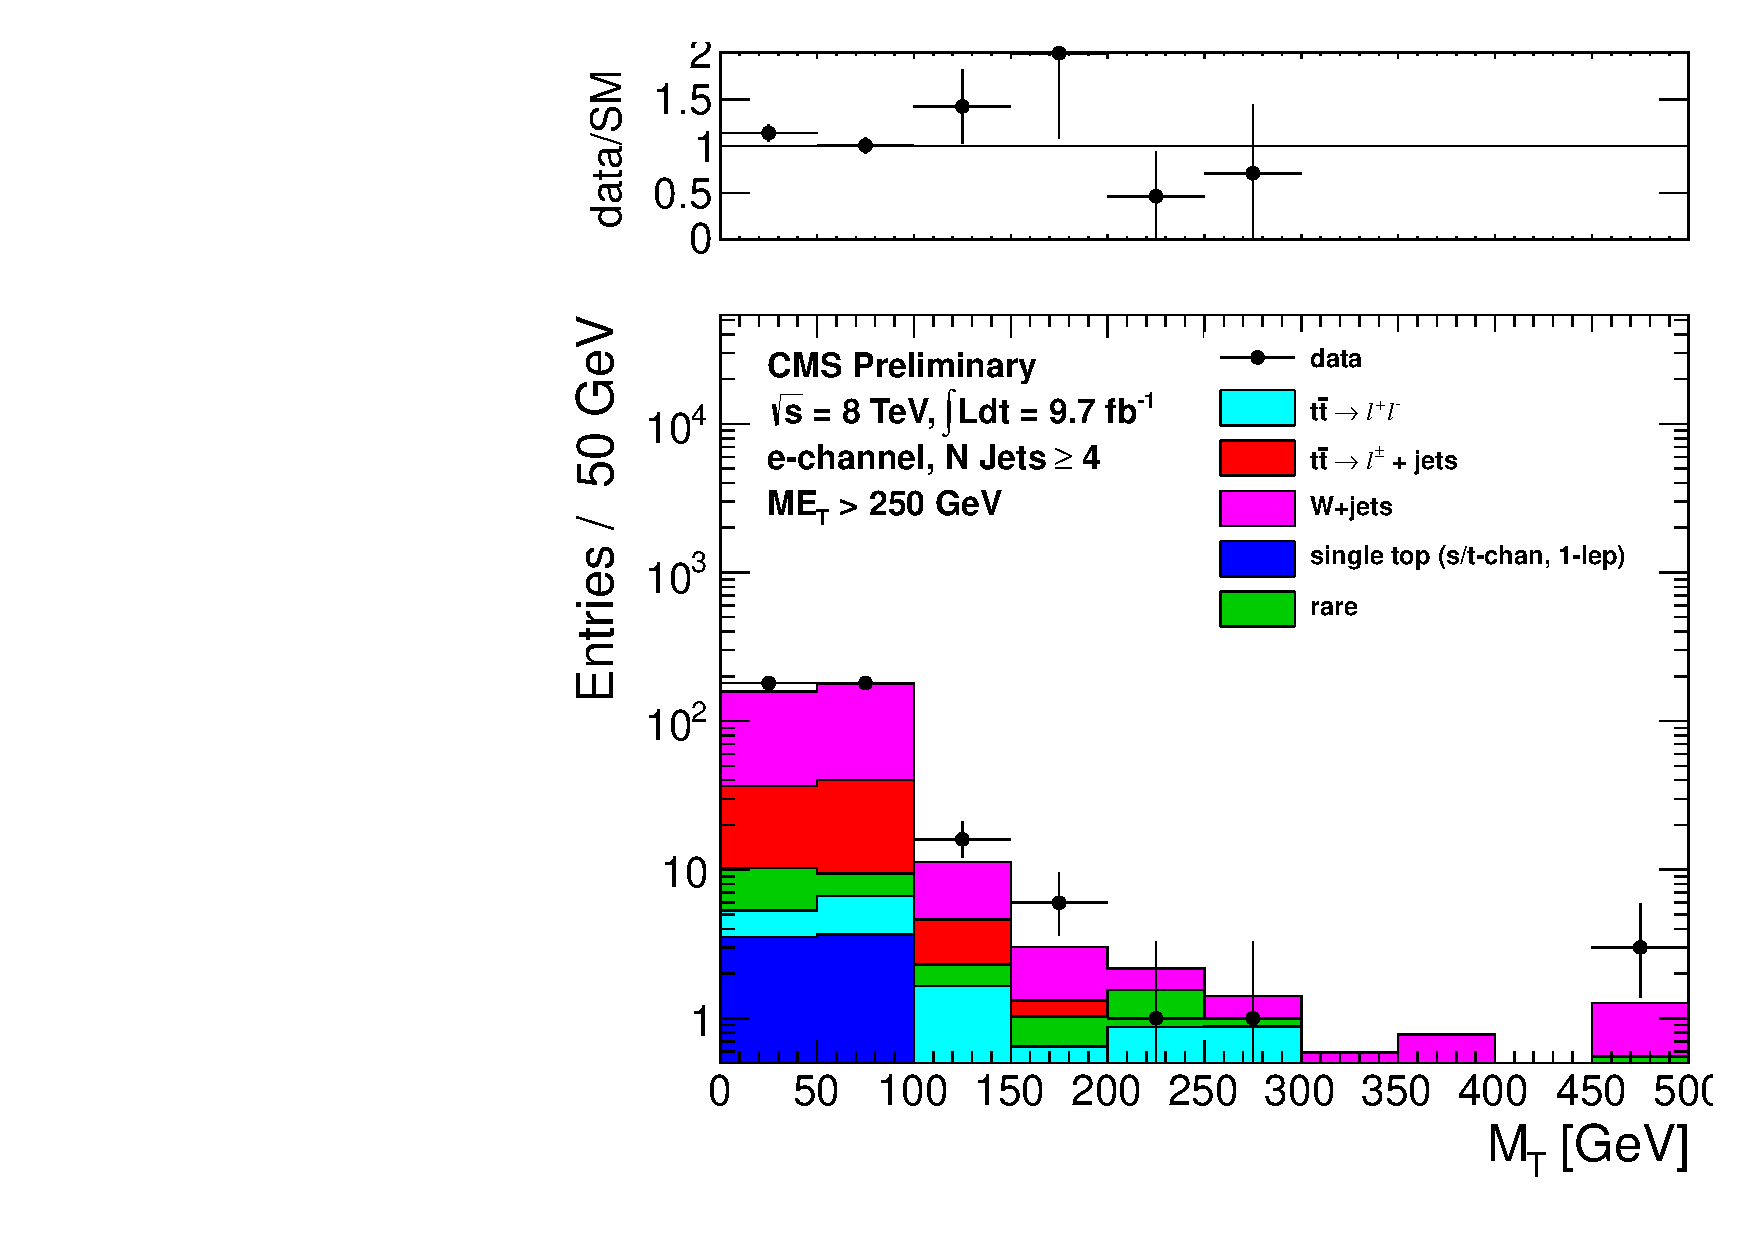
\includegraphics[width=0.5\linewidth]{plots/CR1plots/mt_met250_leadele_nj4.pdf}
    \caption{
      Comparison of the \mt\ distribution in data vs. MC for events
      with a leading muon (left) and leading electron (right)
      satisfying the requirements of CR1. The \met\ requirements used are
      150 GeV (top), 200 GeV (middle) and 250 GeV (bottom).
\label{fig:cr1mtrest} 
}  
      \end{center}
\end{figure}

\begin{figure}[hbt]
  \begin{center}
        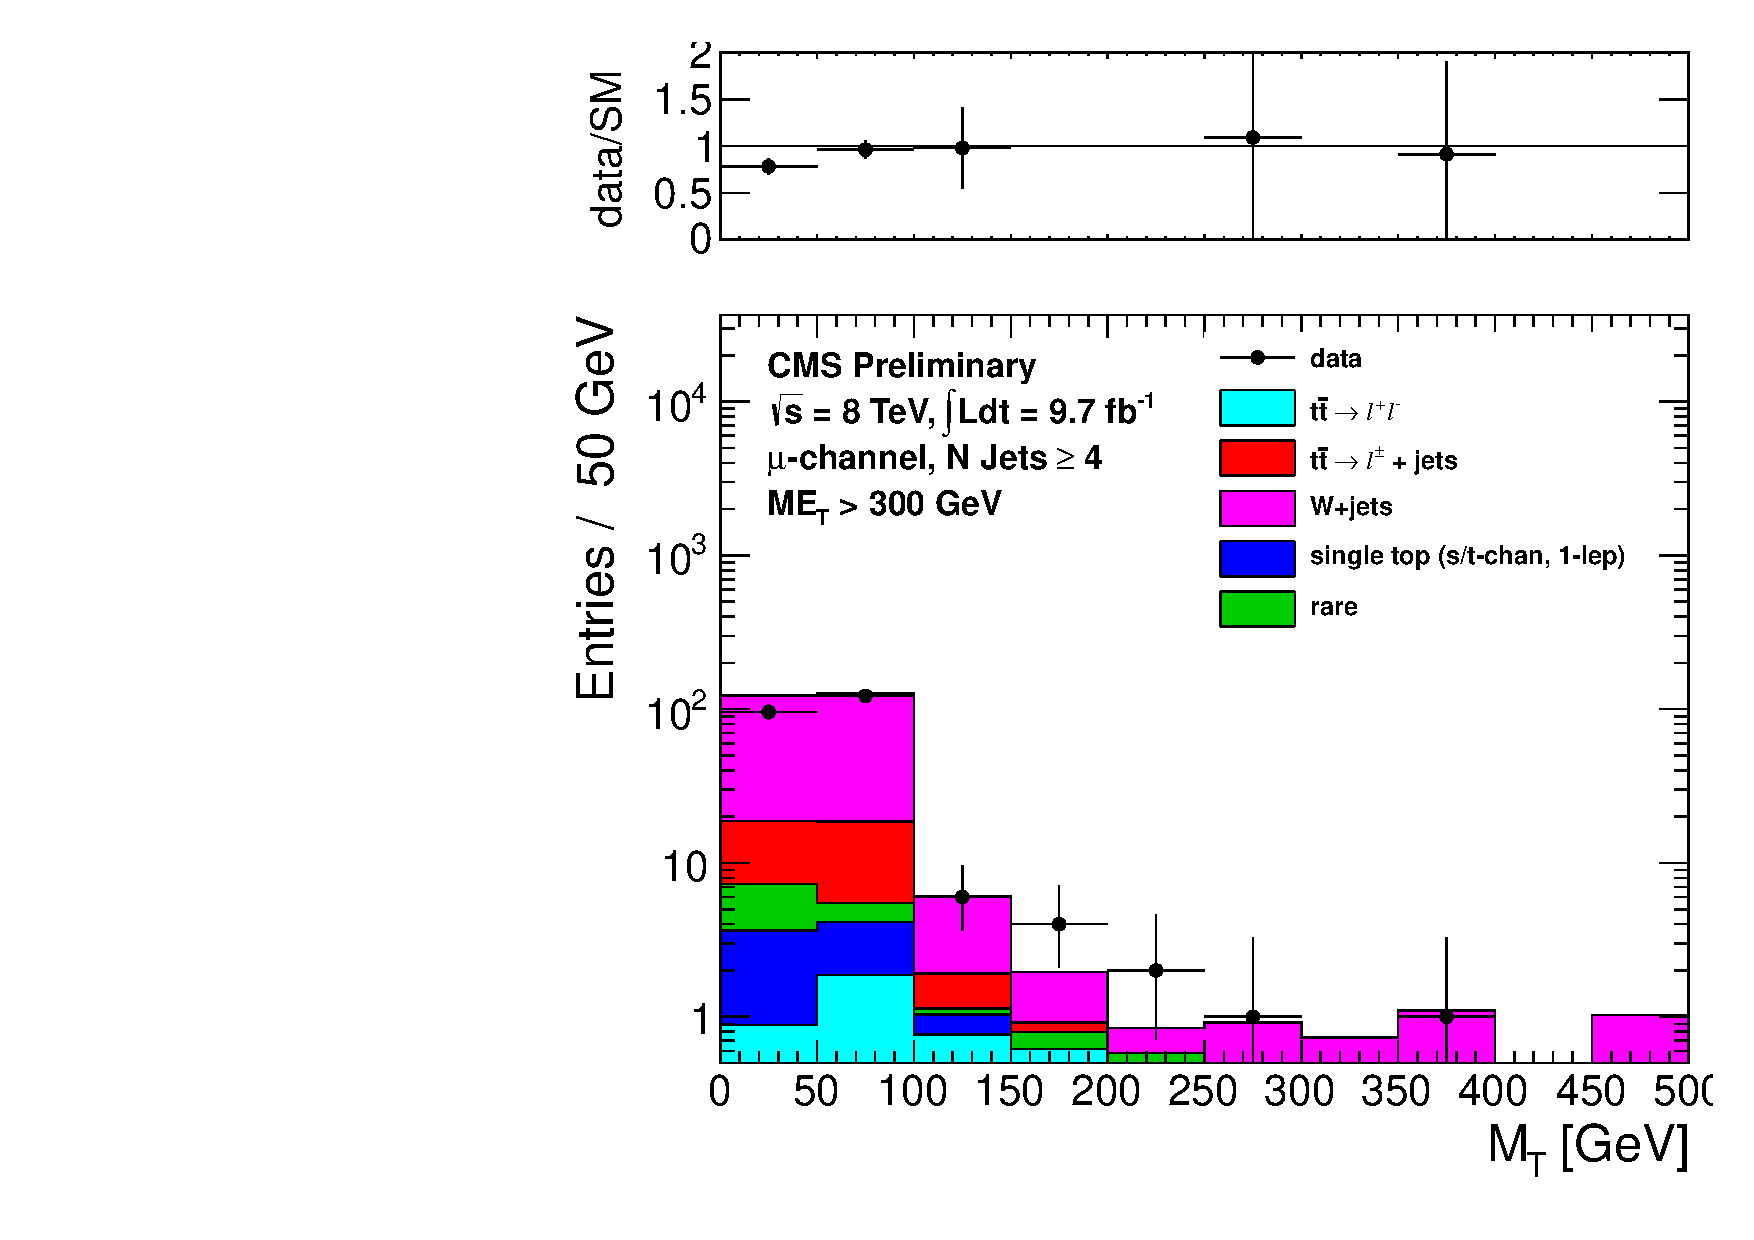
\includegraphics[width=0.5\linewidth]{plots/CR1plots/mt_met300_leadmuo_nj4.pdf}%
        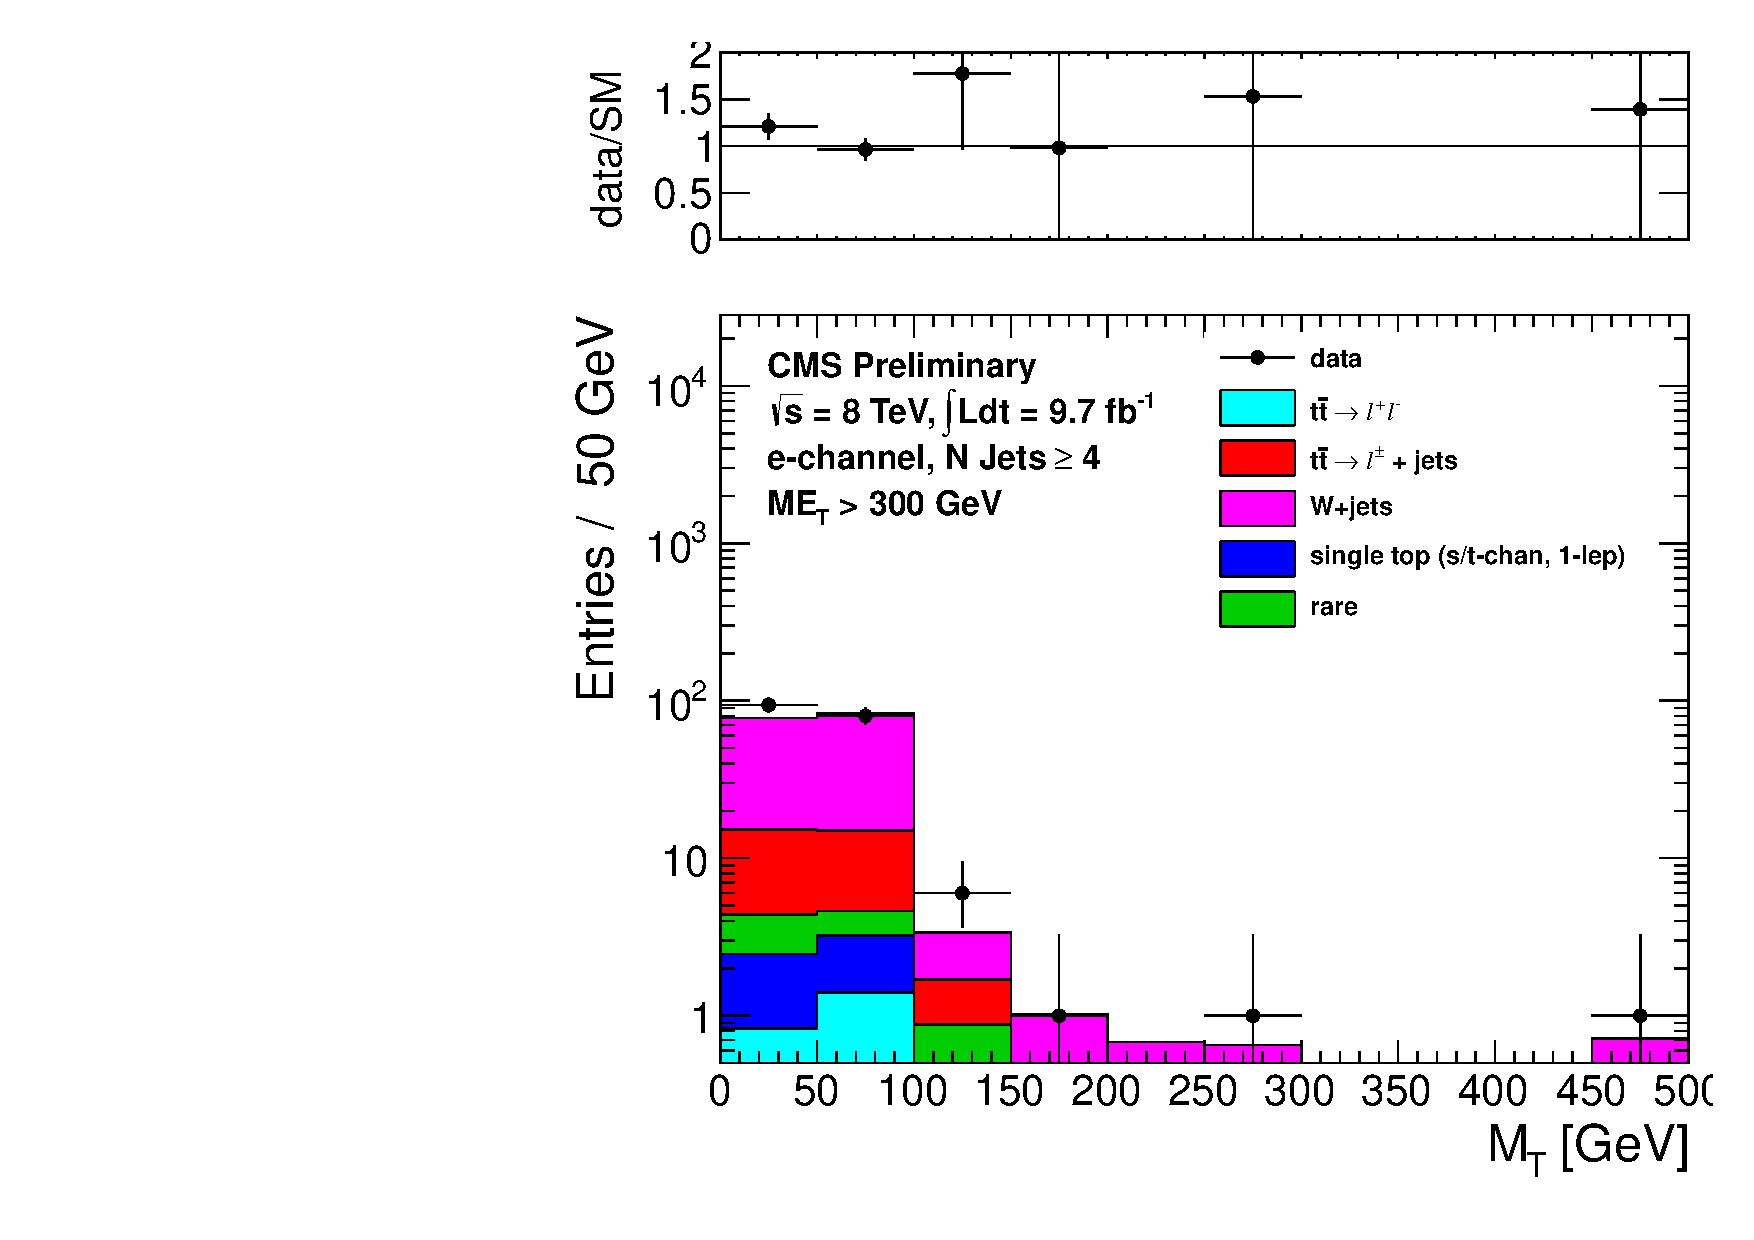
\includegraphics[width=0.5\linewidth]{plots/CR1plots/mt_met300_leadele_nj4.pdf}
        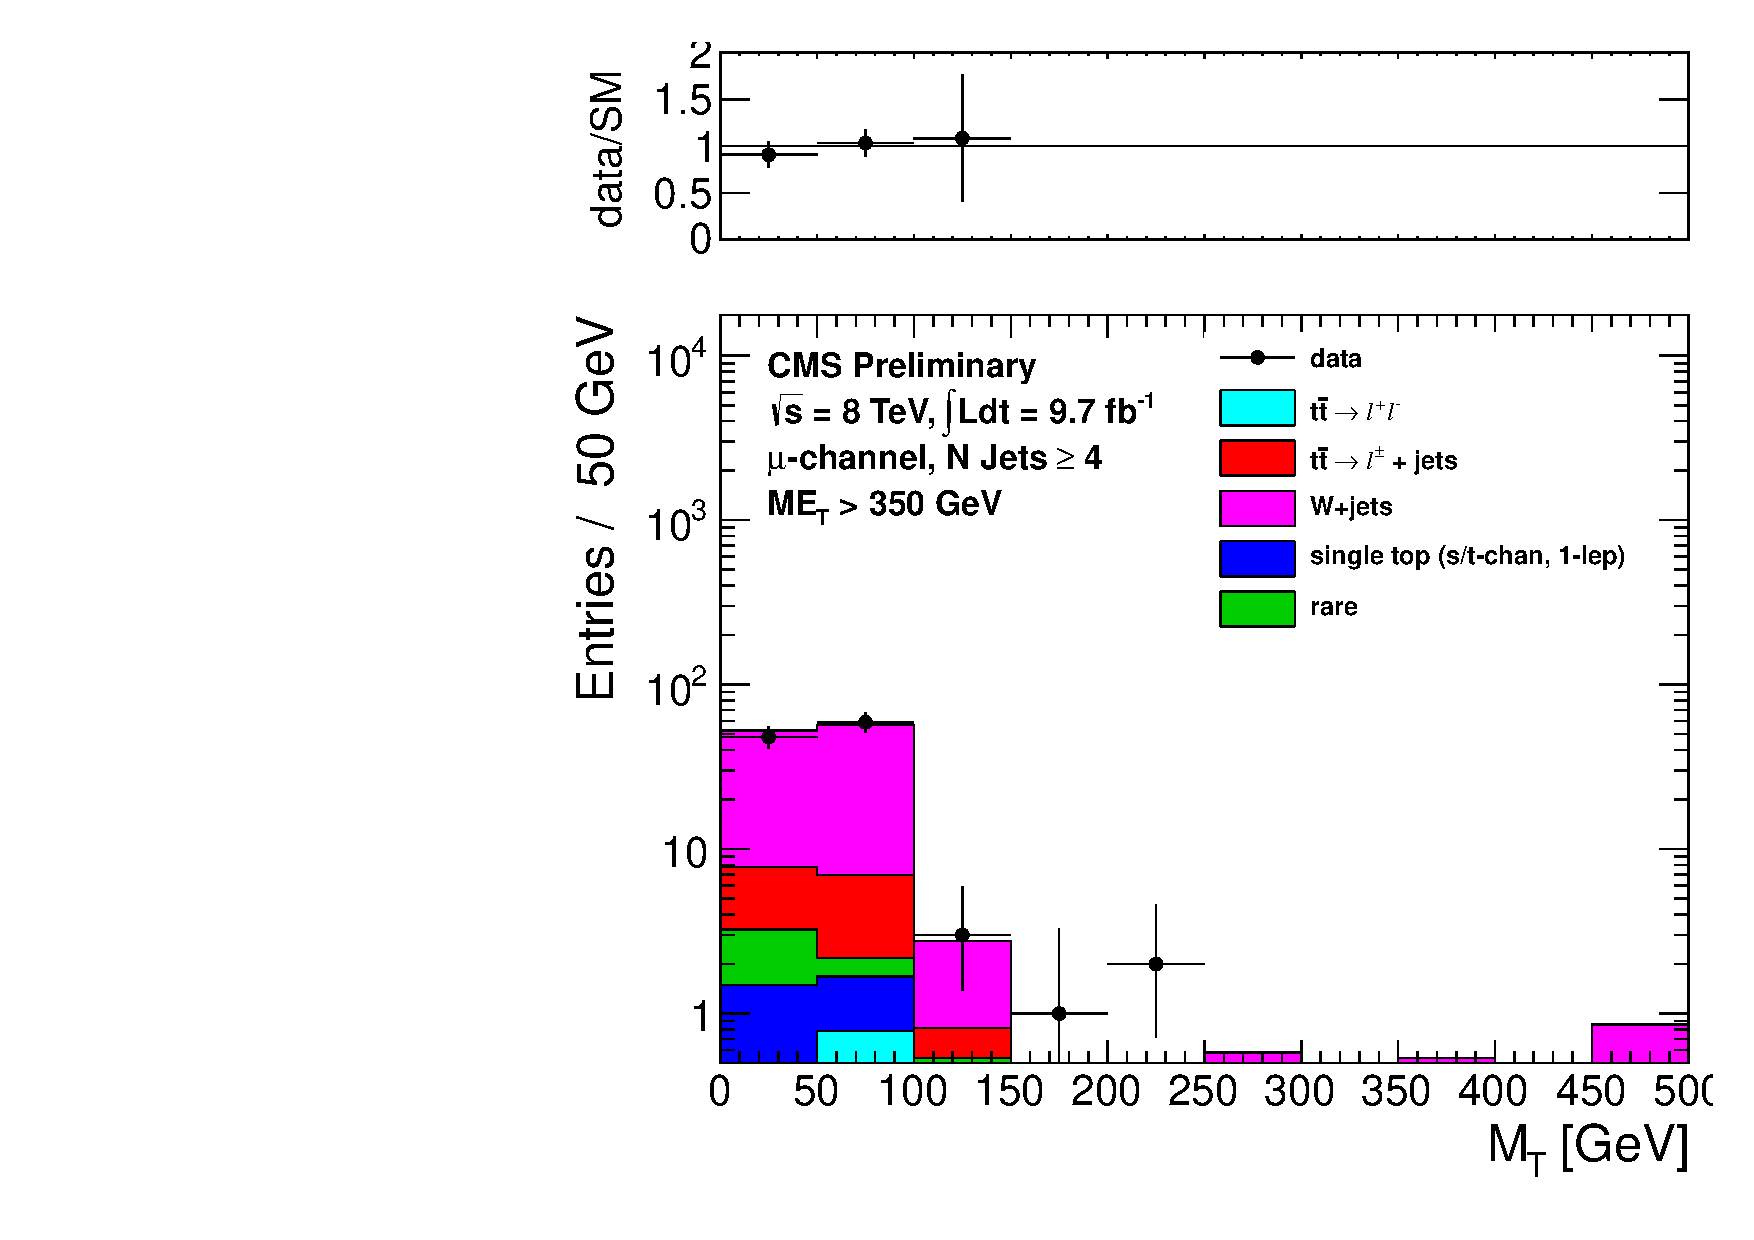
\includegraphics[width=0.5\linewidth]{plots/CR1plots/mt_met350_leadmuo_nj4.pdf}%
        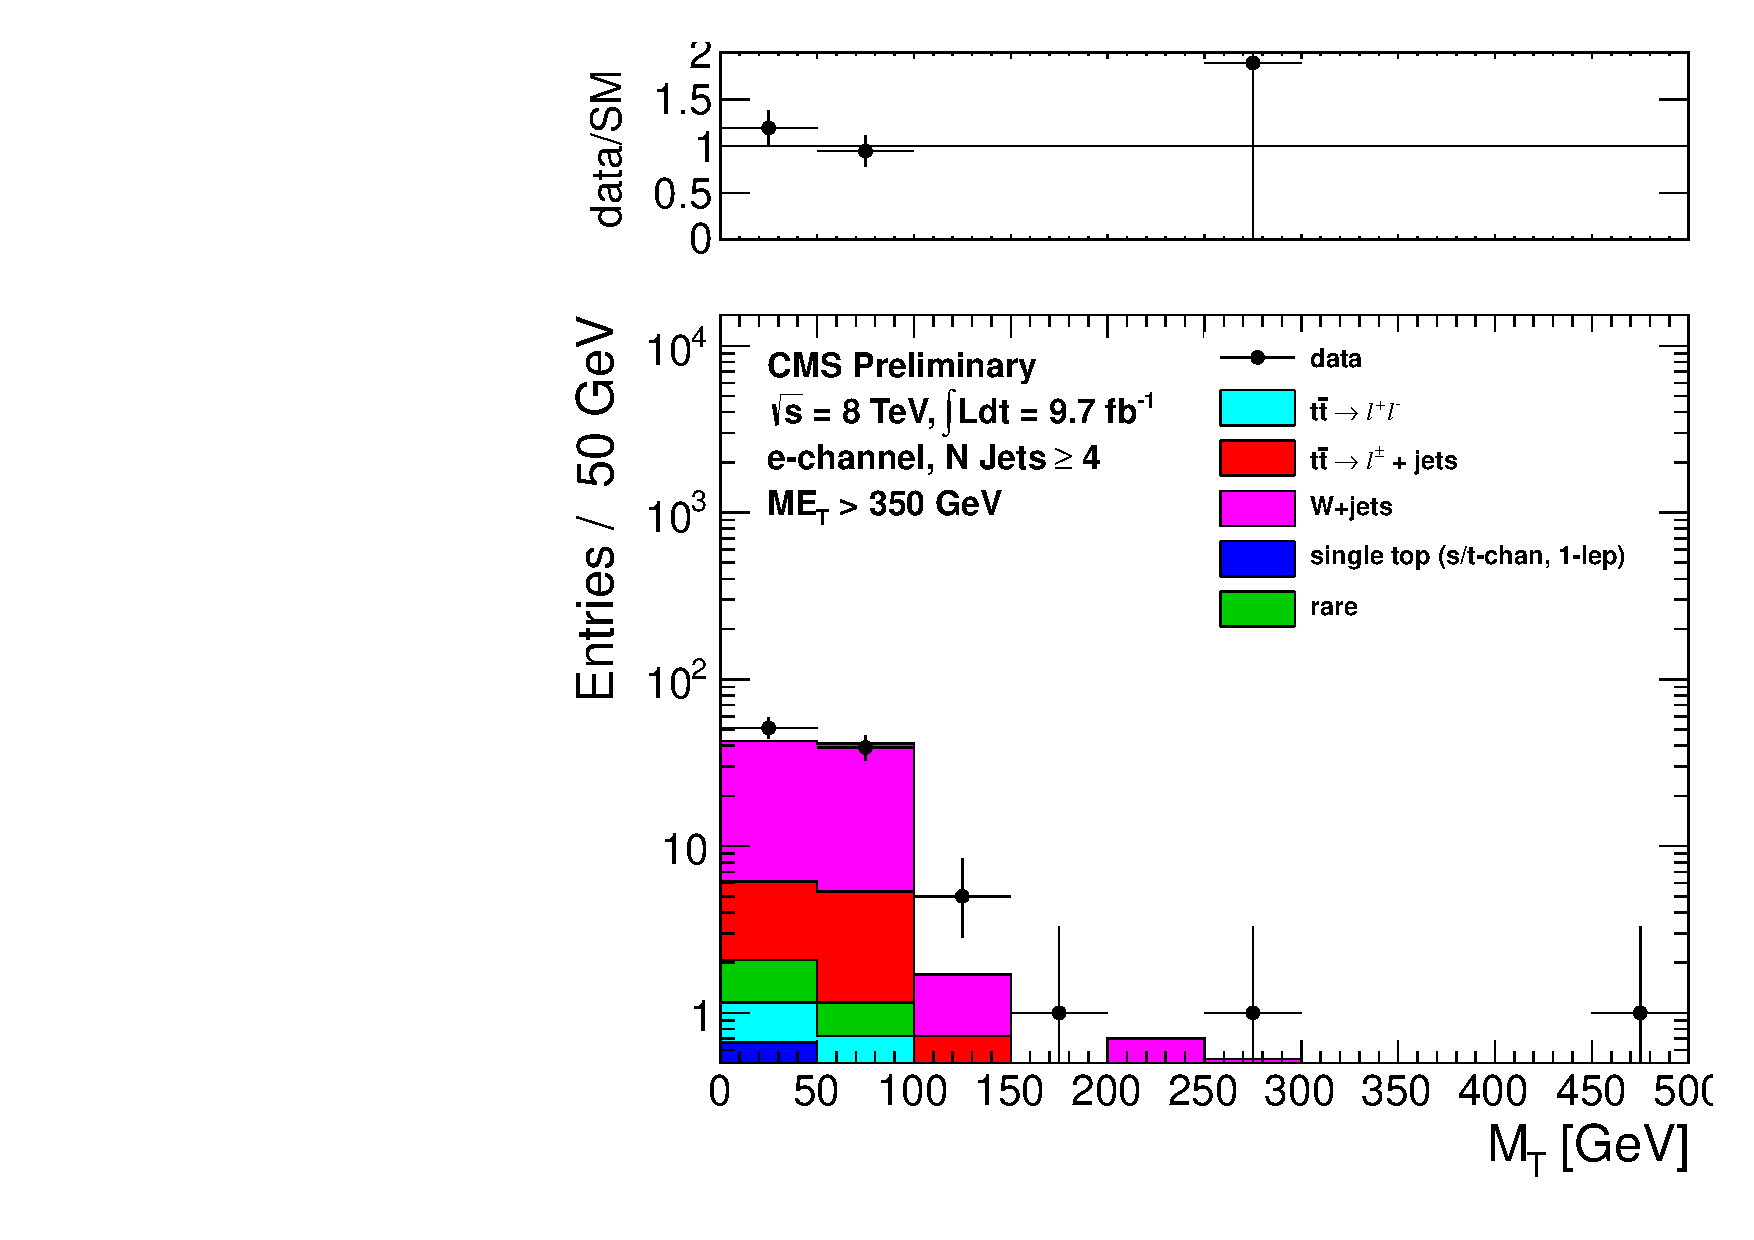
\includegraphics[width=0.5\linewidth]{plots/CR1plots/mt_met350_leadele_nj4.pdf}
        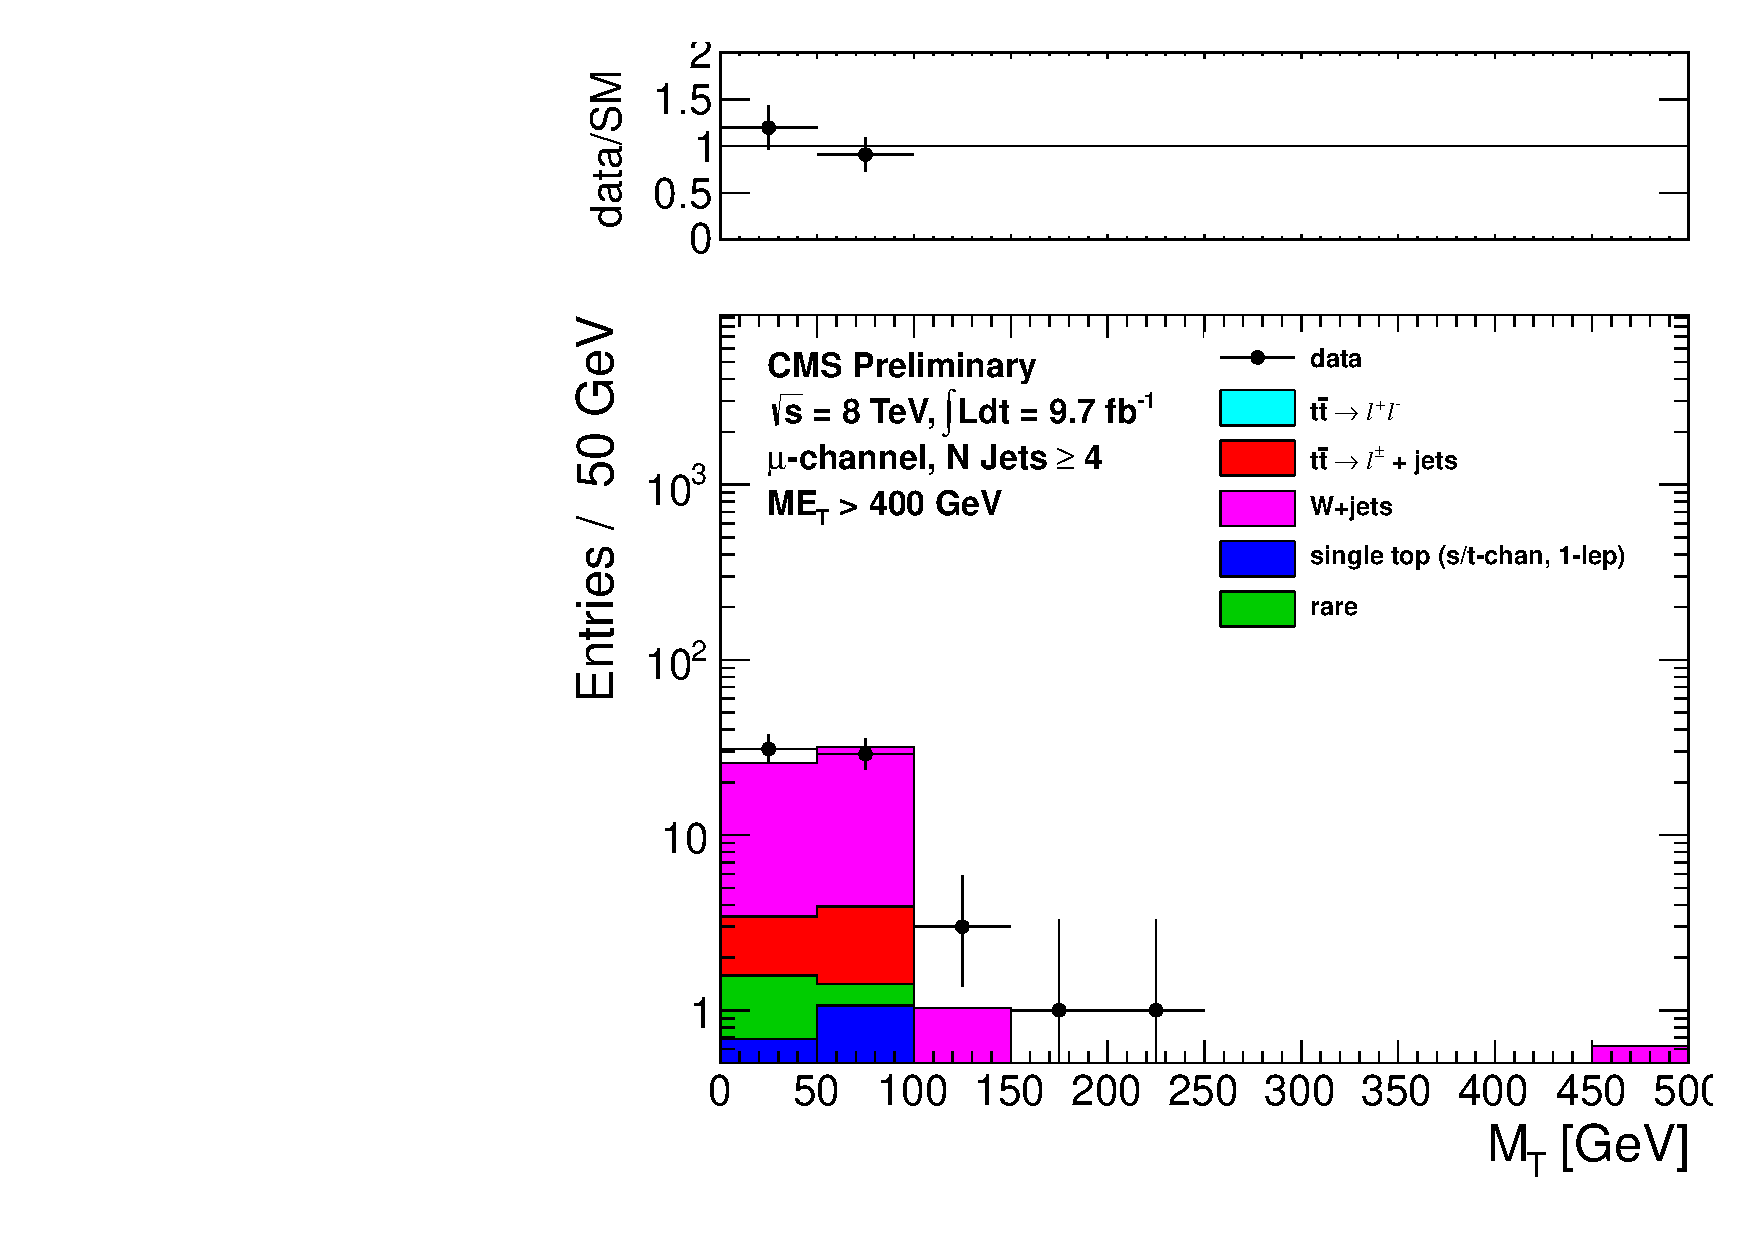
\includegraphics[width=0.5\linewidth]{plots/CR1plots/mt_met400_leadmuo_nj4.pdf}%
        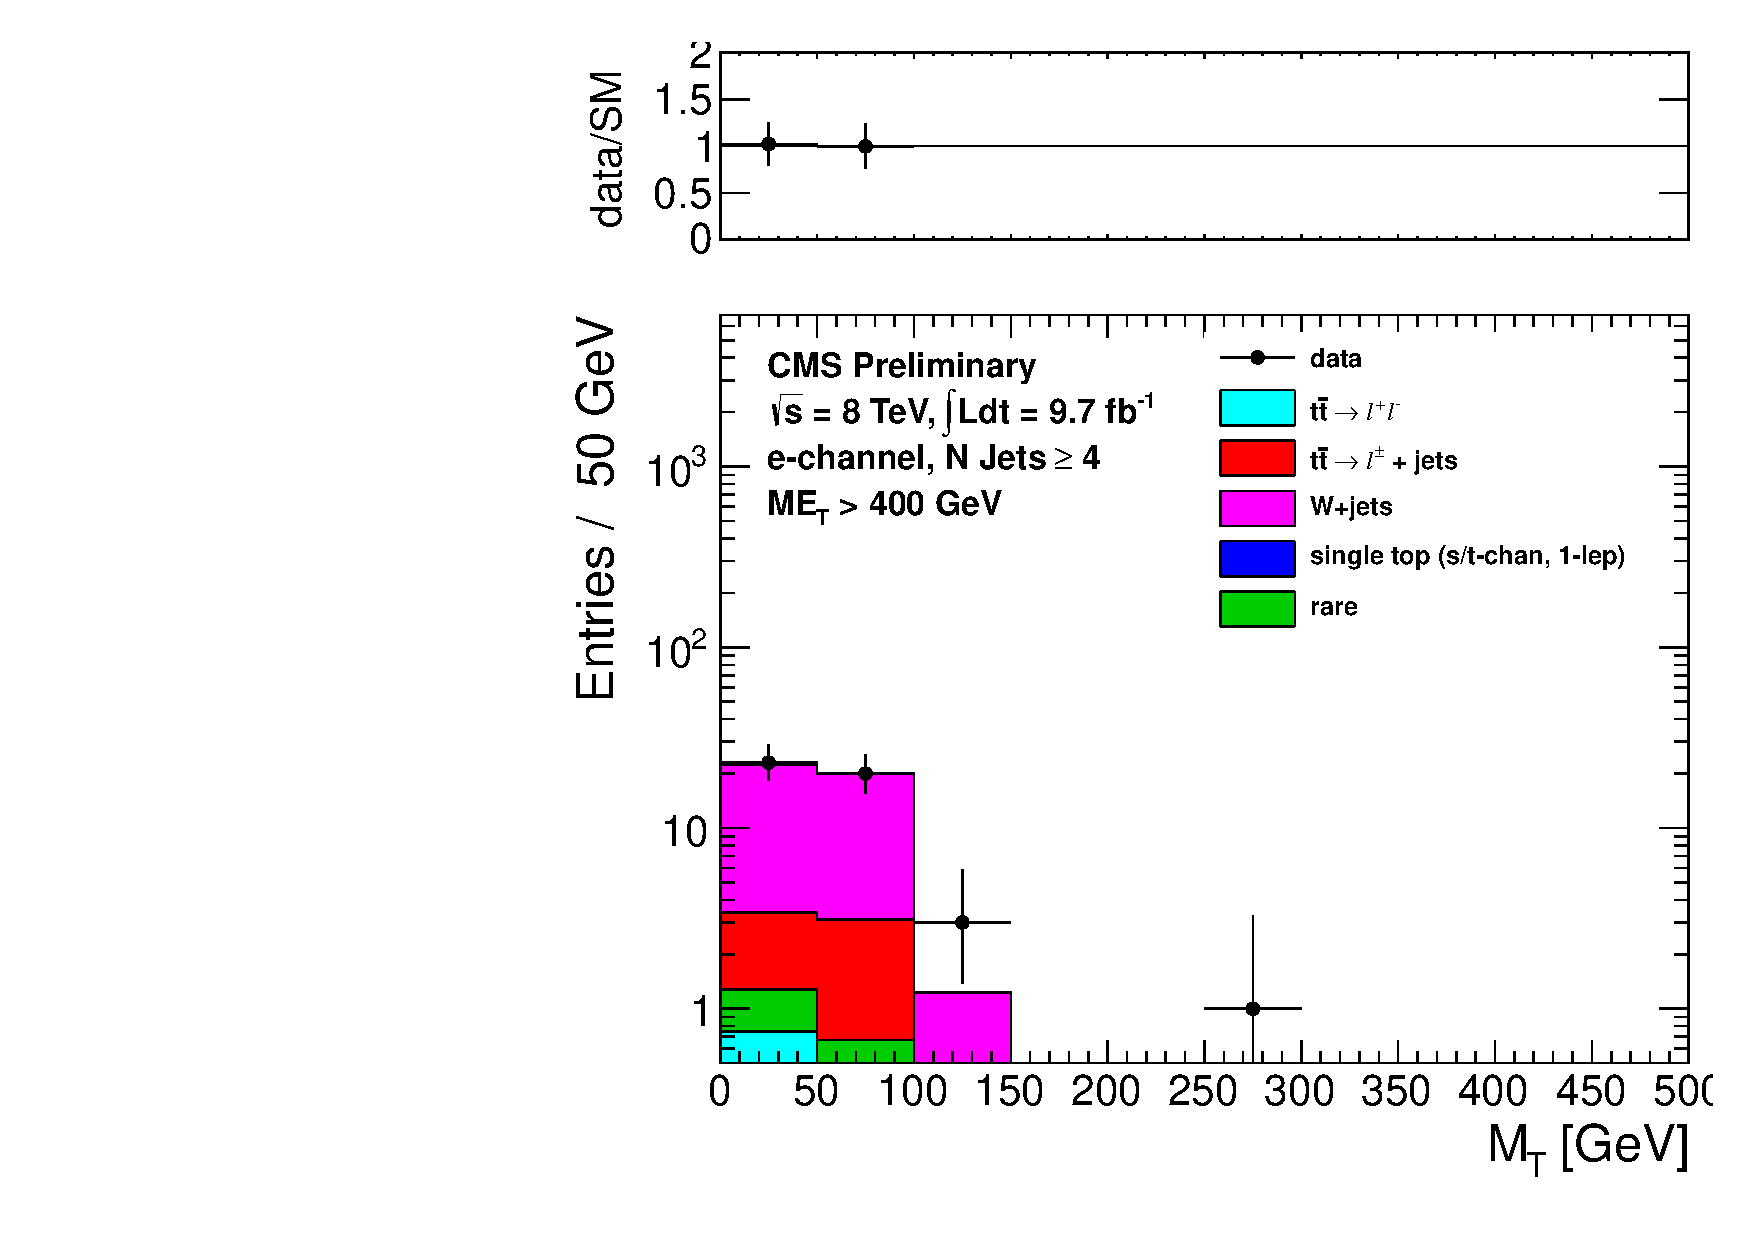
\includegraphics[width=0.5\linewidth]{plots/CR1plots/mt_met400_leadele_nj4.pdf}
    \caption{
      Comparison of the \mt\ distribution in data vs. MC for events
      with a leading muon (left) and leading electron (right)
      satisfying the requirements of CR1. The \met\ requirements used are
      300 GeV (top), 350 GeV (middle) and 400 GeV (bottom).
\label{fig:cr1mtrest2} 
}  
      \end{center}
\end{figure}


\clearpage

\subsection{Single Lepton Top MC Modelling Validation from CR2}
\label{sec:cr2}

IS THIS GOING TO BE DONE WITH A BVETO OR NOT.  IF SO, IS IT GOING TO
BE CSVL OR CSVM?  NEED TO DISCUSS THIS.

The \mt\ tail for single-lepton top events (\ttsl\ and single top) is dominated by jet resolution effects. The \W\ cannot be far off-shell because $\mW < \mtop$.
The modeling of the \mt\ tail from jet resolution effects is studied using \zjets\ data and MC samples. 
\Z\ events are selection by requiring 2 good leptons (satisfying ID and isolation requirements) and requiring the \mll\ to be in the range $81-101$ GeV. 
The negative lepton is treated as a neutrino and so is added to the MET: \met\ $\rightarrow$ \pt(\Lepm) + \met, 
and the \mt\ is recalculated with the positive lepton \mt(\Lepp, \met).
The resulting ``pseudo-\mt'' is dominated by jet resolution effects, since no off-shell 
\Z\ production enters the sample due to the \mll\ requirement.
This section describes how well the MC predicts the tail of ``pseudo-\mt''. 

The underlying distributions are shown in Fig.~\ref{fig:cr2met}
and~\ref{fig:cr2mtrest}.  The comparison of data and MC event counts 
is shown in Table~\ref{tab:cr2yields}.  From this table we extract
the data to MC scale factors $SFR^{e}_{top}$ and  $SFR^{\mu}_{top}$. 


\begin{table}[!h]
\begin{center}
{\footnotesize
\begin{tabular}{l||c|c||c|c|c|c|c}
\hline
Sample              & CR2PRESEL0 &CR2PRESEL1 & CR2A & CR2B & CR2C &
CR2D & CR2E\\
\hline
\hline
DY MC 		  & $26 \pm 2$ & $22 \pm 2$ & $15 \pm 2$ & $28 \pm 3$ & $10 \pm 2$ & $3 \pm 1$ & $1 \pm 1$ \\
Data - non-DY MC 	  & $47 \pm 8$ & $36 \pm 7$ & $28 \pm 6$ & $35 \pm 6$ & $19 \pm 5$ & $11 \pm 3$ & $1 \pm 1$ \\
\hline
Data/MC SF 	  & $1.77 \pm 0.31$ & $1.61 \pm 0.33$ & $1.91 \pm 0.45$ & $1.25 \pm 0.27$ & $1.93 \pm 0.60$ & $3.38 \pm 1.70$ & $1.30 \pm 1.56$ \\
\hline
\end{tabular}}
\caption{ Yields in \mt\ tail comparing the MC prediction (after
  applying SFs) to data. CR2PRESEL refers to a sample with $\met>50$
  GeV and $\mt>150$ GeV.
  The uncertainties are statistical only.  NEED TO ADD THE SYMBOLS
  DEFINED IN THE TEXT FOR THESE SCALE FACTORS.  IS THIS GOING TO BE
  DONE SEPARATELY FOR MUONS AND ELECTRONS???
  MAYBE WANT TO REMOVE LAST ENTRIES WHERE STATS ARE VERY LOW
\label{tab:cr2yields}}
\end{center}
\end{table}

\begin{figure}[hbt]
  \begin{center}
%	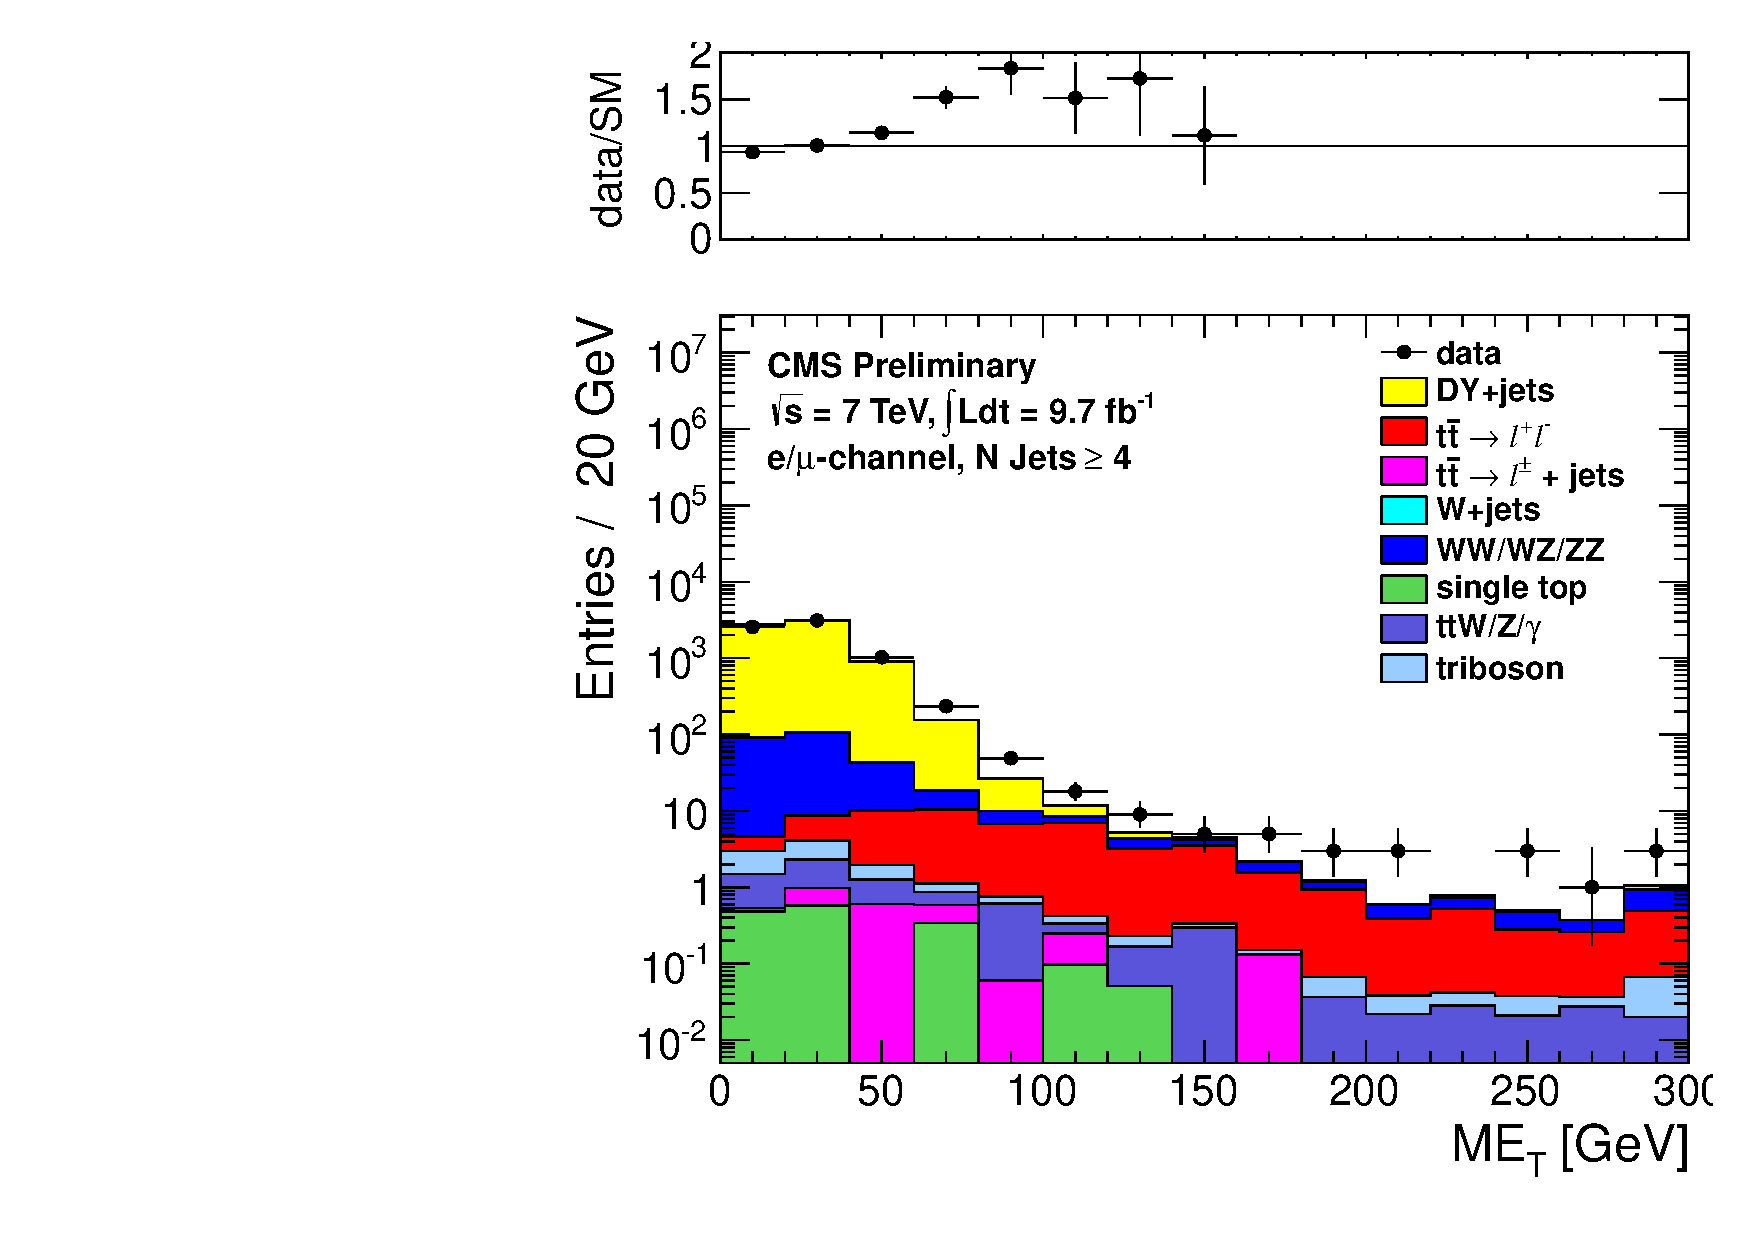
\includegraphics[width=0.5\linewidth]{plots/CR2plots/met_scaled_nj4_emucomb.pdf}%
	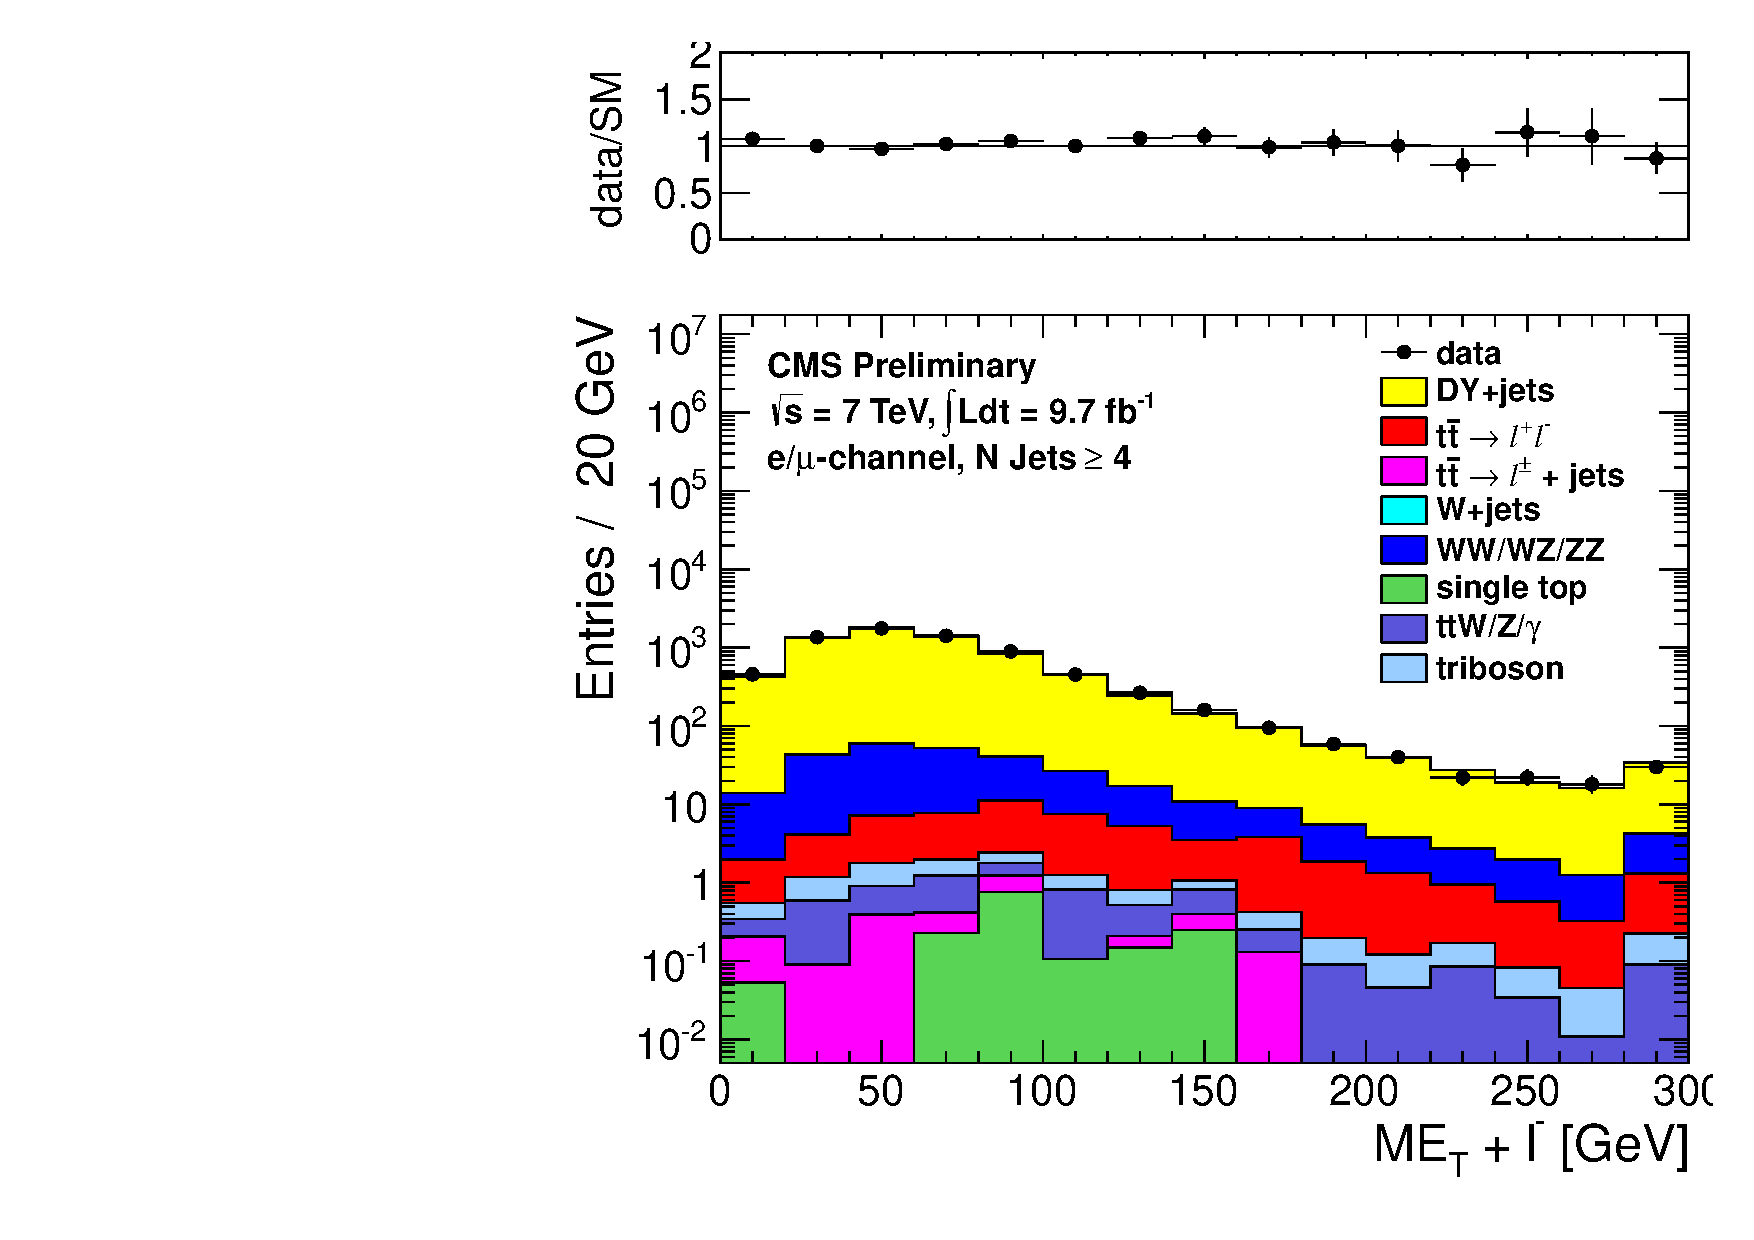
\includegraphics[width=0.5\linewidth]{plots/CR2plots/met_lepcor_scaled_nj4_emucomb.pdf}%
	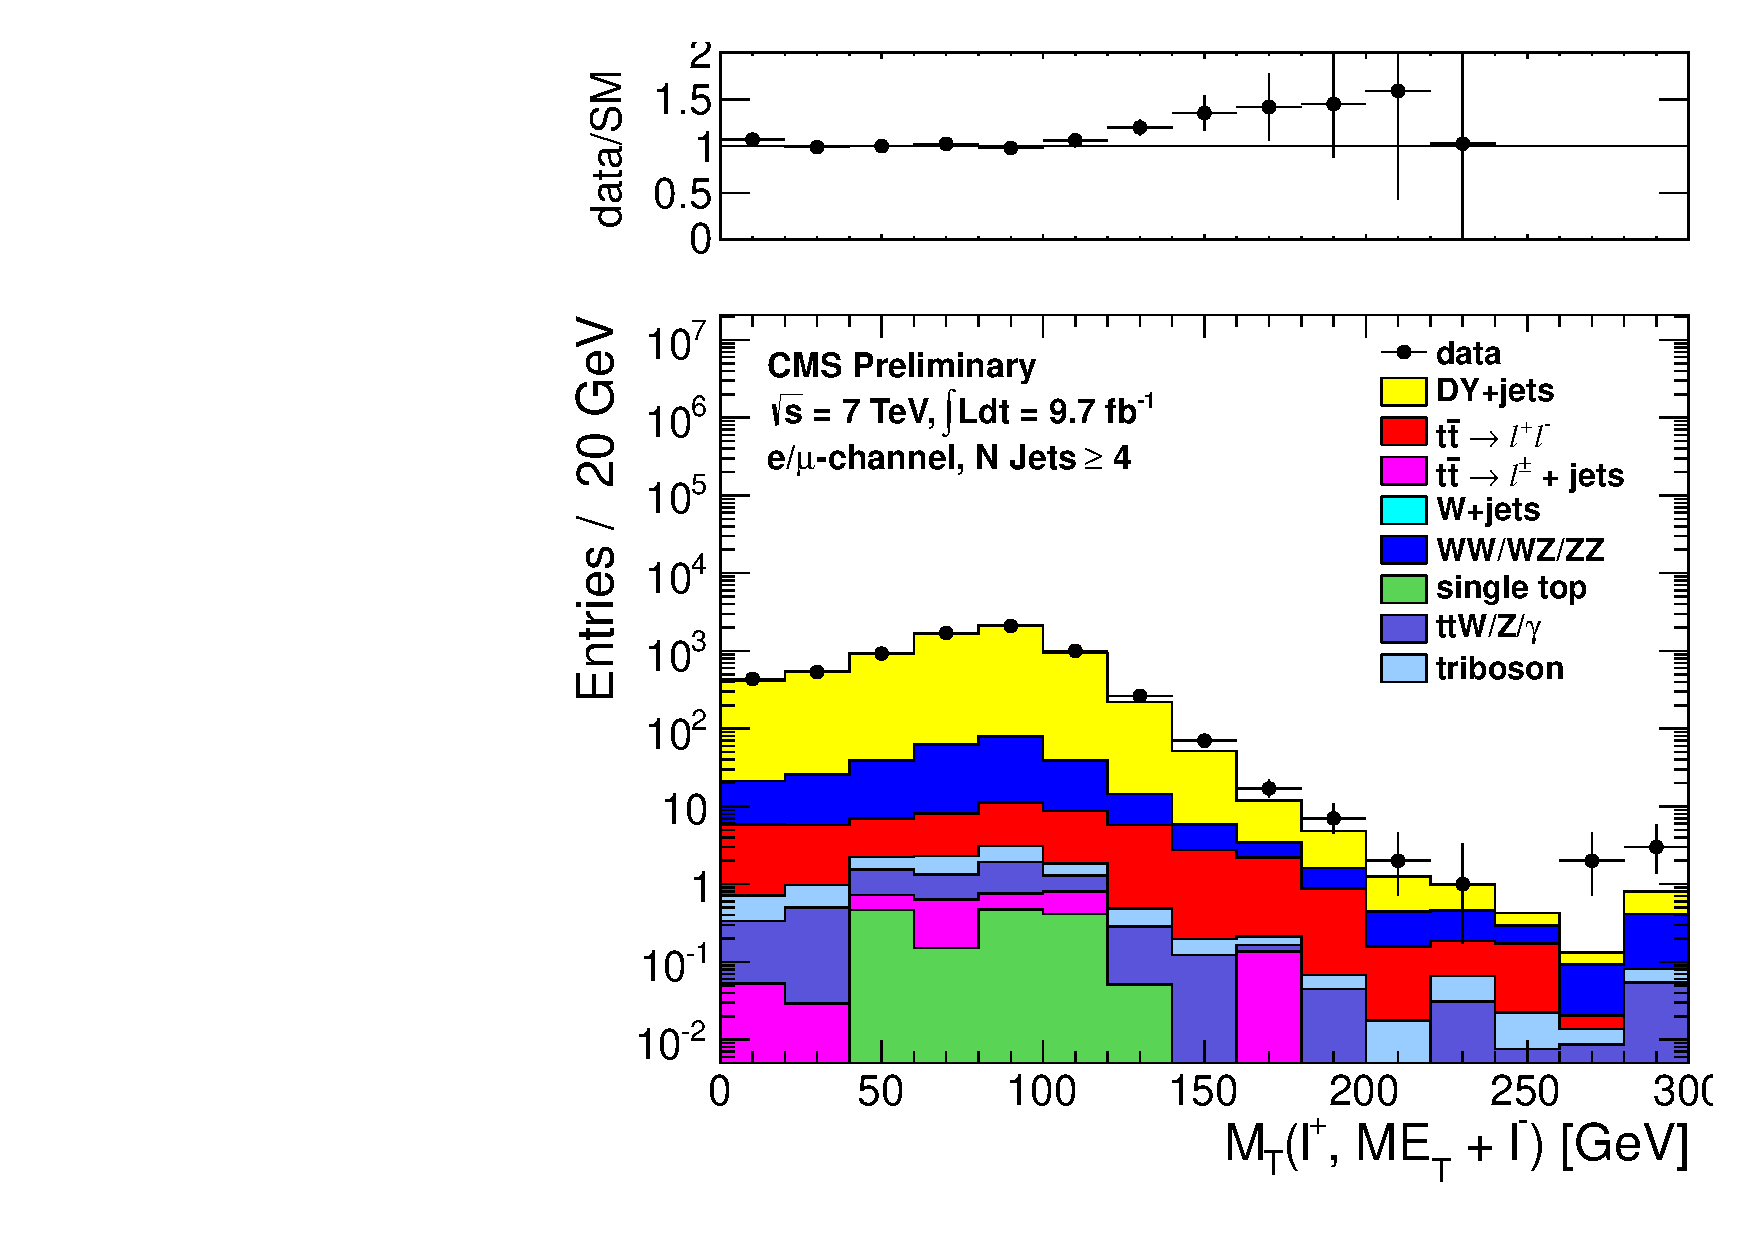
\includegraphics[width=0.5\linewidth]{plots/CR2plots/mt_lepcor_scaled_nj4_emucomb.pdf}
	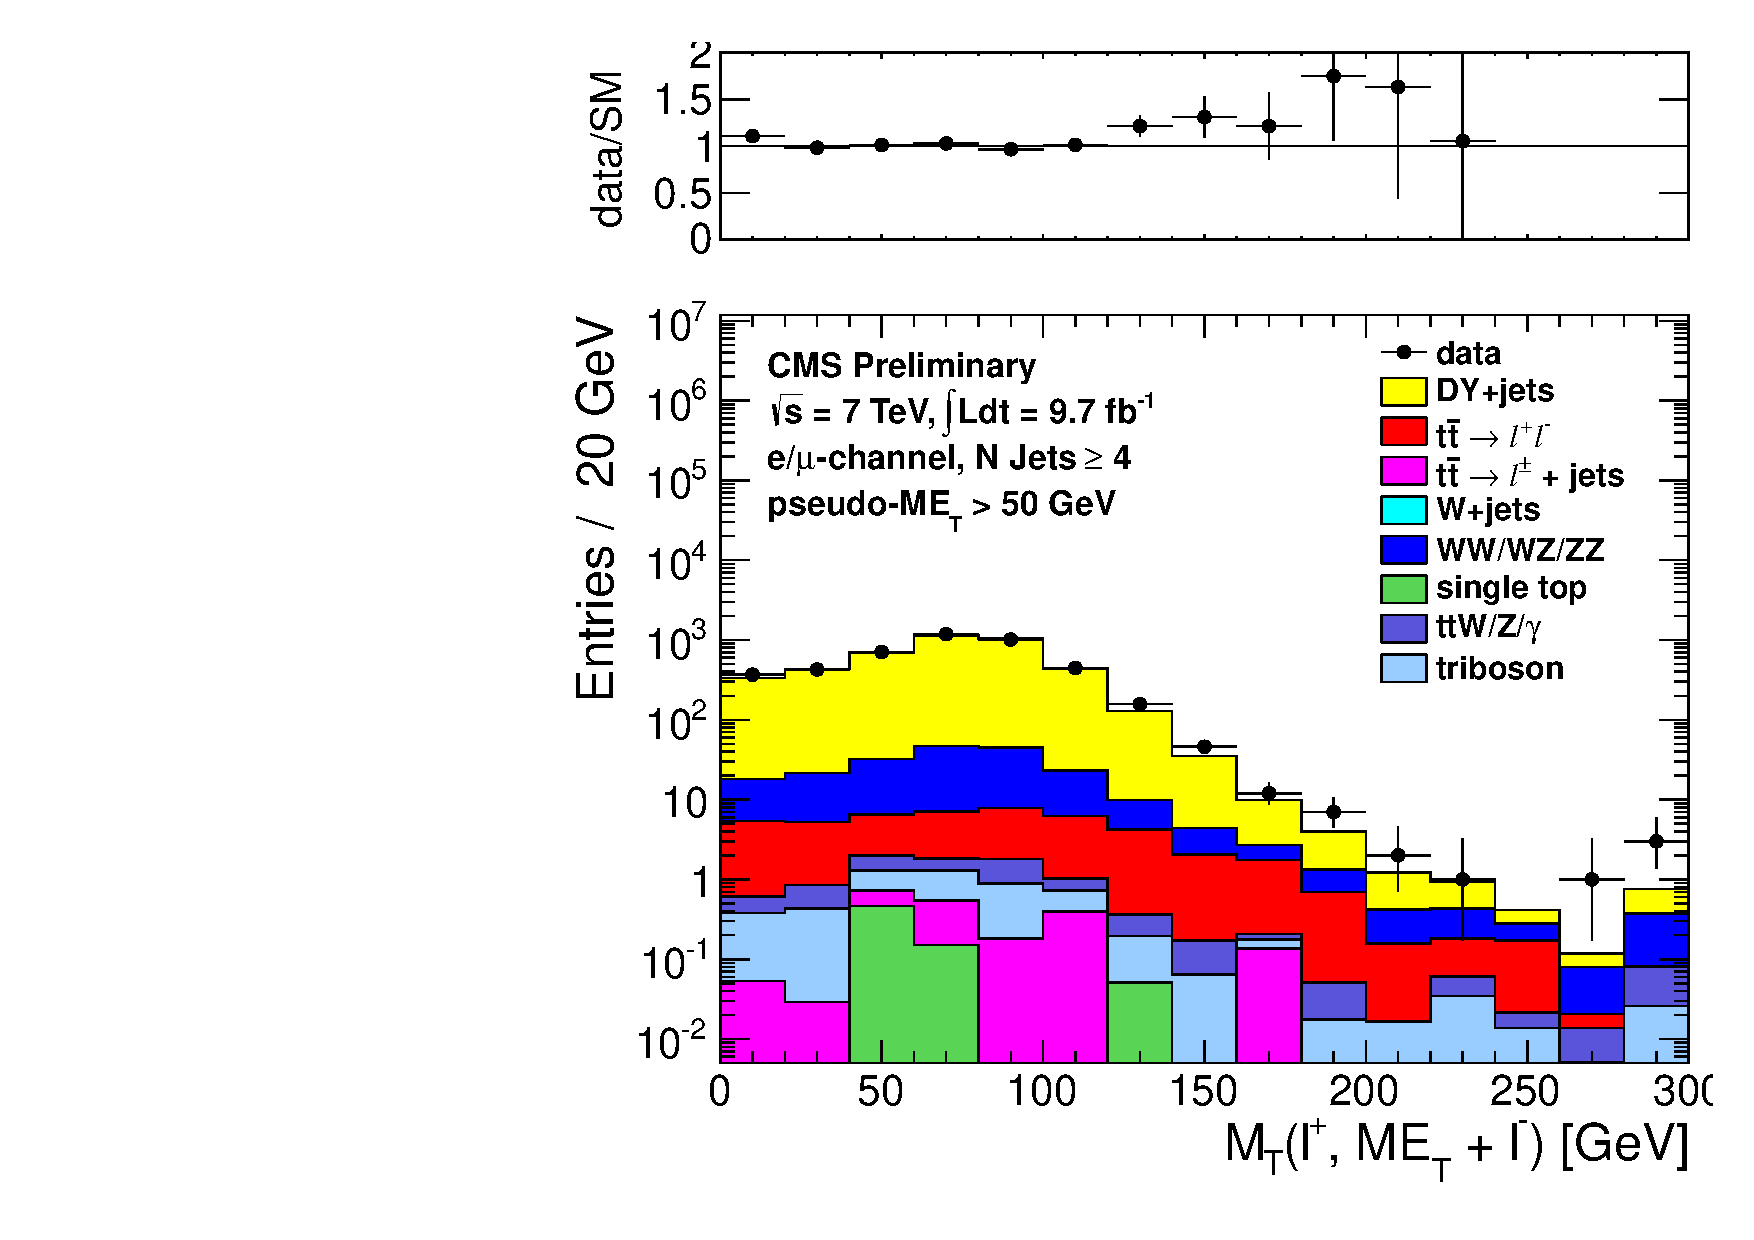
\includegraphics[width=0.5\linewidth]{plots/CR2plots/mt_lepcor_scaled_met50_nj4_emucomb.pdf}%
	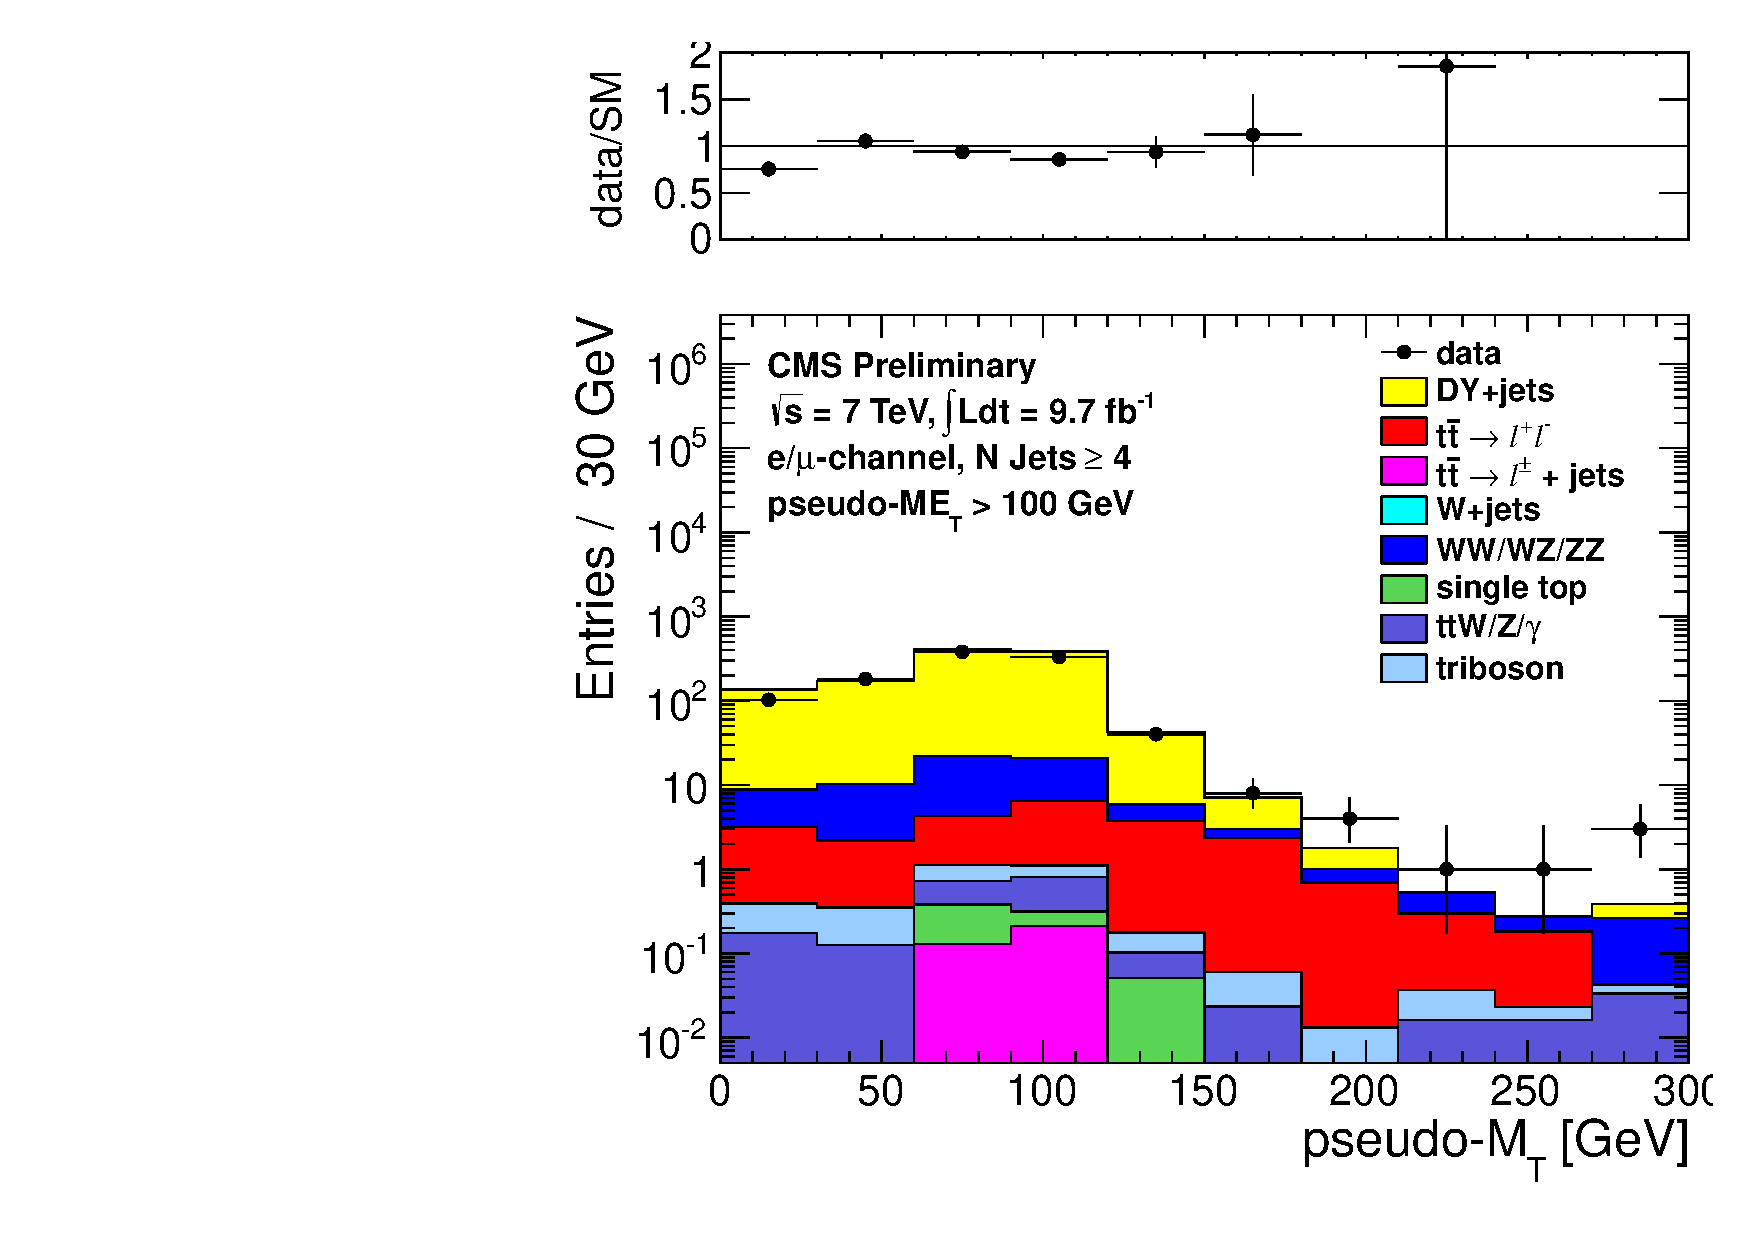
\includegraphics[width=0.5\linewidth]{plots/CR2plots/mt_lepcor_scaled_met100_nj4_emucomb.pdf}

    \caption{
      Comparison of the pseudo\-\met\ (top, left), pseudo\-\mt\ (top,
      right and bottom) distributions in data vs. MC for events
      satisfying the requirements of CR2, combining both the muon and
      electron channels. The pseudo\-\mt\ distributions are shown
      before any additional requirements (top, right) and after
      requiring pseudo\-\met>50 GeV (bottom, left) and pseudo\-\met>100 GeV (bottom, right) .
\label{fig:cr2met} 
}  
      \end{center}
\end{figure}

\begin{figure}[hbt]
  \begin{center}
	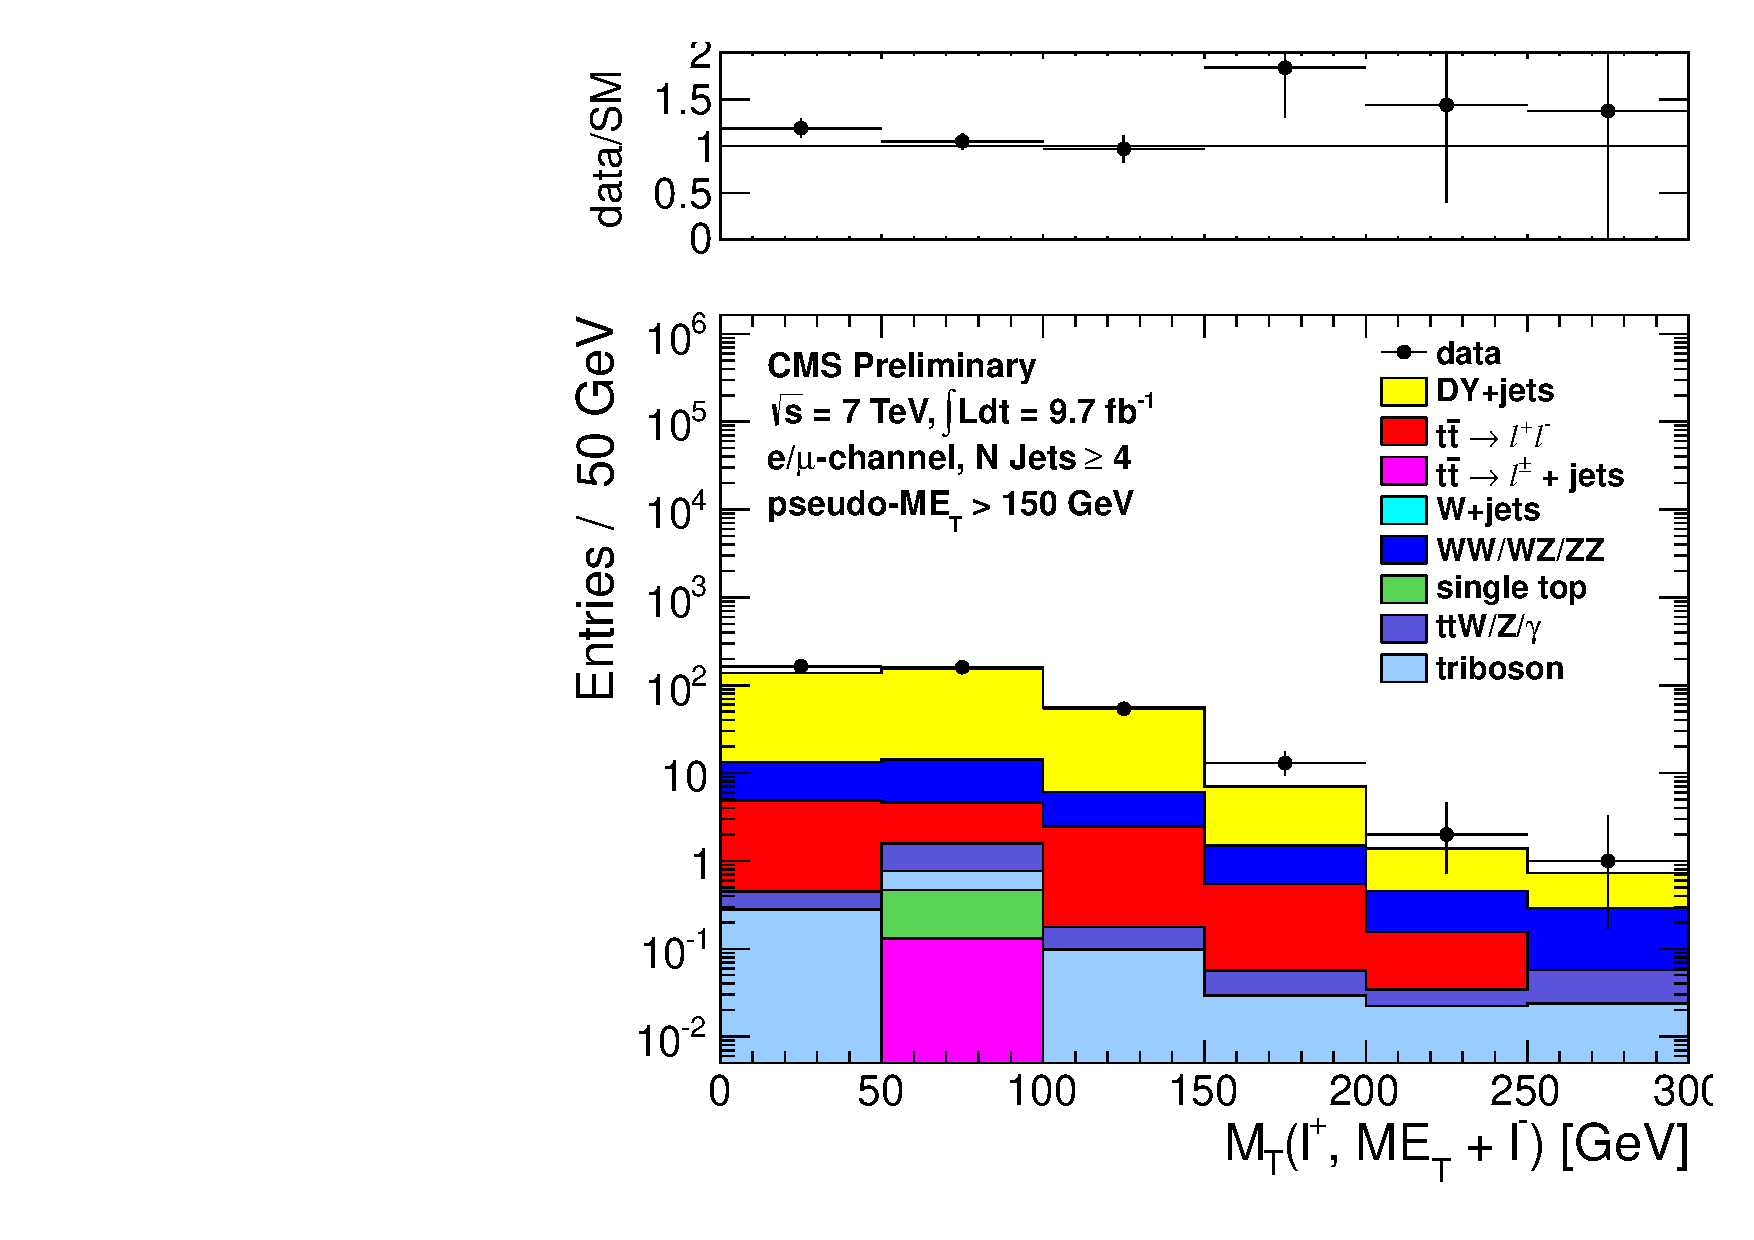
\includegraphics[width=0.5\linewidth]{plots/CR2plots/mt_lepcor_scaled_met150_nj4_emucomb.pdf}%
	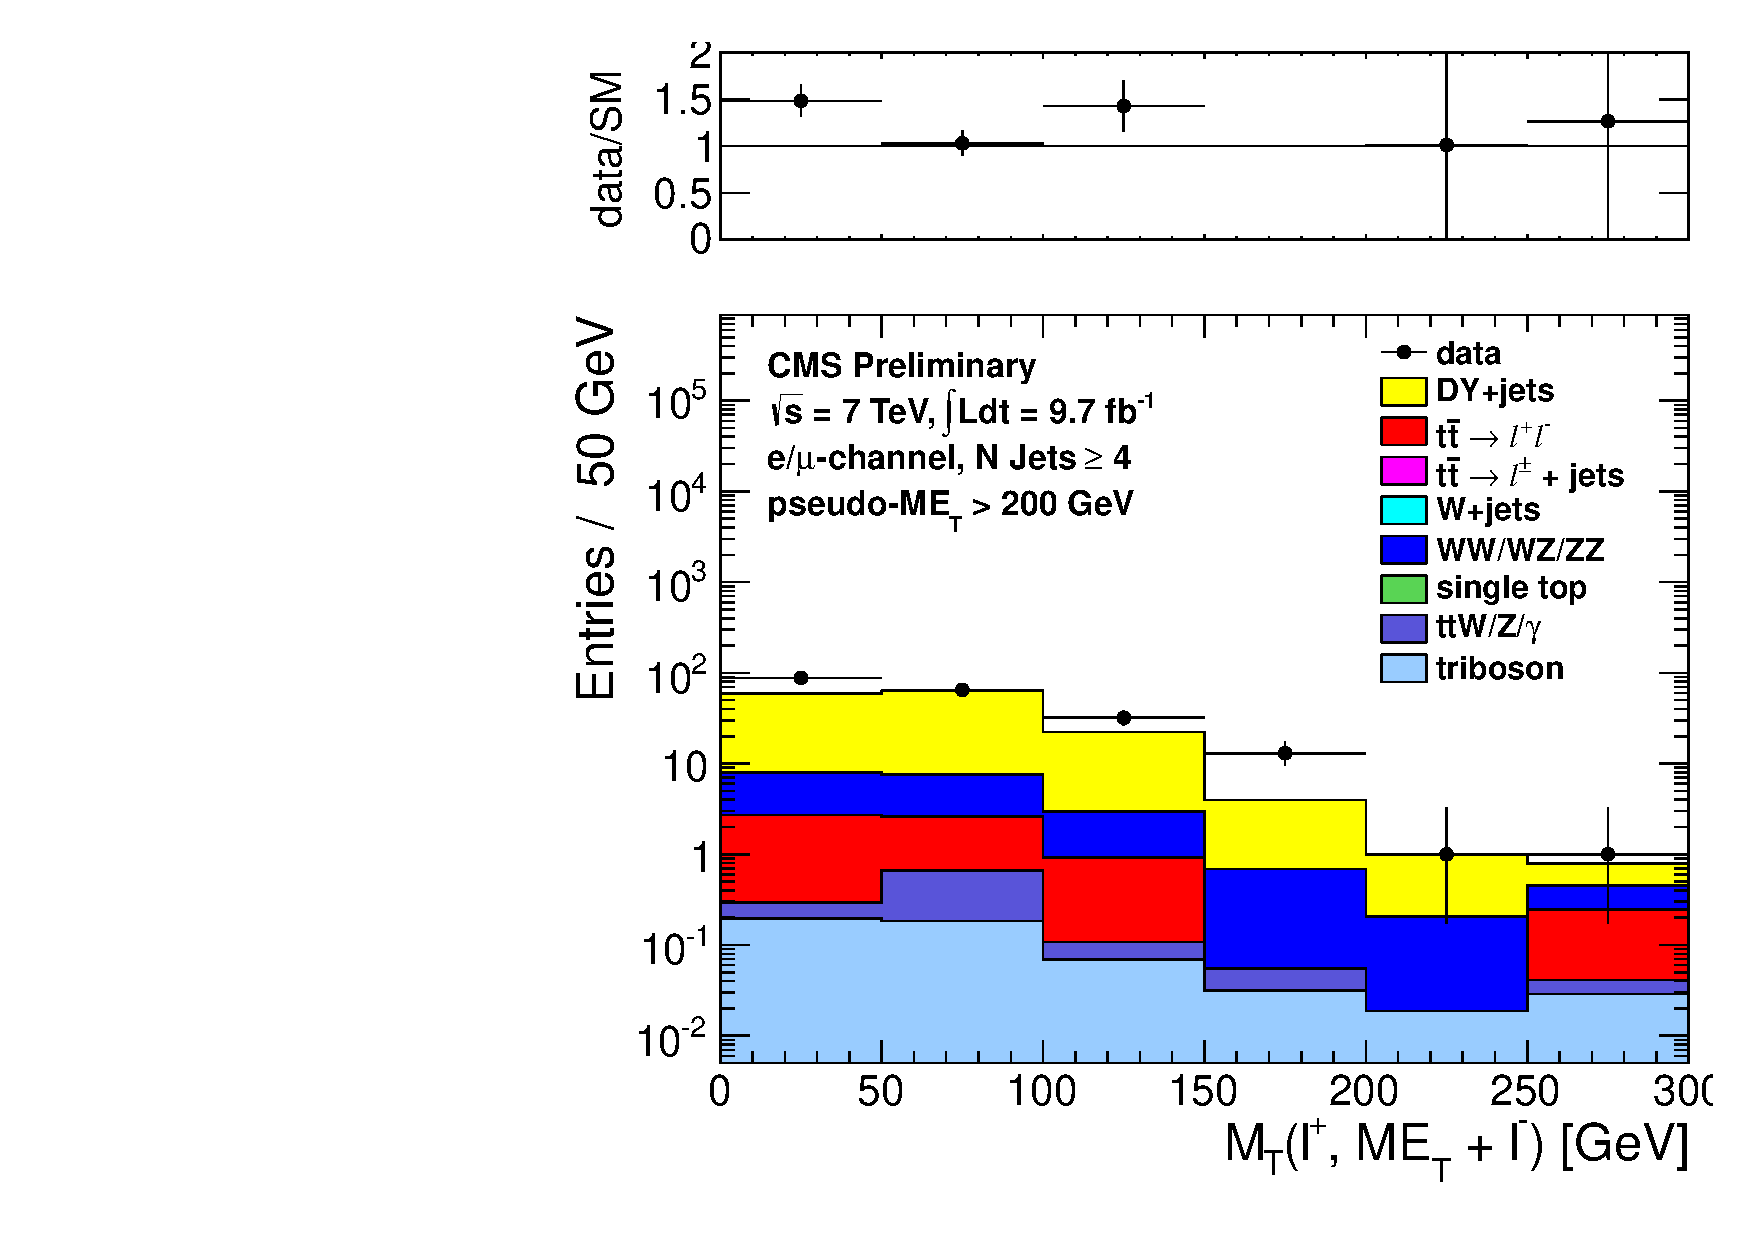
\includegraphics[width=0.5\linewidth]{plots/CR2plots/mt_lepcor_scaled_met200_nj4_emucomb.pdf}
	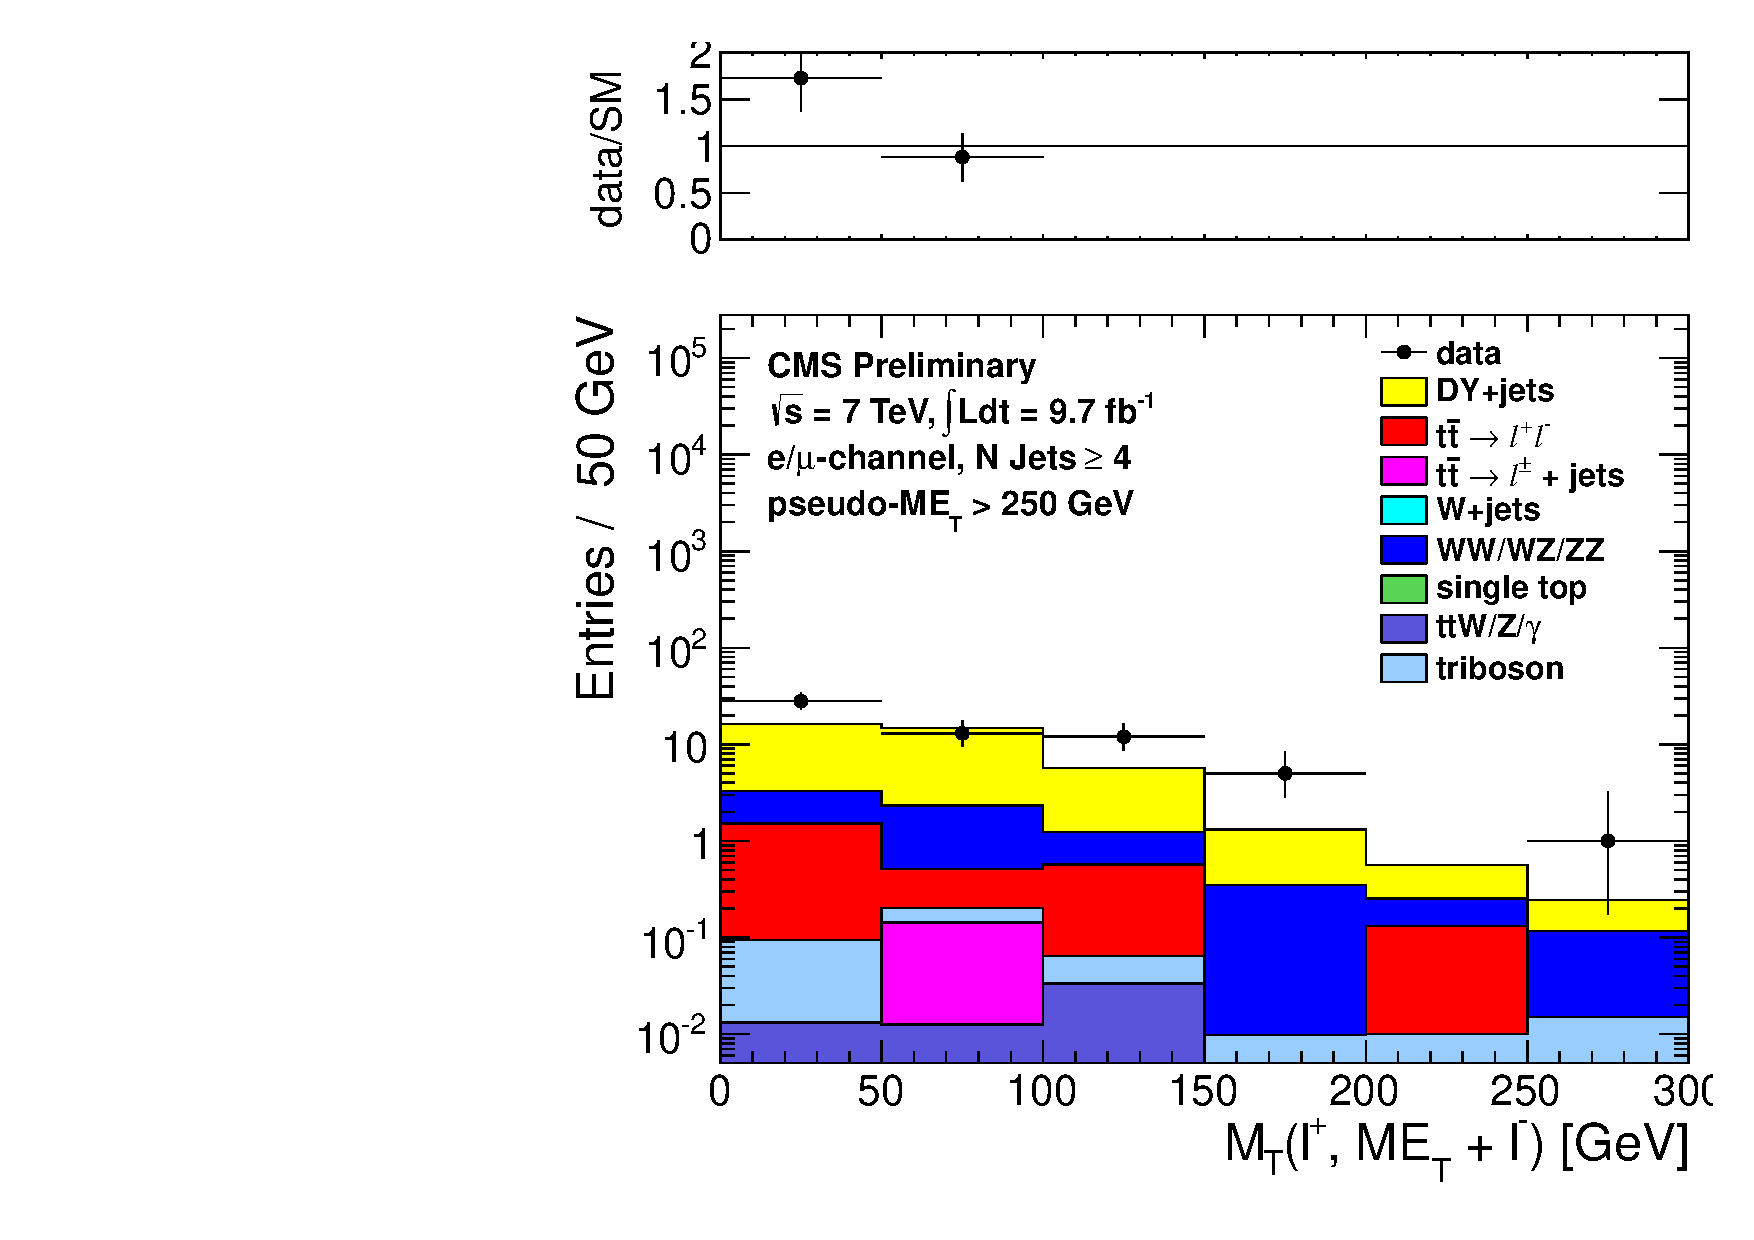
\includegraphics[width=0.5\linewidth]{plots/CR2plots/mt_lepcor_scaled_met250_nj4_emucomb.pdf}%
	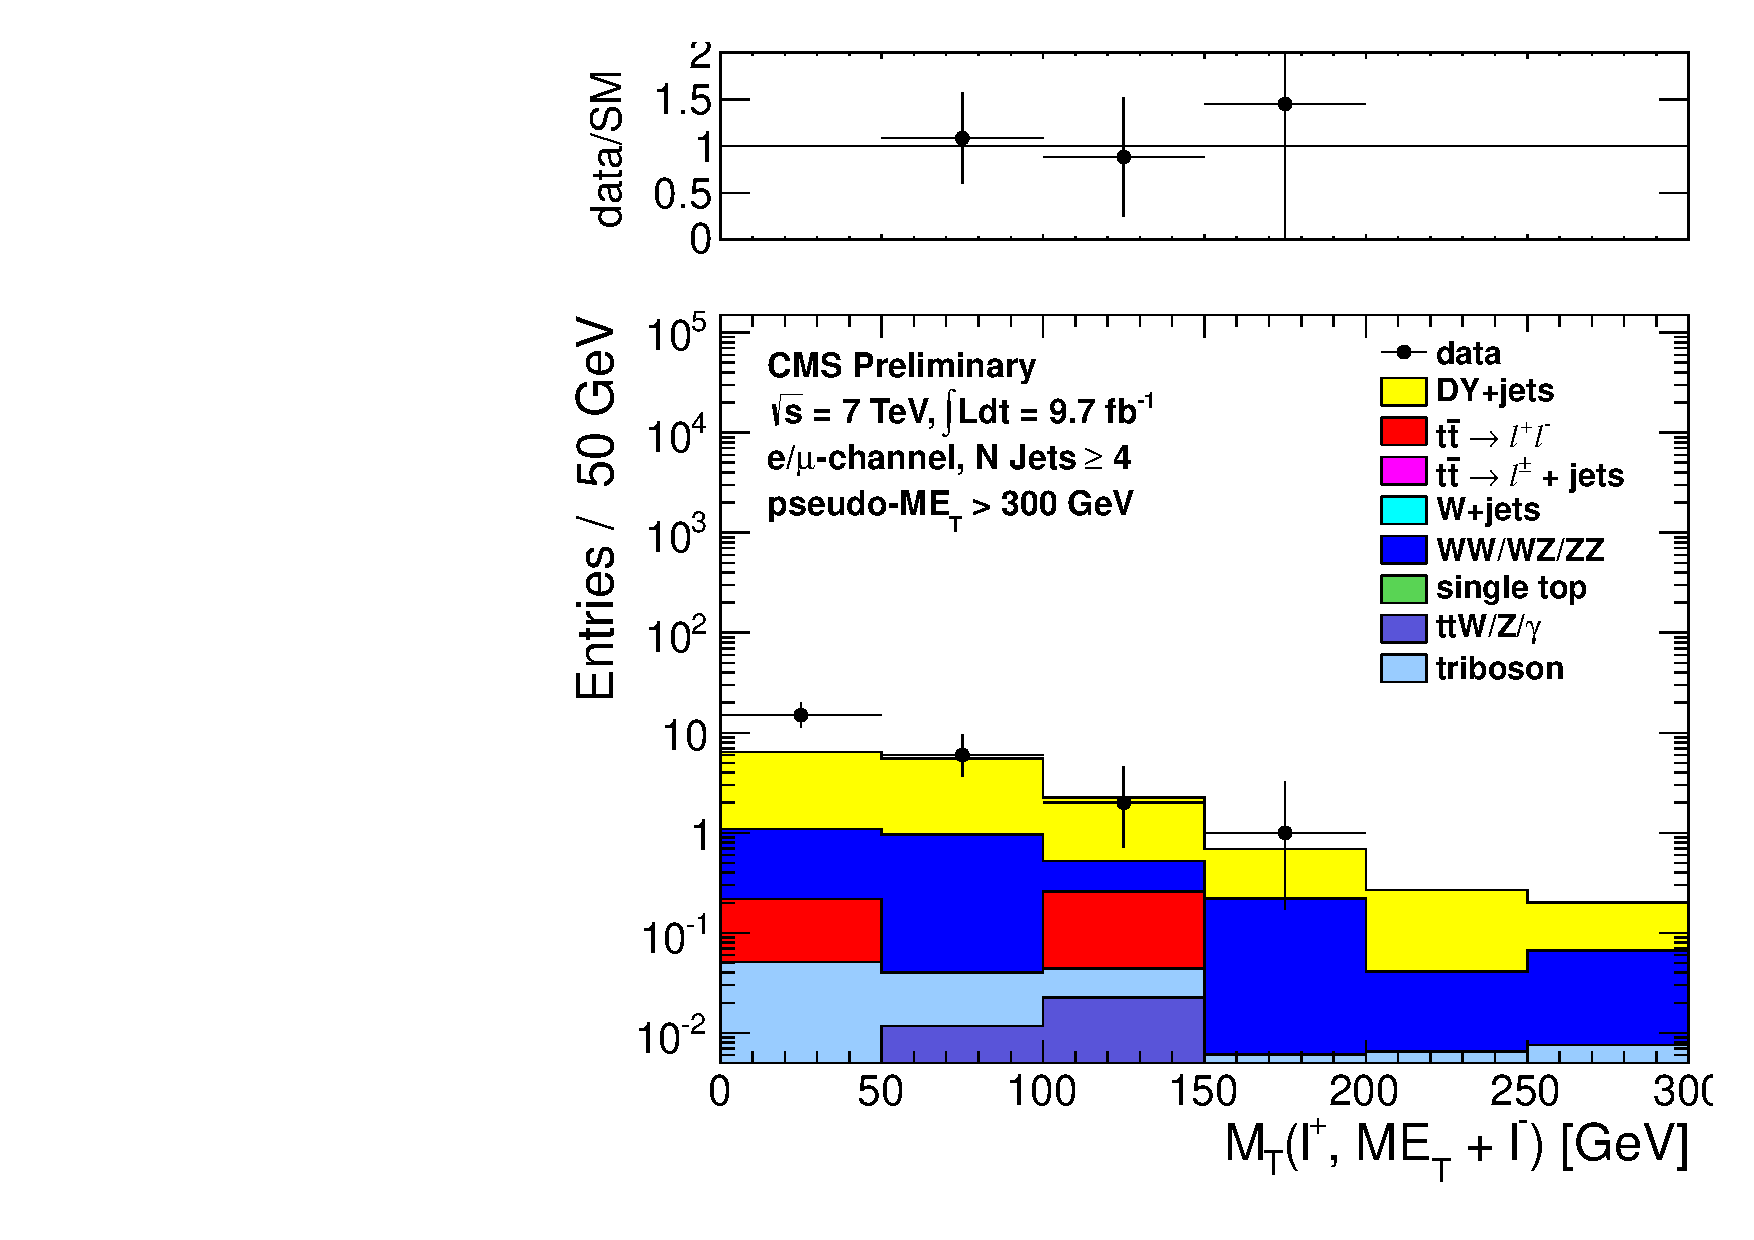
\includegraphics[width=0.5\linewidth]{plots/CR2plots/mt_lepcor_scaled_met300_nj4_emucomb.pdf}
    \caption{
      Comparison of the \mt\ distribution in data vs. MC for events
      satisfying the requirements of CR2, combining both the muon and
      electron channels. The pseudo-\met\ requirements used are
      150 GeV (top, left), 200 GeV (top, right), 250 GeV (bottom,
      left) and 300 GeV (bottom, right).
\label{fig:cr2mtrest} 
}  
      \end{center}
\end{figure}
\clearpage
\subsection{Dilepton studies in CR4}
\label{sec:cr4}

\subsubsection{Modeling of Additional Hard Jets in Top Dilepton Events}
\label{sec:jetmultiplicity}

[THIS SUBSUBSECTION IS DONE...MODULO THE LATEST PLOTS AND THE LATEST
NUMBERS IN THE TABLE]

Dilepton \ttbar\ events have 2 jets from the top decays, so additional
jets from radiation or higher order contributions are required to
enter the signal sample. The modeling of addtional jets in \ttbar\
events is checked in a \ttll\ control sample,
selected by requiring
\begin{itemize}
\item exactly 2 selected electrons or muons with \pt $>$ 20 GeV
\item \met\ $>$ 100 GeV
\item $\geq1$ b-tagged jet
\item Z-veto ($|m_{\ell\ell} - 91| > 15$ GeV)
\end{itemize}
Figure~\ref{fig:dileptonnjets} shows a comparison of the jet
multiplicity distribution in data and MC for this two-lepton control
sample. After requiring at least 1 b-tagged jet, most of the
events have 2 jets, as expected from the dominant process \ttll. There is also a
significant fraction of events with additional jets. 
The 3-jet sample is mainly comprised of \ttbar\ events with 1 additional
emission and similarly the $\ge4$-jet sample contains primarily
$\ttbar+\ge2$ jet events. 
%Even though the primary \ttbar\
%Madgraph sample used includes up to 3 additional partons at the Matrix
%Element level, which are intended to describe additional hard jets,
%Figure~\ref{fig:dileptonnjets} shows a slight mis-modeling of the
%additional jets. 


\begin{figure}[hbt]
  \begin{center}
	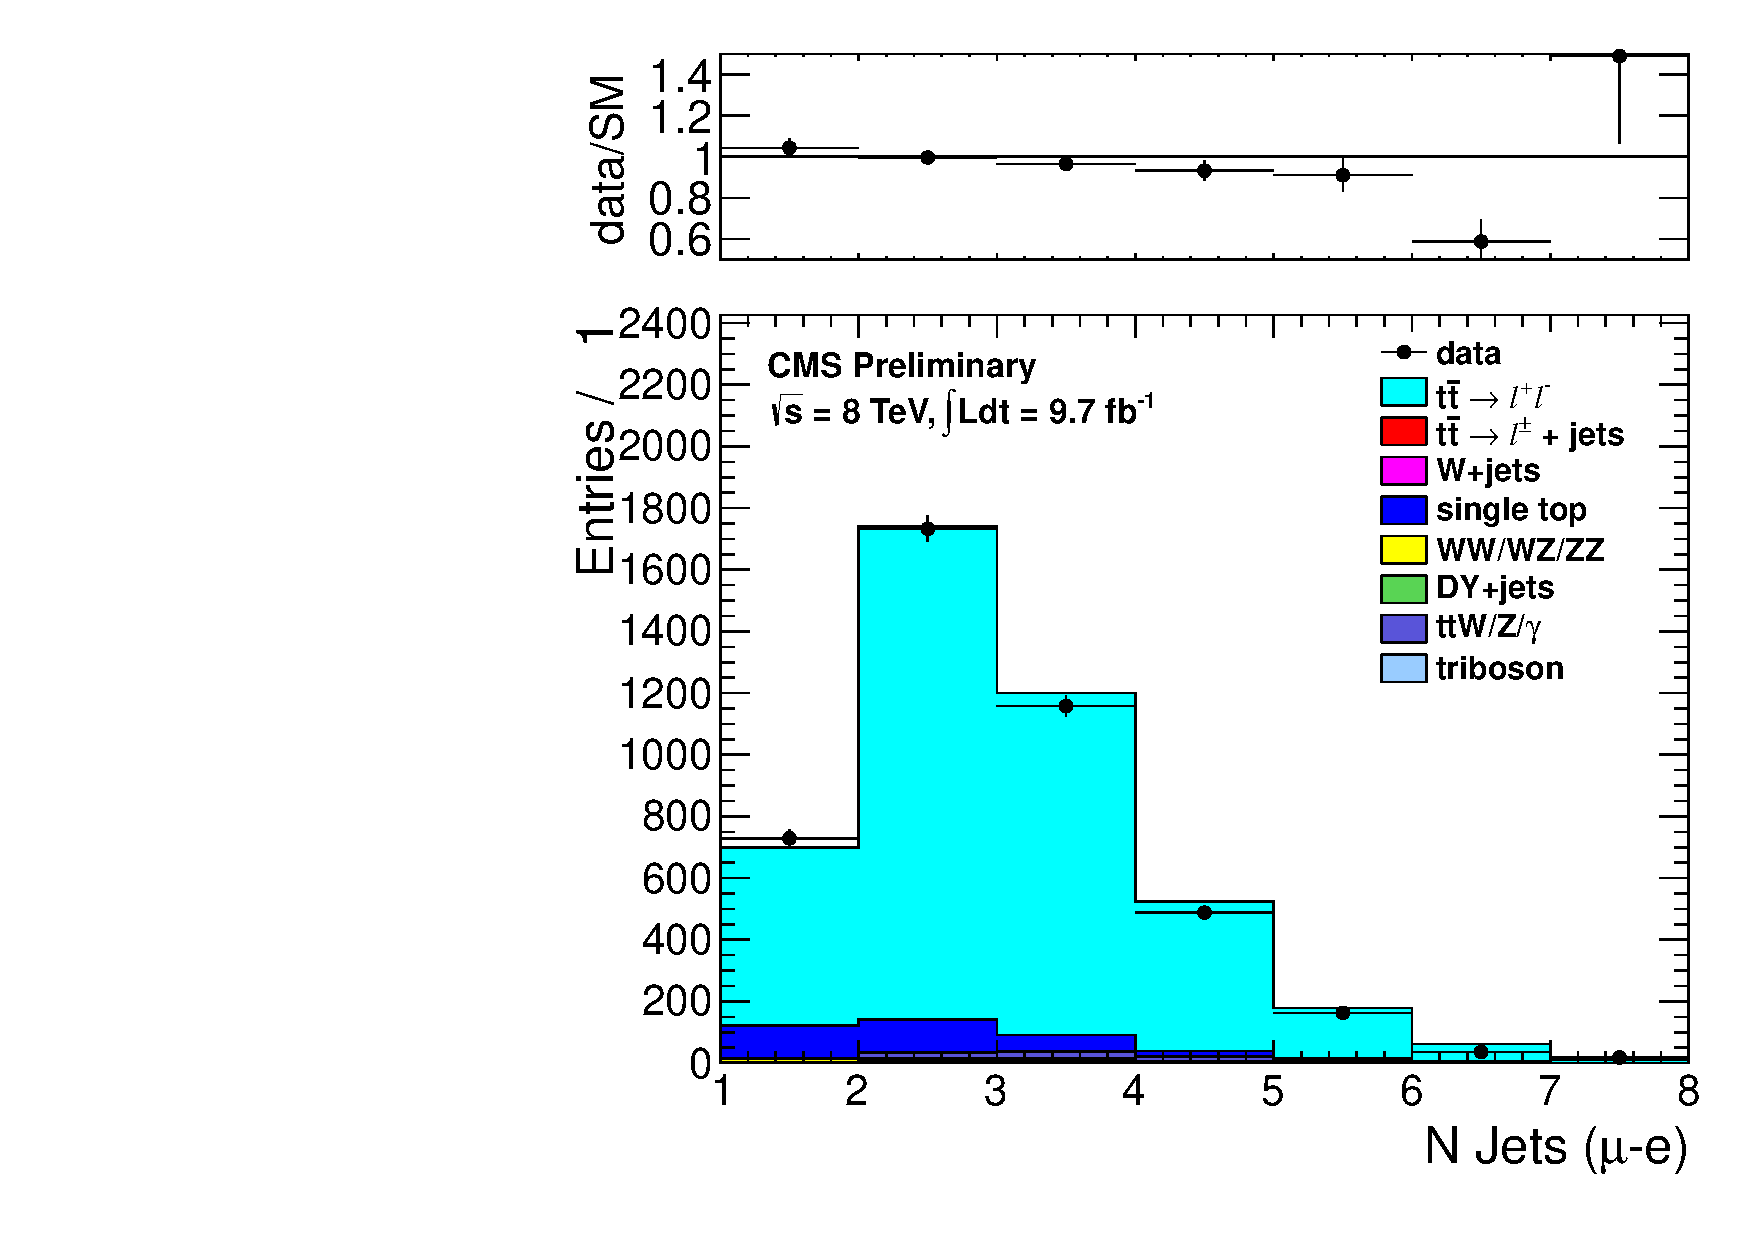
\includegraphics[width=0.5\linewidth]{plots/njets_all_met100_mueg.pdf}
	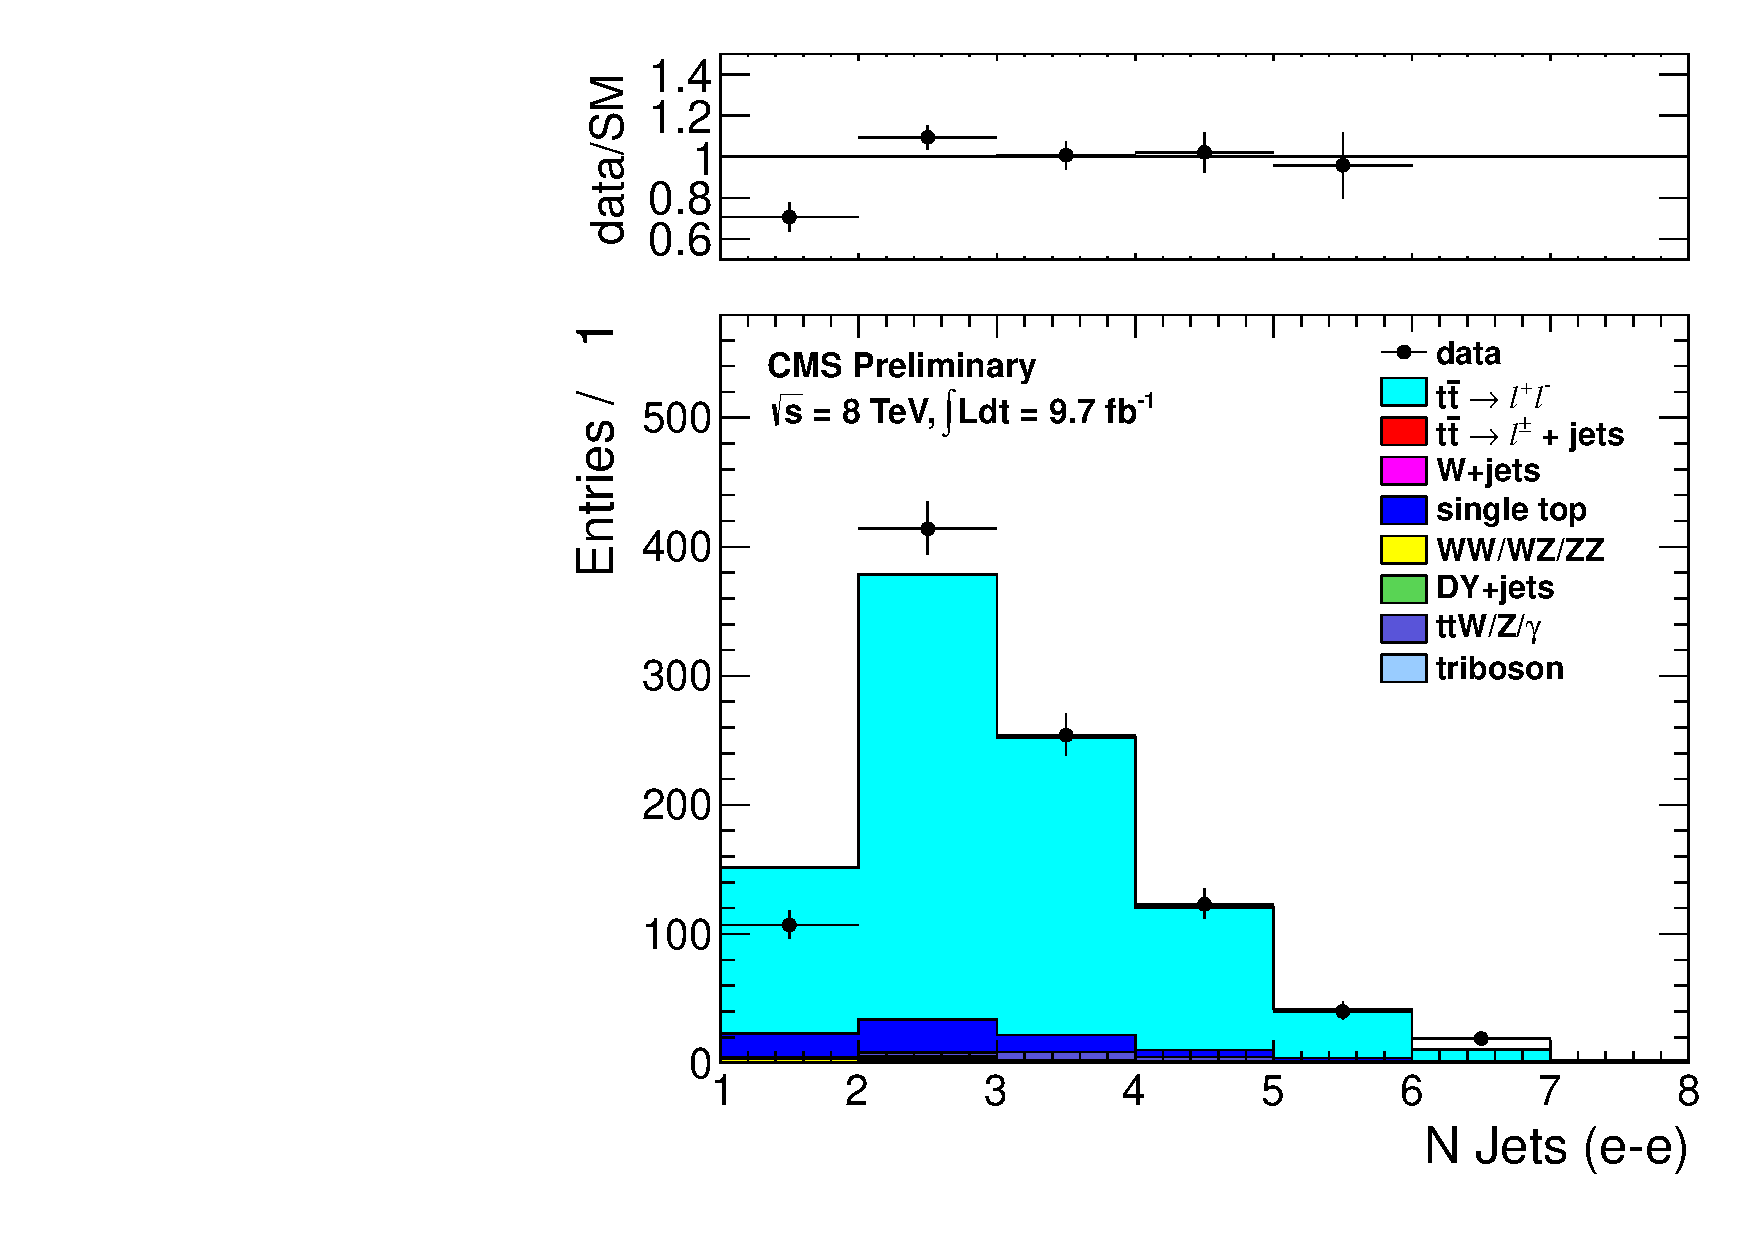
\includegraphics[width=0.5\linewidth]{plots/njets_all_met100_diel.pdf}%
        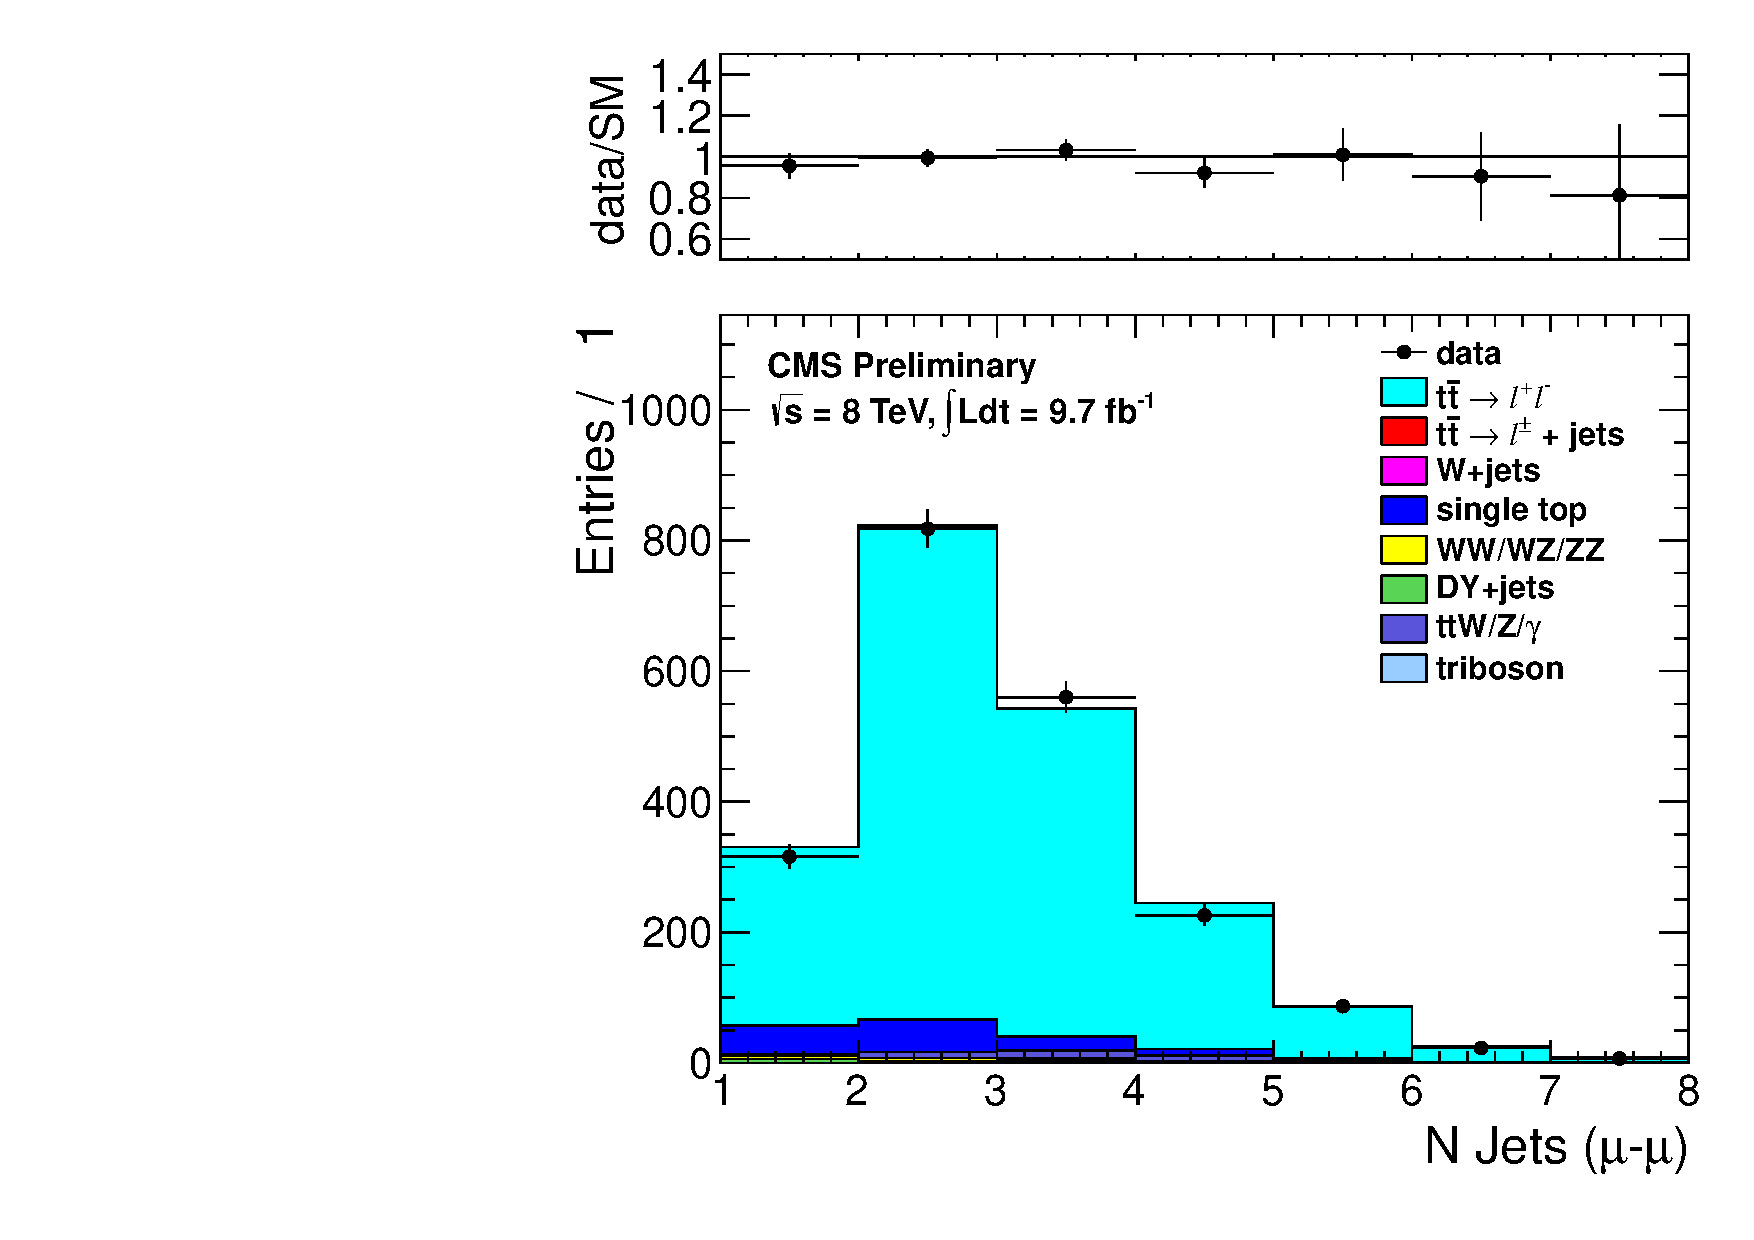
\includegraphics[width=0.5\linewidth]{plots/njets_all_met100_dimu.pdf}
	\caption{
	  \label{fig:dileptonnjets}%\protect 
          Comparison of the jet multiplicity distribution in data and MC for dilepton events in the \E-\M\
          (top), \E-\E\ (bottom left) and \M-\M\ (bottom right) channels.}  
      \end{center}
\end{figure}

It should be noted that in the case of \ttll\ events
with a single reconstructed lepton, the other lepton may be
mis-reconstructed as a jet. For example, a hadronic tau may be
mis-identified as a jet (since no $\tau$ identification is used). 
In this case only 1 additional jet from radiation may suffice for 
a \ttll\ event to enter the signal sample. As a result, both the
samples with $\ttbar+1$ jet and $\ttbar+\ge2$ jets are relevant for
estimating the top dilepton background in the signal region.

%In this section we discuss a correction to $ N_{2 lep}^{MC} $ in Equation XXX
%due to differences in the modelling of the jet multiplicity in data versus MC.
%The same correction also enters $ N_{peak}^{MC}$ in Equation XXX to the extend that the 
%dilepton contributions to $ N_{peak}^{MC}$ gets corrected.

%The dilepton control sample is defined by the following requirements:
%\begin{itemize}
%\item Exactly 2 selected electrons or muons with \pt $>$ 20 GeV
%\item \met\ $>$ 50 GeV
%\item $\geq1$ b-tagged jet
%\end{itemize}
%
%This sample is dominated by \ttll. The distribution of \njets\ for data and MC passing this selection is displayed in Fig.~\ref{fig:dilepton_njets}. 
%We use this distribution to derive scale factors which reweight the \ttll\ MC \njets\ distribution to match the data. We define the following
%quantities
%
%\begin{itemize}
%\item $N_{2}=$ data yield minus non-dilepton \ttbar\ MC yield for \njets\ $\leq$ 2
%\item $N_{3}=$ data yield minus non-dilepton \ttbar\ MC yield for \njets\ = 3
%\item $N_{4}=$ data yield minus non-dilepton \ttbar\ MC yield for \njets\ $\geq$ 4
%\item $M_{2}=$ dilepton \ttbar\ MC yield for \njets\ $\leq$ 2
%\item $M_{3}=$ dilepton \ttbar\ MC yield for \njets\ = 3
%\item $M_{4}=$ dilepton \ttbar\ MC yield for \njets\ $\geq$ 4
%\end{itemize}
%
%We use these yields to define 3 scale factors, which quantify the data/MC ratio in the 3 \njets\ bins:
%
%\begin{itemize}
%\item $SF_2 = N_2 / M_2$
%\item $SF_3 = N_3 / M_3$
%\item $SF_4 = N_4 / M_4$
%\end{itemize}
%
%And finally, we define the scale factors $K_3$ and $K_4$:
%
%\begin{itemize}
%\item $K_3 = SF_3 / SF_2$
%\item $K_4 = SF_4 / SF_2$
%\end{itemize}
%
%The scale factor $K_3$ is extracted from dilepton \ttbar\ events with \njets = 3, which have exactly 1 ISR jet.
%The scale factor $K_4$ is extracted from dilepton \ttbar\ events with \njets $\geq$ 4, which have at least 2 ISR jets.
%Both of these scale factors are needed since dilepton \ttbar\ events which fall in our signal region (including
%the \njets $\geq$ 4 requirement) may require exactly 1 ISR jet, in the case that the second lepton is reconstructed
%as a jet, or at least 2 ISR jets, in the case that the second lepton is not reconstructed as a jet. These scale
%factors are applied to the dilepton \ttbar\ MC only. For a given MC event, we determine whether to use $K_3$ or $K_4$
%by counting the number of reconstructed jets in the event ($N_{\rm{jets}}^R$) , and subtracting off any reconstructed 
%jet which is matched to the second lepton at generator level ($N_{\rm{jets}}^\ell$); $N_{\rm{jets}}^{\rm{cor}} = N_{\rm{jets}}^R - N_{\rm{jets}}^\ell$.
%For events with $N_{\rm{jets}}^{\rm{cor}}=3$ the factor $K_3$ is applied, while for events with $N_{\rm{jets}}^{\rm{cor}}\geq4$ the factor $K_4$ is applied.
%For all subsequent steps, the scale factors $K_3$ and $K_4$ have been
%applied to the \ttll\ MC.


Table~\ref{tab:njetskfactors}  shows scale factors ($K_3$ and $K_4$)
used to correct the
fraction of events with additional jets in MC to the observed fraction
in data.   These scale factors are calculated from Fig.~\ref{fig:dileptonnjets} 
as follows:
\begin{itemize}
\item $N_{2}=$ data yield minus non-dilepton \ttbar\ MC yield for \njets\ $\leq$ 2
\item $N_{3}=$ data yield minus non-dilepton \ttbar\ MC yield for \njets\ = 3
\item $N_{4}=$ data yield minus non-dilepton \ttbar\ MC yield for \njets\ $\geq$ 4
\item $M_{2}=$ dilepton \ttbar\ MC yield for \njets\ $\leq$ 2
\item $M_{3}=$ dilepton \ttbar\ MC yield for \njets\ = 3
\item $M_{4}=$ dilepton \ttbar\ MC yield for \njets\ $\geq$ 4
\end{itemize}
\noindent then
\begin{itemize}
\item $SF_2 = N_2 / M_2$
\item $SF_3 = N_3 / M_3$
\item $SF_4 = N_4 / M_4$
\item $K_3 = SF_3 / SF_2$
\item $K_4 = SF_4 / SF_2$
\end{itemize}
\noindent This insures that $K_3 M_3/(M_2 + K_3 M_3 + K_4 M_4) = N_3 /
(N_2+N_3+N_4)$ and similarly for the $\geq 4$ jet bin.


The factors $K_3$ and $K_4$ are applied to the \ttll\ MC throughout the
entire analysis, i.e. 
whenever \ttll\ MC is used to estimate or subtract
a yield or distribution. 
%
In order to do so, it is first necessary to count the number of
additional jets from radiation and exclude leptons mis-identified as
jets. A jet is considered a mis-identified lepton if it is matched to a
generator-level second lepton with sufficient energy to satisfy the jet
\pt\ requirement ($\pt>30~\GeV$).   Then \ttll\ events that need two
radiation jets to enter our selection are scaled by $K_4$,
while those that only need one radiation jet  are scaled by $K_3$.

\begin{table}[!ht]
\begin{center}
\begin{tabular}{l|c}
\hline
            Jet Multiplicity Sample
            &                Data/MC Scale Factor \\
\hline
\hline
N jets $= 3$ (sensitive to $\ttbar+1$ extra jet from radiation)   &
$K_3 = 1.01 \pm 0.03$\\
N jets $\ge4$ (sensitive to $\ttbar+\ge2$ extra jets from radiation)
&       $K_4 = 0.93 \pm 0.04$\\
\hline
\end{tabular}
\caption{Data/MC scale factors used to account for differences in the
  fraction of events with additional hard jets from radiation in
  \ttll\ events. \label{tab:njetskfactors}}
\end{center}
\end{table}

\clearpage



\subsubsection{Validation of the ``Physics'' Modelling of the \ttdl\
  MC in CR4}
\label{sec:CR4-valid}

[THE TEXT IN THIS SUBSECTION IS ESSENTIALLY COMPLETE]

As mentioned above, $t\bar{t} \to $ dileptons where one of the leptons
is somehow lost constitutes the main background.
The object of this test is to validate the $M_T$ distribution of this
background by looking at the $M_T$ distribution of well identified
dilepton events.
We construct a transverse mass variable from the leading lepton and
the \met.  We distinguish between events with leading electrons and
leading muons.  

The $t\bar{t}$ MC is corrected using the $K_3$ and $K_4$ factors
from Section~\ref{sec:jetmultiplicity}.  It is also normalized to the 
total data yield separately for the \met\ requirements of signal
regions A, B, C, and D.  These normalization factors are listed
in Table~\ref{tab:cr4mtsf} and are close to unity.

The underlying \met\ and $M_T$ distributions are shown in 
Figures~\ref{fig:cr4met} and~\ref{fig:cr4mtrest}.  The data-MC agreement
is quite good.  Quantitatively, this is also shown in Table~\ref{tab:cr4yields}.


\begin{table}[!h]
\begin{center}
{\footnotesize
\begin{tabular}{l||c||c|c|c|c|c}
\hline
Sample              & CR4PRESEL & CR4A & CR4B & CR4C &
CR4D & CR4E\\
\hline
\hline
Muon Data/MC-SF 	  & $1.01 \pm 0.03$ & $0.96 \pm 0.04$ & $0.99 \pm 0.07$ & $1.05 \pm 0.13$ & $0.91 \pm 0.20$ & $1.10 \pm 0.34$ \\
\hline
\hline
Electron Data/MC-SF 	  & $0.99 \pm 0.03$ & $0.99 \pm 0.05$ & $0.91 \pm 0.08$ & $0.84 \pm 0.13$ & $0.70 \pm 0.18$ & $0.73 \pm 0.29$ \\
\hline
\end{tabular}}
\caption{ Data/MC scale factors for total yields, applied to compare
  the shapes of the distributions.
  The uncertainties are statistical only.
\label{tab:cr4mtsf}}
\end{center}
\end{table}


\begin{table}[!h]
\begin{center}
{\footnotesize
\begin{tabular}{l||c||c|c|c|c|c}
\hline
Sample              & CR4PRESEL & CR4A & CR4B & CR4C &
CR4D & CR4E\\
\hline
\hline
Muon MC 		  & $256 \pm 5$ & $152 \pm 4$ & $91 \pm 3$ & $26 \pm 2$ & $6 \pm 1$ & $4 \pm 1$ \\
Muon Data 		  & $251$ & $156$ & $98$ & $27$ & $8$ & $6$ \\
\hline
Muon Data/MC SF 	  & $0.98 \pm 0.07$ & $1.02 \pm 0.09$ & $1.08 \pm 0.12$ & $1.04 \pm 0.21$ & $1.29 \pm 0.48$ & $1.35 \pm 0.59$ \\
\hline
\hline
Electron MC 		  & $227 \pm 5$ & $139 \pm 4$ & $73 \pm 3$ & $21 \pm 1$ & $5 \pm 1$ & $2 \pm 0$ \\
Electron Data 		  & $219$ & $136$ & $72$ & $19$ & $2$ & $1$ \\
\hline
Electron Data/MC SF 	  & $0.96 \pm 0.07$ & $0.98 \pm 0.09$ & $0.99 \pm 0.12$ & $0.92 \pm 0.22$ & $0.41 \pm 0.29$ & $0.53 \pm 0.54$ \\
\hline
\end{tabular}}
\caption{ Yields in \mt\ tail comparing the MC prediction (after
  applying SFs) to data. The uncertainties are statistical only.
\label{tab:cr4yields}}
\end{center}
\end{table}

\begin{figure}[hbt]
  \begin{center}
        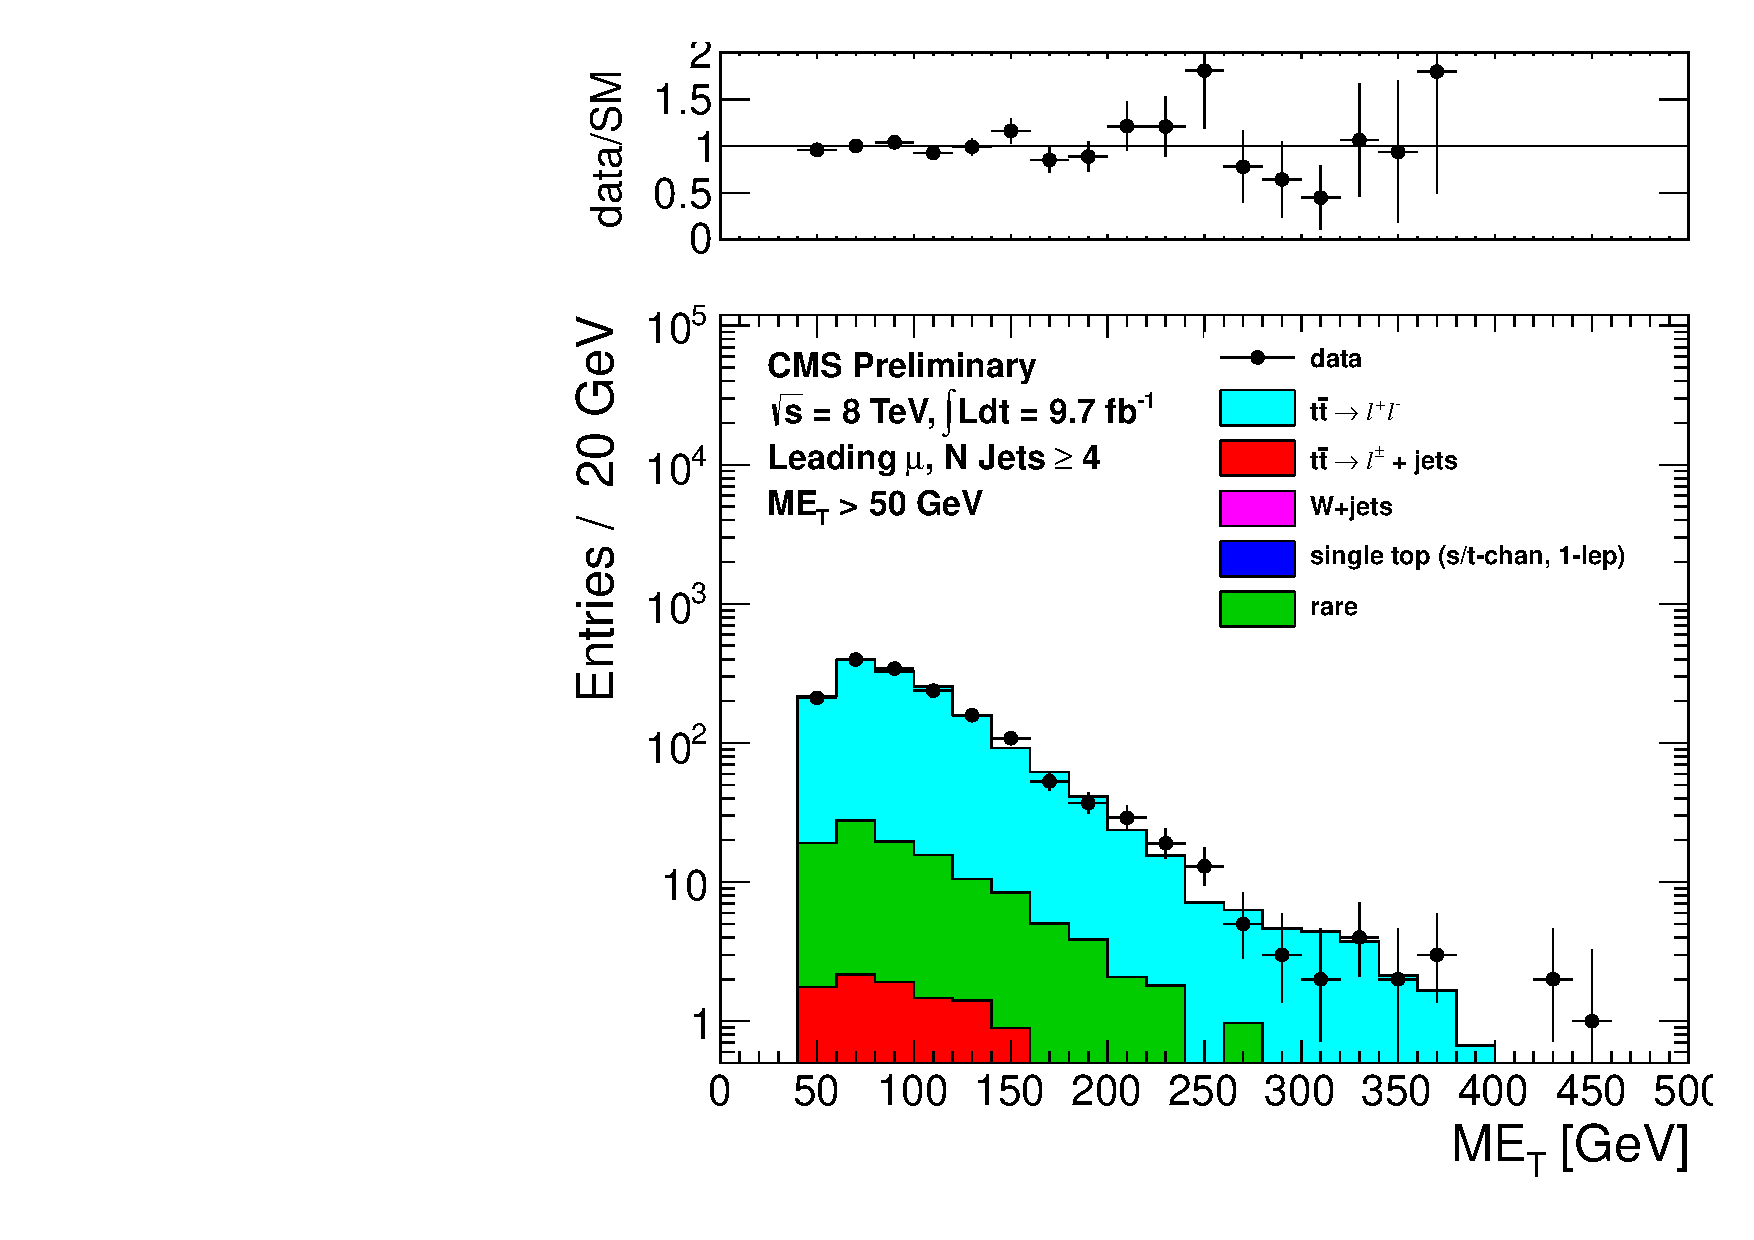
\includegraphics[width=0.5\linewidth]{plots/CR4plots/met_met50_leadmuo_nj4.pdf}%
        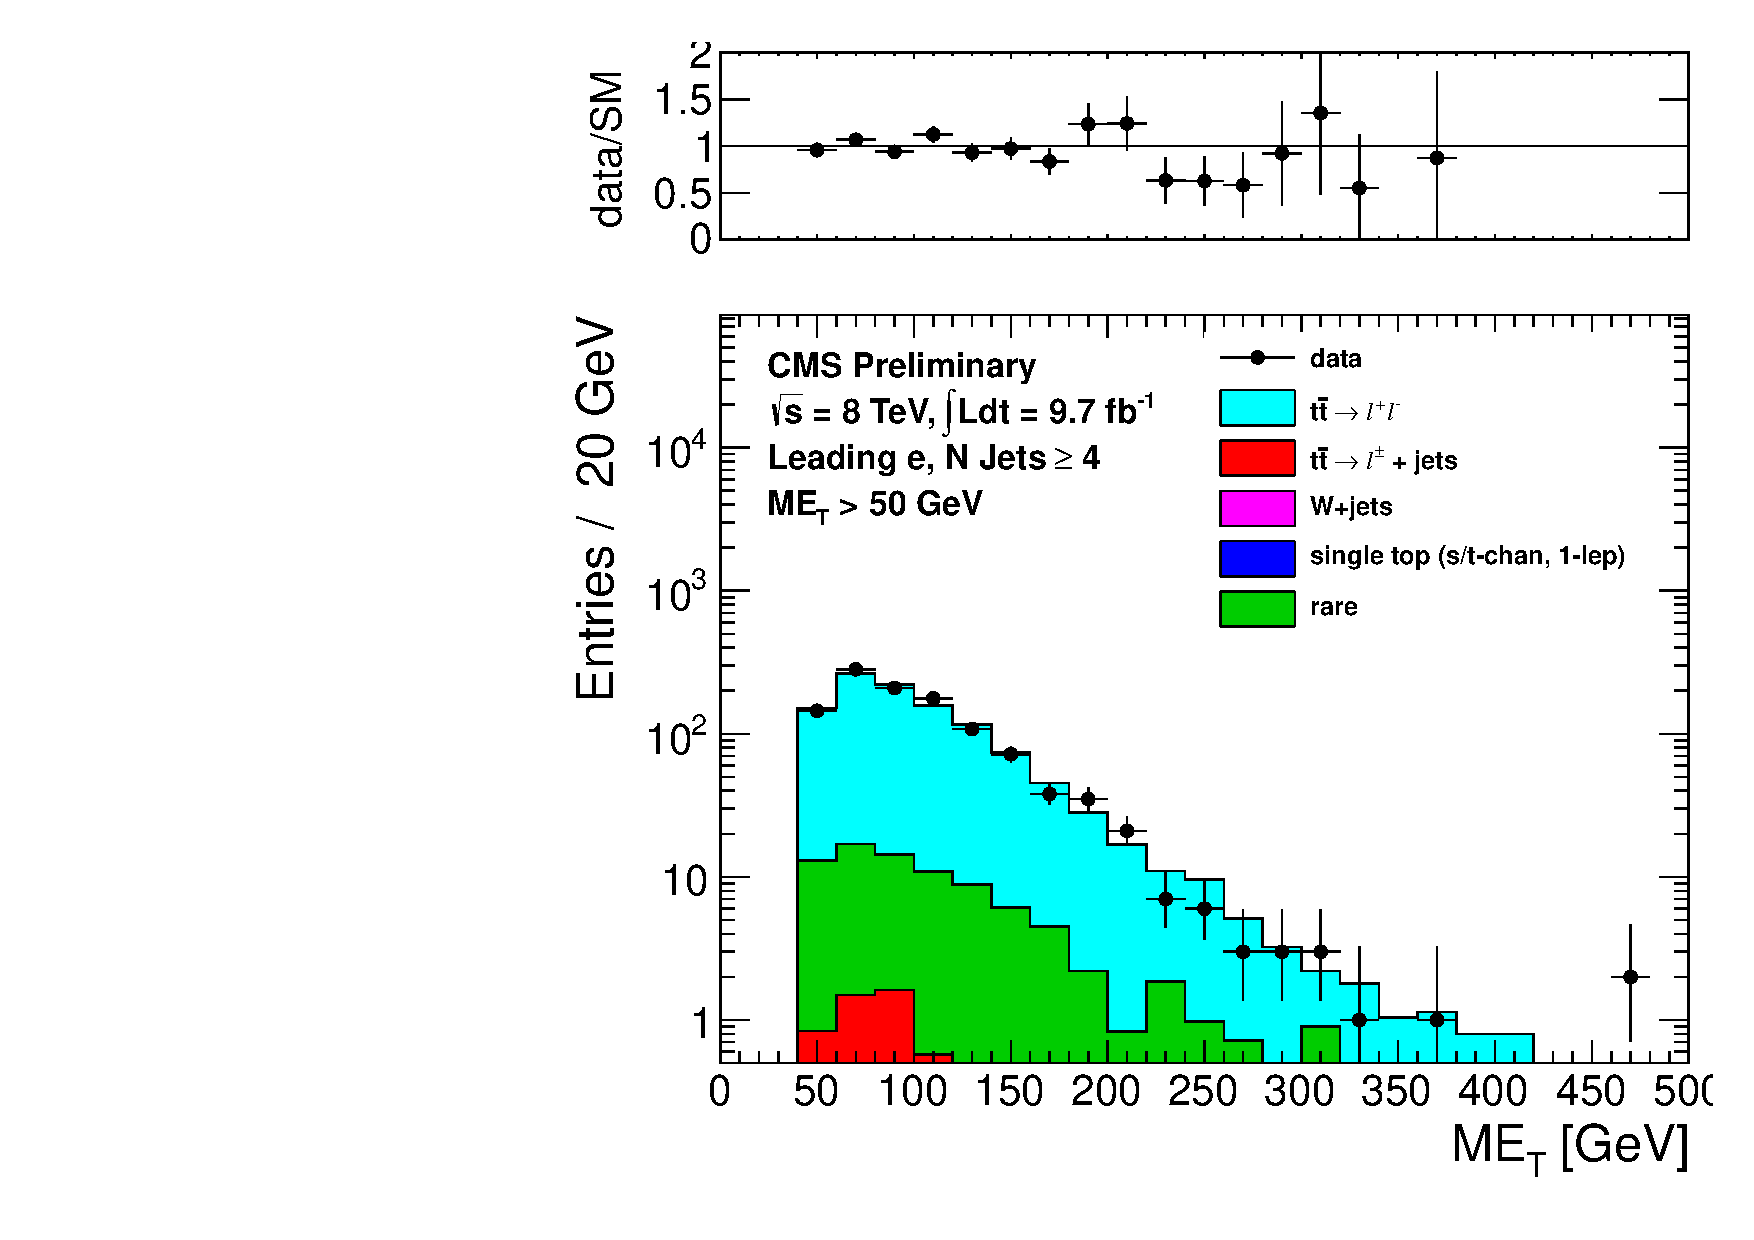
\includegraphics[width=0.5\linewidth]{plots/CR4plots/met_met50_leadele_nj4.pdf}
        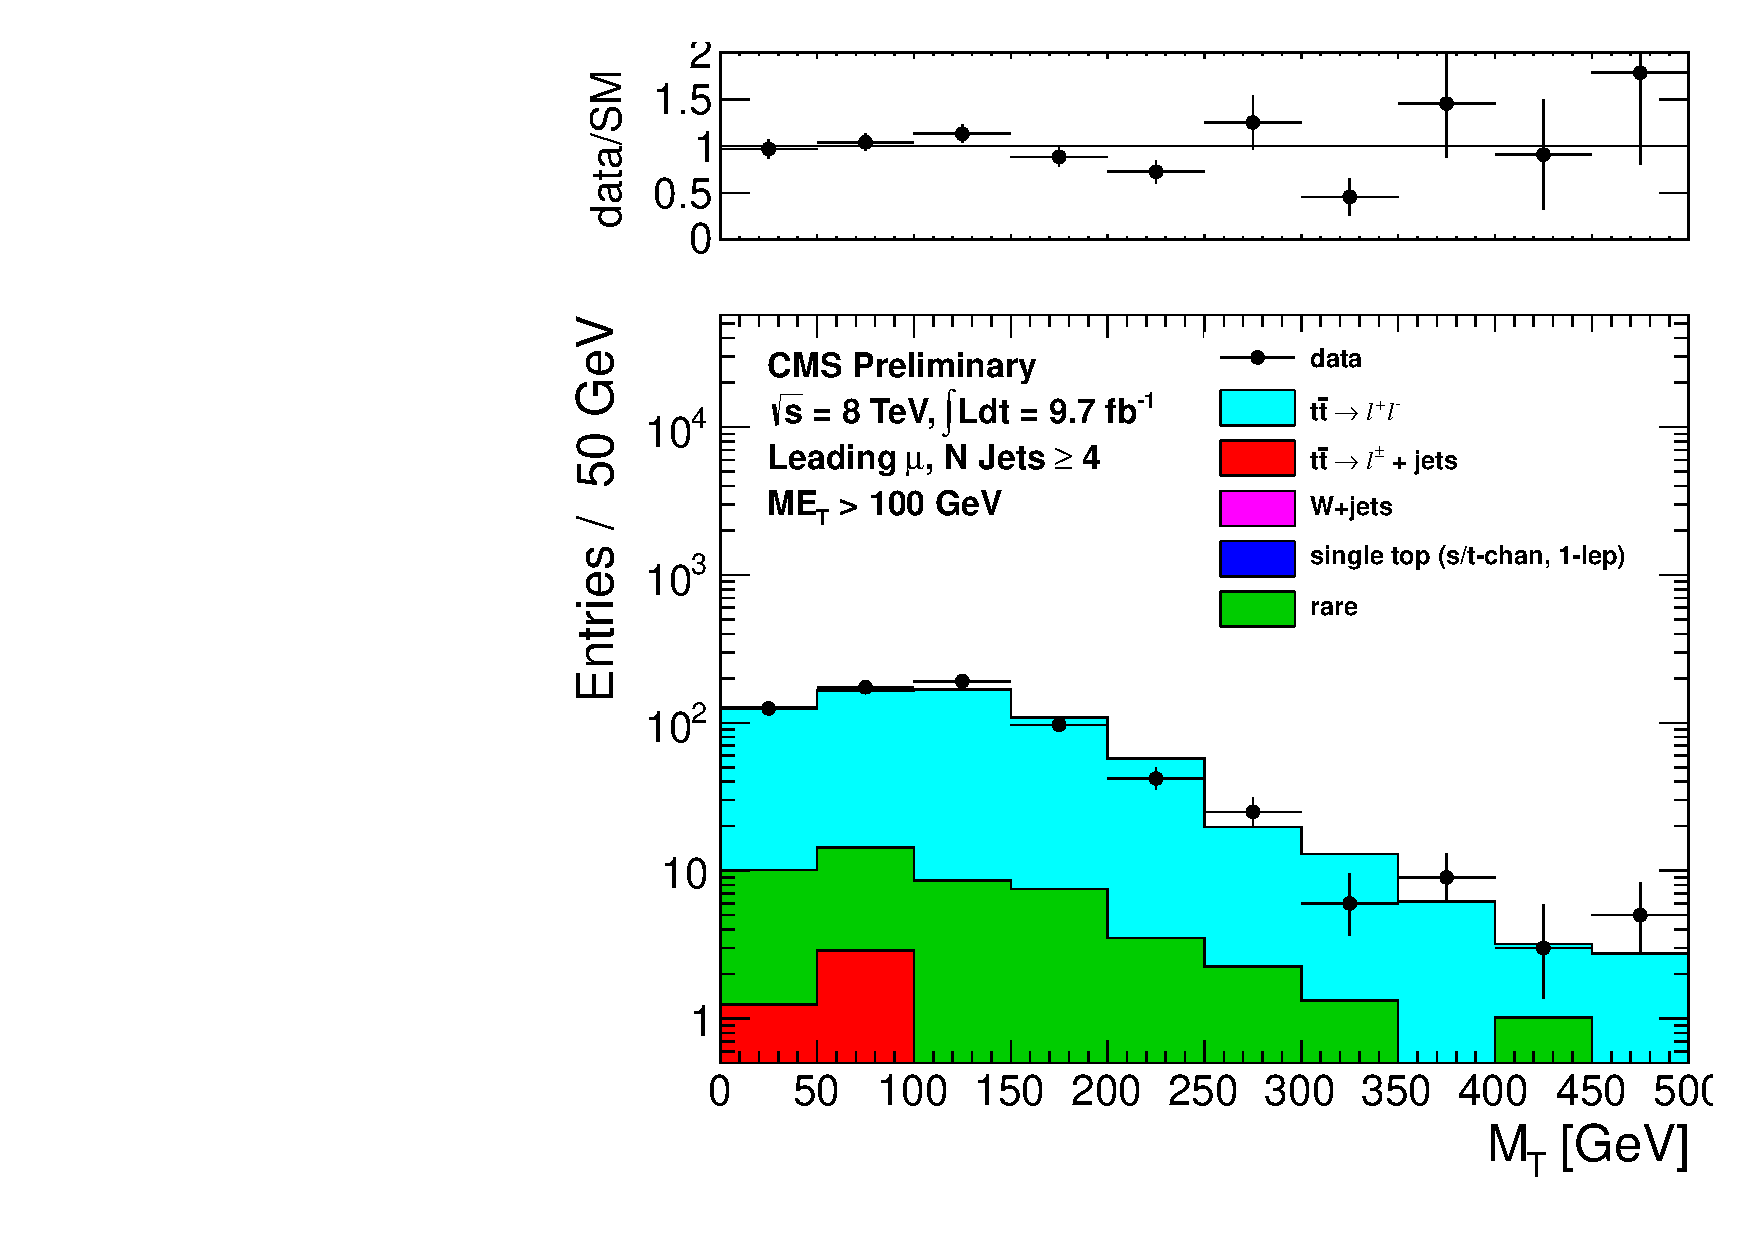
\includegraphics[width=0.5\linewidth]{plots/CR4plots/mt_met100_leadmuo_nj4.pdf}%
        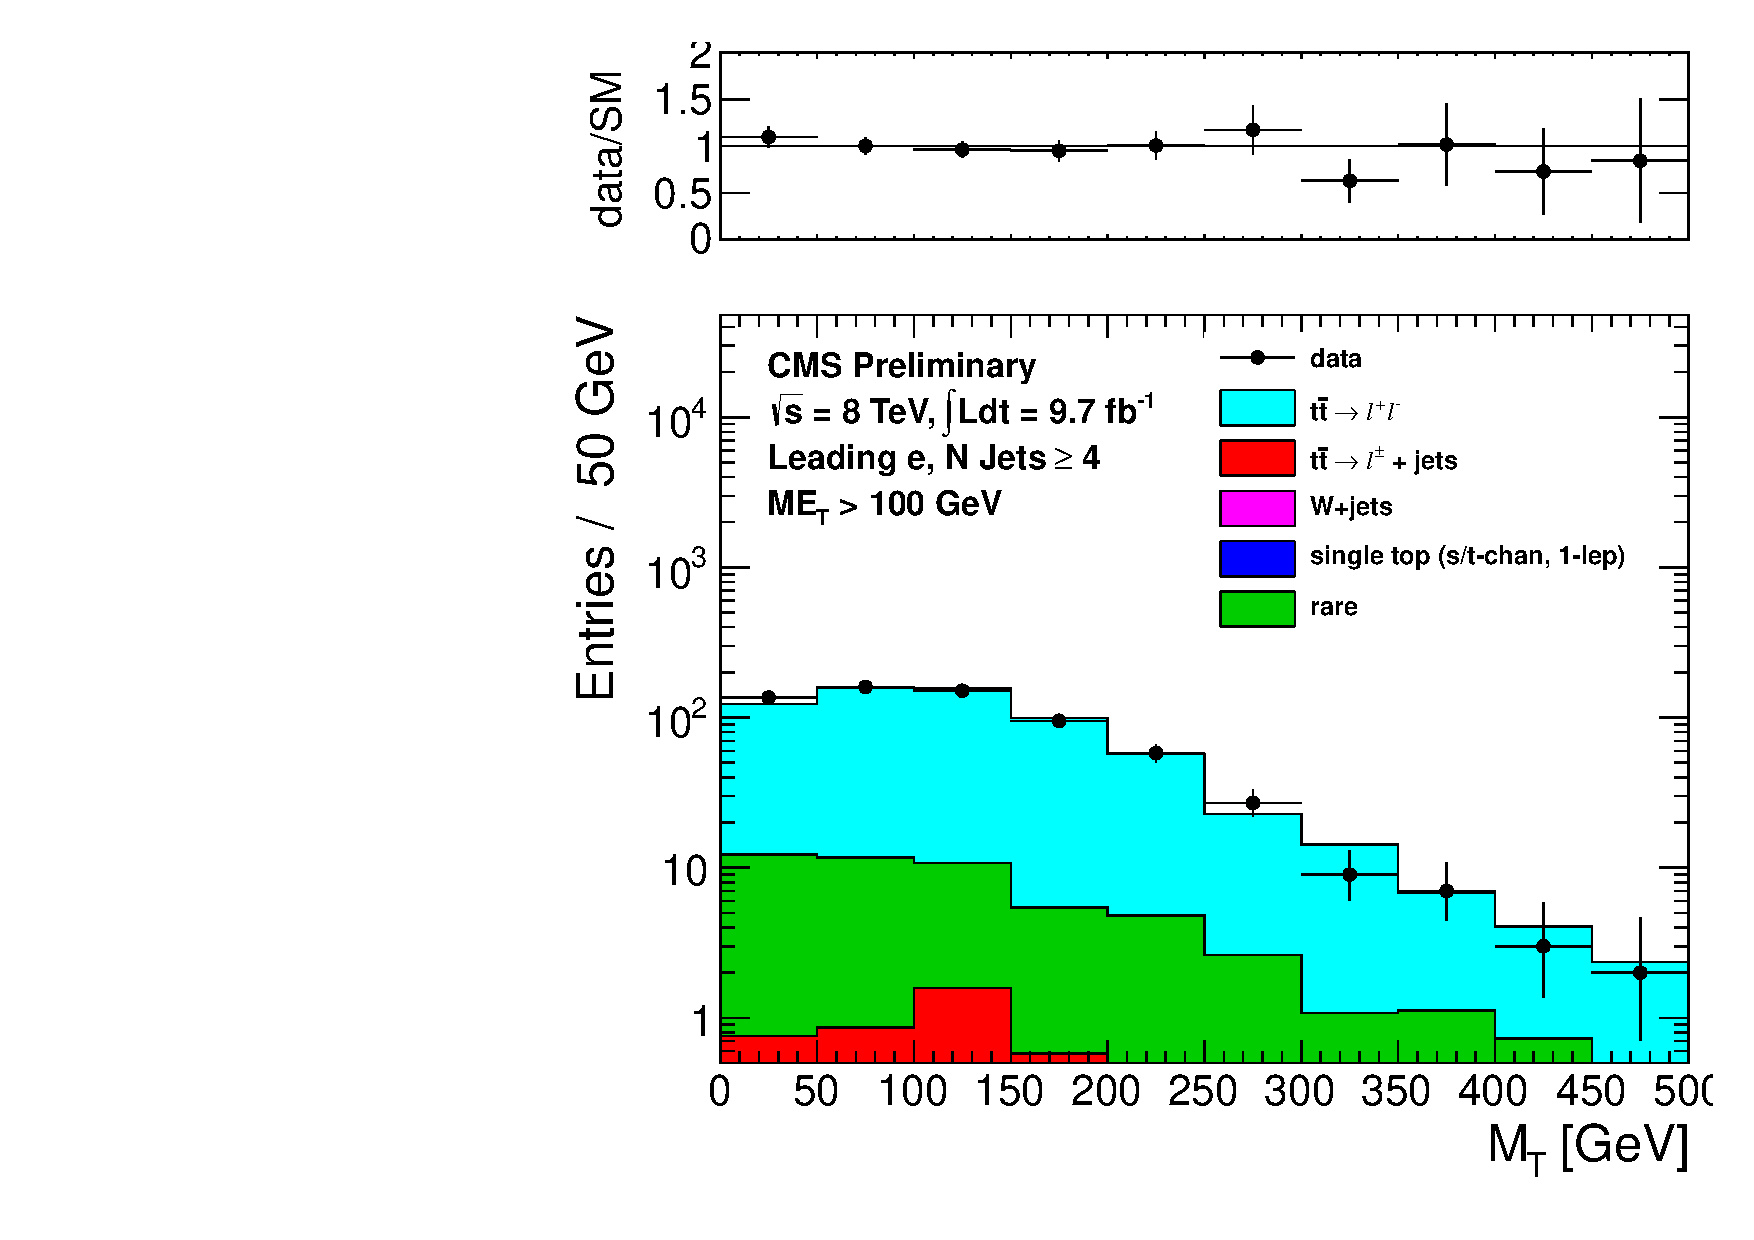
\includegraphics[width=0.5\linewidth]{plots/CR4plots/mt_met100_leadele_nj4.pdf}
    \caption{
      Comparison of the \met\ (top) and \mt\ for $\met>100$ (bottom) distributions in data vs. MC for events
      with a leading muon (left) and leading electron (right)
      satisfying the requirements of CR4. 
\label{fig:cr4met} 
}  
      \end{center}
\end{figure}

\begin{figure}[hbt]
  \begin{center}
        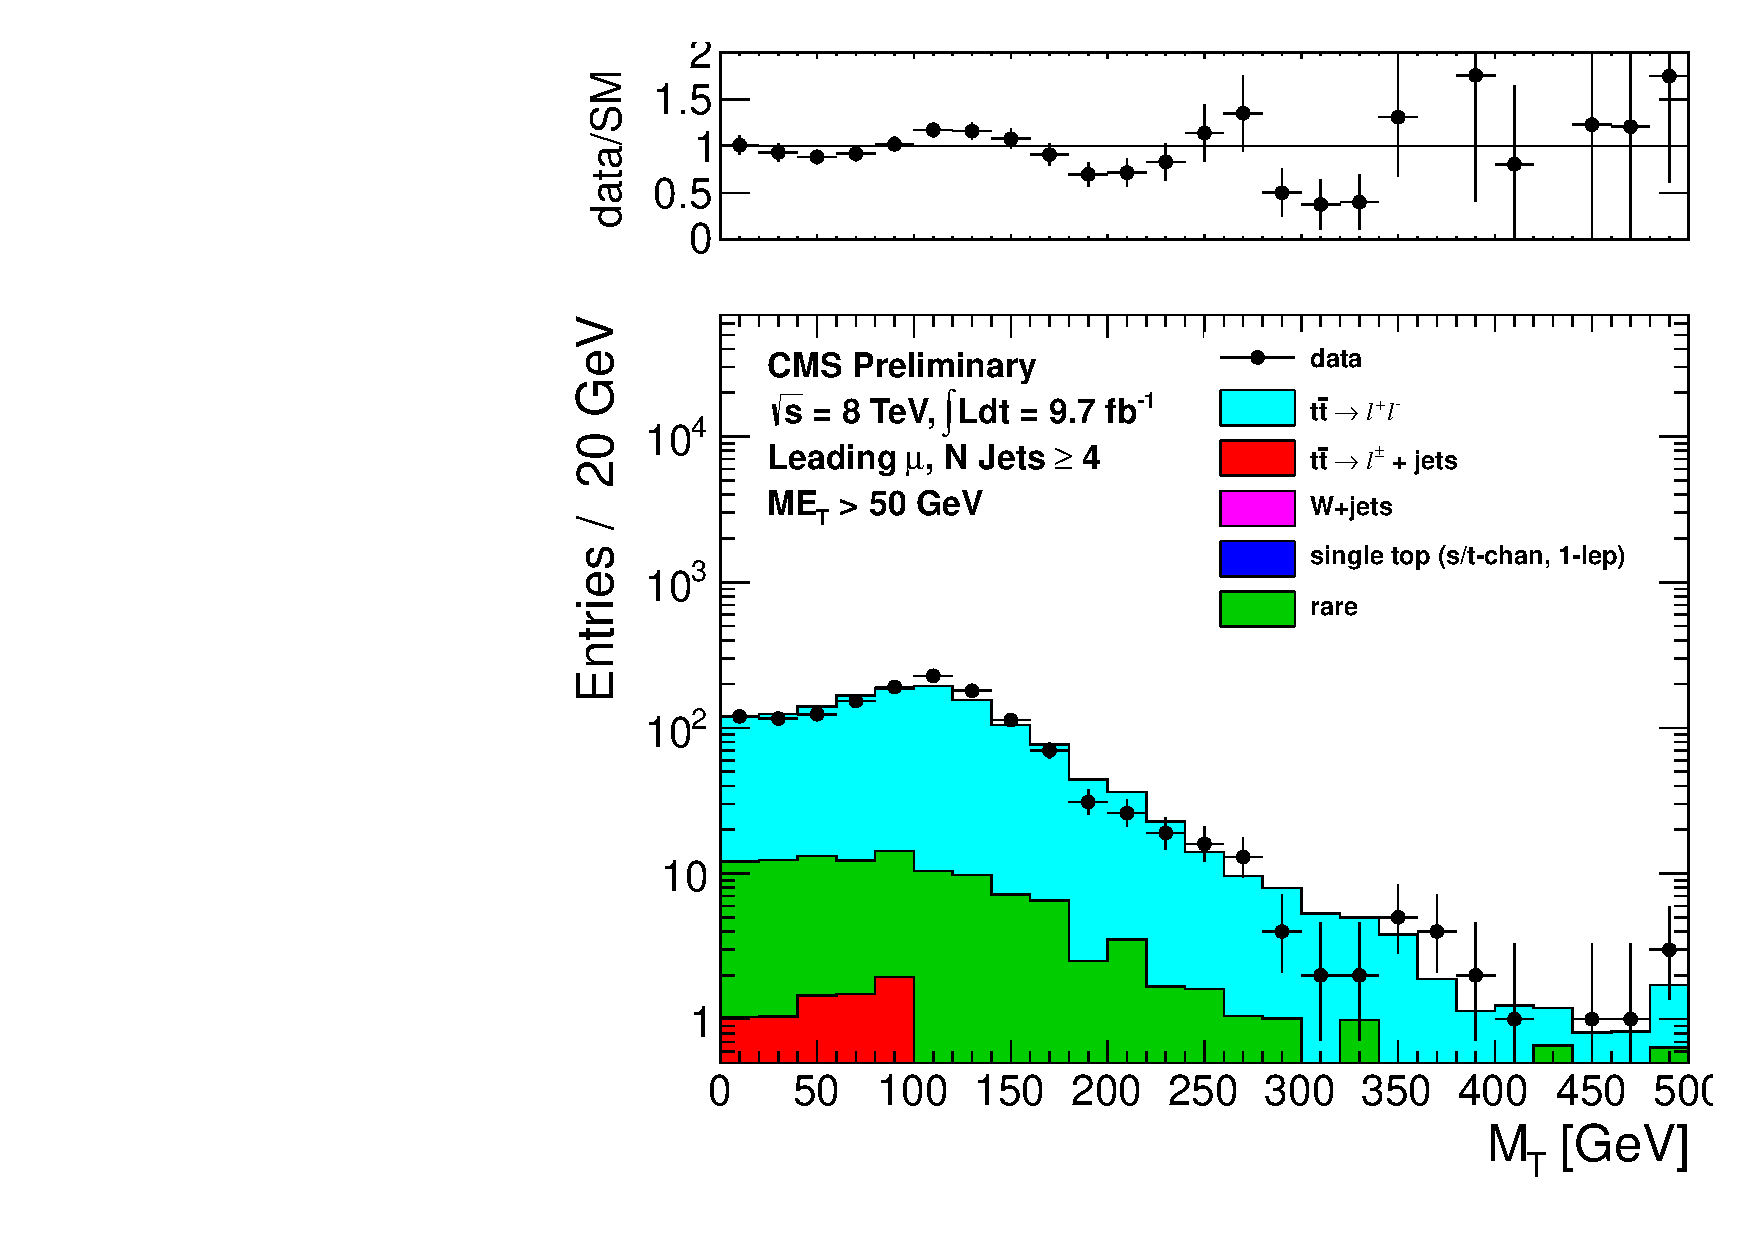
\includegraphics[width=0.5\linewidth]{plots/CR4plots/mt_met50_leadmuo_nj4.pdf}%
        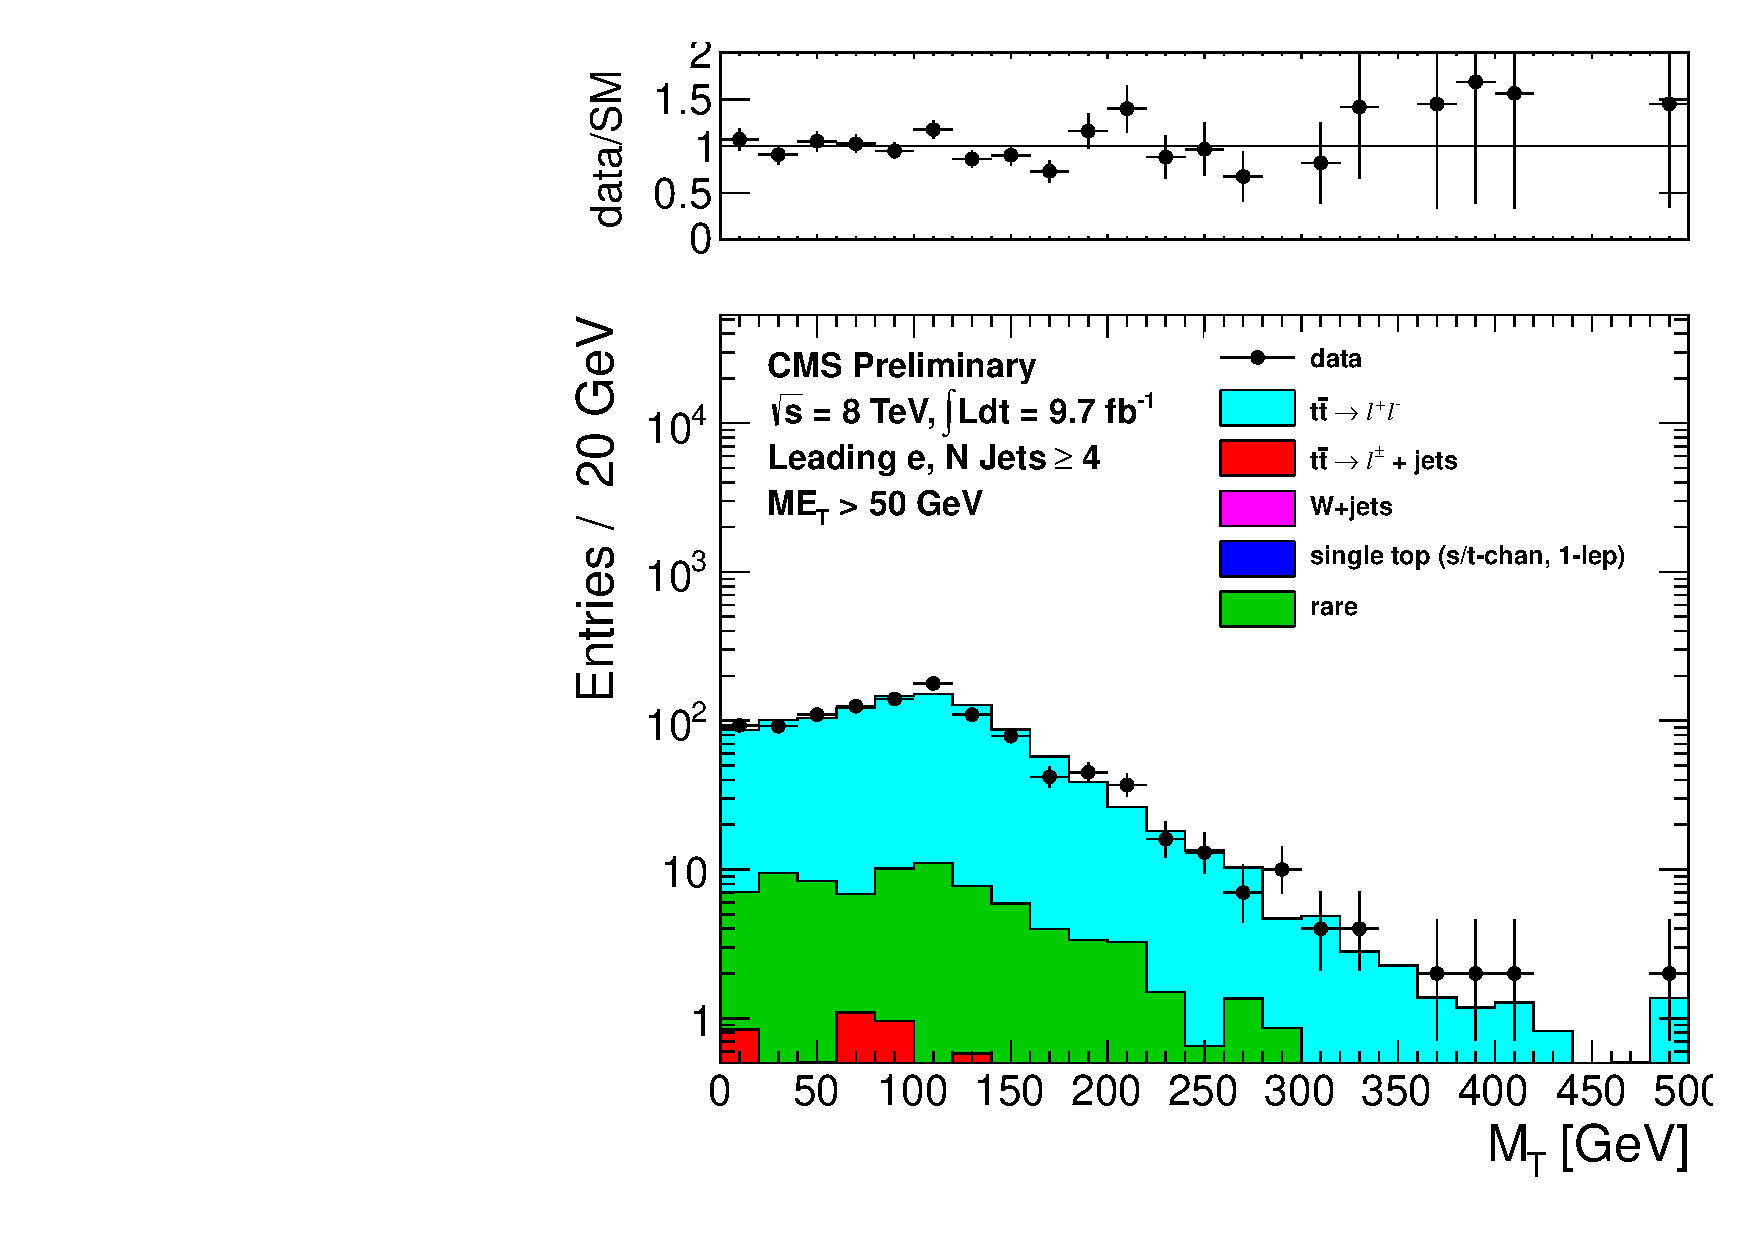
\includegraphics[width=0.5\linewidth]{plots/CR4plots/mt_met50_leadele_nj4.pdf}
        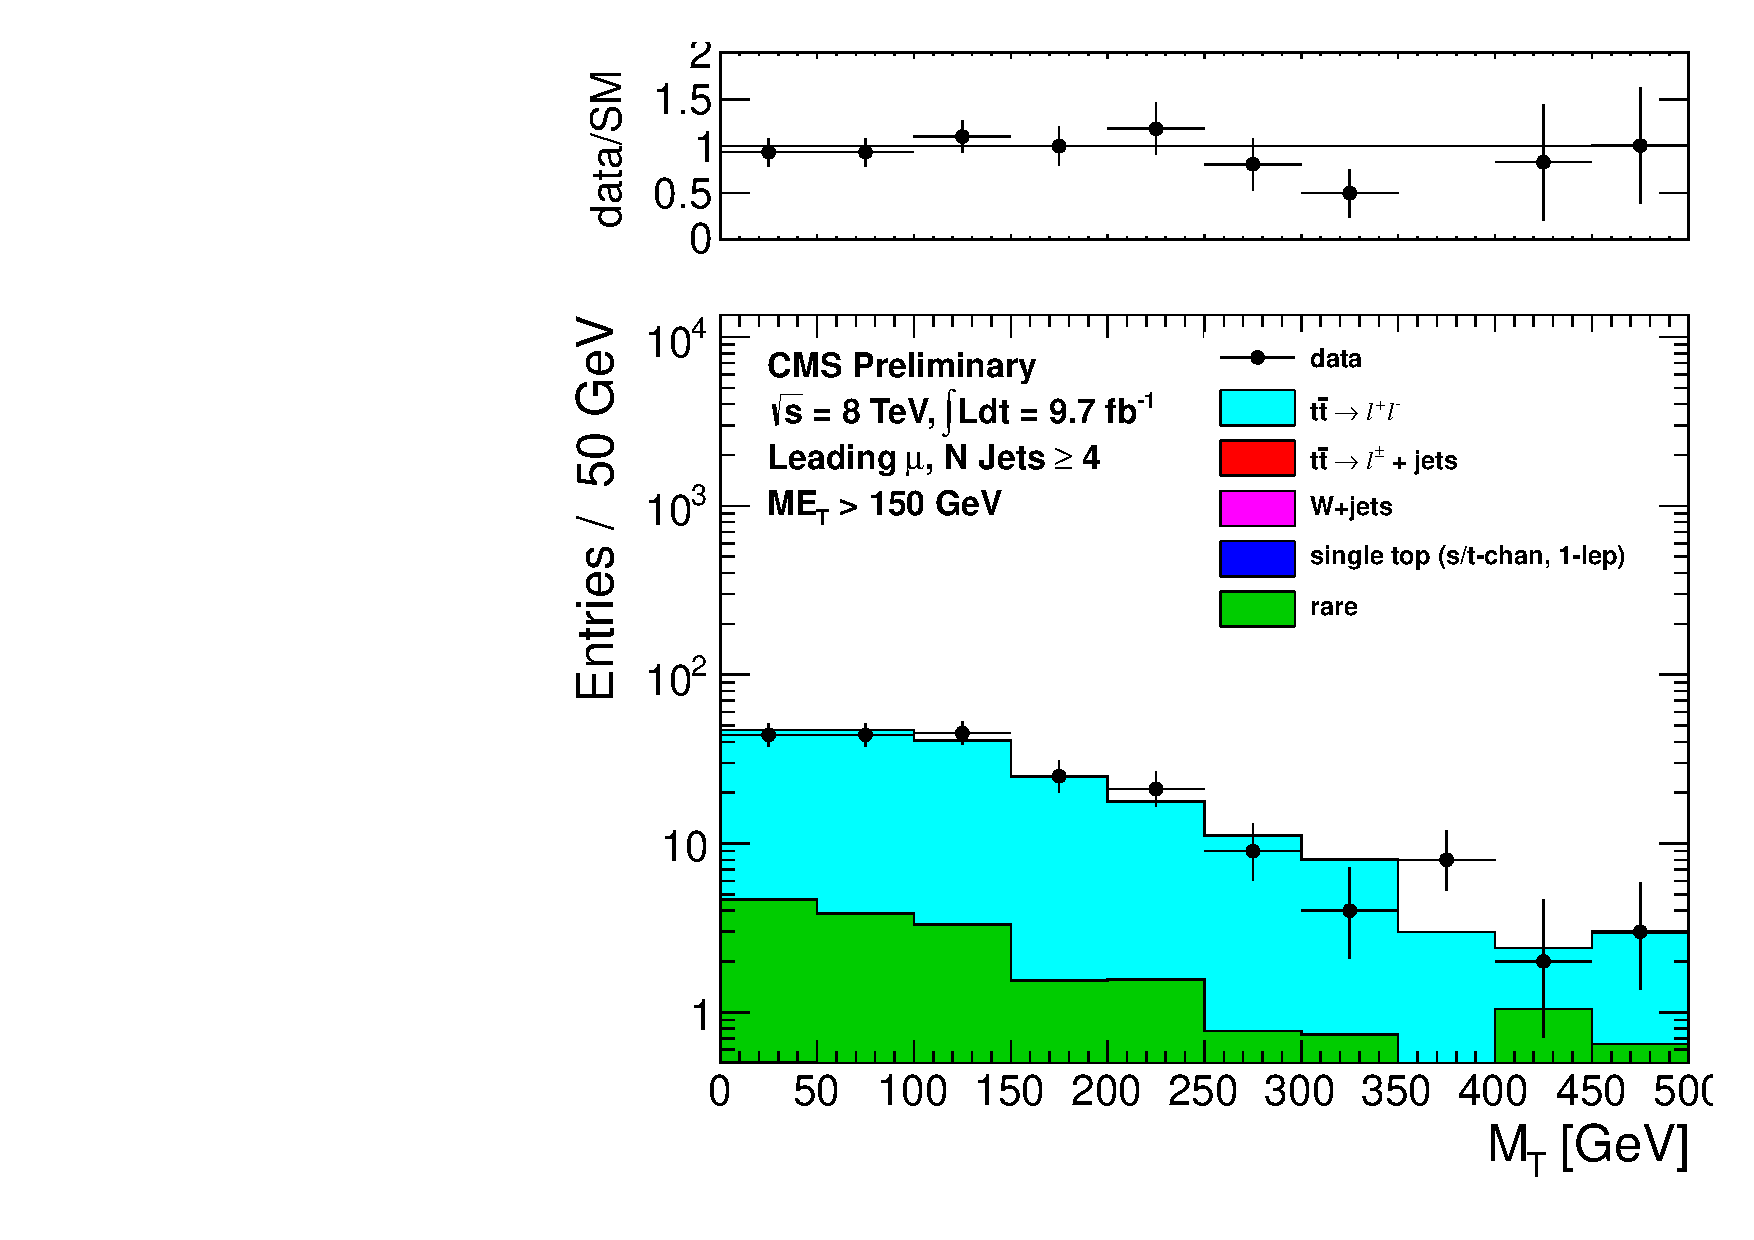
\includegraphics[width=0.5\linewidth]{plots/CR4plots/mt_met150_leadmuo_nj4.pdf}%
        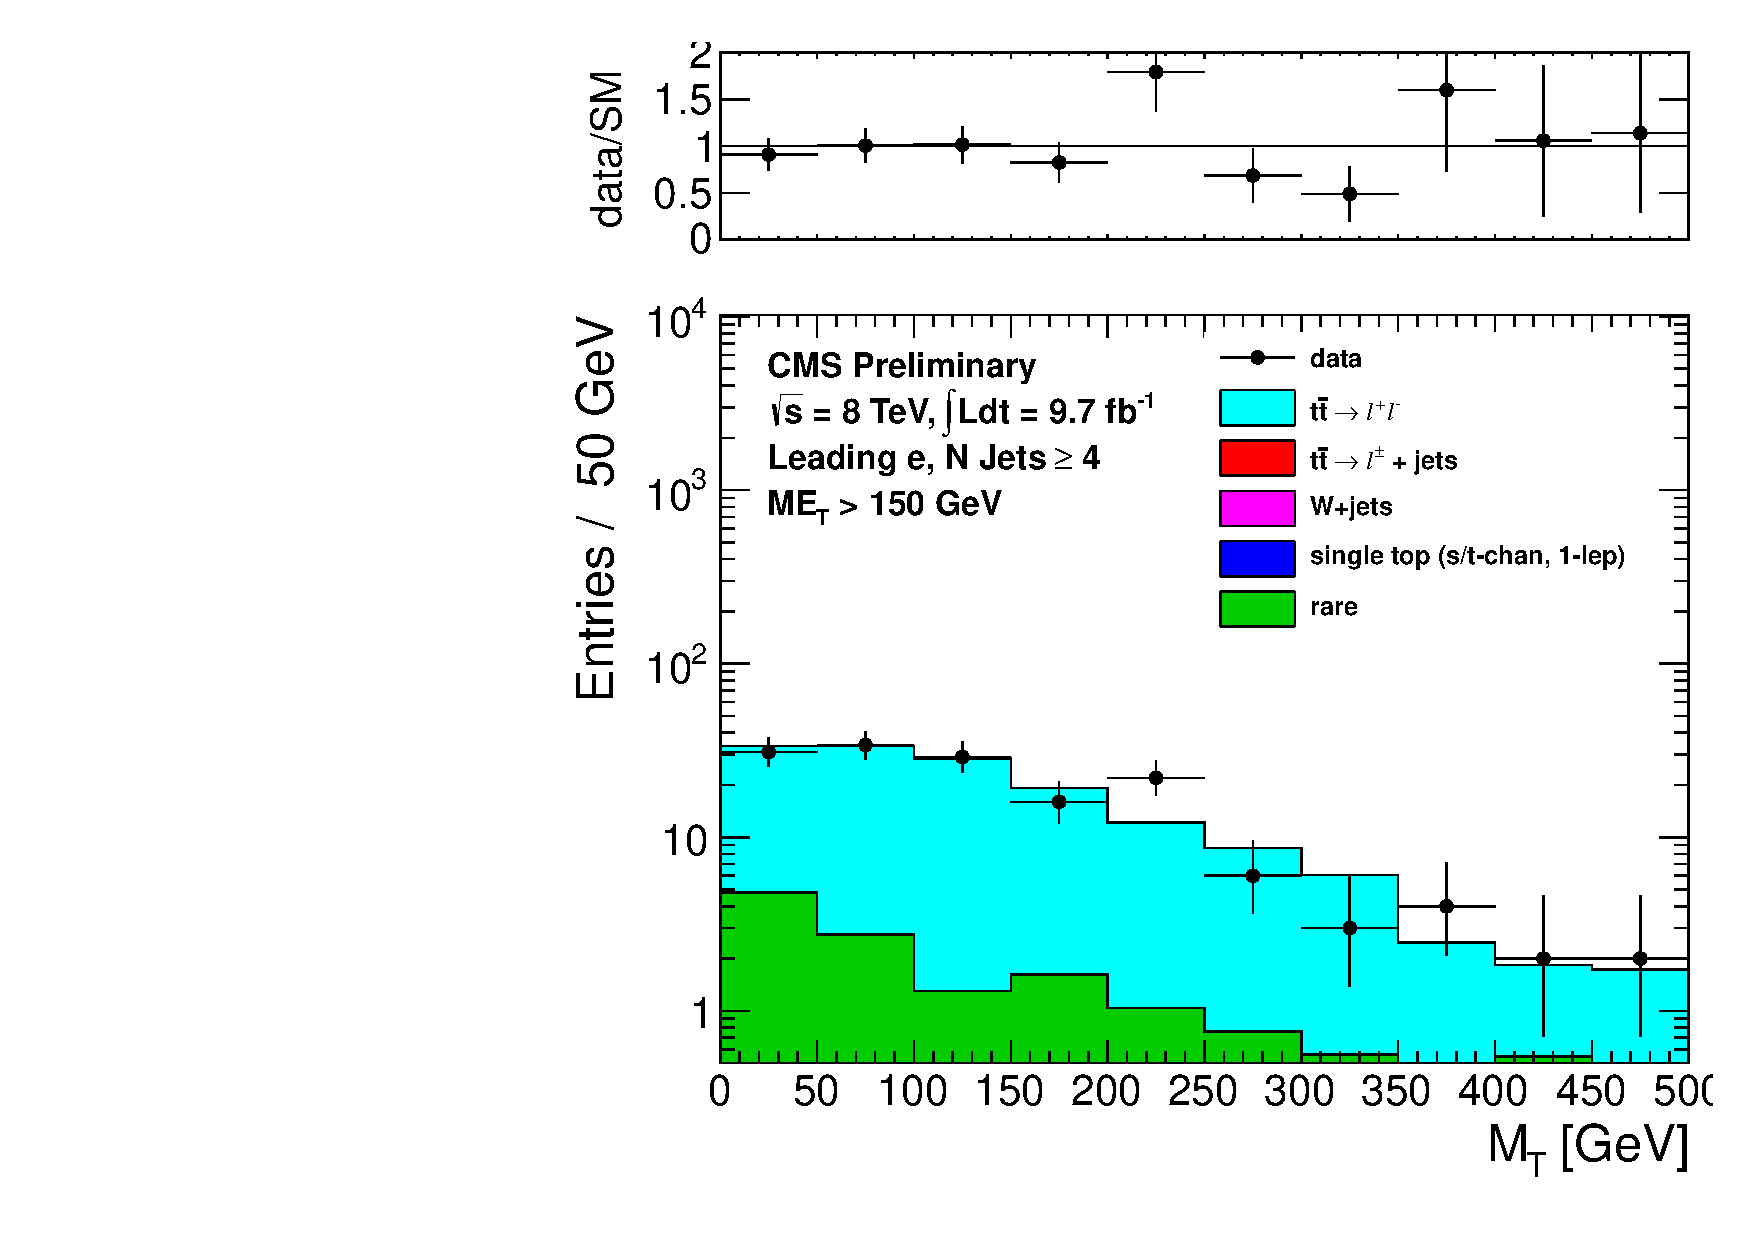
\includegraphics[width=0.5\linewidth]{plots/CR4plots/mt_met150_leadele_nj4.pdf}
        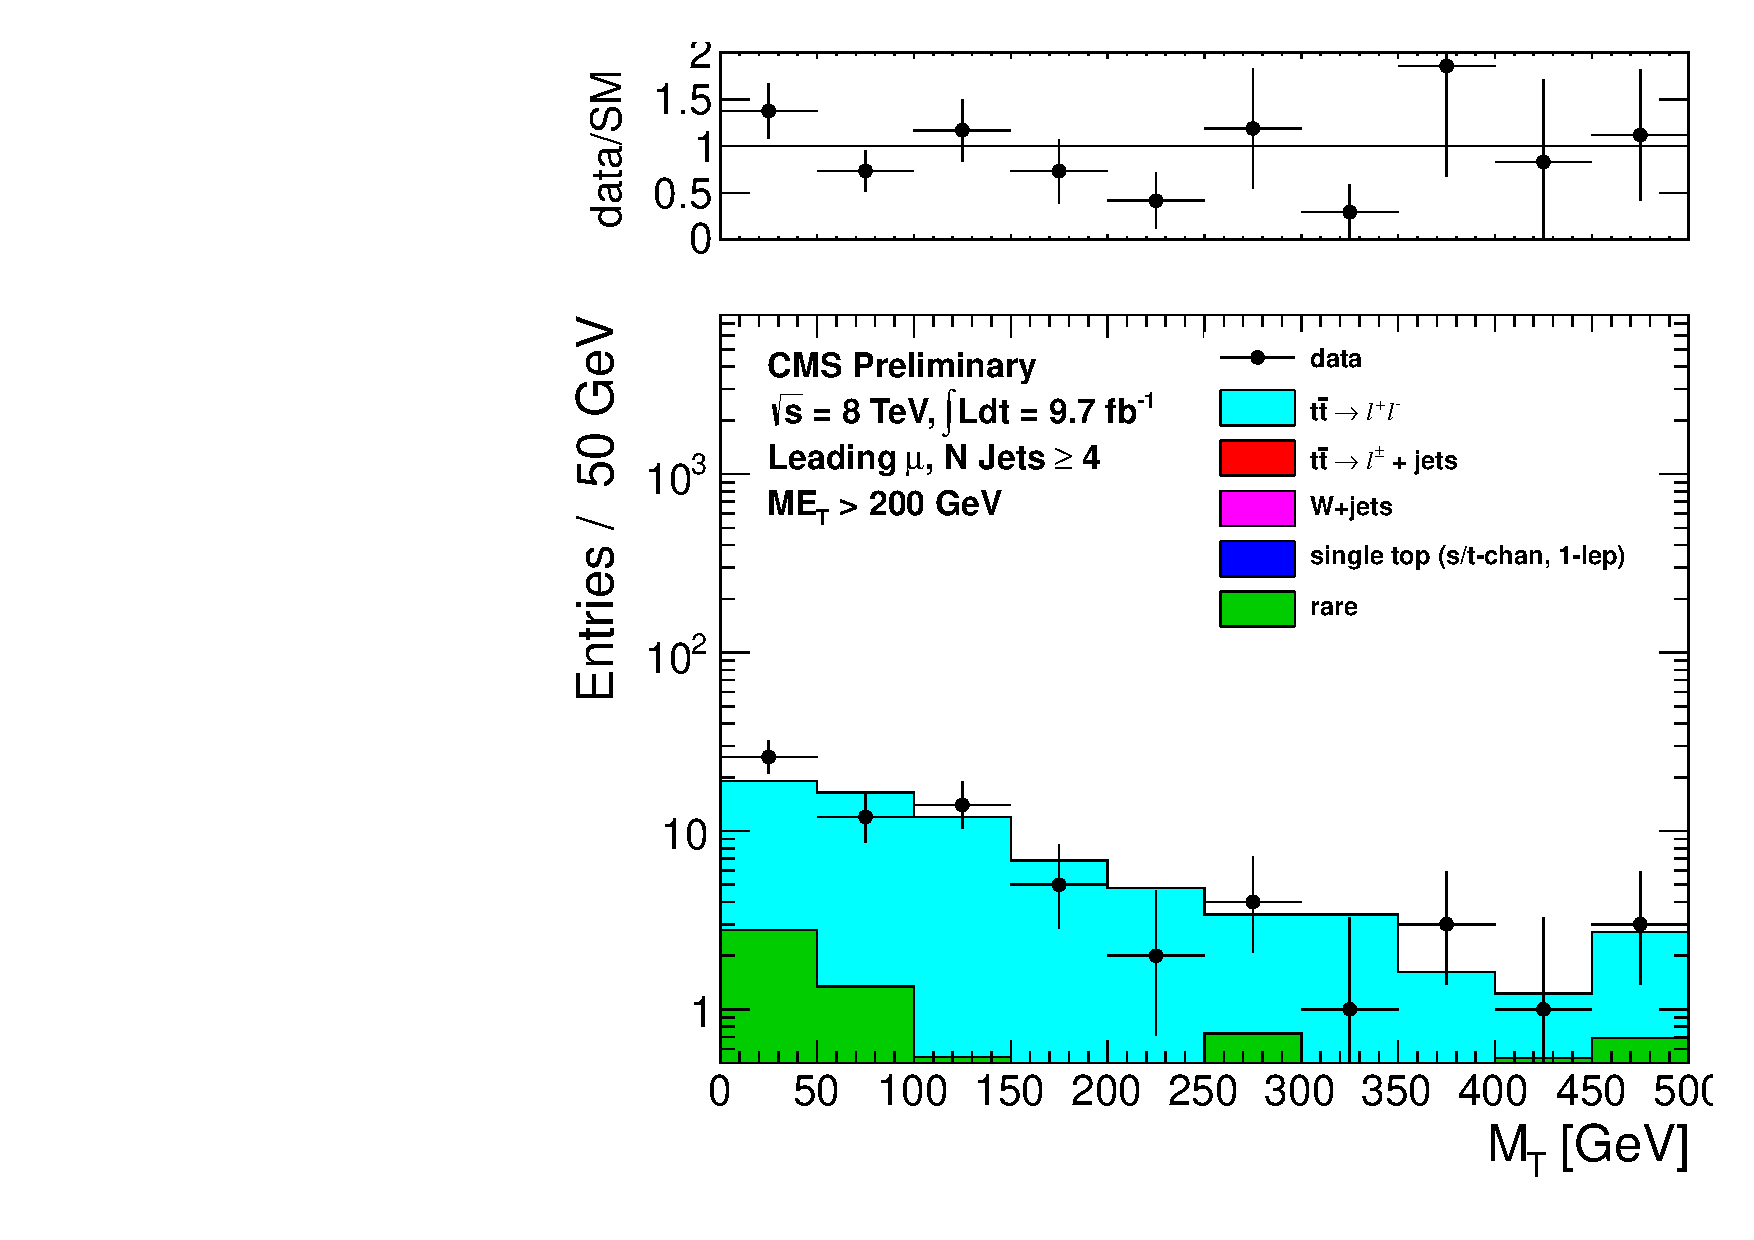
\includegraphics[width=0.5\linewidth]{plots/CR4plots/mt_met200_leadmuo_nj4.pdf}%
        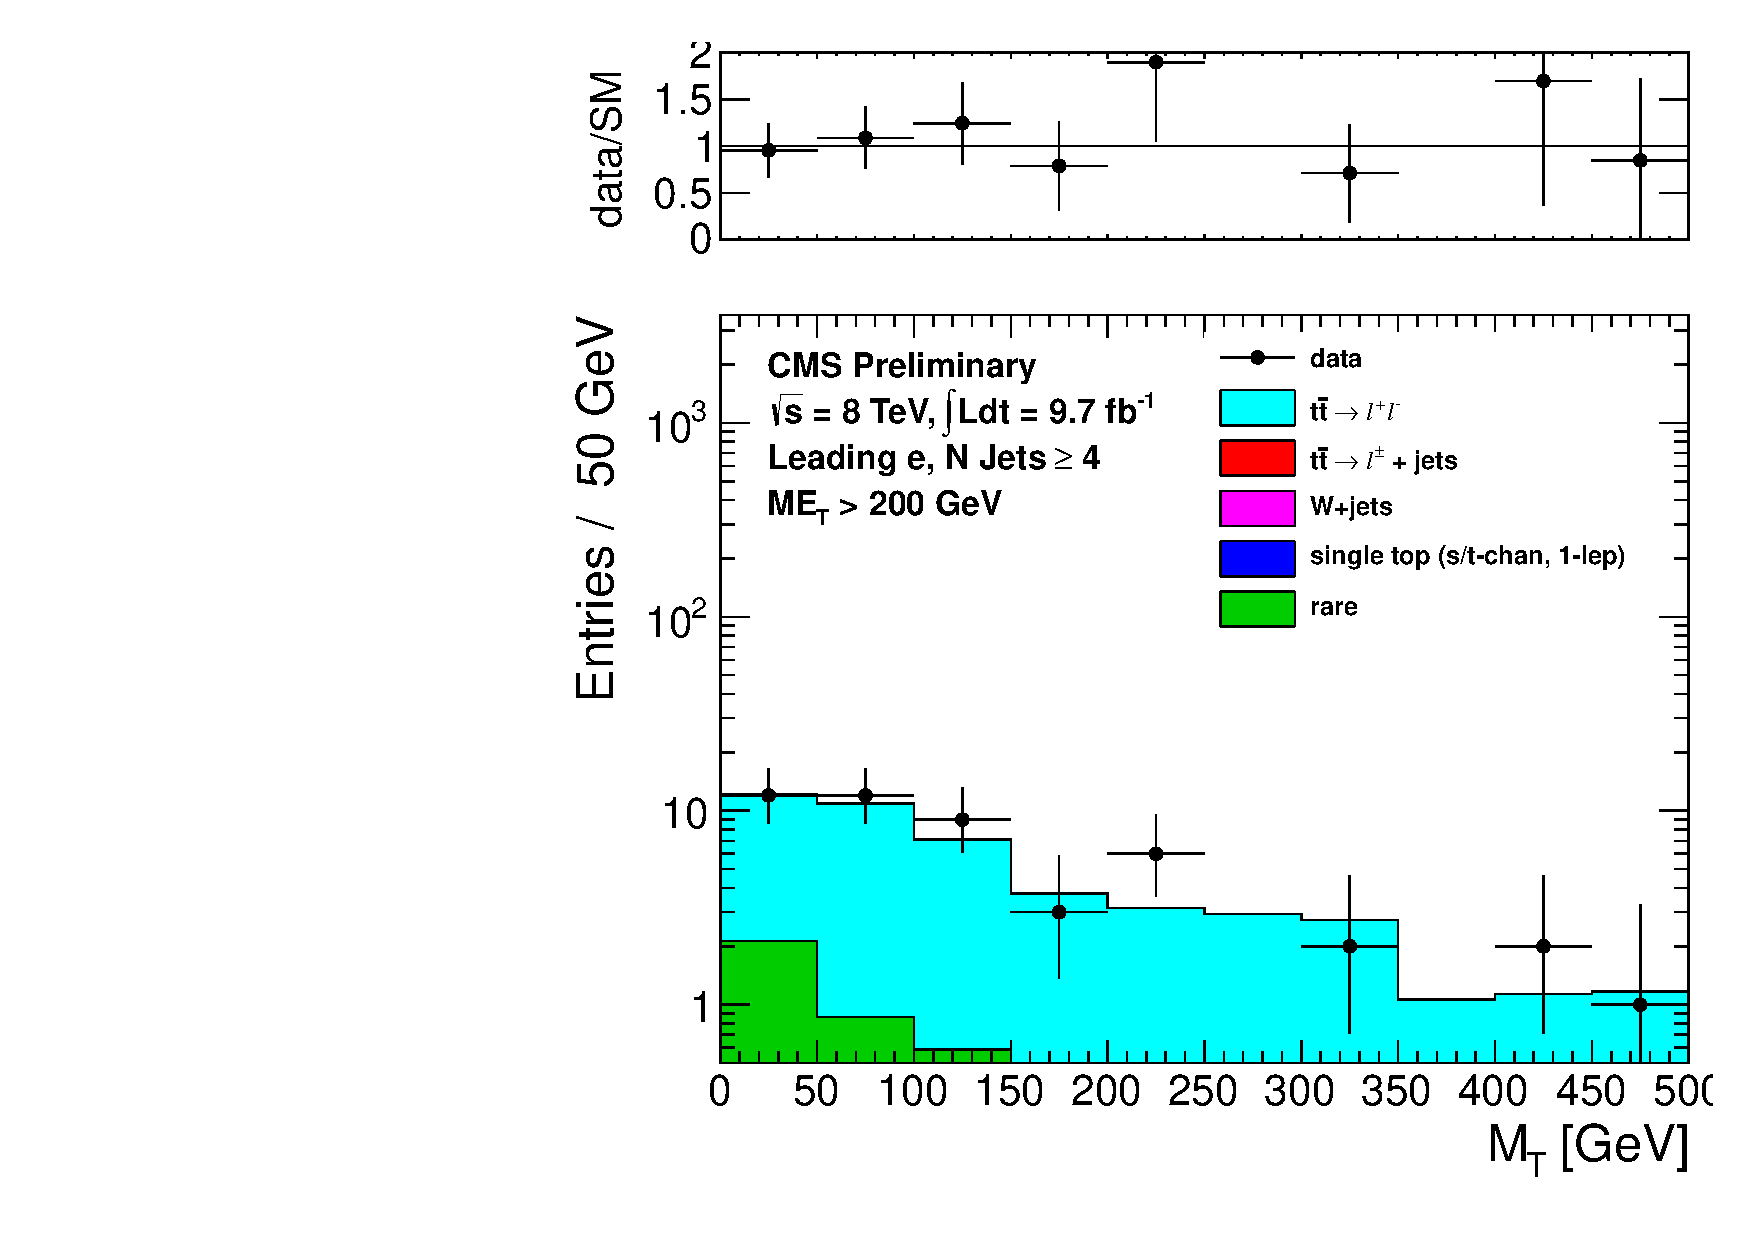
\includegraphics[width=0.5\linewidth]{plots/CR4plots/mt_met200_leadele_nj4.pdf}
    \caption{
      Comparison of the \mt\ distribution in data vs. MC for events
      with a leading muon (left) and leading electron (right)
      satisfying the requirements of CR4. The \met\ requirements used are
      50 GeV (top), 200 GeV (middle) and 250 GeV (bottom).
\label{fig:cr4mtrest} 
}  
      \end{center}
\end{figure}


\clearpage

\subsection{Test of control region with isolated track in CR5}
\label{sec:CR5}

[NEED TO VERIFY THAT THE DESCRIPTION OF SCALE FACTORS IS CORRECT AND
ADD A LITTLE BIT OF DETAIL, AS NOTED IN THE TEXT]

This CR consists of events that pass all cuts but fail the isolated
track veto cut.  These events (especially in the tail of $M_T$) are 
predominantly $t\bar{t}$ dileptons.  Thus the test in this control
regions is similar to that performed in CR4 and described
in Section~\ref{sec:CR4-valid}.  There is some non-trivial 
complementarity because CR5 also includes events with 
taus and events with electrons or muons below the threshold of
the CR4 selection.  Also, this test is somewhat sensitive to
the simulation of the track isolation requirement, since the
number of dilepton events in CR5 depends on the (in)efficiency 
of that cut.



In CR5 there is also a significant component
of $t\bar{t} \to \ell +$ jets, where one of the jets fluctuates
to an isolated track.  This component dominates at low $M_T$
and is not necessarily well reproduced quantitatively by the 
simulation.  This makes the normalization of the top MC a little bit tricky.
We define a ``pre-veto'' sample as the sample of events that pass
all cuts without any isolated track requirements.  This sample is
dominated by $t\bar{t} \to \ell +$ jets.  We normalize the dilepton
component of the top MC to that sample (NEED TO EXPLAIN EXACTLY HOW).
Next we define a ``post-veto'' sample as the events that have an
isolated track.  The $t\bar{t} \to \ell +$ jets component is 
normalized in this sample (ALSO, NEED TO EXPLAIN HOW, EXACTLY).
These normalization factors are summarized in Table~\ref{tab:cr5mtsf}.

The underlying \met\ and $M_T$ distributions are shown in 
Figures~\ref{fig:cr5met} and~\ref{fig:cr5mtrest}.  The data-MC agreement
is quite good.  Quantitatively, this is also shown in Table~\ref{tab:cr5yields}.


\begin{table}[!h]
\begin{center}
{\footnotesize
\begin{tabular}{l||c||c|c|c|c|c|c|c}
\hline
Sample              & CR5PRESEL & CR5A & CR5B & CR5C & CR5D & CR5E &
CR5F & CR5G \\
\hline
\hline
$\mu$ pre-veto \mt-SF 	  & $1.05 \pm 0.01$ & $1.02 \pm 0.02$ & $0.95 \pm 0.03$ & $0.90 \pm 0.05$ & $0.98 \pm 0.08$ & $0.97 \pm 0.13$ & $0.85 \pm 0.18$ & $0.92 \pm 0.31$ \\
$\mu$ post-veto \mt-SF 	  & $1.25 \pm 0.04$ & $1.17 \pm 0.07$ & $1.05 \pm 0.12$ & $0.85 \pm 0.19$ & $0.84 \pm 0.30$ & $1.07 \pm 0.54$ & $1.38 \pm 1.14$ & $0.68 \pm 2.05$ \\
\hline
\hline
e pre-veto \mt-SF 	  & $1.01 \pm 0.01$ & $0.95 \pm 0.02$ & $0.95 \pm 0.03$ & $0.94 \pm 0.06$ & $0.85 \pm 0.09$ & $0.84 \pm 0.13$ & $1.05 \pm 0.23$ & $1.04 \pm 0.33$ \\
e post-veto \mt-SF 	  & $1.21 \pm 0.04$ & $1.12 \pm 0.07$ & $1.25 \pm 0.14$ & $1.17 \pm 0.27$ & $2.01 \pm 0.64$ & $1.71 \pm 0.99$ & $2.79 \pm 2.04$ & $0.81 \pm 1.58$ \\
\hline
\end{tabular}}
\caption{ \mt\ peak Data/MC scale factors. The pre-veto SFs are applied to the
  \ttdl\ sample, while the post-veto SFs are applied to the single
  lepton samples. The raw MC is used for backgrounds from rare processes.
  The uncertainties are statistical only.
\label{tab:cr5mtsf}}
\end{center}
\end{table}


\begin{table}[!h]
\begin{center}
{\footnotesize
\begin{tabular}{l||c||c|c|c|c|c|c|c}
\hline
Sample              & CR5PRESEL & CR5A & CR5B & CR5C & CR5D & CR5E &
CR5F & CR5G \\
\hline
\hline
$\mu$ MC 		  & $490 \pm 8$ & $299 \pm 6$ & $155 \pm 4$ & $49 \pm 2$ & $19 \pm 1$ & $7 \pm 1$ & $3 \pm 1$ & $2 \pm 0$ \\
$\mu$ Data 		  & $514$ & $311$ & $167$ & $57$ & $12$ & $4$ & $2$ & $1$ \\
\hline
$\mu$ Data/MC SF 	  & $1.05 \pm 0.05$ & $1.04 \pm 0.06$ & $1.08 \pm 0.09$ & $1.17 \pm 0.16$ & $0.64 \pm 0.19$ & $0.54 \pm 0.28$ & $0.66 \pm 0.48$ & $0.58 \pm 0.60$ \\
\hline
\hline
e MC 		  & $405 \pm 7$ & $239 \pm 5$ & $130 \pm 4$ & $43 \pm 2$ & $16 \pm 2$ & $8 \pm 1$ & $6 \pm 1$ & $3 \pm 1$ \\
e Data 		  & $427$ & $248$ & $120$ & $38$ & $14$ & $4$ & $3$ & $2$ \\
\hline
e Data/MC SF 	  & $1.06 \pm 0.05$ & $1.04 \pm 0.07$ & $0.93 \pm 0.09$ & $0.89 \pm 0.15$ & $0.86 \pm 0.24$ & $0.52 \pm 0.27$ & $0.54 \pm 0.33$ & $0.76 \pm 0.56$ \\
\hline
\end{tabular}}
\caption{ Yields in \mt\ tail comparing the MC prediction (after
  applying SFs) to data. The uncertainties are statistical only.
\label{tab:cr5yields}}
\end{center}
\end{table}

\begin{figure}[hbt]
  \begin{center}
        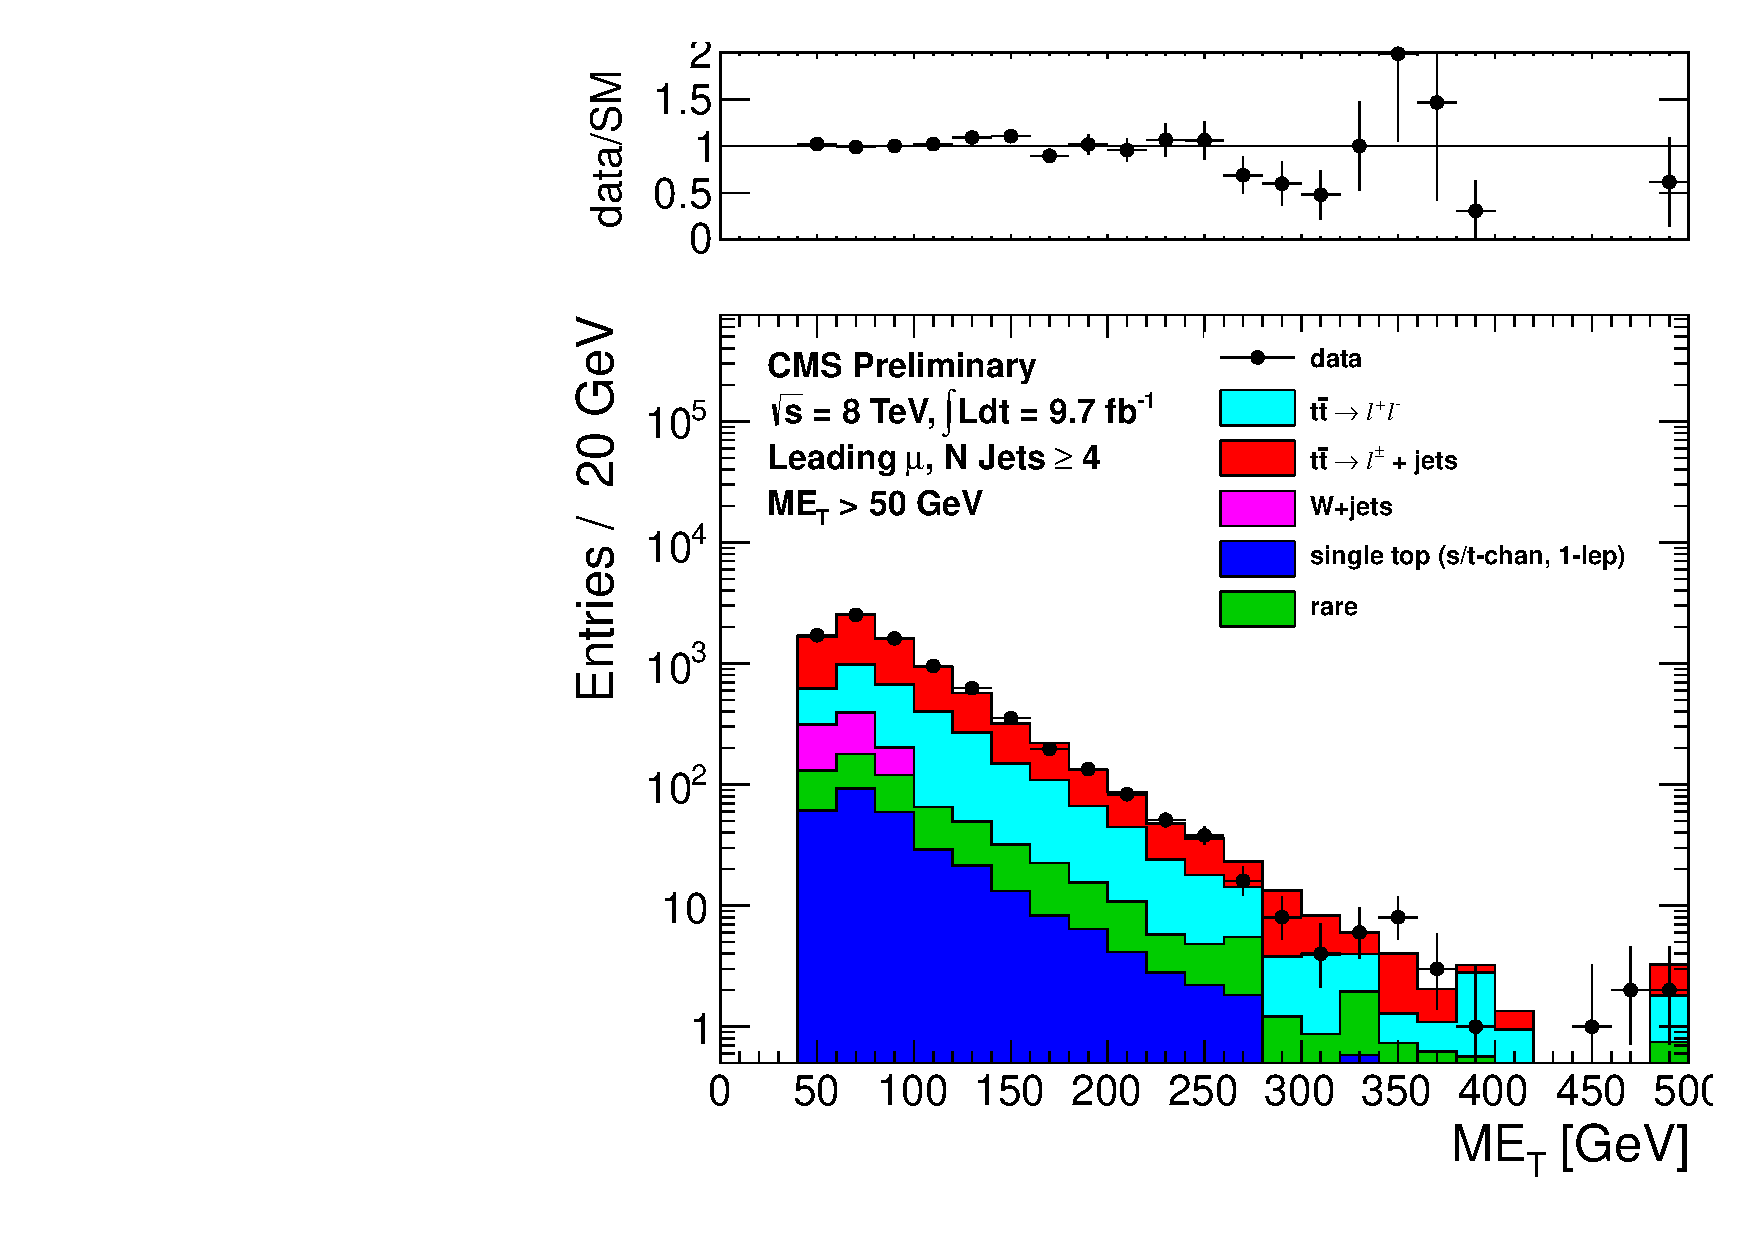
\includegraphics[width=0.5\linewidth]{plots/CR5plots/met_met50_leadmuo_nj4.pdf}%
        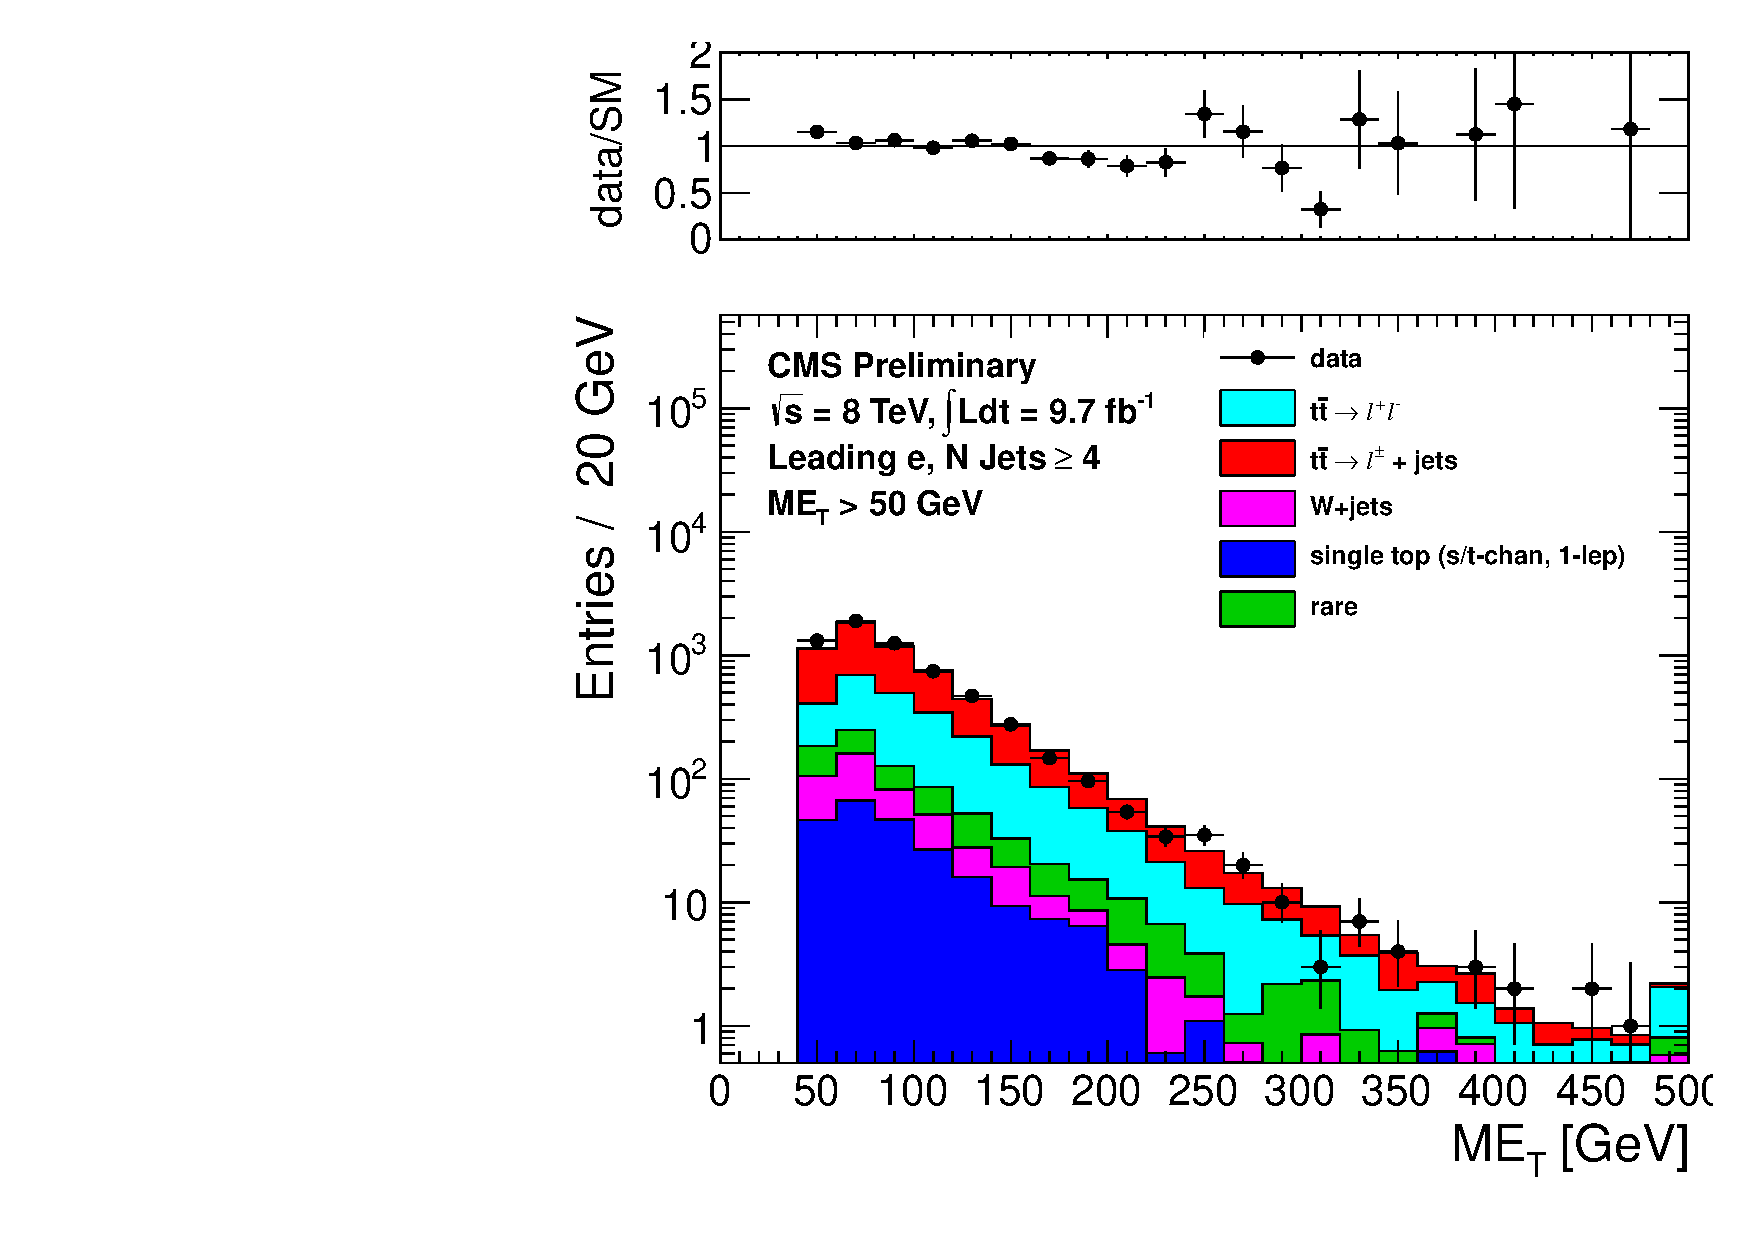
\includegraphics[width=0.5\linewidth]{plots/CR5plots/met_met50_leadele_nj4.pdf}
        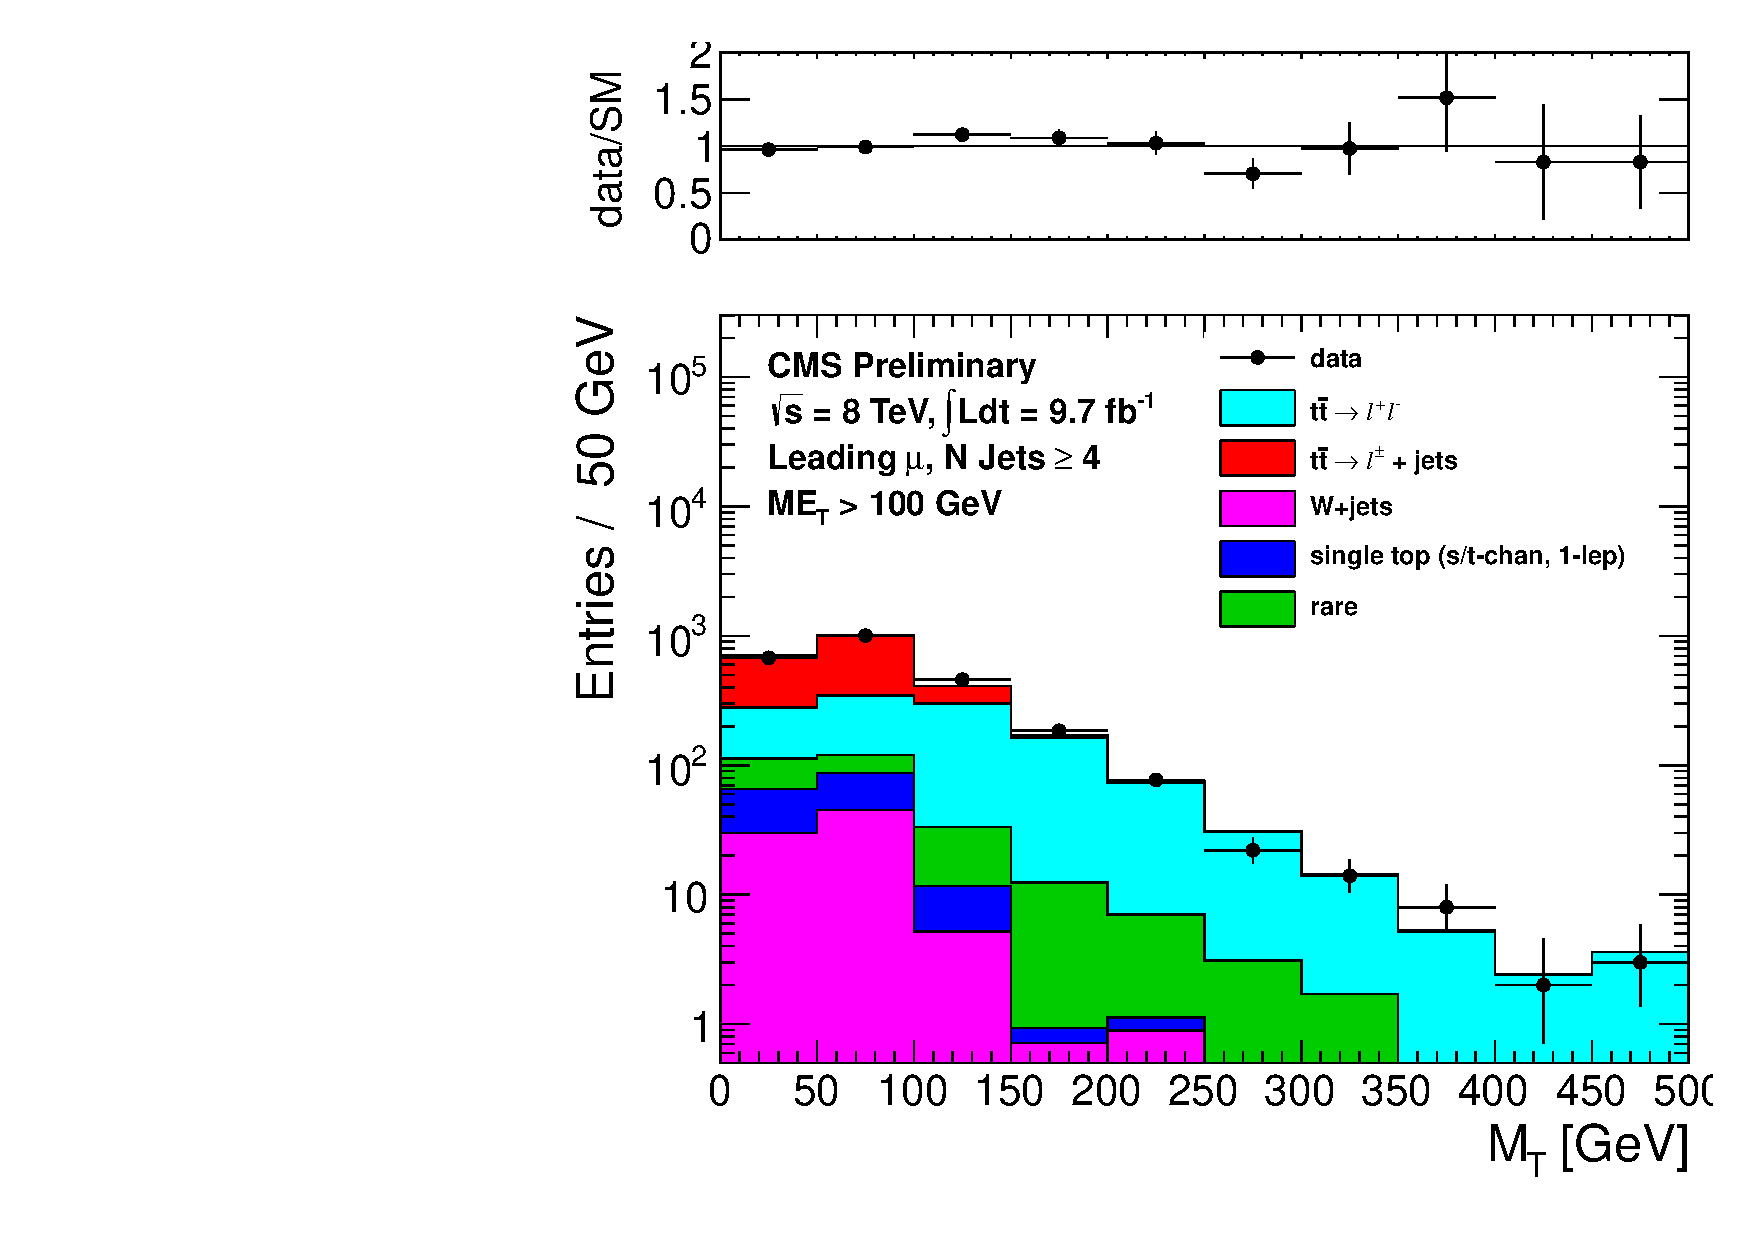
\includegraphics[width=0.5\linewidth]{plots/CR5plots/mt_met100_leadmuo_nj4.pdf}%
        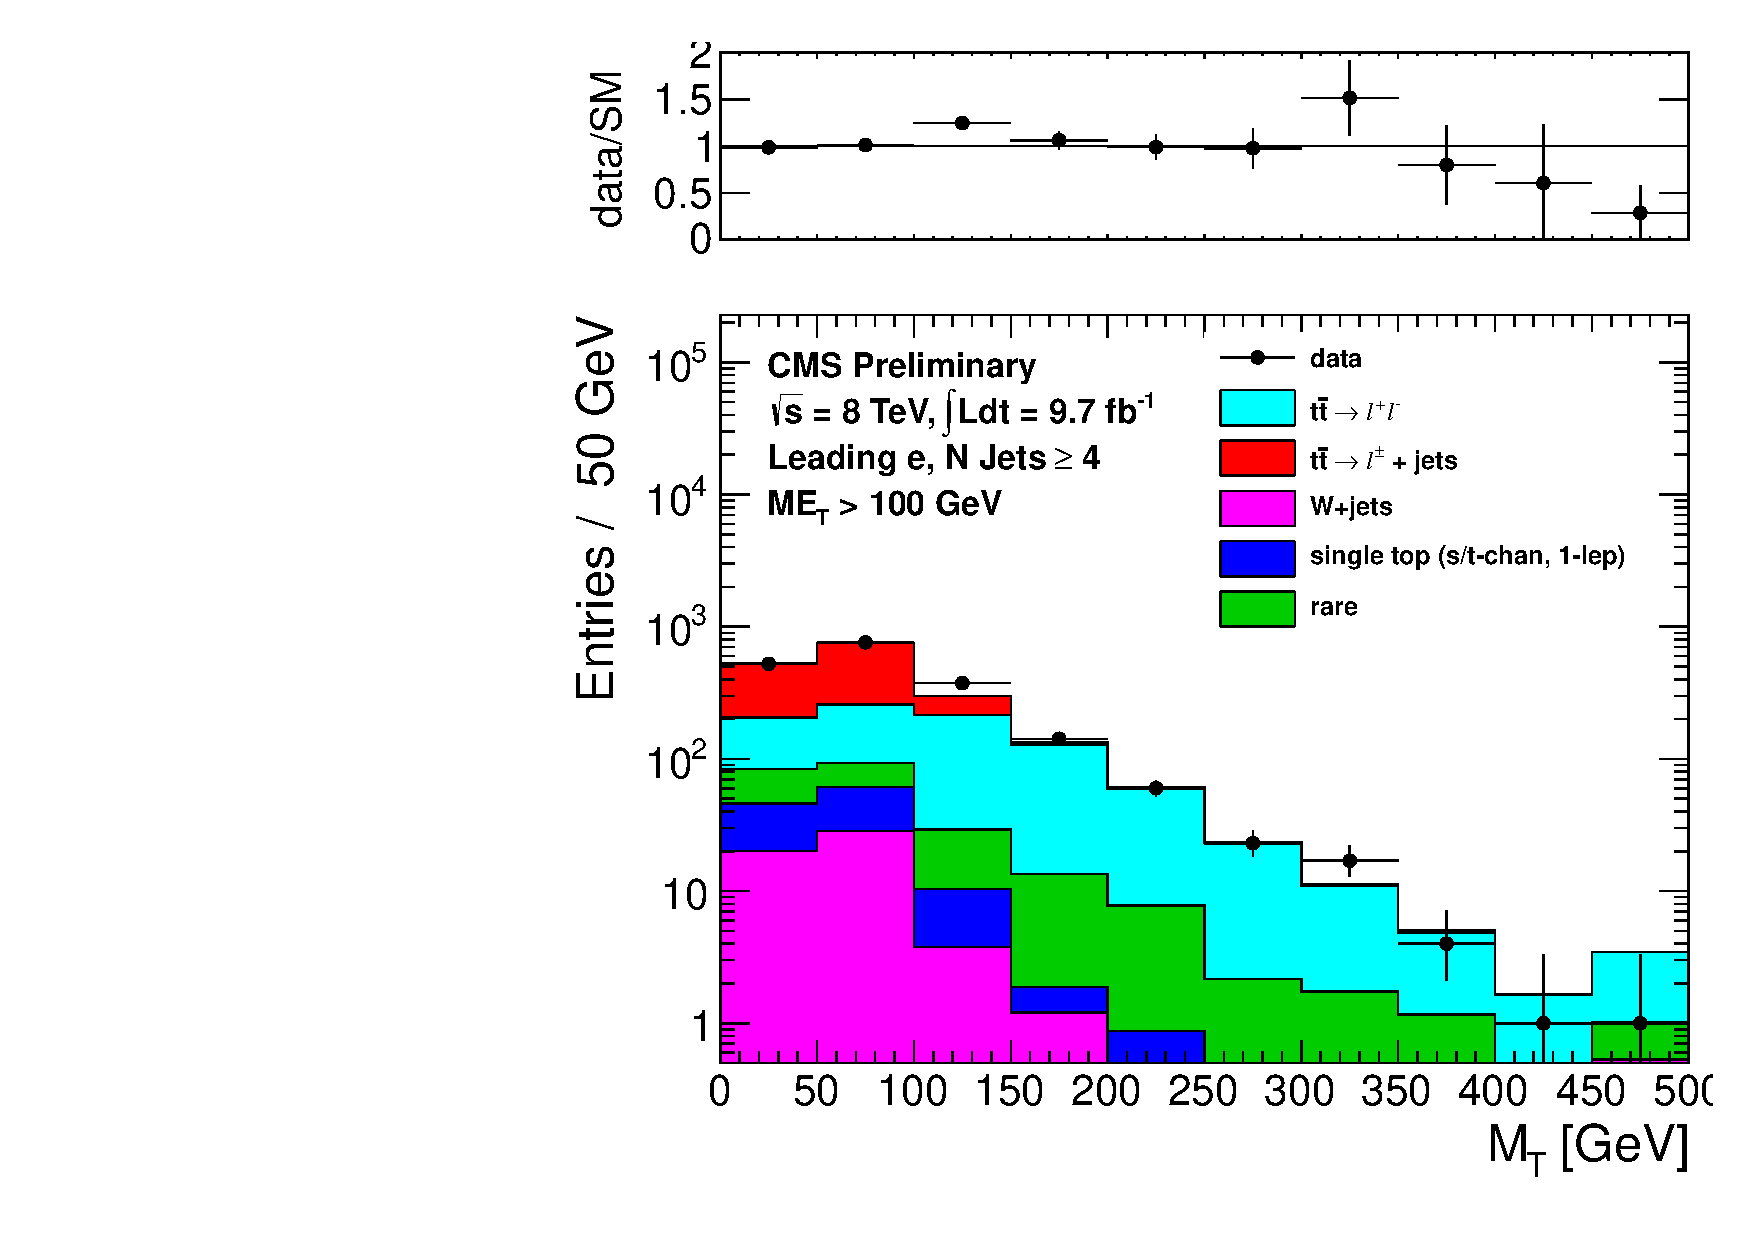
\includegraphics[width=0.5\linewidth]{plots/CR5plots/mt_met100_leadele_nj4.pdf}
    \caption{
      Comparison of the \met\ (top) and \mt\ for $\met>100$ (bottom) distributions in data vs. MC for events
      with a leading muon (left) and leading electron (right)
      satisfying the requirements of CR5. 
\label{fig:cr5met} 
}  
      \end{center}
\end{figure}

\begin{figure}[hbt]
  \begin{center}
        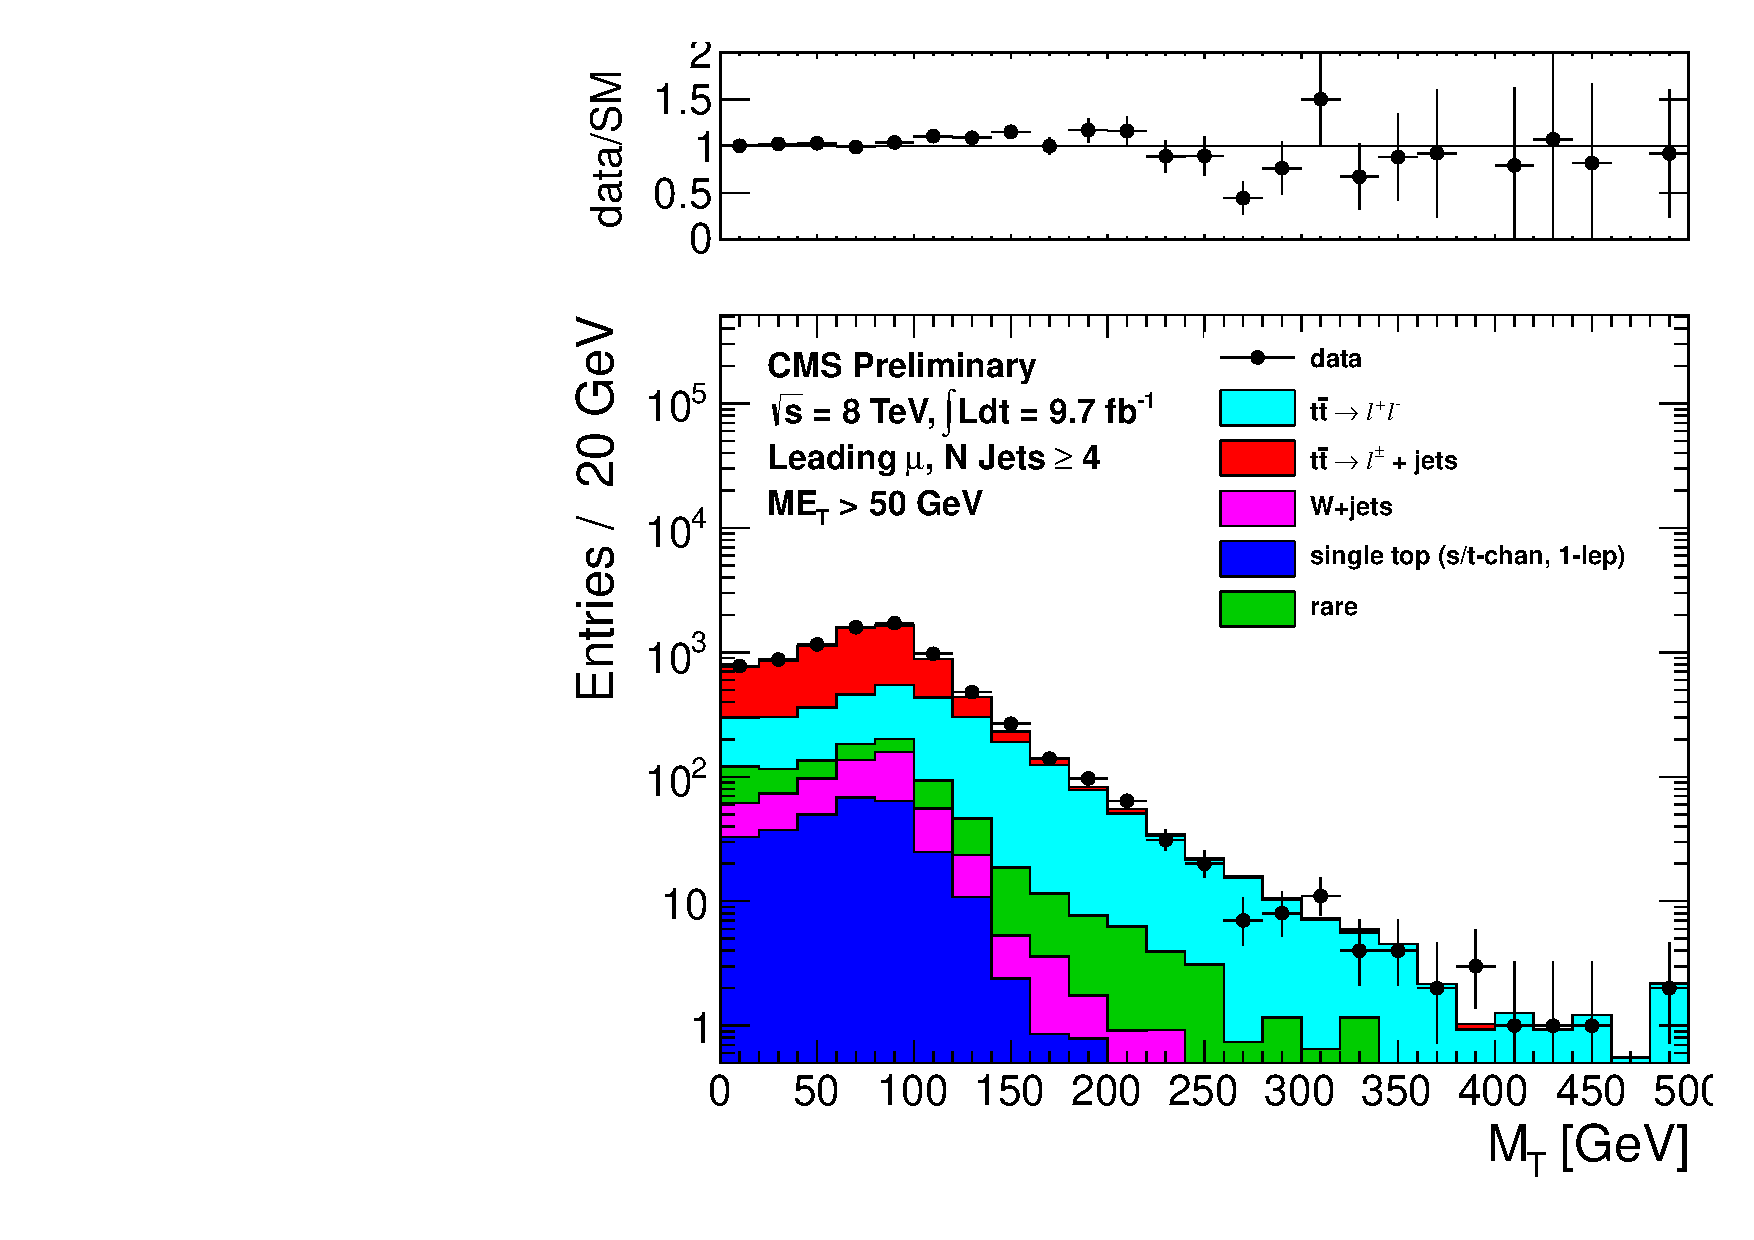
\includegraphics[width=0.5\linewidth]{plots/CR5plots/mt_met50_leadmuo_nj4.pdf}%
        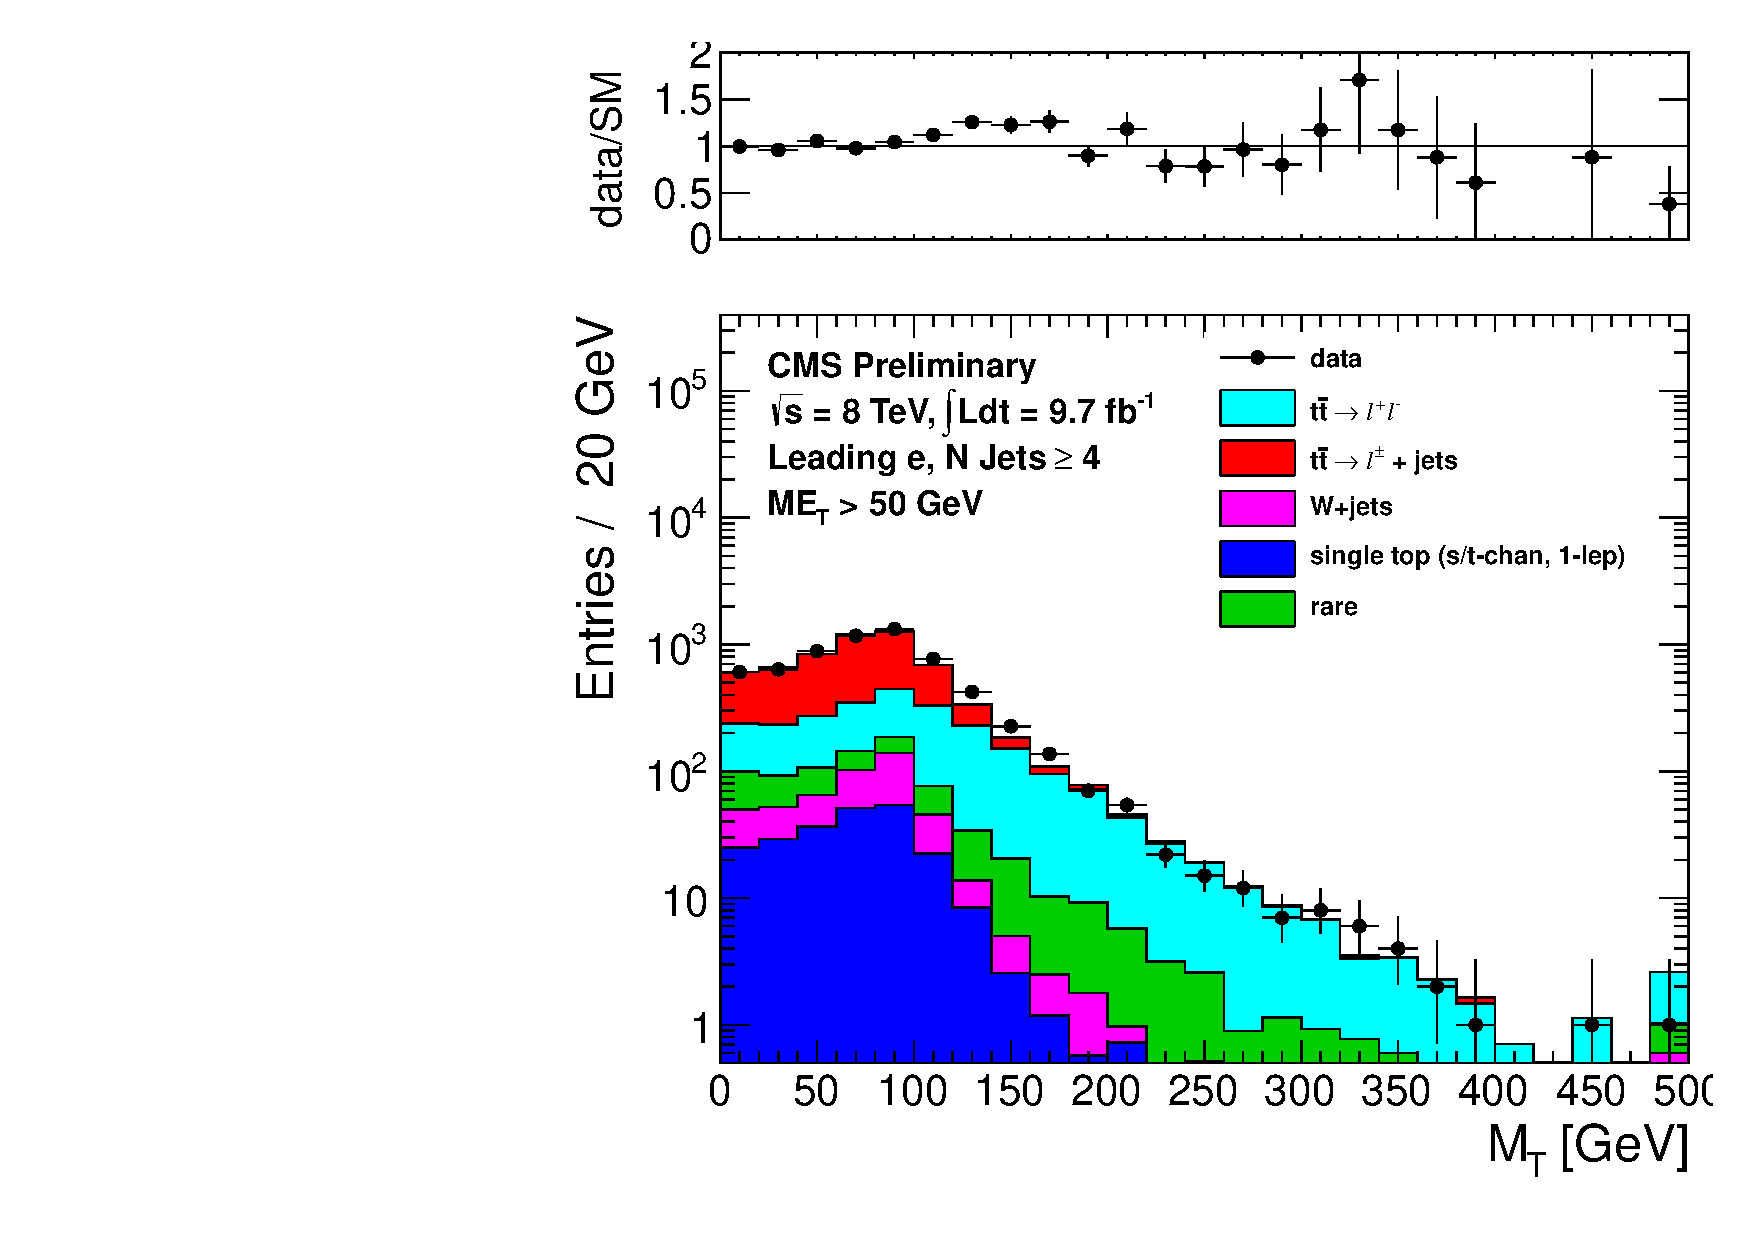
\includegraphics[width=0.5\linewidth]{plots/CR5plots/mt_met50_leadele_nj4.pdf}
        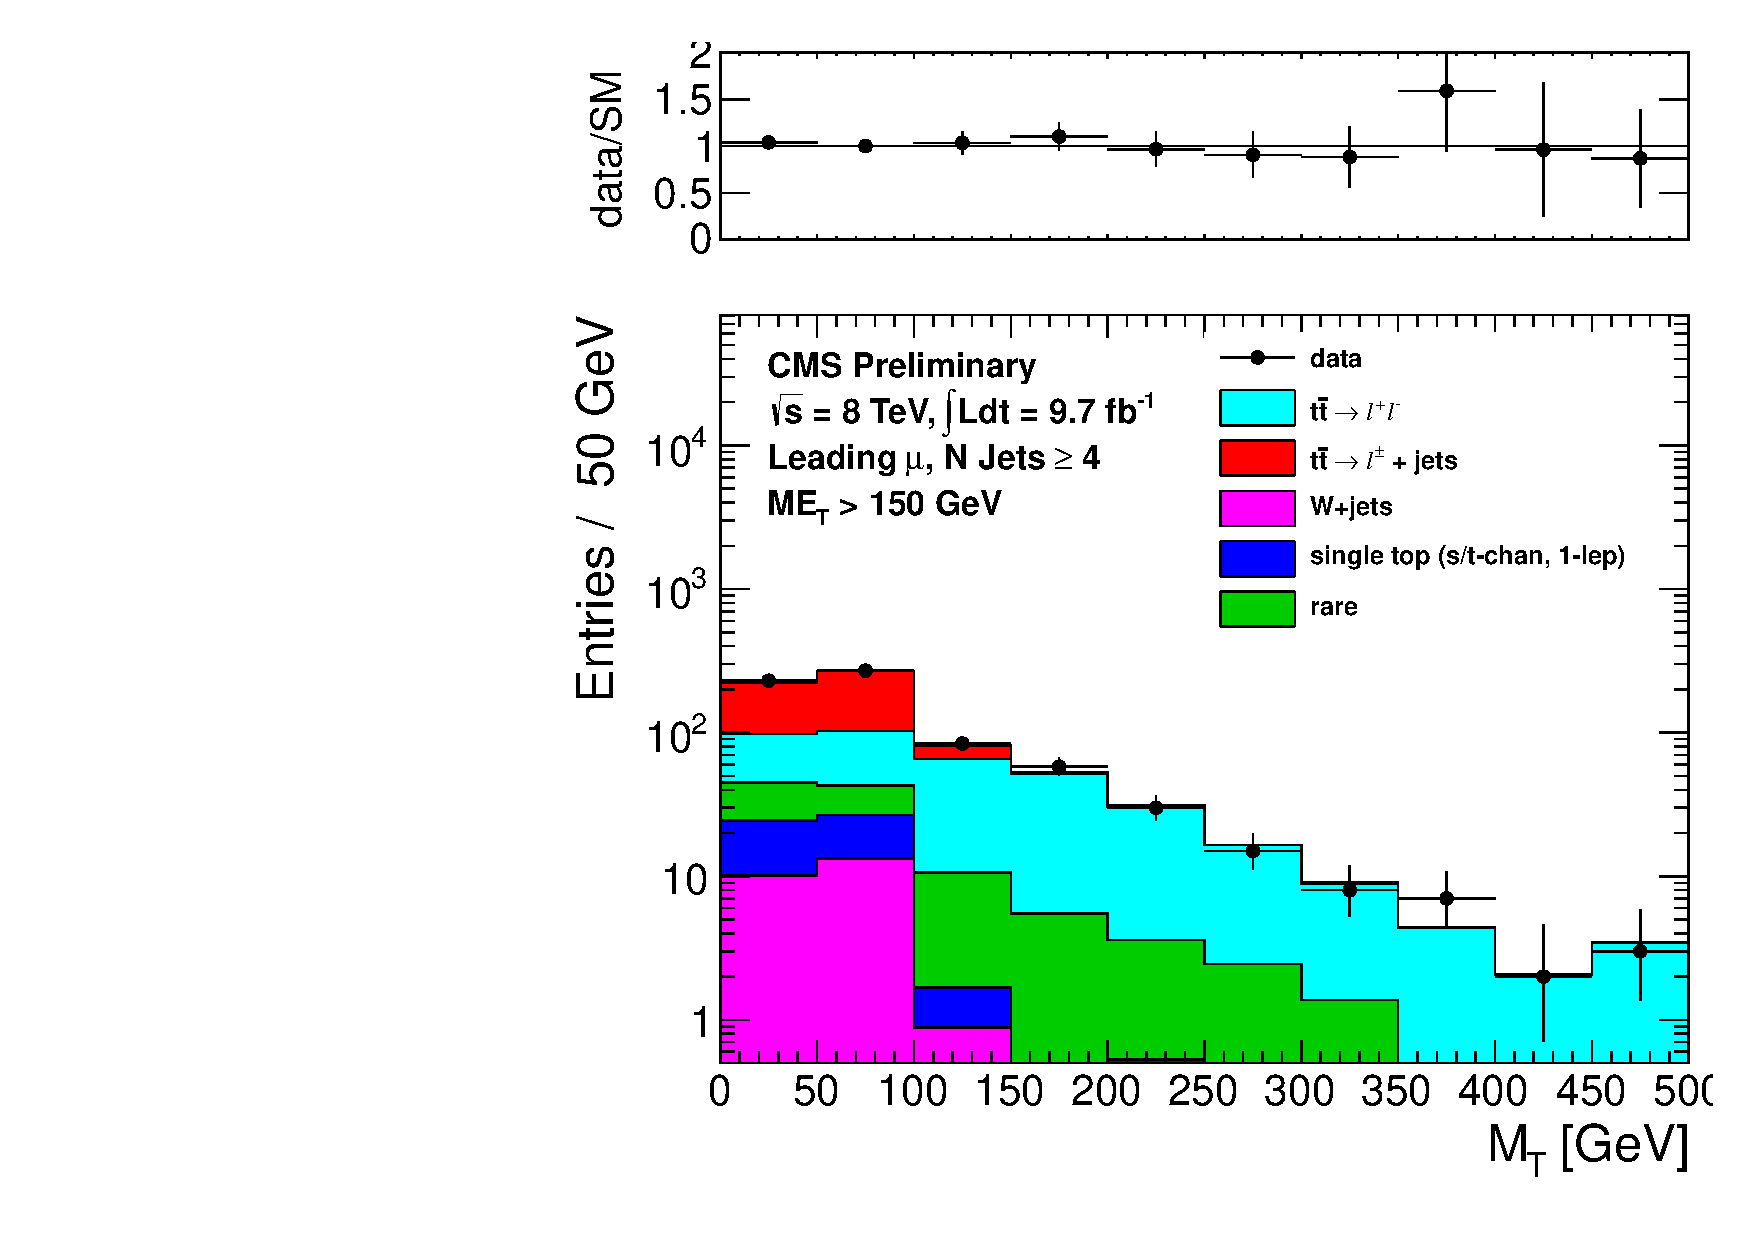
\includegraphics[width=0.5\linewidth]{plots/CR5plots/mt_met150_leadmuo_nj4.pdf}%
        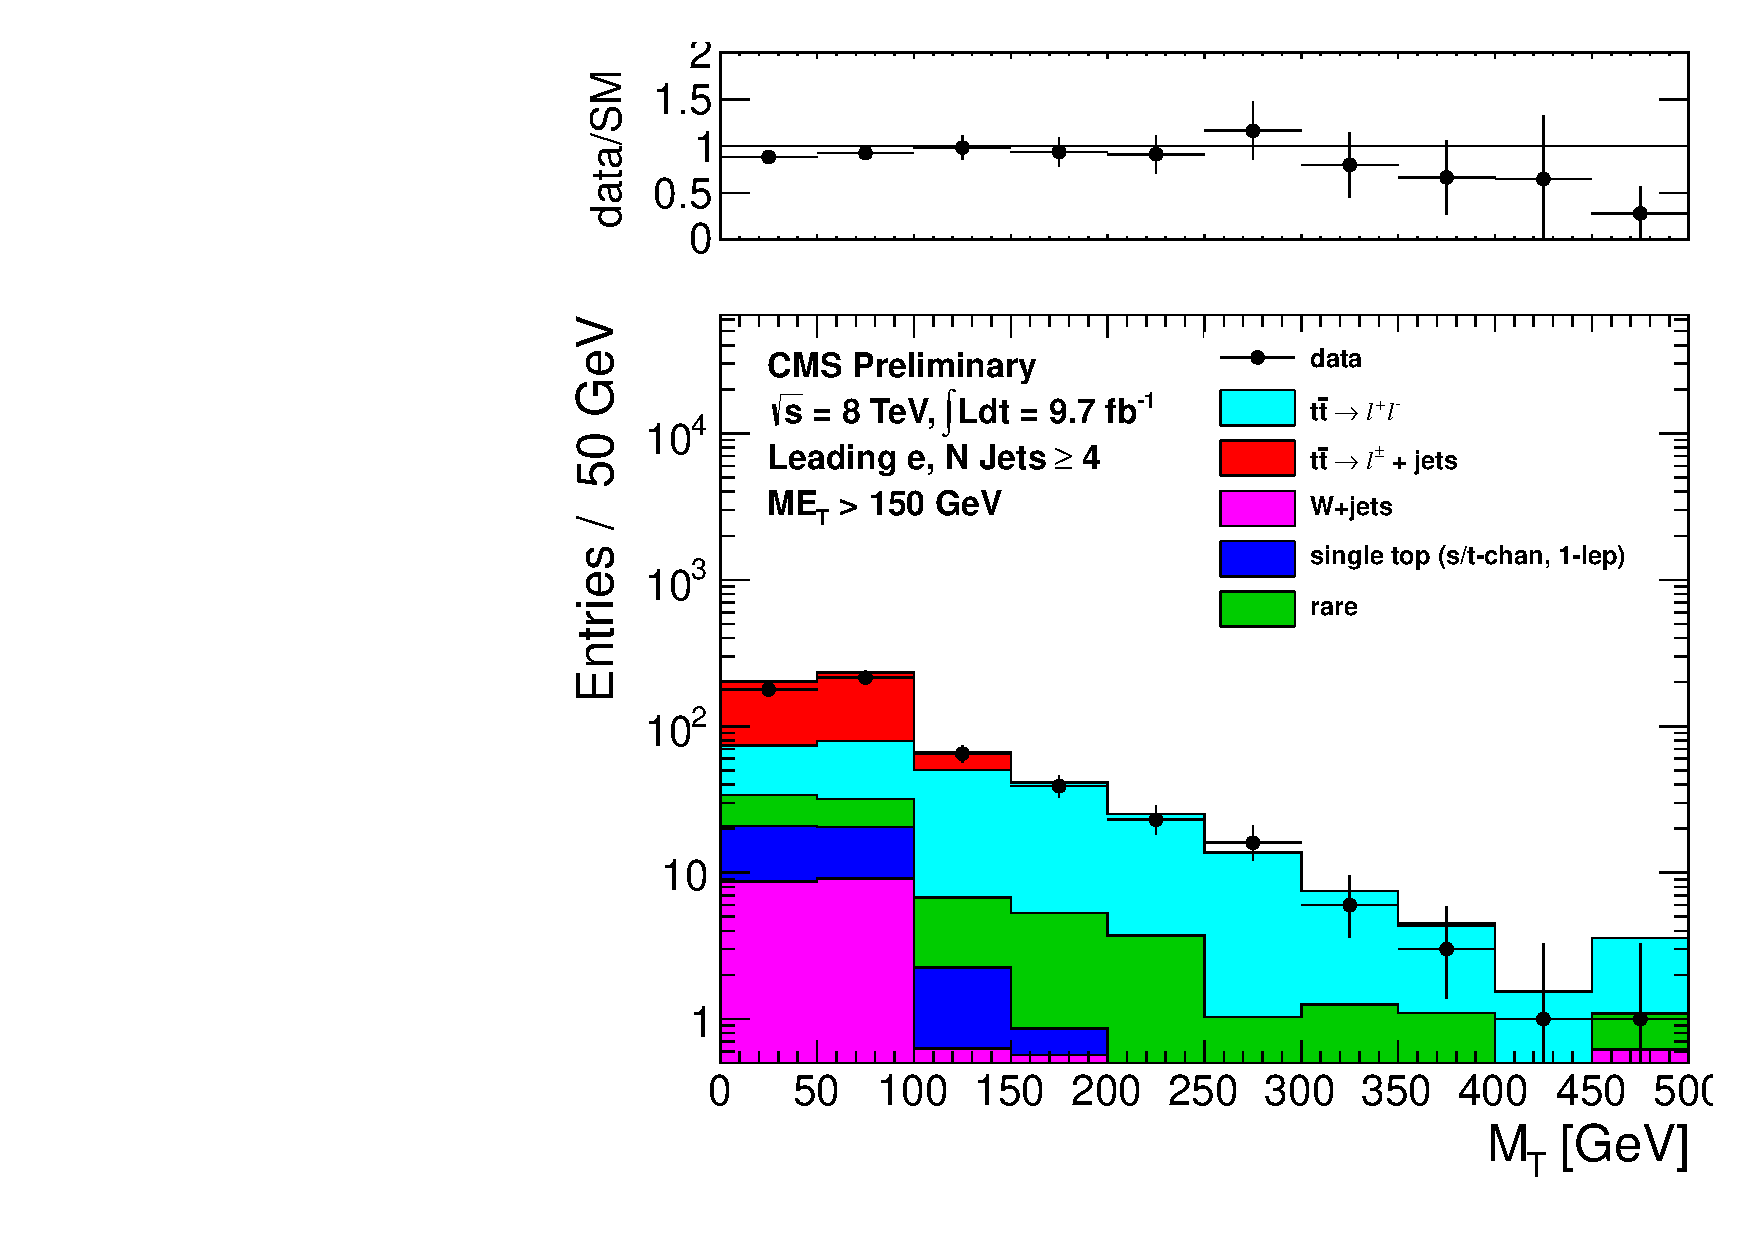
\includegraphics[width=0.5\linewidth]{plots/CR5plots/mt_met150_leadele_nj4.pdf}
        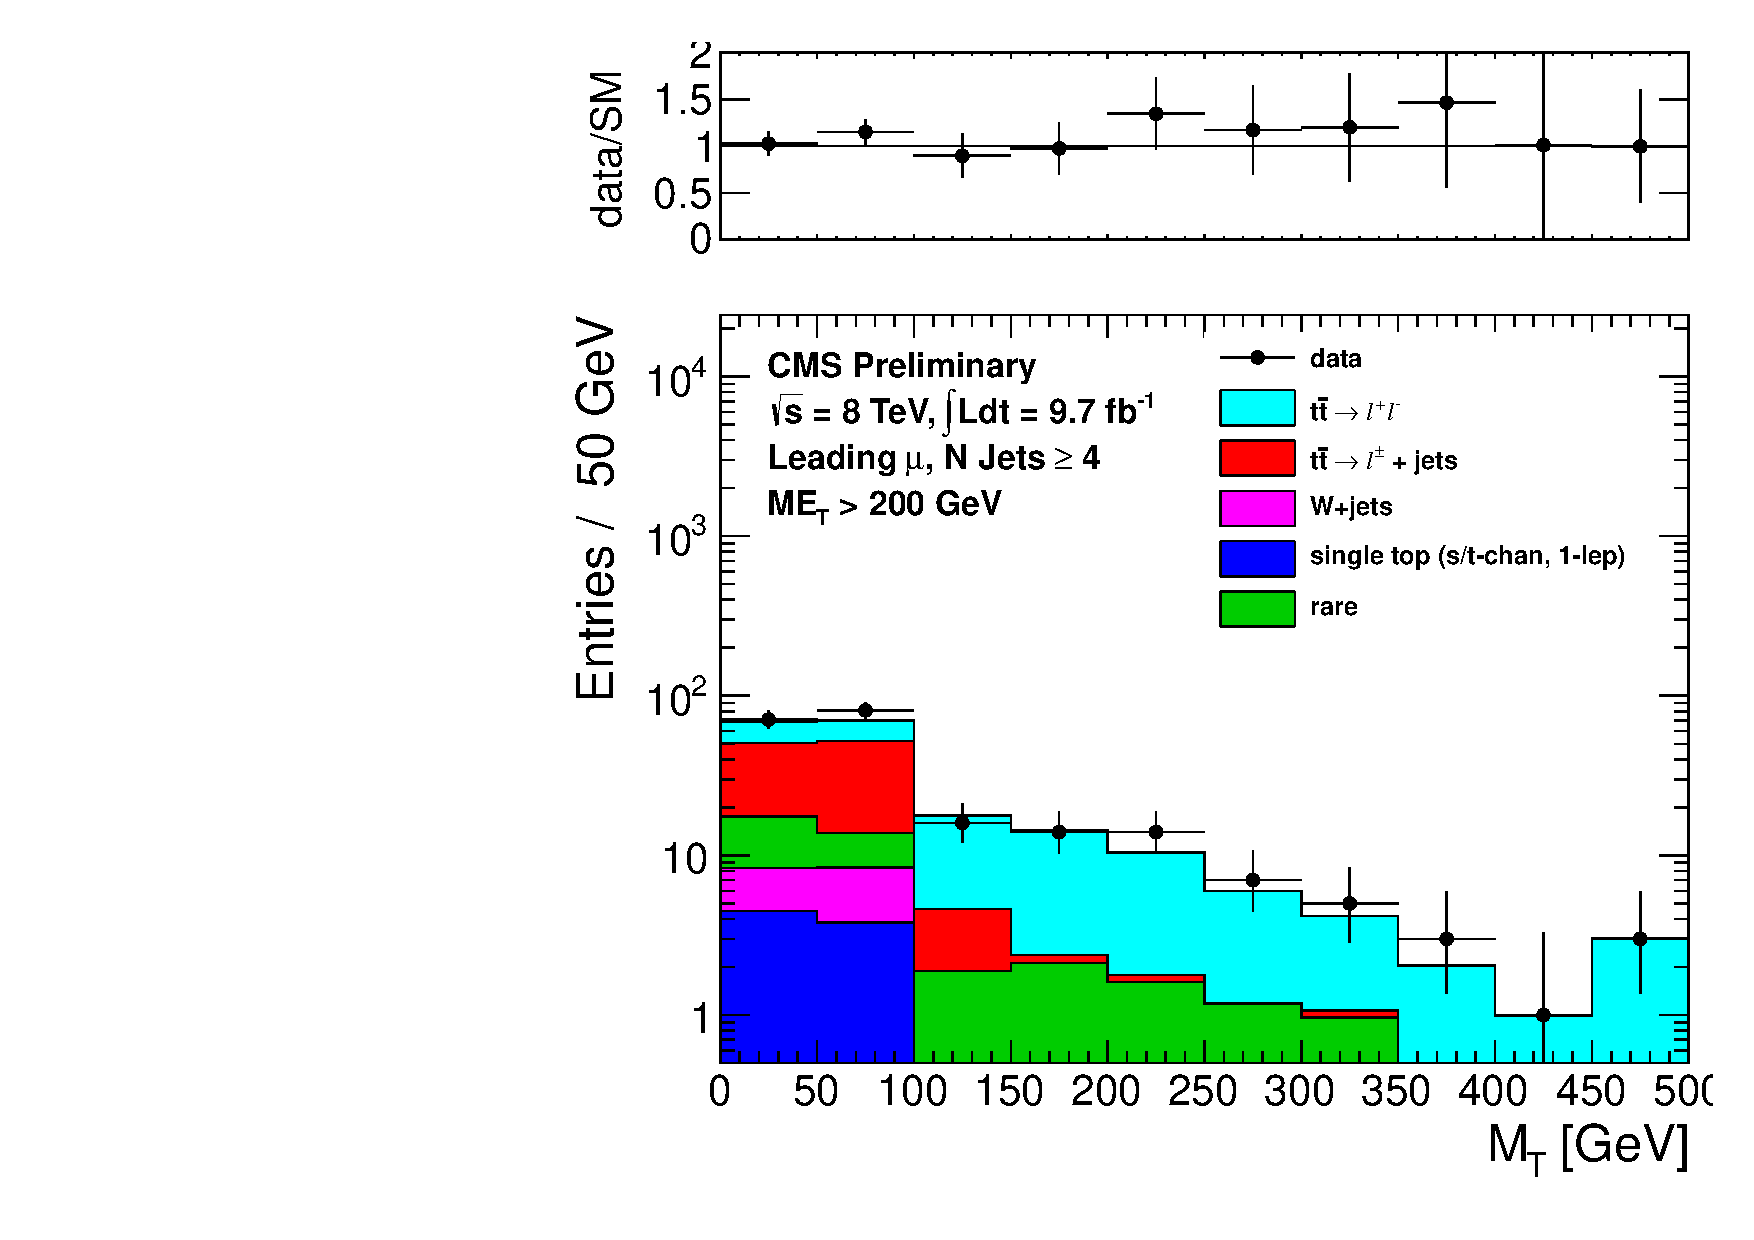
\includegraphics[width=0.5\linewidth]{plots/CR5plots/mt_met200_leadmuo_nj4.pdf}%
        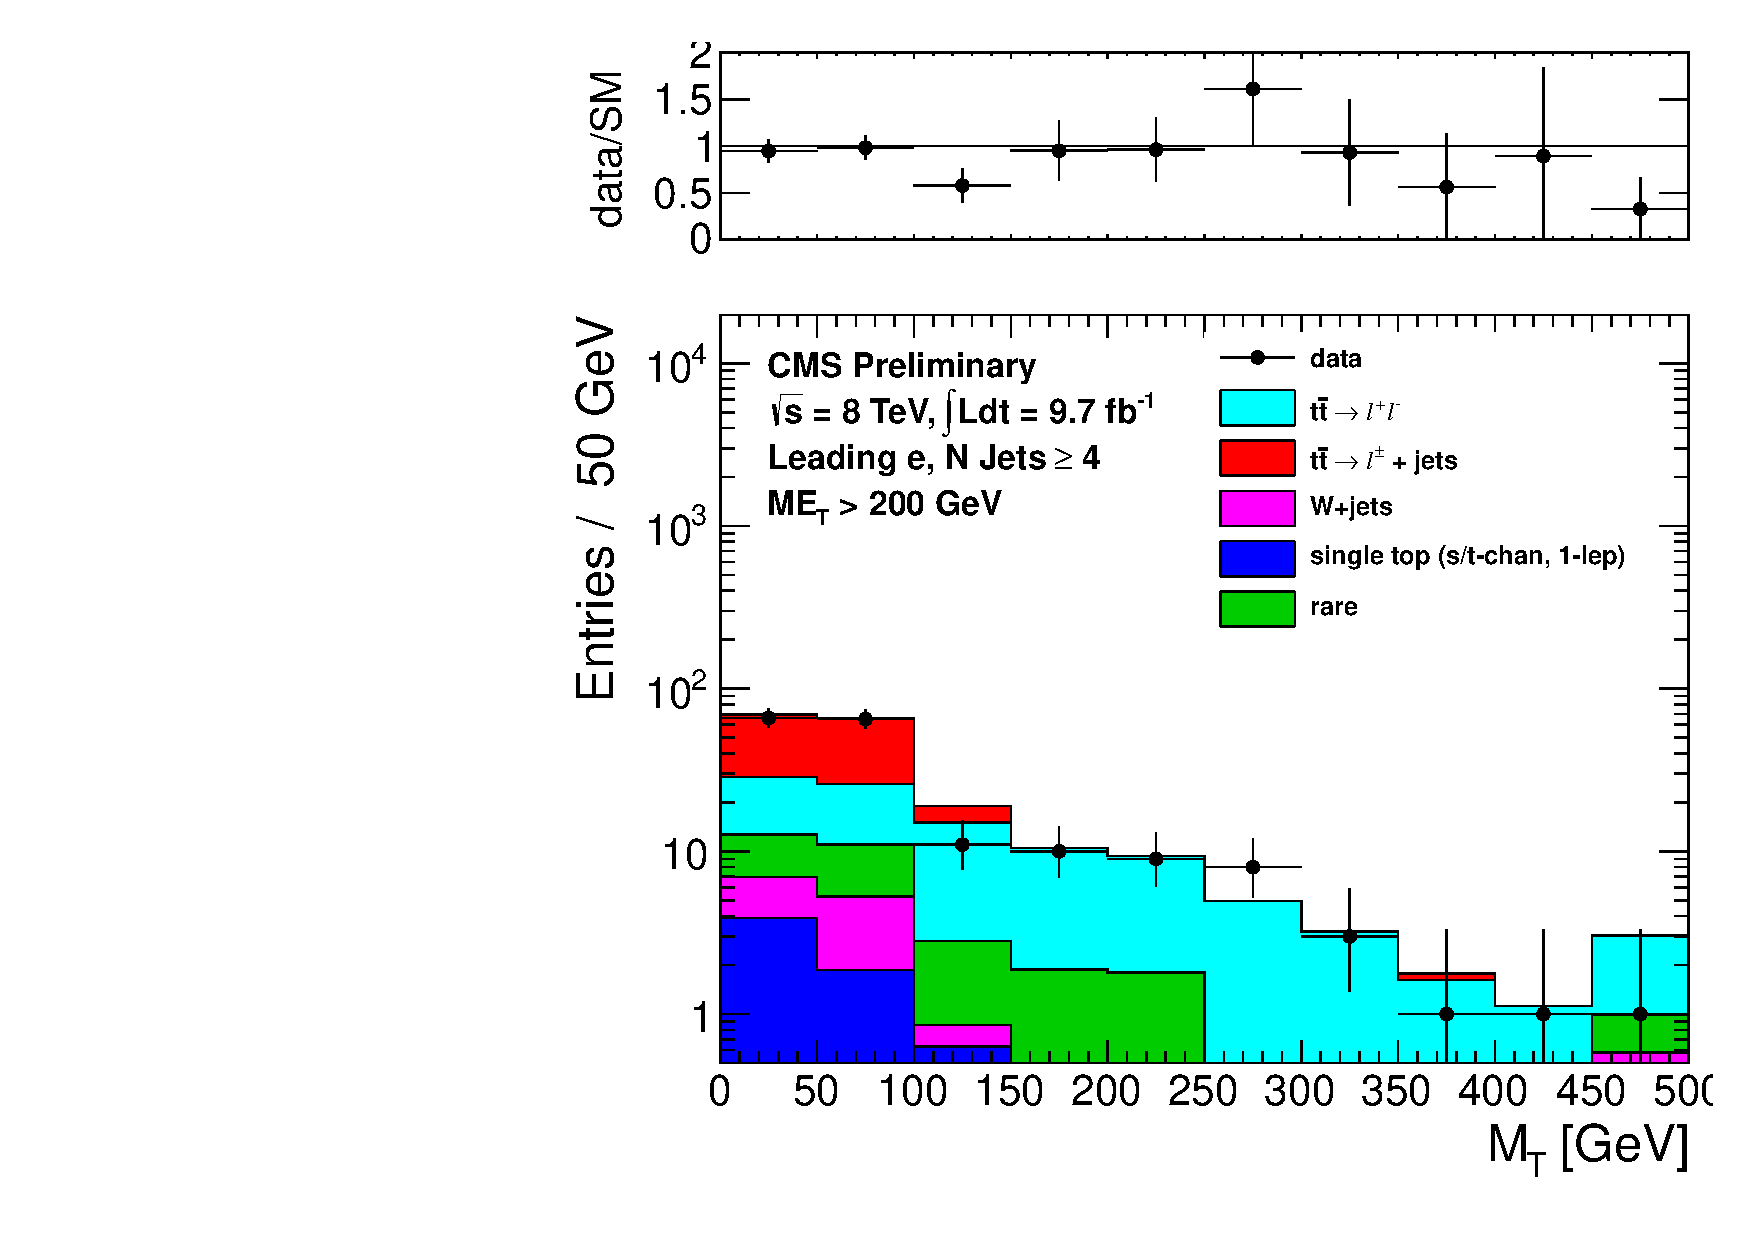
\includegraphics[width=0.5\linewidth]{plots/CR5plots/mt_met200_leadele_nj4.pdf}
%        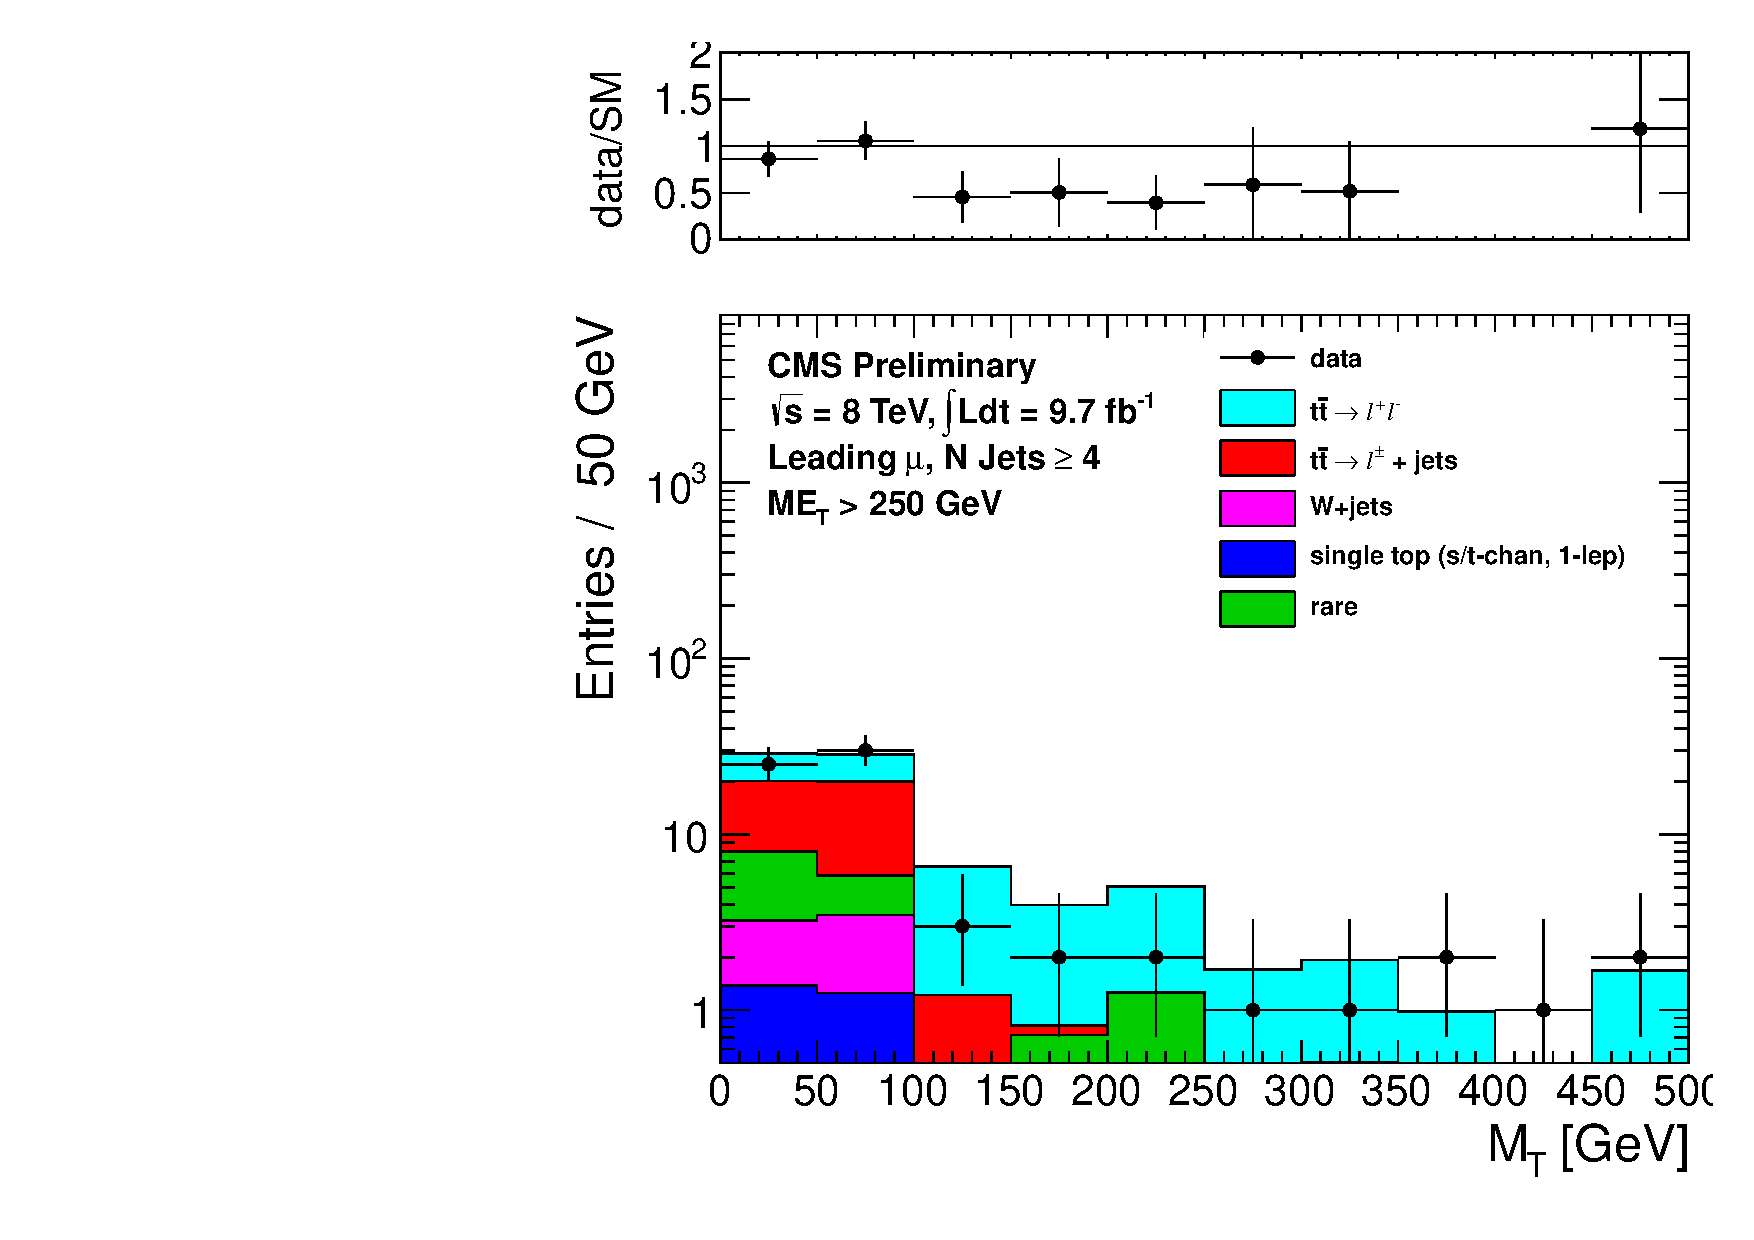
\includegraphics[width=0.5\linewidth]{plots/CR5plots/mt_met250_leadmuo_nj4.pdf}%
%        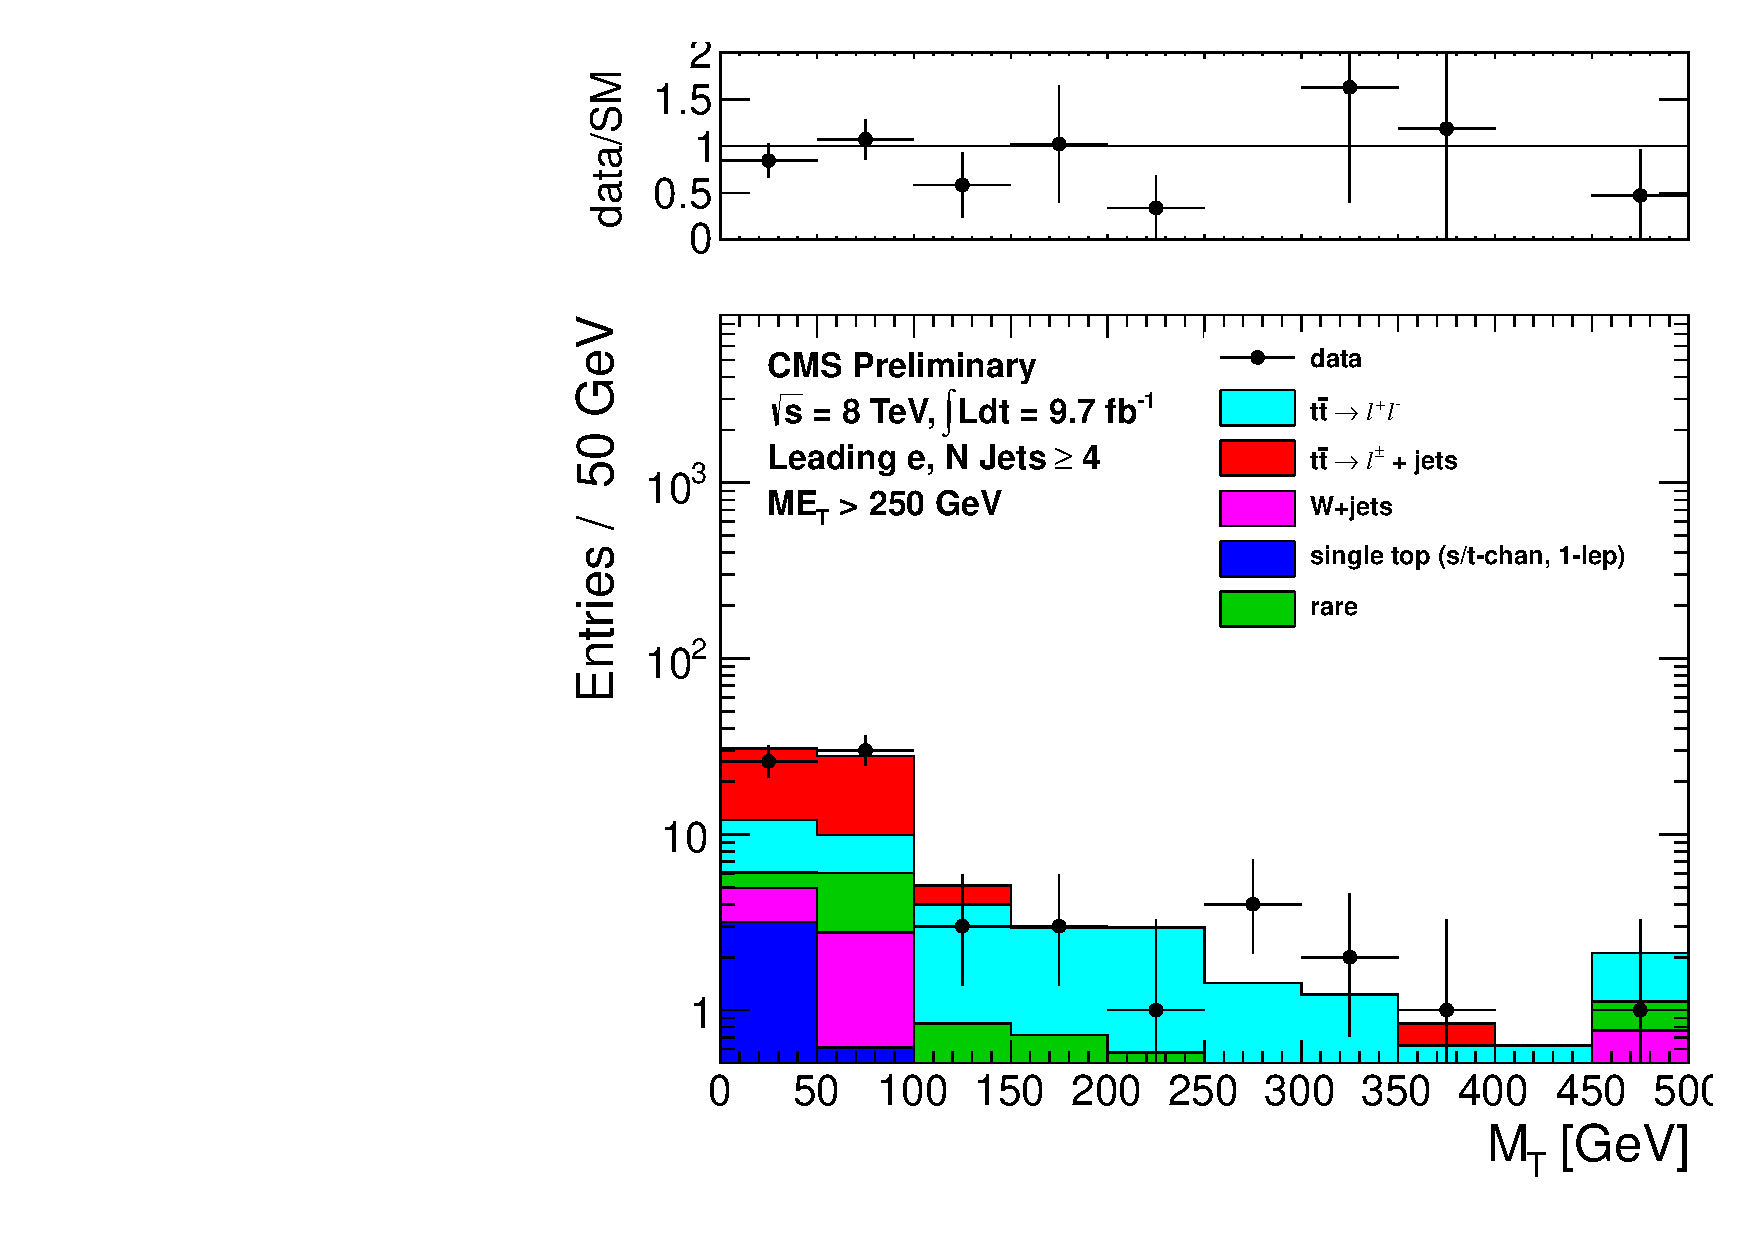
\includegraphics[width=0.5\linewidth]{plots/CR5plots/mt_met250_leadele_nj4.pdf}
    \caption{
      Comparison of the \mt\ distribution in data vs. MC for events
      with a leading muon (left) and leading electron (right)
      satisfying the requirements of CR5. The \met\ requirements used are
      50 GeV (top), 150 GeV (middle) and 200 GeV (bottom).
\label{fig:cr5mtrest} 
}  
      \end{center}
\end{figure}


\begin{figure}[hbt]
  \begin{center}
        \includegraphics[width=0.5\linewidth]{plots/CR5plots/mt_met250_leadmuo_nj4.pdf}%
        \includegraphics[width=0.5\linewidth]{plots/CR5plots/mt_met250_leadele_nj4.pdf}
        \includegraphics[width=0.5\linewidth]{plots/CR5plots/mt_met300_leadmuo_nj4.pdf}%
        \includegraphics[width=0.5\linewidth]{plots/CR5plots/mt_met300_leadele_nj4.pdf}
        \includegraphics[width=0.5\linewidth]{plots/CR5plots/mt_met350_leadmuo_nj4.pdf}%
        \includegraphics[width=0.5\linewidth]{plots/CR5plots/mt_met350_leadele_nj4.pdf}
%        \includegraphics[width=0.5\linewidth]{plots/CR5plots/mt_met250_leadmuo_nj4.pdf}%
%        \includegraphics[width=0.5\linewidth]{plots/CR5plots/mt_met250_leadele_nj4.pdf}
    \caption{
      Comparison of the \mt\ distribution in data vs. MC for events
      with a leading muon (left) and leading electron (right)
      satisfying the requirements of CR5. The \met\ requirements used are
      250 GeV (top), 300 GeV (middle) and 350 GeV (bottom).
\label{fig:cr5mtrest2} 
}  
      \end{center}
\end{figure}


\clearpage



%\section{Background Estimation}
%   \label{sec:backgrounds}
%  
In order to search for a possible signal from stop decays giving rise to a signature of \ttbar\ with additional \met\
from the LSPs, it is necessary to determine the composition of the SM backgrounds in the signal region. 
This section details the methods pursued to estimate the background in the signal sample and describes the 
procedure to estimate the systematic uncertainties. The general strategy is to use the MC prediction for the 
backgrounds after applying corrections derived from data. 

The most important background to a stop signal arises from SM \ttbar. The \ttbar\ background may be 
separated into contributions containing a single lepton \ttlj\ and two leptons \ttll. As described in this section, 
the \ttll\ background is the dominant process in our signal region (\met\ $>$ 100~\GeV and \mt\ $>$ 150~\GeV, $\ge 1$ b-tags, isolated track veto),
contributing $\sim 80\%$ of the background yield.
%
This background has large true \met\ and consequently larger \mt\ due to the presence of two neutrinos.
Additional contributions to the single lepton sample arise from \wjets\ and single top. The combination of 
all single lepton backgrounds, \ttlj, \wjets\ and single top, comprises $\sim 15\%$ of the signal sample. 
Finally, other background sources such as dibosons, \dy\ + jets, in addition to rarer processes such as \ttbar\ 
produced in association with a vector boson and tribosons, provide a combined contribution to the signal sample 
at the level of $\sim 5\%$.
Finally, the QCD background contribution is small, particularly in the signal sample, with a large \met\ requirement.

The total bkg in the signal region is estimated according to:

$$ N_{bkg}  = N_{1 lep} + N_{2 lep} + N_{rare} $$

$$ N_{1 lep} = N_{1 lep}^{MC} 
\times 
{(1- \epsilon_{fake})^{data} \over (1 - \epsilon_{fake})^{MC}} 
\times 
{N_{peak}^{data} \over N_{peak}^{MC}}
$$

$$ N_{2 lep} = N_{2 lep}^{MC} 
\times 
{(1- \epsilon_{iso\ trk})^{data} \over (1 - \epsilon_{iso\ trk})^{MC}} 
\times 
{N_{peak}^{data} \over N_{peak}^{MC}}
$$

All of these terms will be defined clearly in this section, including their corrections and sources of systematic errors.

 % \label{sec:bkg_intro}

\clearpage 

%  \subsection{Single Lepton Backgrounds}
%   \label{sec:bkg_singlelep}
%  
This category of backgrounds includes processes with a single leptonic \W~decay, giving rise to one lepton and \met\ from a single neutrino.
As a result, the \mt\ variable, constructed from the lepton and the \met, exhibits a kinematic edge at $\mt \sim \mW$. The main contributors
to this background are \ttlj, \wjets\ and single top, though in the latter case there is a contribution from \tw\ that can give rise to two leptons. 
As shown in Figure.~\ref{fig:mtsinglelepcomp} (left), these backgrounds exhibit a similar \mt\ shape and are thus combined into a single 
background estimate. 

It should be underlined that single lepton events entering the signal sample are in the far \mt~tail for these processes
and contribute mainly due to the \met\ resolution that smears the \mt\ peak, particularly in the presence of multiple jets. 
Since these types of effects are challenging to model in simulation, the background estimate for this category of processes is cross checked 
in a control sample in data. 
%
%The control sample is obtained by applying the full selection criteria with the exception of the b-tagging requirement, 
%that is reversed, vetoing events with b-tagged jets. 
%
The control sample used here is the b-veto region defined in Section~\ref{sec:selection}. \met $> 100$~\GeV is required and the 
isolated track veto is not applied.
%
The b-tag veto greatly reduces the contamination from \ttbar, which is particularly important
in the case of \ttll\ which otherwise populates the \mt\ tail. The resulting sample is dominated by \wjets\ events. The derivation of the background 
estimate in this control sample serves to validate the method. 
In addition, the level of agreement between the prediction and the data in the \mt\ tail provides an estimate of the systematic uncertainty for this
background prediction. 

\begin{figure}[hbt]
  \begin{center}
	\includegraphics[width=0.5\linewidth]{plots/mt_singlelepcomp_full.png}%
        \includegraphics[width=0.5\linewidth]{plots/mt_bkgsubt_bveto_met50.png}
	\caption{
	  \label{fig:mtsinglelepcomp}%\protect 
          Monte Carlo comparison of the shapes (left) of the \mt\ distribution for the main background processes containing a single leptonic \W\ decay (left).
          The \mt\ shape for \ttlj, \wjets\ and single top are similar and thus combined into a single background estimate. Comparison of the MC 
        prediction (right) for single lepton processes (blue) and the data after subtracting the non-single lepton background MC prediction.
        The latter is overlayed in red to show the scale of the subtraction. 
        Since the control sample is dominated by $\Wfourj$ events, 
        the MC is not expected to provide an estimate of the overall normalization to better than the $\sim 15\%$ difference observed.}
  \end{center}
\end{figure}

To validate the single lepton bkg estimate, we take the right plot in Figure~ref{fig:mtsinglelepcomp},
form the ratio of yields in the peak region in data (after non-single lepton subtraction), $N_{peak}^{data}$, and in lepton plus jets MC, $N_{peak}^{MC}$, 
and multiply this ratio by the yield in the tail in lepton plus jets MC, $N_{tail}^{MC}$. The non-single lepton subtraction applied to data is obtained from MC.
We do so for two \met requirements as shown in Table~\ref{tab:ljetsclosure}. 
%Based on the statistical precision of this closure test, we assign a 30\%
%systematic error to the single lepton bkg estimation technique.

%The single lepton background contribution to the tail of the \mt\ is derived from MC and normalized to the data in the \mt\ peak region, defined by the 
%range $60 < \mt \le 100~\GeV$. In particular, the total yield for the combination of the single lepton + jets samples in MC satisfying $60 < \mt \le 100~\GeV$
%is scaled to match the entries in data satisfying the same \mt\ requirement. The data is corrected for the expected contamination from non-single 
%lepton + jets processes, which is obtained from MC. The derivation of this MC to data scale factor is shown in Figure.~\ref{fig:mtsinglelepcomp} (right), where the 
%contribution from non-single lepton + jets processes in the \mt\ peak is also shown to be small. 
%Scaling to the data yield in the \mt\ peak largely reduces the dependence on the \ttbar\ cross section and cancels systematic uncertainties associated with
%effects such as the luminosity, selection efficiencies, etc$\dots$
 

\begin{figure}[!ht]
  \begin{center}
	\includegraphics[width=0.5\linewidth]{plots/mt_met50_bveto.pdf}%
        \includegraphics[width=0.5\linewidth]{plots/mt_met100_bveto.pdf}
	\caption{
	  \label{fig:mtbveto}%\protect 
          Comparison of data and MC in the b-veto sample after scaling the single lepton samples in the \mt\ peak region ($60-100~\GeV$) for two \met\ requirements
          $\met>50~\GeV$ (left) and $\met>100~\GeV$ (right). The simulation shows reasonable agreement with the data both in the peak and the \mt\ tail, as can also 
          be seen the ratios.}  
      \end{center}
\end{figure}


\begin{figure}[!hb]
  \begin{center}
        \includegraphics[width=0.5\linewidth]{plots/mt_singlelepcomp_full_stack.png}%
	\includegraphics[width=0.5\linewidth]{plots/bkg_comp_err_mt_met100.png}
	\caption{
	  \label{fig:mtsamplecomperr}%\protect 
          Stacked plot (left) showing the relative sample composition in MC for the main single lepton + jets components, \ttlj, \wjets\ and single top
          sample for the b-veto control selection. Note no scalings are applied and the $\met>50~\GeV$ is shown. Percent change in the total single lepton + jets
          background prediction for variations in the normalization of each single lepton + jets background component (right). Each sample is varied independently and the
          full background prediction is performed.}
      \end{center}
\end{figure}


\begin{table}[!ht]
\begin{center}
\begin{tabular}{c|c|c}
\hline
Sample                   &   $\met>50~\GeV$  &   $\met>100~\GeV$  \\
                         &   $M_T > 150~\GeV$& $M_T > 150~\GeV$ \\
\hline
\hline
Lepton + Jets Prediction           & $88 \pm 12$  & $38 \pm 8$   \\
Data in Signal Region               & $106 \pm 13$ & $40 \pm 8$   \\
\hline
Data/MC Closure                     & $1.20 \pm 0.22$ & $1.03 \pm 0.30$   \\
\hline
\end{tabular}
\caption{Summary of closure test in b-veto control sample for two values of the \met\ requirement. The closure serves to estimate the systematic uncertainty for 
  the prediction of the single lepton + jets background.\label{tab:ljetsclosure}}
\end{center}
\end{table}

Figure~\ref{fig:mtbveto} shows a comparison of the \mt\ distribution in data and MC in the b-veto control sample for two values of the \met\ cut after scaling 
the single lepton contribution to the \mt\ peak region. The simulation models the \mt\ distribution in data reasonably well. Table~\ref{tab:ljetsclosure} shows 
a comparison of the single lepton + jets prediction and the data in the $\mt>150~\GeV$ region. The prediction and the data are in agreement
within the statistical uncertainty, which is $30 \%$ for the $\met>100~\GeV$ case. No correction is necessary given the agreement observed and the uncertainty 
serves as an estimate of the systematic uncertainty on the lepton + jets background. It may be noted that the $30\%$ uncertainty applies to the lepton + jets
background, which constitues $15\%$ of the sample. The resulting uncertainty on the total background is $\approx5\%$.
%, within our uncertainty budget of $\approx10\%$.

Given the similarities in the shapes of the \mt\ distributions for the various samples, the resulting dependence on the sample composition is small. 
Figure.~\ref{fig:mtsamplecomperr} shows the \mt\ distribution for the single lepton + jets components in MC. The distribution on the right shows the impact of 
varying the relative sample composition on the total single lepton + jets prediction. In this study, each component is varied independently by up to $20\%$ and 
the corresponding change on the prediction is at the level of a few percent and therefore negligible compared to the statistical uncertainty of the closure test. 
It should be noted that despite differences in the \mt\ shape for the various single lepton + jets processes, expected for example due to differences in the \pt\ of the \W, 
this test provides a check for the impact of reconstruction effects, such as the \met\ resolution, that are the dominant contributors to the tail of the \mt\ and similar 
for the \ttlj\ and \wjets\ processes. 





    \clearpage

%  \subsection{Top Dilepton Background}
%   \label{sec:bkg_dil}
%   %\clearpage

%\section{Background Estimation Technique}



The dominant background to the signal sample comes from \ttll\
events. Due to the presence of a second neutrino, \ttll\ events do
not have a kinematic edge at $\mt \sim \mW$. These events satisfy the
selection criteria due to real \met\ and do not depend on detector
resolution or \met\ mis-measurement effects. As a result, the
\ttll\ background is expected to be well modeled in the MC. The
prediction for this background is thus derived from MC and normalized
to the data in the \mt\ peak region. However,
there are two aspects that require dedicated corrections and detailed
in this section 
\begin{itemize}
\item the modeling of additional jets from radiation, required to satisfy the 4-jet
selection criteria.
\item the modeling of the isolated track veto efficiency, which is
  applied to explicitly reject leptons from \W\ and $\W\To\tau$ decays
  and single prong $\tau$ decays.
\end{itemize}
The systematic uncertainty associated with the MC prediction is
derived by comparing various generators and from the uncertainties on
the various correction factors used. These are described at the end of
this section.  

\subsection{Modeling of Additional Hard Jets in Top Dilepton Events}

Dilepton \ttbar\ events have 2 jets from the top decays, so additional
jets from radiation or higher order contributions are required to
enter the signal sample. The modeling of addtional jets in \ttbar\
events is checked in a a \ttll\ control sample,
selected by requiring
\begin{itemize}
\item exactly 2 selected electrons or muons with \pt $>$ 20 GeV
\item \met\ $>$ 50 GeV
\item $\geq1$ b-tagged jet
\end{itemize}
Figure~\ref{fig:dileptonnjets} shows a comparison of the jet
multiplicity distribution in data and MC for this two-lepton control
sample. After requiring at least 1 b-tagged jet, most of the
events have 2 jets, as expected from the dominant process \ttll. There is also a
significant fraction of events with additional jets. 
The 3-jet sample is mainly comprised of \ttbar\ events with 1 additional
emission and similarly the $\ge4$-jet sample contains primarily
$\ttbar+\ge2$ jet events. Even though the primary \ttbar\
Madgraph sample used includes up to 3 additional partons at the Matrix
Element level, which are intended to describe additional hard jets,
Figure~\ref{fig:dileptonnjets} shows a slight mis-modeling of the
additional jets. 


\begin{figure}[hbt]
  \begin{center}
	\includegraphics[width=0.5\linewidth]{plots/njets_all_dl_mueg.pdf}
	\includegraphics[width=0.5\linewidth]{plots/njets_all_dl_diel.pdf}%
        \includegraphics[width=0.5\linewidth]{plots/njets_all_dl_dimu.pdf}
	\caption{
	  \label{fig:dileptonnjets}%\protect 
          Comparison of the jet multiplicity distribution in data and MC for dilepton events in the \E-\M\
          (top), \E-\E\ (bottom left) and \M-\M\ (bottom right) channels.}  
      \end{center}
\end{figure}

It should be noted that in the case of \ttll\ events
with a single reconstructed lepton, the other lepton may be
mis-reconstructed as a jet. For example, a hadronic tau may be
mis-identified as a jet (since no $\tau$ identification is used). 
In this case only 1 additional jet from radiation may suffice for 
a \ttll\ event to enter the signal sample. As a result, both the
samples with $\ttbar+1$ jet and $\ttbar+\ge2$ jets are relevant for
the signal sample.

\begin{table}[!ht]
\begin{center}
\begin{tabular}{l|c}
\hline
            Jet Multiplicity Sample
            &                Data/MC Scale Factor \\
\hline
\hline
N jets $= 3$ (sensitive to $\ttbar+1$ extra jet from radiation)   &       $0.92 \pm 0.03$\\
N jets $\ge4$ (sensitive to $\ttbar+\ge2$ extra jets from radiation)   &       $0.83 \pm 0.04$\\
\hline
\end{tabular}
\caption{Data/MC scale factors used to account for differences in the
  fraction of events with additional hard jets from radiation in
  \ttll\ events. \label{tab:njetskfactors}}
\end{center}
\end{table}


\begin{figure}[hbt]
  \begin{center}
	\includegraphics[width=0.5\linewidth]{plots/ttdl_njets_lepremoval_comp.png}
	\caption{
	  \label{fig:dileptonnjets_lepcomp}%\protect 
          Comparison of the jet multiplicity distribution for \ttll\
          events in MC in the signal sample before (red) and after
          (blue) applying the lepton-jet overlap removal. Note only
          the first 6 jets are shown.}  
      \end{center}
\end{figure}

Table.~\ref{tab:njetskfactors}  shows scale factors to correct the
fraction of events with additional jets in MC to the observed fraction
in data. These are applied to the \ttll\ MC in
the signal sample. In order to do so, it is first necessary to count the number of
additional jets from radiation and exclude leptons mis-identified as
jets. A jet is considered a mis-identified lepton if is matched to a
generator-level second lepton with sufficient energy to satisfy the jet
\pt\ requirement ($\pt>30~\GeV$). 

In the signal sample, leptons mis-identified as jets are not rare. 
Figure~\ref{fig:dileptonnjets_lepcomp}  shows the MC jet
multiplicity distribution for \ttll\ events satisfying the full
selection criteria before and after subtracting leptons mis-identified
as jets. Approximately a quarter of the sample is comprised of 4-jet
events that actually correspond to a 2-lepton + 3 jet event where the second
lepton is counted as a jet. Lepton mis-identification depends strongly
on the type of second lepton, occuring more frequently in the case of
hadronic $\tau$s than leptonic objects. According to the \ttll\
MC, for hadronic $\tau$s, $\sim85\%$ of multi-prong $\tau$s and about half
single-prong $\tau$ are mis-identified as jets. In the case of
leptonic objects, the fractions are smaller, comprising about a third
of \E/\M\ from a \W\ decay and $<20\%$ for leptonic $\tau$s, 
mainly because of the softness of the decay products. 
The scale factors listed in Table.~\ref{tab:njetskfactors} are applied
to the ``cleaned'' jet counts in the signal sample (shown in blue in
Figure~\ref{fig:dileptonnjets_lepcomp}). The impact of applying the
scale factors on the \ttll\ is about a $10\%$ reduction in the
prediction for the signal sample. 

%\begin{itemize}
%\item Hadronic ($\tau$) objects: most multi-prong $\tau$s and about
%  half single-prong $\tau$s 
%\item Leptonic objects: smaller fraction, 
%\end{itemize}
%Fraction of various lepton types matched to a jet
%multi-prong taus ⟹ 85% give additional 30 GeV jet
%single-prong taus ⟹ ~50% give additional 30 GeV jet
%leptonic taus ⟹ <20% give additional 30 GeV jet
%e/mu⟹ ~40% give additional 30 GeV jet 

\begin{figure}[hbt]
  \begin{center}
	\includegraphics[width=0.5\linewidth]{plots/ttdl_njets_presel_3j_comp.png}%
	\includegraphics[width=0.5\linewidth]{plots/ttdl_njets_presel_4j_comp.png}
	\caption{
	  \label{fig:dileptonnjets_signalcontrol_comp}%\protect 
          Comparison of the number of additional jets from radiation
          in the 3-jet (left) and $\ge4$-jet (right) bins for the control \ttll\
          sample (with two reconstructed leptons) and the signal
          sample (with one reconstructed lepton). The distributions
          show good agreement, indicating that the usage of the
          reconstructed jet multiplicity in one sample to reweight the
        signal sample is indeed justified.}  
      \end{center}
\end{figure}

Ultimately, the interesting quantity for reweighting is the number of
additional hard jets from radiation and this information is accessed using the
number of reconstructed
jets. Figure~\ref{fig:dileptonnjets_signalcontrol_comp} compares the
number of additional jets from truth matching probed by N
reconstructed jets, in this case 3 and $\ge4$ jets. In order to do so,
jets that are truth-matched to the top decay products (the b-quarks
and additional leptons) are removed. The 3-jet distribution shows 
excellent agreement and the differences in the $\ge4$-jet distribution 
are of at most $5\%$. The impact of possible differences in the
underlying distribution of extra
jets between the signal and control \ttll\ samples is estimated by
varying the scale factor contributions by $10\%$ and calculating the
change in the dilepton prediction. This effect is found to have a
negligible impact on the prediction, well below $1\%$.

Other effects that have been examined include the impact of 
additional jets from pileup that may bias the jet multiplicity
distribution, which  is found to be a negligible effect in this dataset. The
impact of the non-\ttll\ background on the jet fraction scale factors
has also been studied. In particular, given the large uncertainty on
the $\dy+HF$ MC prediction, this component has been varied by a factor
of 2 and the resulting change on the dilepton prediction is $<1\%$. As
a result, the dominant source of uncertainty is the statiscal
uncertainty, primarily from the two-lepton control sample size, that
corresponds to a $3\%$ uncertainty on the dilepton prediction. 

The scale factors for the fraction of additional jets in the dilepton
sample are applied throughout the analysis. It may be noted that this
scaling is also performed consistently for the alternative \ttbar\
samples, always reweighting the jet multiplicity distribution to the
data in the \ttll\ control sample. In this way, effects truly
arising from using different MC samples and settings can be examined,
separately from issues related to the modeling of additional jets. 

\subsection{Normalization of the Top Prediction}

The overall normalization of the \ttbar\ sample is determined by
scaling to the \mt\ peak control region, following a procedure similar 
to that described in Section.~\ref{sec:bkg_singlelep}. This control
region is dominated by \ttbar\, albeit in its single lepton decay
mode. The basic idea is that after adjusting the modeling of
additional jets from radiation in the \ttll\ sample and correcting  
the leptonic branching fractions in the \ttbar\ sample, the MC 
prediction for the \ttlj\ and \ttll\ samples is subject to the same
sources of uncertainty: the \ttbar\ cross section, the luminosity, the
selection efficiencies, etc$\dots$ The exception is the veto on events
containing an isolated track, since this last requirement has a different 
impact on the \ttlj\ and \ttll\ samples. The impact of this
requirement is addressed separately in Section.~\ref{sec:trkveto}. 

The \mt-peak scale factor is thus determined after applying the full
analysis selection with the exception of the isolated track veto. 
Specifically, the pre-veto sample is defined by the following requirements
\begin{itemize}
\item At least 1 selected electron (muon) with \pt $>$ 30 GeV and $|\eta|<2.5$ ($|\eta|<2.1$)
\item At least 4 selected jets, of which at least 1 is b-tagged
\item \met\ $>$ 50 GeV
\end{itemize}

As in the case of the single lepton + jets sample, scaling the overall 
normalization to the \mt\ peak largely reduces the dependence on the
\ttbar\ cross section and cancels systematic uncertainties associated
with effects such as the luminosity, selection efficiencies,
etc$\dots$ However, the \mt\ peak control sample is contaminated 
by non-\ttbar\ processes, particularly \wjets\ that contributes at
the $5-10\%$ level, even after requiring a b-tagged jet. The \wjets+HF
process is a particular concern given the large theoretical
uncertainties associated with their production. 
Therefore a systematic uncertainty is derived to account for
the uncertainty in this background component. The normalization of 
the \wjets\ sample is scaled up and down by $50\%$ and the full 
background estimate recomputed. The impact of such a variation on 
the dilepton sample is of $~5\%$, as shown in 
Table.~\ref{tab:samplecomposition}. However, since the
single lepton + jets prediction decreases because of the large
variation in the \wjets\ component, the impact on the total background
prediction is significantly smaller, at the level of $\sim 1\%$.

\begin{table}
\begin{center}
\begin{tabular}{l|c|c|c}
\hline
	Sample 	& Nominal	& W+Jets x1.5		& W+Jets x0.5\\
\hline
\hline
$t\bar{t} \rightarrow l^{+}l^{-} $ 	 & 	 85.0 $\pm$ 3.8 (4 \%)			 & 	 81.4 $\pm$ 3.7			 & 	 89.0 $\pm$ 3.8 \\  
$t\bar{t} \rightarrow l^{\pm} $+ jets 	 & 	 12.3 $\pm$ 0.6 (5 \%) 			 & 	 11.7 $\pm$ 0.6  		 & 	 12.8 $\pm$ 0.6 \\  
W+jets 	 & 	 7.6 $\pm$ 3.9 (51 \%) 							 & 	 10.9 $\pm$ 5.5  		 & 	 4.0 $\pm$ 2.0 \\   
single top 	 & 	 5.7 $\pm$ 0.6 (11 \%) 						 & 	 5.4 $\pm$ 0.6   		 & 	 5.9 $\pm$ 0.7 \\   
WW/WZ/ZZ 	 & 	 0.5 $\pm$ 0.2 (33 \%) 						 & 	 0.5 $\pm$ 0.2   		 & 	 0.6 $\pm$ 0.2 \\   
%DY+jets 	 & 	 0.0 $\pm$ 0.0 (0 \%) 						 & 	 0.0 $\pm$ 0.0   		 & 	 0.0 $\pm$ 0.0 \\   
ttW/Z/$\gamma$ 	 & 	 5.6 $\pm$ 0.4 (7 \%) 						 & 	 5.4 $\pm$ 0.4   		 & 	 5.9 $\pm$ 0.4 \\   
triboson 	 & 	 0.1 $\pm$ 0.0 (40 \%) 						 & 	 0.1 $\pm$ 0.0   		 & 	 0.1 $\pm$ 0.0 \\   
\hline
Total 	 & 	 116.8 $\pm$ 5.5 (5 \%)						 & 	 115.5 $\pm$ 6.7 (6 \%)	& 	 118.2 $\pm$ 4.4 (4 \%) \\
\hline
Non-tt dilepton 	 & 	 31.8 $\pm$ 4.0 (12 \%)				& 	 34.0 $\pm$ 5.6 (16 \%)		& 	 29.3 $\pm$ 2.2 (8 \%) \\
\hline
\hline
Data/MC ctr SF &	0.90 $\pm$ 0.03	& 0.86 $\pm$ 0.03	&	0.94 $\pm$ 0.03 \\
\hline
MC sig/ctr SF &		0.079 $\pm$ 0.003	& 0.078 $\pm$ 0.004	&	0.080 $\pm$ 0.002 \\
\hline
\end{tabular}
\caption{Comparison of the nominal background predictions and those
  under the assumption that the \wjets\ normalization is 50\%
  higher and $50\%$ lower than the nominal. NUMBERS TO BE UPDATED 
  \label{tab:samplecomposition}%\protect
}  
\end{center}
\end{table}

It should be noted that the background prediction obtained using
the same normalization scale factor based on the \mt\ peak for the 
single lepton and dilepton samples is subject to smaller uncertainties
than the prediction obtained by normalizing the \ttll\ component alone
to the overall yield in the two-lepton control sample. The reason is 
that the normalization of the two-lepton control yield depends on
effects that do not impact the \ttll\ sample with one reconstructed
lepton (i.e. the signal sample of interest) in the same way. Example
of these effects include the dilepton trigger and second lepton
reconstruction efficiencies.

In conclusion, the pre-veto sample is used to define an overall data
over MC scale factor ($SF^{\rm{all}}$) in the \mt\ peak control region, that is
applied to all background predictions and is simply defined as
\begin{itemize}
\item $N_{\rm{peak}}^{\rm{all}}$ = data yield in the peak region $60<\mt<100$ GeV
\item $M_{\rm{peak}}^{\rm{all}}$ = MC yield in the peak region $60<\mt<100$ GeV
\item $SF^{\rm{all}} = N_{\rm{peak}}^{\rm{all}} / M_{\rm{peak}}^{\rm{all}}$
\end{itemize}
For all subsequent steps, the scale factor $SF^{\rm{all}}$ is applied to all MC contributions.

\subsection{The Isolated Track Veto}
\label{sec:trkveto}

The \ttll\ background is further suppressed after the $4$-jet
requirement by removing events with any non-isolated track with 
$\pt>10~\GeV$. The isolated track veto rejects events with an 
\E\ or a \M, as well as single-prong $\tau$-decays. 
This veto is very effective at reducing the dilepton background. In
particular, according to the \ttll\ MC, the veto removes about
three-quarters of events with an \E\ or \M\ from the \W\ decay and
almost half the leptonic and single prong $\tau$
decays. The veto has no impact on multi-prong $\tau$s, though this is
a smaller component overall. Since the \ttll\ background includes
different types of processes, it is useful to first characterize the
composition of this background. 

\subsubsection{Top Dilepton Sample Composition}

The \ttll\ background may be categorized based on the type of
second lepton, as shown in Table.~\ref{tab:ttdlcomposition}. The main
component is from electrons and muons from a \W\ decay or through an
intermediate $\tau$ decay. The second largest component arises from
single-prong hadronic $\tau$ decays, followed by multi-prong
$\tau$s. Finally an additional contribution arises from leptons
falling in the forward region, outside the Tracker acceptance
$|\eta|>2.5$ (refered to as `lost').

\begin{table}[!ht]
\begin{center}
\begin{tabular}{l|c|c}
\hline
            Sample					&                Yield   & 	Fraction [\%]\\
\hline
\hline
$t\bar{t} \rightarrow l^{+}l^{-} (\mathrm{lost})$   &       7 $\pm$ 1 	& 	6\\
$t\bar{t} \rightarrow l^{+}l^{-} (e/\mu)$   &      30 $\pm$ 3  	& 26\\
$t\bar{t} \rightarrow l^{+}l^{-} (\tau_{\mathrm{lep}})$   &      21 $\pm$ 2  	& 18\\
$t\bar{t} \rightarrow l^{+}l^{-} (\tau_{\mathrm{had}}\rightarrow \mathrm{1-prong})$   &      39 $\pm$ 3  & 34\\
$t\bar{t} \rightarrow l^{+}l^{-} (\tau_{\mathrm{had}}\rightarrow \mathrm{3-prong})$   &      19 $\pm$ 2  & 16\\
\hline
         total $t\bar{t} \rightarrow l^{+}l^{-} $  &     117 $\pm$ 5  & 100\\
\hline
\end{tabular}
\caption{Dilepton events satisfying the full selection criteria
 and \met\ $>$ 100 GeV, \mt\ $>$ 150 GeV,  separated by decay modes.
Recall that \ttll\ accounts for $\approx80$\% of the total background.
\label{tab:ttdlcomposition}}
\end{center}
\end{table}

The isolated track veto does not apply to the components where the
second lepton falls outside the acceptance or where it decays to a 
hadronic tau that is not explicitly rejected. For the cases where the
second lepton includes an electron or muon or a charged $\pi/K$, it is
possible to further distinguish cases when the relevant particle
targeted by the veto is below the \pt\ threshold. Matching the
truth-level particle to reconstructed tracks shows that in \ttll\ MC
\begin{itemize}
\item for $t\bar{t} \rightarrow l^{+}l^{-} (e/\mu)$, about a third of
  the sample falls below the \pt\ threshold of the track veto, and the remaining 
  two thirds fail the isolation
\item for $t\bar{t} \rightarrow l^{+}l^{-} (\tau_{\mathrm{lep}})$,
  about $80\%$ are soft $\pt<10~\GeV$ and about $20\%$ are
  non-isolated
\item for $t\bar{t} \rightarrow l^{+}l^{-}
  (\tau_{\mathrm{had}}\rightarrow \mathrm{1-prong})$, 
about $70\%$ are soft, as expected from a $\tau$ decay product and the
rest fail the isolation criteria.
\end{itemize}
In summary, the combination of these fractions with the relative sample
composition listed in Table.~\ref{tab:ttdlcomposition} shows that only
about a third of the \ttll\ background sample is from 2nd leptons (e, $\mu$, or $\tau\to$1-prong)
which satisfy \pt\ $>$ 10 GeV but fail the track isolation criterion
veto\footnote{Explicitly, the fraction of events that give rise to a
  sufficiently energetic lepton or single prong $\tau$ is: $70\%$ of \E-\M\ events
  which are $26\%$ of the sample, $20\%$ of leptonic tau events which
  are $18\%$ of the sample and $30\%$ of single prong $\tau$ events 
  which are $10\%$ of the sample.}. The performance of the isolation
used in the track veto requirement is the subject of the next section.

It should also be noted that according to the MC, track reconstruction 
inefficiencies affect a few percent ($\sim 1-2\%$) of the
leptonic and single prong $\tau$ events. The tracking efficiency in
this analysis is taken from MC, which is expected to provide good modeling of isolated 
tracks with $\pt>10~\GeV$. The impact of  
possible differences between data and MC is found to be negligible. 
In particular, the case of single-prong taus is the most challenging to
model due to the effect of nuclear interactions in the tracker material. 
Past studies of the tracking efficiency for pions~\cite{TRK10002}
provide a data/MC uncertainty in the tracking efficiency of $3.9\%$\footnote{
This tracking efficiency uncertainty estimate is conservative for this 
analysis since it includes tracks of \pt\ down to $250$ MeV, where
material effects are larger and so are the corresponding
uncertainties.}. Propagating this uncertainty to the total background
estimate yields a total uncertainty of $< 0.5\%$. The reason is that
the tracking efficiency uncertainty only applies to single prong
$\tau$ decays with $\pt> 10~\GeV$, which are under $30\%$ of the 
dilepton component, which in turn is $\sim 80\%$ of the total sample.  

To conclude, the \ttll\ background arises from events where the second
lepton falls outside the acceptance (both in $\eta$ and $\pt$),
because the event contains a hadronic tau that is not explicitly rejected or
because the second lepton fails the isolation requirement. 
Even though the \ttll\ sample is quite heterogenous and comprises
multiple types of second lepton events, there are two
main sources of uncertainty in this estimate: 
\begin{itemize}
\item Acceptance effects, which are estimated by using alternative MC
  samples
\item Detector effects, mainly arising from understanding the
  performance of the isolated track veto, which impacts only about a
  third of the total \ttll\ sample.
\end{itemize}

\subsubsection{Performance of the Isolation Requirement}

The last requirement used in the analysis is an isolated track
veto. This selection criteria rejects events containing a track of $\pt>10~\GeV$
with relative track isolation $\sum \pt/\pt(trk)$ in a cone of size $R=0.3<0.1$. It may be noted that only tracks consistent with the
vertex with highest $\sum \pt^2$ are considered in order to
reduce the impact of spurious tracks, for example from pileup interactions. This requirement has very good
performance. Figure~\ref{fig:isolvetoroc} shows the
efficiency for rejecting dilepton events compared to the efficiency
for selecting single lepton events for various cone sizes and cut
values. The chosen working point provides a signal efficiency of
$\epsilon(sig) =92\%$ for a background rejection of $\epsilon(bkg)
=53\%$ in MC. 

\begin{figure}[hbt]
  \begin{center}
	\includegraphics[width=0.7\linewidth]{plots/roc_ttdl_trkiso_pt10.pdf}
	\caption{
	  \label{fig:isolvetoroc}%\protect 
          Comparison of the performance in terms of signal (single lepton events) efficiency
         and background (dilepton events) rejection for various cone
         sizes and cut values. The current isolation requirement uses
         a cone of size $\Delta R = 0.3$ and a cut value of 0.1,
         corresponding to $\epsilon(sig) =92\%$ for $\epsilon(bkg)=53\%$.
       ADD ARROW OR LINE TO INDICATE WORKING POINT.}  
      \end{center}
\end{figure}

It should be emphasized that the isolated track veto has a different impact on the samples with a single
lepton (mainly \ttlj\ and \wjets) and that with two leptons (mainly \ttll).
For the dilepton background, the veto rejects events which have a
genuine second lepton. Thus the performance may be understood
as an efficiency $\epsilon(trk)$ to identify the isolated track. In the
case of the single lepton background, the veto rejects events
which do not have a genuine second lepton, but rather which contain 
a ``fake'' isolated track. The isolated track veto thus effectively scales the
single lepton sample by (1-FR), where FR is the ``fake rate'' to 
identify an isolated track in events which contain no genuine second
lepton. It is thus necessary to study the isolated track efficiency
$\epsilon(trk)$ and the ``fake rate'' FR in order to fully
characterize the veto performance. 

The veto efficiency for dilepton events is calculated using 
the tag and probe method in \Z\ events. A good lepton
satisfying the full ID and isolation criteria and matched to a
trigger object serves as the tag. The probe is defined as a track with
$\pt>10~\GeV$ that has opposite charge to the tag and has an invariant
mass with the probe consistent with the \Z\ mass. 

The variable used to study the performance of the veto is the absolute track isolation,
since it removes the dependence of the isolation variable on the \pt\ of the
object under consideration. This is particularly useful because the
underlying \pt\ distribution is different for second leptons in
\ttll\ events compared to \Z\ events, particularly due to the presence of $\tau$s
that have softer decay products. As shown in Figure~\ref{fig:absiso}, the absolute
isolation is consistent between $\Z+4$ jet events and \ttll\ events,
including leptons from \W\ and $\tau$ decays. This supports the notion
that the isolation, defined as the energy surrounding the object under
consideration, depends only on the environment of the object and not
on the object itself. The isolation is thus sensitive to the ambient
pileup and jet activity in the event, which is uncorrelated with
the lepton \pt. It is thus justified to use tag and probe in
$\Z+4$ jet events, where the jet activity is similar to \ttll\
events in our \njets\ $>$ 4 signal region, in order to estimate the performance of the isolation 
requirement for the various leptonic categories of \ttll\ events. 

\begin{figure}[hbt]
  \begin{center}
	\includegraphics[width=0.5\linewidth]{plots/pfabsiso_njets4_log.png}%
	\includegraphics[width=0.5\linewidth]{plots/pfabsiso_njets4_clean_log.png}
	\caption{
	  \label{fig:absiso}%\protect 
          Comparison of absolute track isolation for track probes in
          $\Z+4$ jet and \ttll\ events for different lepton types. The
          isolation variables agree across samples, except for single
          prong $\tau$s, that tend to be slightly less isolated
          (left). The agreement across isolation distributions is
          recovered after removing single prong $\tau$ events produced 
          in association with $\pi^0$s from the sample (right).}  
      \end{center}
\end{figure}

It may be noted that tracks from single prong $\tau$ decays are
slightly less isolated compared to electrons and muons. The reason is that single
prong $\tau$s can have $\pi^0$ associated with the single charged
track. These decay into $\gamma$s that in turn convert $\gamma\to e^+e^-$ and spoil the
isolation. As also shown in Figure~\ref{fig:absiso},
the isolation distribution for charged tracks from $\tau$ decays that
are not produced in association with $\pi^0$s are consistent with that
from $\E$s and $\M$s. Since events from single prong
$\tau$ decays produced in association with $\pi^0$s comprise a small
fraction of the total sample, the isolation measured for leptons is used
for all single prong $\tau$ events. A systematic uncertainty is
assigned to account for the difference in the underlying
isolation distribution for this sample.

%Figure.~\ref{fig:reliso} compares the relative track isolation
%for events with a track with $\pt > 10~\GeV$ in addition to a selected
%muon for $\Z+4$ jet events and various \ttll\ components. The
%isolation distributions show significant differences, particularly
%between the leptons from a \W\ or \Z\ decay and the tracks arising
%from $\tau$ decays. As can also be seen in the figure, the \pt\
%distribution for the various categories of tracks is different, where
%the decay products from $\tau$s are significantly softer. Since the
%\pt\ enters the denominator of the isolation definition and hence
%alters the isolation variable...

%\begin{figure}[hbt]
%  \begin{center}
%	\includegraphics[width=0.5\linewidth]{plots/pfiso_njets4_log.png}%
%	\includegraphics[width=0.5\linewidth]{plots/pfpt_njets4.png}
%	\caption{
%	  \label{fig:reliso}%\protect 
%          Comparison of relative track isolation variable for PF cand probe in Z+jets and ttbar 
%          Z+Jets and ttbar dilepton have similar isolation distributions
%          ttbar with leptonic and single prong taus tend to be less
%          isolated. The difference in the isolation can be attributed
%          to the different \pt\ distribution of the samples, since
%          $\tau$ decay products tend to be softer than leptons arising
%          from \W\ or \Z\ decays.}  
%      \end{center}
%\end{figure}

%	\includegraphics[width=0.5\linewidth]{plots/pfabsiso_njets4_log.png}


%BEGIN SECTION TO WRITE OUT 
%In detail, the procedure to correct the dilepton background is:

%\begin{itemize}
%\item Using tag-and-probe studies, we plot the distribution of {\bf absolute} track isolation for identified probe electrons
%and muons {\bf TODO: need to compare the e vs. $\mu$ track iso distributions, they might differ due to e$\to$e$\gamma$}.
%\item We verify that the distribution of absolute track isolation does not depend on the \pt\ of the probe lepton.
%This is due to the fact that this isolation is from ambient PU and jet activity in the event, which is uncorrelated with
%the lepton \pt {\bf TODO: verify this in data and MC.}.
%\item Our requirement is {\bf relative} track isolation $<$ 0.1. For a given \ttll\ MC event, we determine the \pt of the 2nd
%lepton and translate this to find the corresponding requirement on the {\bf absolute} track isolation, which is simply $0.1\times$\pt.
%\item We measure the efficiency to satisfy this requirement in data and MC, and define a scale-factor $SF_{\epsilon(trk)}$ which
%is the ratio of the data-to-MC efficiencies. This scale-factor is applied to the \ttll\ MC event.
%\item {\bf THING 2 we are unsure about: we can measure this SF for electrons and for muons, but we can't measure it for hadronic 
%tracks from $\tau$ decays. Verena has showed that the absolute track isolation distribution in hadronic $\tau$ tracks is harder due 
%to $\pi^0\to\gamma\gamma$ with $\gamma\to e^+e^-$.}
%\end{itemize} 
%END SECTION TO WRITE OUT 


A measurement of the FR in data is non-trivial. However, it is
possible to correct for differences in the FR between data and MC by
applying an additional scale factor for the single lepton background
alone, using the sample in the \mt\ peak region. This scale factor is determined after applying the isolated track
veto and after subtracting the \ttll\ component, corrected for the
isolation efficiency derived previously. 
As shown in Figure~\ref{fig:vetoeffcomp}, the efficiency for selecting an
isolated track in single lepton events is independent of \mt\, so the use of
an overall scale factor is justified to estimate the contribution in
the \mt\ tail. 

\begin{figure}[hbt]
  \begin{center}
	\includegraphics[width=0.5\linewidth]{plots/vetoeff_comp.png}
	\caption{
	  \label{fig:vetoeffcomp}%\protect 
          Efficiency for selecting an isolated track comparing
          single lepton \ttlj\ and dilepton \ttll\ events in MC and 
          data as a function of \mt. The
          efficiencies in \ttlj\ and \ttll\ exhibit no dependence on
          \mt\, while the data ranges between the two. This behavior
          is expected since the low \mt\ region is predominantly \ttlj, while the
          high \mt\ region contains mostly \ttll\ events.}  
      \end{center}
\end{figure}


\section{Summary of the Background Estimation Procedure}

The SM background in the signal region, defined by requirements of
large \met\ and \mt, is estimated using MC. The MC is validated using
data control samples, which are used to derive data-to-MC scale 
factors and corresponding uncertainties.

The procedure to estimate the background prediction may be summarized
as
\begin{itemize}
\item Apply the state-of-the-art corrections to the MC, reflecting the
  best knowlege of the detector performance, in order to improve the agreement
  with the data. This includes effects such as the modeling of the pileup, the jet energy scale,
  \met\ corrections, etc$\dots$ 
\item Correct the leptonic branching fractions in the \ttbar\ MC
\item Use the dilepton sample with two selected leptons to reweight
  the \njets\ distribution in \ttll\ MC, which is not necessarily
  well-modeled due to the presence of additional jets from radiation.
\item Use the pre-veto sample (i.e. applying the full analysis selection
  with the exception of the isolated track veto) to define a scale
  factor in the \mt\ peak region. This scale factor corrects for
  effects of integrated luminosity, \ttbar\ cross section, lepton
  selection and trigger efficiencies.
\item Correct the \ttll\ sample for differences between data and MC in the isolation for
  events with a second lepton. This correction is derived using $\Z+4$
  jet events and applied to the \ttll\ sample. 
\item In the signal sample, after applying the full selection
  including the isolated track veto, derive a scale factor to
  account for possible data vs. MC discrepancies in the isolated track 
  fake rate for backgrounds which have a single genuine lepton. This
  scale factor is applied to the single lepton backgrounds only.
\end{itemize}

%We consider three samples:
%
%\begin{itemize}
%\item Dilepton sample (exactly 2 selected leptons): used to correct the \njets\ distribution in \ttll\ MC, which is not necessarily well-modelled since ISR jets 
%are needed to satisfy the \njets $\geq$ 4 requirement defining the signal region;
%\item Inclusive sample (at least 1 selected lepton): used to define a
%  scale factor which corrects for effects of integrated luminosity,
%  \ttbar\ cross section, jet energy scale and jet selection efficiencies, lepton selection and trigger efficiencies.
%\item Signal sample (exactly 1 selected lepton): this is the sample used to define the signal region. In addition, this sample is used to determine a scale 
%factor accounting for possible data vs. MC discrepancies in the isolated track fake rate for backgrounds which have only 1 genuine lepton.
%\end{itemize}
%
%\subsection{Step 1: Use dilepton control sample to correct the \njets\ distributon in \ttll\ MC}
%
%The dilepton control sample is defined by the following requirements:
%\begin{itemize}
%\item Exactly 2 selected electrons or muons with \pt $>$ 20 GeV
%\item \met\ $>$ 50 GeV
%\item $\geq1$ b-tagged jet
%\end{itemize}
%
%This sample is dominated by \ttll. The distribution of \njets\ for data and MC passing this selection is displayed in Fig.~\ref{fig:dilepton_njets}. 
%We use this distribution to derive scale factors which reweight the \ttll\ MC \njets\ distribution to match the data. We define the following
%quantities
%
%\begin{itemize}
%\item $N_{2}=$ data yield minus non-dilepton \ttbar\ MC yield for \njets\ $\leq$ 2
%\item $N_{3}=$ data yield minus non-dilepton \ttbar\ MC yield for \njets\ = 3
%\item $N_{4}=$ data yield minus non-dilepton \ttbar\ MC yield for \njets\ $\geq$ 4
%\item $M_{2}=$ dilepton \ttbar\ MC yield for \njets\ $\leq$ 2
%\item $M_{3}=$ dilepton \ttbar\ MC yield for \njets\ = 3
%\item $M_{4}=$ dilepton \ttbar\ MC yield for \njets\ $\geq$ 4
%\end{itemize}
%
%We use these yields to define 3 scale factors, which quantify the data/MC ratio in the 3 \njets\ bins:
%
%\begin{itemize}
%\item $SF_2 = N_2 / M_2$
%\item $SF_3 = N_3 / M_3$
%\item $SF_4 = N_4 / M_4$
%\end{itemize}
%
%And finally, we define the scale factors $K_3$ and $K_4$:
%
%\begin{itemize}
%\item $K_3 = SF_3 / SF_2$
%\item $K_4 = SF_4 / SF_2$
%\end{itemize}
%
%The scale factor $K_3$ is extracted from dilepton \ttbar\ events with \njets = 3, which have exactly 1 ISR jet.
%The scale factor $K_4$ is extracted from dilepton \ttbar\ events with \njets $\geq$ 4, which have at least 2 ISR jets.
%Both of these scale factors are needed since dilepton \ttbar\ events which fall in our signal region (including
%the \njets $\geq$ 4 requirement) may require exactly 1 ISR jet, in the case that the second lepton is reconstructed
%as a jet, or at least 2 ISR jets, in the case that the second lepton is not reconstructed as a jet. These scale
%factors are applied to the dilepton \ttbar\ MC only. For a given MC event, we determine whether to use $K_3$ or $K_4$
%by counting the number of reconstructed jets in the event ($N_{\rm{jets}}^R$) , and subtracting off any reconstructed 
%jet which is matched to the second lepton at generator level ($N_{\rm{jets}}^\ell$); $N_{\rm{jets}}^{\rm{cor}} = N_{\rm{jets}}^R - N_{\rm{jets}}^\ell$.
%For events with $N_{\rm{jets}}^{\rm{cor}}=3$ the factor $K_3$ is applied, while for events with $N_{\rm{jets}}^{\rm{cor}}\geq4$ the factor $K_4$ is applied.
%For all subsequent steps, the scale factors $K_3$ and $K_4$ have been applied to the \ttll\ MC.
% 
%\subsection{Step 2: Use the pre-veto sample to define a data-to-MC scale factor}
%
%The pre-veto sample is defined by the following requirements
%
%\begin{itemize}
%\item At least 1 selected electron (muon) with \pt $>$ 30 GeV and $|\eta|<2.5$ ($|\eta|<2.1$)
%\item At least 4 selected jets, with at least 1 b-tagged jet
%\item \met\ $>$ 50 GeV
%\end{itemize}
%
%Thus all selection criteria are applied with the exception of the veto on events containing an isolated track. 
%This sample is dominated by \ttlj\, with secondary contributions from \wjets\ and \ttll\ . 
%%The largest contribution to this sample is \ttlj, but \wjets\ and \ttll\ also have significant contributions.
%This sample is used to define an overall data over MC scale factor ($SF$) in the peak control region, 
%that accounts for differences between the data and the MC due to the luminosity estimate, the lepton 
%efficiencies and so on and is thus applied to the full MC cocktail. 
%To do so we define for the pre-veto sample (labeled `all'):
%
%\begin{itemize}
%\item $N_{\rm{peak}}^{\rm{all}}$ = data yield in the peak region $60<\mt<100$ GeV
%\item $M_{\rm{peak}}^{\rm{all}}$ = MC yield in the peak region $60<\mt<100$ GeV
%\item $SF^{\rm{all}} = N_{\rm{peak}}^{\rm{all}} / M_{\rm{peak}}^{\rm{all}}$
%\end{itemize}
%
%For all subsequent steps, the scale factor $SF^{\rm{all}}$ is applied to all MC contributions.
%
%\subsection{Step 3: Isolated Track Veto Efficiency Correction}
%
%The signal sample is defined by the same requirements as the pre-veto sample, except that we veto events containing
%an isolated track. The background is the inclusive sample can be split into 2 contributions:
%
%\begin{itemize}
%\item Dilepton background: mostly \ttll.
%\item Single lepton background: mostly \ttlj\ and \wjets;
%\end{itemize}
%
%The isolated track veto impacts these 2 contributions in different ways. For the dilepton background, the veto
%rejects events which have a genuine 2nd lepton, so applying the isolated track veto scales the dilepton background
%by the efficiency $\epsilon(trk)$ to identify the isolated track. For the single lepton background, the veto rejects events
%which do not have a genuine 2nd lepton but which have a ``fake'' isolated track, so the isolated track veto scales
%the single lepton background by (1-FR), where FR is the ``fake rate'' to identify an isolated track in events which 
%contain no genuine 2nd lepton. 
%
%The isolated track efficiency $\epsilon$ can be measured in data and MC using $Z\to\ell\ell$ tag-and-probe studies. 
%We therefore use the tag-and-probe studies to apply a correction to the \ttll\ MC. 
%A measurement of the FR in data is non-trivial, but we can account for differences between the data and the MC by scaling 
%only the single lepton background in the \mt\ peak region after applying the isolated track veto.
%
%In detail, the procedure to correct the dilepton background is:
%
%\begin{itemize}
%\item Using tag-and-probe studies, we plot the distribution of {\bf absolute} track isolation for identified probe electrons
%and muons {\bf TODO: need to compare the e vs. $\mu$ track iso distributions, they might differ due to e$\to$e$\gamma$}.
%\item We verify that the distribution of absolute track isolation does not depend on the \pt\ of the probe lepton.
%This is due to the fact that this isolation is from ambient PU and jet activity in the event, which is uncorrelated with
%the lepton \pt {\bf TODO: verify this in data and MC.}.
%\item Our requirement is {\bf relative} track isolation $<$ 0.1. For a given \ttll\ MC event, we determine the \pt of the 2nd
%lepton and translate this to find the corresponding requirement on the {\bf absolute} track isolation, which is simply $0.1\times$\pt.
%\item We measure the efficiency to satisfy this requirement in data and MC, and define a scale-factor $SF_{\epsilon(trk)}$ which
%is the ratio of the data-to-MC efficiencies. This scale-factor is applied to the \ttll\ MC event.
%\item {\bf THING 2 we are unsure about: we can measure this SF for electrons and for muons, but we can't measure it for hadronic 
%tracks from $\tau$ decays. Verena has showed that the absolute track isolation distribution in hadronic $\tau$ tracks is harder due 
%to $\pi^0\to\gamma\gamma$ with $\gamma\to e^+e^-$.}
%\end{itemize} 
%
%At this point we are done applying scale factors to the dilepton background. We next apply a scale factor to the single lepton background. We use the following quantities:
%
%%Use the signal sample to apply a correction factor to the single lepton background
%
%\begin{itemize}
%\item $N_{\rm{peak}}^{\rm{veto}}$ =  data yield in the peak region $60<\mt<100$ GeV
%\item $M^{\ell,\rm{veto}}_{\rm{peak}}$ =  single lepton background MC in the peak region $60<\mt<100$ GeV
%\item $M^{\ell\ell,\rm{veto}}_{\rm{peak}}$ =  dilepton background MC in the peak region $60<\mt<100$ GeV
%\item $SF_{\ell}^{\rm{veto}} = (N_{\rm{peak}}^{\rm{veto}} - M^{\ell\ell,\rm{veto}}_{\rm{peak}} SF_{\epsilon(trk)} )/ M^{\ell,\rm{veto}}_{\rm{peak}}$
%\end{itemize}
%
%The scale factor $SR_{\ell}$ is applied to the single lepton background to account for potential data vs. MC discrepancies 
%in the isolated track veto.
%
%To summarize, the dilepton and single lepton background prediction in the signal region (\mt\ $>150$ GeV) are given by
%
%\begin{itemize}
%\item $\rm{P}^{\ell\ell}_{\rm{sig}} = SF^{\rm{all}} \times SF_{\epsilon(trk)} \times M^{\ell \ell}_{\rm{sig}}$
%\item $\rm{P}^{\ell}_{\rm{sig}} = SF^{\rm{all}} \times SF_{\ell}^{\rm{veto}} \times M^{\ell}_{\rm{sig}}$
%\end{itemize}
%
%where $M_{\rm{sig}}$ correspond to the Monte Carlo predictions in the tail of the distributions and the $SF$ terms are data over MC scale factors to account 
%for differences between the data and the MC for the following effects
%
%\begin{itemize}
%\item $SF^{\rm{all}} \rightarrow $ effects impacting the normalization with the exception of the isolated track veto i.e. luminosity, 
%lepton identification and trigger efficiencies $\dots$
%\item $SF_{\epsilon(trk)} \rightarrow $ the track veto efficiency for real second leptons
%\item $SF_{\ell}^{\rm{veto}} \rightarrow $ the inefficiency introduced by the track veto on events without a second lepton (1-FR defined previously)
%\end{itemize}
%
%%SF_{\ell}^{\rm{post-veto}}$ 
%%\item $M^{\ell,\rm{sig}}_{\rm{peak}}$ =  single lepton background MC in the peak region $60<\mt<100$ GeV





\input 


    \clearpage

  \section{Other Backgrounds}
    \label{sec:bkg_other}
    Additional background contributions from rare processes include
\begin{itemize}
\item  \ttbar\ in association with a boson \ttbar\ + \W\/\dy\ \\
\item \dy+Jets \\
\item diboson \vv\ \\
\item triboson \vvv\ \\
\item dilepton single top \tw. \\
\end{itemize}
These backgrounds are small, contributing at the $\sim 5\%$ level and their predictions are taken 
from MC, normalized to the corresponding cross sections. A $50\%$ systematic uncertainty is 
assigned for all these backgrounds.

Backgrounds from QCD are expected to be small in the signal regions with large \mt\ and \met\.


\section{Tail-to-Peak ratio for lepton $+$ jets top and W events}
\label{sec:ttp}

An important component
of the background calculation is the ratio of the number of events with $M_T$ in the signal region
to the number of events with $50 < M_T < 80$~GeV.  
As discussed in Section~\ref{sec:ljbg-general}, these ratios are different for \wjets\ and 
top events.  



\begin{table}[!h]
\begin{center}
{\footnotesize
\begin{tabular}{l||c|c|c|c|c|c|c}
\hline
Sample              & SRA & SRB & SRC & SRD & SRE & SRF & SRG\\
\hline
\hline
$R^{\mu}_{top}$ 	  & $0.015 \pm 0.001$  & $0.035 \pm 0.002$  & $0.021 \pm 0.002$  & $0.021 \pm 0.004$  & $0.025 \pm 0.007$  & $0.015 \pm 0.009$  & $0.021 \pm 0.015$  \\
$R^{\mu}_{wjet}$ 	  & $0.040 \pm 0.001$  & $0.071 \pm 0.003$  & $0.062 \pm 0.004$  & $0.064 \pm 0.006$  & $0.065 \pm 0.009$  & $0.067 \pm 0.012$  & $0.065 \pm 0.016$  \\
\hline
\hline
$R^e_{top}$ 	  & $0.015 \pm 0.001$  & $0.031 \pm 0.002$  & $0.026 \pm 0.003$  & $0.025 \pm 0.005$  & $0.009 \pm 0.005$  & $0.021 \pm 0.012$  & $0.034 \pm 0.024$  \\
$R^e_{wjet}$ 	  & $0.040 \pm 0.002$  & $0.075 \pm 0.004$  & $0.067 \pm 0.005$  & $0.063 \pm 0.007$  & $0.061 \pm 0.010$  & $0.067 \pm 0.015$  & $0.070 \pm 0.021$  \\
\hline
\end{tabular}}
\caption{ Ratio of MC events in the \mt-tail over events in the \mt-peak for
  \ttsl\ (also used for 1-lepton single top) and \wjets. These are
  derived before applying the b-tagging requirement.  
\label{tab:ttp}}
\end{center}
\end{table}

The MC values of these ratios are shown in Table~\ref{tab:ttp}. The e and $\mu$ channel results are averaged before corrections are made.

The MC value of $R_{wjet}$ is corrected based on the studies of CR1 (Section~\ref{sec:cr1}), which
lead to the data/MC scale factor $SFR_{wjet}$ (Table~\ref{tab:cr1yields}).

%$SFR_{top}$  (Table~\ref{tab:cr2yields})

There is no similar scale factor to correct the MC value of $R_{top}$ due to the lack of events in CR2 (Section~\ref{sec:cr2}).
We must therefore use a different procedure to derive a corrected value of $R_{top}$.

We start by defining optimistic (too small) and pessimistic (too large) predictions. 

For the pessimistic prediction, we use the \wjets\ $M_T$ tail-to-peak ratio and data/MC scale factor, $R_{wjet}$ and $SFR_{wjet}$.
This prediction is too large because in \wjets\ events the $M_T$ tail comes from
off-shell Ws and resolution effects, while in top events to first order
only resolution effects matter.

For the optimistic prediction, we use the \ttsl\ $M_T$ tail-to-peak ratio $R_{top}$, but take the \wjets\ data/MC scale factor $SFR_{wjet}$.
This prediction is too small because
the true top scale factor is to first order the same as for on-shell Ws, 
while $SFR_{wjet}$ is a weighted average of the
scale factor for on-shell Ws (which is $>1$) and the
scale factor for off-shell Ws (which is close to 1 as it is well modeled by MC). 

The final prediction is given by the average of the optimistic and pessimistic predictions, and
the systematic uncertainty is given by half the difference between the two.

The corrected values of $R_{wjet}$ and $R_{top}$ are given in Table~\ref{tab:ttpcorr}.

\begin{table}[!h]
\begin{center}
{\footnotesize
\begin{tabular}{l||c|c|c|c|c|c|c}
\hline
Sample              & SRA & SRB & SRC & SRD & SRE & SRF & SRG\\
\hline
\hline
$R_{top}$ 	  & $0.045 \pm 0.023$  & $0.074 \pm 0.031$  & $0.055 \pm 0.031$  & $0.042 \pm 0.028$  & $0.041 \pm 0.036$  & $0.052 \pm 0.049$  & $0.053 \pm 0.066$  \\
$R_{wjet}$ 	  & $0.066 \pm 0.015$  & $0.101 \pm 0.022$  & $0.081 \pm 0.025$  & $0.061 \pm 0.029$  & $0.064 \pm 0.042$  & $0.082 \pm 0.062$  & $0.075 \pm 0.088$  \\
\hline
\end{tabular}}
\caption{  Corrected values of $R_{wjet}$ and $R_{top}$. Both statistical and systematic uncertainties are included.
\label{tab:ttpcorr}}
\end{center}
\end{table}

\clearpage

  \section{Background Prediction}
    \label{sec:bkg_pred}
    
%\section{Background Estimate Derivation}

Here we give the details of how we arrive at the background prediction
in a given signal region.  We concentrate on the method used
to arrive at the central value of the background prediction.  The
systematic
uncertainties will be discussed in Section~\ref{sec:systematics}.
The actual results for the BG prediction will be given in Section~\ref{sec:results}.

As mentioned in Section~\ref{sec:overview}, we normalize the main
$t\bar{t}$
background to the $M_T$ peak.  This is actually a bit tricky because 
we want to minimize the effect of the isolated track veto on 
lepton $+$ jets events, which may not be terribly well reproduced.
Thus, we define two normaliztion region in the $M_T$ peak ($50 < M_T < 80$~GeV),
one before and one after the application of the isolated track veto.

The event counts in pre-veto and post-veto normalization regions
are given in Tables \ref{tab:pvmtpeakyields} and~\ref{tab:mtpeakyields}
The data-MC agreement in these two tables is quite good, and this is 
certainly a good thing.




\begin{table}[!h]
\begin{center}
\begin{tabular}{l||c|c|c|c|c|c|c}
\hline
Sample              & SRA & SRB & SRC & SRD & SRE & SRF & SRG\\
\hline
\hline
\multicolumn{8}{c}{Muon} \\
\hline
\ttdl\ 		 & $371 \pm 6$& $120 \pm 4$& $43 \pm 2$& $17 \pm 1$& $8 \pm 1$& $4 \pm 1$& $1 \pm 0$ \\
\ttsl\ \& single top (1\Lep) 		 & $3666 \pm 21$& $1088 \pm 12$& $355 \pm 7$& $127 \pm 4$& $50 \pm 3$& $22 \pm 2$& $8 \pm 1$ \\
\wjets\ 		 & $316 \pm 8$& $113 \pm 5$& $46 \pm 3$& $21 \pm 2$& $11 \pm 1$& $5 \pm 1$& $2 \pm 1$ \\
Rare 		 & $117 \pm 5$& $48 \pm 3$& $16 \pm 2$& $6 \pm 1$& $2 \pm 1$& $1 \pm 0$& $1 \pm 0$ \\
\hline
Total 		 & $4470 \pm 24$& $1369 \pm 13$& $461 \pm 8$& $171 \pm 5$& $71 \pm 3$& $33 \pm 2$& $13 \pm 1$ \\
\hline
\hline
Data 		 & $4538$& $1304$& $418$& $168$& $69$& $28$& $12$ \\
\hline
\hline
\hline
\multicolumn{8}{c}{Electron} \\
\hline
\ttdl\ 		 & $290 \pm 6$& $98 \pm 3$& $35 \pm 2$& $13 \pm 1$& $6 \pm 1$& $3 \pm 1$& $1 \pm 0$ \\
\ttsl\ \& single top (1\Lep) 		 & $2899 \pm 19$& $861 \pm 10$& $282 \pm 6$& $104 \pm 4$& $42 \pm 2$& $16 \pm 2$& $8 \pm 1$ \\
\wjets\ 		 & $252 \pm 28$& $87 \pm 4$& $35 \pm 3$& $18 \pm 2$& $8 \pm 1$& $4 \pm 1$& $2 \pm 1$ \\
Rare 		 & $89 \pm 5$& $34 \pm 3$& $15 \pm 2$& $7 \pm 1$& $3 \pm 1$& $0 \pm 0$& $0 \pm 0$ \\
\hline
Total 		 & $3530 \pm 35$& $1079 \pm 12$& $367 \pm 7$& $142 \pm 5$& $60 \pm 3$& $24 \pm 2$& $11 \pm 1$ \\
\hline
\hline
Data 		 & $3358$& $1022$& $346$& $122$& $51$& $25$& $12$ \\
\hline
\hline
\hline
\multicolumn{8}{c}{Muon+Electron Combined} \\
\hline
\ttdl\ 		 & $661 \pm 9$& $218 \pm 5$& $78 \pm 3$& $30 \pm 2$& $14 \pm 1$& $7 \pm 1$& $3 \pm 1$ \\
\ttsl\ \& single top (1\Lep) 		 & $6565 \pm 28$& $1949 \pm 16$& $637 \pm 9$& $231 \pm 5$& $92 \pm 4$& $39 \pm 2$& $16 \pm 2$ \\
\wjets\ 		 & $568 \pm 29$& $199 \pm 6$& $81 \pm 4$& $38 \pm 3$& $19 \pm 2$& $9 \pm 1$& $4 \pm 1$ \\
Rare 		 & $206 \pm 7$& $82 \pm 4$& $31 \pm 3$& $14 \pm 2$& $5 \pm 1$& $2 \pm 0$& $1 \pm 0$ \\
\hline
Total 		 & $8000 \pm 42$& $2448 \pm 18$& $828 \pm 11$& $314 \pm 7$& $131 \pm 4$& $56 \pm 3$& $24 \pm 2$ \\
\hline
\hline
Data 		 & $7896$& $2326$& $764$& $290$& $120$& $53$& $24$ \\
\hline
\end{tabular}
\caption{ Preveto MC and data yields in \mt\ peak region. The
  n-jets k-factors have been applied to the \ttdl. The uncertainties are statistical only.
\label{tab:pvmtpeakyields}}
\end{center}
\end{table}


\begin{table}[!h]
\begin{center}
\begin{tabular}{l||c|c|c|c|c|c|c}
\hline
Sample              & SRA & SRB & SRC & SRD & SRE & SRF & SRG\\
\hline
\hline
\multicolumn{8}{c}{Muon} \\
\hline
\ttdl\ 		 & $139 \pm 4$& $46 \pm 2$& $16 \pm 1$& $7 \pm 1$& $3 \pm 1$& $1 \pm 0$& $1 \pm 0$ \\
\ttsl\ \& single top (1\Lep) 		 & $3273 \pm 20$& $974 \pm 11$& $321 \pm 6$& $113 \pm 4$& $45 \pm 2$& $21 \pm 2$& $8 \pm 1$ \\
\wjets\ 		 & $294 \pm 8$& $105 \pm 5$& $42 \pm 3$& $19 \pm 2$& $10 \pm 1$& $5 \pm 1$& $2 \pm 1$ \\
Rare 		 & $83 \pm 4$& $34 \pm 3$& $11 \pm 1$& $4 \pm 1$& $2 \pm 1$& $1 \pm 0$& $1 \pm 0$ \\
\hline
Total 		 & $3789 \pm 22$& $1160 \pm 12$& $391 \pm 7$& $143 \pm 4$& $60 \pm 3$& $28 \pm 2$& $11 \pm 1$ \\
\hline
\hline
Data 		 & $3790$& $1098$& $358$& $143$& $59$& $24$& $11$ \\
\hline
\hline
\hline
\multicolumn{8}{c}{Electron} \\
\hline
\ttdl\ 		 & $116 \pm 4$& $40 \pm 2$& $14 \pm 1$& $5 \pm 1$& $2 \pm 0$& $1 \pm 0$& $1 \pm 0$ \\
\ttsl\ \& single top (1\Lep) 		 & $2595 \pm 18$& $774 \pm 10$& $258 \pm 6$& $97 \pm 4$& $40 \pm 2$& $15 \pm 1$& $7 \pm 1$ \\
\wjets\ 		 & $236 \pm 28$& $82 \pm 4$& $33 \pm 3$& $17 \pm 2$& $8 \pm 1$& $4 \pm 1$& $2 \pm 1$ \\
Rare 		 & $62 \pm 4$& $23 \pm 2$& $9 \pm 1$& $4 \pm 1$& $2 \pm 1$& $0 \pm 0$& $0 \pm 0$ \\
\hline
Total 		 & $3009 \pm 34$& $919 \pm 11$& $315 \pm 7$& $123 \pm 4$& $51 \pm 3$& $21 \pm 2$& $10 \pm 1$ \\
\hline
\hline
Data 		 & $2788$& $837$& $288$& $92$& $39$& $19$& $10$ \\
\hline
\hline
\hline
\multicolumn{8}{c}{Muon+Electron Combined} \\
\hline
\ttdl\ 		 & $255 \pm 5$& $86 \pm 3$& $30 \pm 2$& $12 \pm 1$& $5 \pm 1$& $2 \pm 1$& $1 \pm 0$ \\
\ttsl\ \& single top (1\Lep) 		 & $5869 \pm 27$& $1747 \pm 15$& $579 \pm 9$& $209 \pm 5$& $85 \pm 3$& $36 \pm 2$& $15 \pm 2$ \\
\wjets\ 		 & $529 \pm 29$& $188 \pm 6$& $75 \pm 4$& $36 \pm 3$& $18 \pm 2$& $9 \pm 1$& $4 \pm 1$ \\
Rare 		 & $145 \pm 6$& $58 \pm 4$& $21 \pm 2$& $8 \pm 1$& $3 \pm 1$& $1 \pm 0$& $1 \pm 0$ \\
\hline
Total 		 & $6797 \pm 40$& $2079 \pm 17$& $705 \pm 10$& $265 \pm 6$& $111 \pm 4$& $49 \pm 3$& $21 \pm 2$ \\
\hline
\hline
Data 		 & $6578$& $1935$& $646$& $235$& $98$& $43$& $21$ \\
\hline
\end{tabular}
\caption{ MC and data yields in \mt\ peak region after full selection. The
  n-jets k-factors have been applied to the \ttdl. The uncertainties are statistical only.
\label{tab:mtpeakyields}}
\end{center}
\end{table}

\clearpage

The dominant dilepton background is normalized to the pre-veto normalization
region.  A pre-veto scale factor ($SF_{pre}$) is defined as a common scale
factors that needs to be applied to the $t\bar{t}$, single-top, and 
$W +$ jets
MC to make the data yield in the pre-veto normalization agree with
the MC prediction (the small rare MC component is held fixed).
Then, the dilepton background prediction is obtained by multiplying the
dilepton BG Monte Carlo by $SF_{pre}$.

The $t\bar{t}$ lepton $+$ jet BG is normalized to post-veto 
normalization region.  A post-veto scale factor  ($SF_{post}$) 
is defined in (almost) the same way as the pre-veto scale factor.
The difference here is that this scale factor applies only to 
the lepton $+$ jets components and not the dilepton component,
since that component is already rescaled by $SF_{pre}$.  
This procedure minimizes the reliance on the understanding of 
the isolated track veto.

The pre-veto and post-veto SF are shown in Table~\ref{tab:mtpeaksf}.


\begin{table}[!h]
\begin{center}
{\footnotesize
\begin{tabular}{l||c|c|c|c|c|c|c}
\hline
Sample              & SRA & SRB & SRC & SRD & SRE & SRF & SRG\\
\hline
\hline
$\mu$ pre-veto \mt-SF 	  & $1.02 \pm 0.02$ & $0.95 \pm 0.03$ & $0.90 \pm 0.05$ & $0.98 \pm 0.08$ & $0.97 \pm 0.13$ & $0.85 \pm 0.18$ & $0.92 \pm 0.31$ \\
$\mu$ post-veto \mt-SF 	  & $1.00 \pm 0.02$ & $0.95 \pm 0.03$ & $0.91 \pm 0.05$ & $1.00 \pm 0.09$ & $0.99 \pm 0.13$ & $0.85 \pm 0.18$ & $0.96 \pm 0.31$ \\
\hline
$\mu$ veto \mt-SF 	  & $0.98 \pm 0.01$ & $0.99 \pm 0.01$ & $1.01 \pm 0.02$ & $1.02 \pm 0.04$ & $1.02 \pm 0.06$ & $1.00 \pm 0.09$ & $1.04 \pm 0.11$ \\
\hline
\hline
e pre-veto \mt-SF 	  & $0.95 \pm 0.02$ & $0.95 \pm 0.03$ & $0.94 \pm 0.06$ & $0.85 \pm 0.09$ & $0.84 \pm 0.13$ & $1.05 \pm 0.23$ & $1.04 \pm 0.33$ \\
e post-veto \mt-SF 	  & $0.92 \pm 0.02$ & $0.91 \pm 0.03$ & $0.91 \pm 0.06$ & $0.74 \pm 0.08$ & $0.75 \pm 0.13$ & $0.91 \pm 0.22$ & $1.01 \pm 0.33$ \\
\hline
e veto \mt-SF 	  & $0.97 \pm 0.01$ & $0.96 \pm 0.02$ & $0.97 \pm 0.03$ & $0.87 \pm 0.05$ & $0.89 \pm 0.08$ & $0.86 \pm 0.11$ & $0.97 \pm 0.14$ \\
\hline
\end{tabular}}
\caption{ \mt\ peak Data/MC scale factors. The pre-veto SFs are applied to the
  \ttdl\ sample, while the post-veto SFs are applied to the single
  lepton samples. The veto SF is shown for comparison across channels. 
  The raw MC is used for backgrounds from rare processes.
  The uncertainties are statistical only.
\label{tab:mtpeaksf}}
\end{center}
\end{table}





Then the  $t\bar{t}$ lepton $+$ jet BG is obtained by taking the 
number of MC-predicted $t\bar{t}$ lepton $+$ jets in the post-veto
normalization region, scaling it by $SF_{post}$, multiplying 
it by the tail-to-peak ratio $R_{top}$ of Table~\ref{tab:ttp}, and
finally the data-MC scale factor $SFR_{top}$ from
Table~\ref{tab:cr2yields}.

The single top background is obtained in exactly the same way
as the  $t\bar{t}$ lepton $+$ jet BG, using the same tail-to-peak
ratio and the same data-MC scale-factor.  The $W$ background is
done in a similar way, but using a different tail-to-peak ratio 
($R_{wjets}$ of Table~\ref{tab:ttp}), and a different data-MC scale
factor
($SFR_{wjet}$ from
Table~\ref{tab:cr1yields}).

Other (small) backgrounds are taken straight from Monte Carlo, as 
described in Section~\ref{sec:bkg_other}.



\begin{table}[!h]
\begin{center}
\begin{tabular}{l||c|c|c|c|c|c|c}
\hline
Sample              & SRA & SRB & SRC & SRD & SRE & SRF & SRG\\
\hline
\hline
\multicolumn{8}{c}{Muon} \\
\hline
\ttdl\ 		 & $326 \pm 6$& $193 \pm 5$& $66 \pm 3$& $23 \pm 2$& $9 \pm 1$& $4 \pm 1$& $2 \pm 1$ \\
\ttsl\ \& single top (1\Lep) 		 & $54 \pm 3$& $38 \pm 2$& $8 \pm 1$& $3 \pm 1$& $1 \pm 1$& $1 \pm 0$& $0 \pm 0$ \\
\wjets\ 		 & $17 \pm 2$& $8 \pm 1$& $3 \pm 1$& $2 \pm 1$& $0 \pm 0$& $0 \pm 0$& $0 \pm 0$ \\
Rare 		 & $33 \pm 2$& $23 \pm 2$& $9 \pm 1$& $5 \pm 1$& $3 \pm 1$& $1 \pm 0$& $1 \pm 0$ \\
\hline
Total 		 & $430 \pm 7$& $262 \pm 6$& $86 \pm 3$& $33 \pm 2$& $14 \pm 1$& $6 \pm 1$& $4 \pm 1$ \\
\hline
\hline
\hline
\hline
\multicolumn{8}{c}{Electron} \\
\hline
\ttdl\ 		 & $261 \pm 5$& $153 \pm 4$& $54 \pm 2$& $19 \pm 1$& $7 \pm 1$& $2 \pm 1$& $1 \pm 0$ \\
\ttsl\ \& single top (1\Lep) 		 & $41 \pm 2$& $28 \pm 2$& $7 \pm 1$& $3 \pm 1$& $1 \pm 0$& $1 \pm 0$& $1 \pm 0$ \\
\wjets\ 		 & $11 \pm 2$& $7 \pm 1$& $3 \pm 1$& $2 \pm 1$& $0 \pm 0$& $0 \pm 0$& $0 \pm 0$ \\
Rare 		 & $26 \pm 2$& $16 \pm 2$& $7 \pm 1$& $3 \pm 1$& $1 \pm 0$& $0 \pm 0$& $0 \pm 0$ \\
\hline
Total 		 & $340 \pm 6$& $204 \pm 5$& $71 \pm 3$& $26 \pm 2$& $8 \pm 1$& $4 \pm 1$& $2 \pm 1$ \\
\hline
\hline
\hline
\hline
\multicolumn{8}{c}{Muon+Electron Combined} \\
\hline
\ttdl\ 		 & $587 \pm 8$& $346 \pm 6$& $120 \pm 4$& $42 \pm 2$& $16 \pm 1$& $7 \pm 1$& $4 \pm 1$ \\
\ttsl\ \& single top (1\Lep) 		 & $95 \pm 3$& $67 \pm 3$& $15 \pm 1$& $6 \pm 1$& $2 \pm 1$& $1 \pm 1$& $1 \pm 0$ \\
\wjets\ 		 & $29 \pm 2$& $15 \pm 2$& $6 \pm 1$& $3 \pm 1$& $1 \pm 0$& $0 \pm 0$& $0 \pm 0$ \\
Rare 		 & $59 \pm 3$& $38 \pm 3$& $16 \pm 2$& $8 \pm 1$& $4 \pm 1$& $2 \pm 0$& $1 \pm 0$ \\
\hline
Total 		 & $770 \pm 10$& $466 \pm 7$& $157 \pm 4$& $59 \pm 3$& $22 \pm 2$& $10 \pm 1$& $6 \pm 1$ \\
\hline
\end{tabular}
\caption{ MC yields in \mt\ tail region after full selection. The
  n-jets k-factors have been applied to the \ttdl. The uncertainties
  are statistical only.
  Note these values are only used for the rare backgrounds prediction. 
\label{tab:mtpeakyields2}}
\end{center}
\end{table}





\begin{table}[!h]
\begin{center}
{\footnotesize
\begin{tabular}{l||c|c|c|c|c|c|c}
\hline
Sample&SRA&SRB&SRC&SRD&SRE&SRF&SRG\\
\hline
\hline
\multicolumn{8}{c}{Muon}\\
\hline
\ttdl\ &$330.6\pm23.7$&$183.4\pm14.0$&$59.5\pm5.3$&$22.5\pm2.5$&$9.0\pm1.4$&$3.7\pm0.8$&$2.2\pm0.8$\\
\ttsl\ \& single top (1\Lep) &$92.8\pm27.5$&$41.0\pm8.6$&$11.5\pm3.5$&$7.7\pm3.4$&$0.7\pm0.6$&$0.3\pm0.2$&$0.2\pm0.2$\\
\wjets\	&$19.2\pm4.5 $&$10.0 \pm2.2$&$3.1\pm1.0$&$1.2\pm0.6$&$0.6\pm0.4$&$0.4\pm0.3$&$0.2\pm0.2$\\
Rare &$	33.2\pm16.6$&$22.7\pm11.4$&$9.0\pm4.5$&$4.8\pm2.4$&$2.9\pm1.5$&$1.2\pm0.6$&$1.0\pm0.5$\\
\hline
Total &$475.8\pm38.9$&$257.2\pm18.7$&$83.2\pm7.5$&$36.2\pm4.8$&$13.3\pm2.1$&$5.5\pm1.0$&$3.6\pm0.9$\\
\hline
\hline
Data &$?$&$?$&$?$&$?$&$?$&$?$&$?$\\
\hline
\hline
\hline
\multicolumn{8}{c}{Electron}\\
\hline
\ttdl\ &$248.1\pm18.1$&$144.4\pm11.3$&$51.1\pm4.7$&$16.2\pm2.0$&$5.5\pm0.9$&$2.5\pm0.6$&$1.3\pm0.4$\\
\ttsl\ \& single top (1\Lep) &$68.0\pm20.2$&$31.2\pm6.6$&$9.3\pm2.8$&$4.9\pm2.1$&$0.5\pm0.4$&$0.2\pm0.2$&$0.2\pm0.2$\\
\wjets\	&$14.3\pm3.3 $&$7.5\pm1.7$&$2.4\pm0.8$&$0.8\pm0.4$&$0.4\pm0.3$&$0.3\pm0.2$&$0.1\pm0.2$\\
Rare &$	25.8\pm12.9$&$15.8\pm7.9$&$7.1\pm3.6$&$2.9\pm1.5$&$0.7\pm0.4$&$0.3\pm0.2$&$0.1\pm0.1$\\
\hline
Total &$356.2\pm29.1$&$198.9\pm14.6$&$69.9\pm6.3$&$24.7\pm3.3$&$7.1\pm1.1$&$3.4\pm0.7$&$1.7\pm0.5$\\
\hline
\hline
Data &$?$&$?$&$?$&$?$&$?$&$?$&$?$\\
\hline
\hline
\hline
\multicolumn{8}{c}{Muon+Electron Combined}\\
\hline
\ttdl\ &$578.7\pm41.1$&$327.8\pm24.1$&$110.6\pm8.9$&$38.7\pm3.7$&$14.5\pm1.8$&$6.2\pm1.0$&$3.5\pm0.9$\\
\ttsl\ \& single top (1\Lep) &$160.8\pm47.7$&$72.2\pm15.1$&$20.8\pm6.3$&$12.6\pm5.4$&$1.2\pm0.9$&$0.6\pm0.4$&$0.4\pm0.3$\\
\wjets\	&$33.5\pm8.0 $&$17.5 \pm4.1$&$5.5\pm1.9$&$2.0\pm1.2$&$1.0\pm0.7$&$0.7\pm0.5$&$0.3\pm0.4$\\
Rare &$	59.0\pm29.5$&$38.5\pm19.3$&$16.1\pm8.1$&$7.7\pm3.9$&$3.6\pm1.8$&$1.5\pm0.8$&$1.1\pm0.6$\\
\hline
Total &$832.0\pm67.5$&$456.1\pm32.4$&$153.0\pm13.0$&$60.9\pm7.6$&$20.3\pm2.7$&$8.9\pm1.4$&$5.3\pm1.1$\\
\hline
\hline
Data &$?$&$?$&$?$&$?$&$?$&$?$&$?$\\
\hline
\end{tabular}}
\caption{  Final predicted signal region yields. The uncertainties are both statistical and systematic.
\label{tab:finalprediction}}
\end{center}
\end{table}







%POSSIBLY ADD SOME EQUATIONS TO MAKE IT MORE EXPLICIT HOW THE CALCULATION IS DERIVED
%We consider three samples:
%
%\begin{itemize}
%\item Dilepton sample (exactly 2 selected leptons): used to correct the \njets\ distribution in \ttll\ MC, which is not necessarily well-modelled since ISR jets 
%are needed to satisfy the \njets $\geq$ 4 requirement defining the signal region;
%\item Inclusive sample (at least 1 selected lepton): used to define a
%  scale factor which corrects for effects of integrated luminosity,
%  \ttbar\ cross section, jet energy scale and jet selection efficiencies, lepton selection and trigger efficiencies.
%\item Signal sample (exactly 1 selected lepton): this is the sample used to define the signal region. In addition, this sample is used to determine a scale 
%factor accounting for possible data vs. MC discrepancies in the isolated track fake rate for backgrounds which have only 1 genuine lepton.
%\end{itemize}
%
%\subsection{Step 1: Use dilepton control sample to correct the \njets\ distributon in \ttll\ MC}
%

% 
%\subsection{Step 2: Use the pre-veto sample to define a data-to-MC scale factor}
%
%The pre-veto sample is defined by the following requirements
%
%\begin{itemize}
%\item At least 1 selected electron (muon) with \pt $>$ 30 GeV and $|\eta|<2.5$ ($|\eta|<2.1$)
%\item At least 4 selected jets, with at least 1 b-tagged jet
%\item \met\ $>$ 50 GeV
%\end{itemize}
%
%Thus all selection criteria are applied with the exception of the veto on events containing an isolated track. 
%This sample is dominated by \ttlj\, with secondary contributions from \wjets\ and \ttll\ . 
%%The largest contribution to this sample is \ttlj, but \wjets\ and \ttll\ also have significant contributions.
%This sample is used to define an overall data over MC scale factor ($SF$) in the peak control region, 
%that accounts for differences between the data and the MC due to the luminosity estimate, the lepton 
%efficiencies and so on and is thus applied to the full MC cocktail. 
%To do so we define for the pre-veto sample (labeled `all'):
%
%\begin{itemize}
%\item $N_{\rm{peak}}^{\rm{all}}$ = data yield in the peak region $60<\mt<100$ GeV
%\item $M_{\rm{peak}}^{\rm{all}}$ = MC yield in the peak region $60<\mt<100$ GeV
%\item $SF^{\rm{all}} = N_{\rm{peak}}^{\rm{all}} / M_{\rm{peak}}^{\rm{all}}$
%\end{itemize}
%
%For all subsequent steps, the scale factor $SF^{\rm{all}}$ is applied to all MC contributions.
%
%\subsection{Step 3: Isolated Track Veto Efficiency Correction}
%
%The signal sample is defined by the same requirements as the pre-veto sample, except that we veto events containing
%an isolated track. The background is the inclusive sample can be split into 2 contributions:
%
%\begin{itemize}
%\item Dilepton background: mostly \ttll.
%\item Single lepton background: mostly \ttlj\ and \wjets;
%\end{itemize}
%
%The isolated track veto impacts these 2 contributions in different ways. For the dilepton background, the veto
%rejects events which have a genuine 2nd lepton, so applying the isolated track veto scales the dilepton background
%by the efficiency $\epsilon(trk)$ to identify the isolated track. For the single lepton background, the veto rejects events
%which do not have a genuine 2nd lepton but which have a ``fake'' isolated track, so the isolated track veto scales
%the single lepton background by (1-FR), where FR is the ``fake rate'' to identify an isolated track in events which 
%contain no genuine 2nd lepton. 
%
%The isolated track efficiency $\epsilon$ can be measured in data and MC using $Z\to\ell\ell$ tag-and-probe studies. 
%We therefore use the tag-and-probe studies to apply a correction to the \ttll\ MC. 
%A measurement of the FR in data is non-trivial, but we can account for differences between the data and the MC by scaling 
%only the single lepton background in the \mt\ peak region after applying the isolated track veto.
%
%In detail, the procedure to correct the dilepton background is:
%
%\begin{itemize}
%\item Using tag-and-probe studies, we plot the distribution of {\bf absolute} track isolation for identified probe electrons
%and muons {\bf TODO: need to compare the e vs. $\mu$ track iso distributions, they might differ due to e$\to$e$\gamma$}.
%\item We verify that the distribution of absolute track isolation does not depend on the \pt\ of the probe lepton.
%This is due to the fact that this isolation is from ambient PU and jet activity in the event, which is uncorrelated with
%the lepton \pt {\bf TODO: verify this in data and MC.}.
%\item Our requirement is {\bf relative} track isolation $<$ 0.1. For a given \ttll\ MC event, we determine the \pt of the 2nd
%lepton and translate this to find the corresponding requirement on the {\bf absolute} track isolation, which is simply $0.1\times$\pt.
%\item We measure the efficiency to satisfy this requirement in data and MC, and define a scale-factor $SF_{\epsilon(trk)}$ which
%is the ratio of the data-to-MC efficiencies. This scale-factor is applied to the \ttll\ MC event.
%\item {\bf THING 2 we are unsure about: we can measure this SF for electrons and for muons, but we can't measure it for hadronic 
%tracks from $\tau$ decays. Verena has showed that the absolute track isolation distribution in hadronic $\tau$ tracks is harder due 
%to $\pi^0\to\gamma\gamma$ with $\gamma\to e^+e^-$.}
%\end{itemize} 
%
%At this point we are done applying scale factors to the dilepton background. We next apply a scale factor to the single lepton background. We use the following quantities:
%
%%Use the signal sample to apply a correction factor to the single lepton background
%
%\begin{itemize}
%\item $N_{\rm{peak}}^{\rm{veto}}$ =  data yield in the peak region $60<\mt<100$ GeV
%\item $M^{\ell,\rm{veto}}_{\rm{peak}}$ =  single lepton background MC in the peak region $60<\mt<100$ GeV
%\item $M^{\ell\ell,\rm{veto}}_{\rm{peak}}$ =  dilepton background MC in the peak region $60<\mt<100$ GeV
%\item $SF_{\ell}^{\rm{veto}} = (N_{\rm{peak}}^{\rm{veto}} - M^{\ell\ell,\rm{veto}}_{\rm{peak}} SF_{\epsilon(trk)} )/ M^{\ell,\rm{veto}}_{\rm{peak}}$
%\end{itemize}
%
%The scale factor $SR_{\ell}$ is applied to the single lepton background to account for potential data vs. MC discrepancies 
%in the isolated track veto.
%
%To summarize, the dilepton and single lepton background prediction in the signal region (\mt\ $>150$ GeV) are given by
%
%\begin{itemize}
%\item $\rm{P}^{\ell\ell}_{\rm{sig}} = SF^{\rm{all}} \times SF_{\epsilon(trk)} \times M^{\ell \ell}_{\rm{sig}}$
%\item $\rm{P}^{\ell}_{\rm{sig}} = SF^{\rm{all}} \times SF_{\ell}^{\rm{veto}} \times M^{\ell}_{\rm{sig}}$
%\end{itemize}
%
%where $M_{\rm{sig}}$ correspond to the Monte Carlo predictions in the tail of the distributions and the $SF$ terms are data over MC scale factors to account 
%for differences between the data and the MC for the following effects
%
%\begin{itemize}
%\item $SF^{\rm{all}} \rightarrow $ effects impacting the normalization with the exception of the isolated track veto i.e. luminosity, 
%lepton identification and trigger efficiencies $\dots$
%\item $SF_{\epsilon(trk)} \rightarrow $ the track veto efficiency for real second leptons
%\item $SF_{\ell}^{\rm{veto}} \rightarrow $ the inefficiency introduced by the track veto on events without a second lepton (1-FR defined previously)
%\end{itemize}
%
%%SF_{\ell}^{\rm{post-veto}}$ 
%%\item $M^{\ell,\rm{sig}}_{\rm{peak}}$ =  single lepton background MC in the peak region $60<\mt<100$ GeV



    \clearpage

\section{Systematic Uncertainties on the Background}
  \label{sec:systematics}
   \section{Systematics Uncertainties in the Background Prediction}
\label{sec:systematics}

The methodology for determining the systematics on the background
predictions has not changed with respect to the nominal analysis.
Because the template method has not changed, the same 
systematic uncertainty is assessed on this prediction (32\%).
The 50\% uncertainty on the WZ and ZZ background is also unchanged.
The systematic uncertainty in the OF background prediction based on 
e$\mu$ events has changed, due to the different composition of this
sample after vetoing events containing b-tagged jets.

As in the nominal analysis, we do not require the e$\mu$ events
to satisfy the dilepton mass requirement and apply a scaling factor K,
extracted from MC, to account for the fraction of e$\mu$ events
which satisfy the dilepton mass requirement. This procedure is used
in order to improve the statistical precision of the OF background estimate.

For the selection used in the nominal analysis, 
the e$\mu$ sample is completely dominated by $t\bar{t}$
events, and we observe that K is statistically consistent with constant with
respect to the \MET\ requirement. However, in this analysis, the $t\bar{t}$
background is strongly suppressed by the b-veto, and hence the non-$t\bar{t}$
backgrounds (specifically, $Z\to\tau\tau$ and VV) become more relevant. 
At low \MET, the $Z\to\tau\tau$ background is pronounced, while $t\bar{t}$
and VV dominate at high \MET\ (see App.~\ref{app:kinemu}).
Therefore, the sample composition changes
as the \MET\ requirement is varied, and as a result K depends
on the \MET\ requirement. 

We thus measure K in MC separately for each
\MET\ requirement, as displayed in Fig.~\ref{fig:kvmet} (left).
%The systematic uncertainty on K is determined separately for each \MET\
%requirement by comparing the relative difference in K in data vs. MC.
The values of K used are the MC predictions 
%and the total systematic uncertainty on the OF prediction 
%as shown in 
(Table \ref{fig:kvmettable}).
The contribution to the total OF prediction systematic uncertainty 
from K is assessed from the ratio of K in data and MC,
shown in Fig.~\ref{fig:kvmet} (right).
The ratio is consistent with unity to roughly 17\%, 
so we take this value as the systematic from K.
17\% added in quadrature with 7\% from 
the electron to muon efficieny ratio 
(as assessed in the inclusive analysis)
yields a total systematic of $\sim$18\% 
which we round up to 20\%.
For \MET\ $>$ 150, there are no OF events in data inside the Z mass window
so we take a systematic based on the statistical uncertainty
of the MC prediction for K. 
This value is 25\% for \MET\ $>$ 150 GeV and 60\% for \MET\ $>$ 200 GeV.
%Although we cannot check the value of K in data for \MET\ $>$ 150
%because we find no OF events inside the Z mass window for this \MET\ 
%cut, the overall OF yields with no dilepton mass requirement 
%agree to roughly 20\% (9 data vs 7.0 $\pm$ 1.1 MC).


%Below Old

%In reevaluating the systematics on the OF prediction, however,
%we observed a different behavior of K as a function of \MET\ 
%as was seen in the inclusive analysis. 

%Recall that K is the ratio of the number of \emu\ events
%inside the Z window to the total number of \emu\ events.
%In the inclusive analysis, it is taken from \ttbar\ MC
%and used to scale the inclusive \emu\ yield in data.
%The yield scaled by K is then corrected for 
%the $e$ vs $\mu$ efficiency difference to obtain the 
%final OF prediction.

%Based on the plot in figure \ref{fig:kvmet}, 
%we choose to use a different
%K for each \MET\ cut and assess a systematic uncertainty
%on the OF prediction based on the difference between 
%K in data and MC. 
%The variation of K as a function of \MET\ is caused 
%by a change in sample composition with increasing \MET.
%At \MET\ $<$ 60 GeV, the contribution of Z plus jets is
%not negligible (as it was in the inclusive analysis)
%because of the b veto. (See appendix \ref{app:kinemu}.)
%At higher \MET, \ttbar\ and diboson backgrounds dominate.




\begin{figure}[hbt]
  \begin{center}
	\includegraphics[width=0.48\linewidth]{plots/kvmet_data_ttbm.pdf}
	\includegraphics[width=0.48\linewidth]{plots/kvmet_ratio.pdf}
	\caption{
	  \label{fig:kvmet}\protect 
	  The left plot shows
	  K as a function of \MET\ in MC (red) and data (black). 
	  The bin low edge corresponds to the \MET\ cut, and the 
	  bins are inclusive.
	  The MC used is a sum of all SM MC used in the yield table of
	  section \ref{sec:yields}.
	  The right plot is the ratio of K in data to MC.
	  The ratio is fit to a line whose slope is consistent with zero
	  (the fit parameters are 
	  0.9 $\pm$  0.4 for the intercept and
      0.001 $\pm$ 0.005 for the slope).
	}
  \end{center}
\end{figure}



\begin{table}[htb]
\begin{center}
\caption{\label{fig:kvmettable} The values of K used in the OF background prediction. 
The uncertainties shown are the total relative systematic used for the OF prediction,
which is the systematic uncertainty from K added in quadrature with
a 7\% uncertainty from the electron to muon efficieny ratio as assessed in the
inclusive analysis.
}
\begin{tabular}{lcc}
\hline
\MET\ Cut    &    K        &  Relative Systematic \\
\hline
%the met zero row is used only for normalization of the money plot.
%0    &  0.1   &        \\  
30   &  0.12  &  20\%  \\  
60   &  0.13  &  20\%  \\  
80   &  0.12  &  20\%  \\  
100  &  0.12  &  20\%  \\  
150  &  0.09  &  25\%  \\  
200  &  0.06  &  60\%  \\  
\hline
\end{tabular}
\end{center}
\end{table}


  \clearpage

\section{Results}
  \label{sec:results}
\section{Results}
\label{sec:results}

\subsection{Background estimate from the ABCD method}
\label{sec:abcdres}

We begin by applying the ABCD method to estimate the background in the 2010 signal region.
The data yields in the four regions are summarized in Tables~\ref{tab:datayield1} and
the $y$ vs. \Ht\ distributions are displayed in Fig.~\ref{fig:abcdData1}.
The ABCD background prediction is $N_A \times N_C / N_B = 12.7 \pm 2.4$ (stat), in
agreement with the MC expectation. We also apply the ABCD' method to estimate the
background in this region, following the procedure of App.~\ref{app:abcdprime},
and find a predicted background of $12.8 \pm 2.9$ (stat), in good agreement
with the ABCD prediction.

Next, we apply the ABCD' method to predict the yields in the high \met\ and high \Ht\
signal regions. The $y$ vs. \Ht\ distributions for data are displayed in 
Fig.~\ref{fig:abcdprimedata}. The signal regions are indicated, as well as the control 
regions used to measure the $f(y)$ and $g(H_T)$ distributions. For the high \met\
signal region, we find a predicted yield of $1.0 \pm 0.3$ (stat), in reasonable
agreement with the MC prediction. For the high \Ht\ signal region, we do not find
any events in the control region used to extract $g(H_T)$ with \Ht\ $>$ 600 GeV,
and the ABCD' background estimate is therefore 0. To assess the statistical uncertainty
in this prediction, we add a single event ``by hand'' to the $g(H_T)$ distributiion
at $H_T = 600$ GeV, leading to a predicted yield of 0.6. 
{\bf NEED TO THINK ABOUT THIS. THE PREDICTION DEPENDS ON WHERE IN HT YOU PUT THIS }
{\bf SINGLE EVENT. FOR EXAMPLE, PUTTING IT AT 1000 GIVES A PREDICTION OF 1.2      }
{\bf HOPEFULLY WITH ~3X MORE STATS WE WON'T BE IN THIS SITUATION                  }
These results are summarized in Table~\ref{tab:abcdprime}.

\begin{table}[hbt]
\begin{center}
\caption{\label{tab:abcdprime} 
Summary of results of the ABCD' method, applied to the 3 signal regions. The correction
factors are given in Table~\ref{tab:cor}.
}
\begin{tabular}{lccccc}
\hline
Signal Region             &     ABCD' pred      &  correction factor  &  prediction                                  \\ 
\hline
2010 signal region        &  $12.8 \pm 2.9$     & $1.0 \pm 0.2$      & 12.8 $\pm$ 2.9 (stat) $\pm$ 2.6 (syst)        \\
high \met\ signal region  &  $1.0  \pm 0.3$     & $1.2 \pm 0.5$      &  1.2 $\pm$ 0.4 (stat) $\pm$ 0.5 (syst)        \\
high \Ht\ signal region   &  $0.0  \pm 0.6$     & $1.0 \pm 0.5$      &  0.0 $\pm$ 0.6 (stat) $\pm$ 0.3 (syst)        \\
\hline
\end{tabular}
\end{center}
\end{table}

\begin{figure}[tbh]
\begin{center}
\includegraphics[width=0.6\linewidth]{plots/abcd_349pb.pdf}
\caption{\label{fig:abcdData1}\protect Distributions of $y$ 
vs. \Ht\ for SM Monte Carlo and data. The 2010 signal region boundaries are overlayed.}
\end{center}
\end{figure}

\begin{table}[hbt]
\begin{center}
\caption{\label{tab:datayield1} 
Data yields in the four
regions of Figure~\ref{fig:abcdData1} for the 2010 signal region, 
as well as the predicted yield in region D given
by $N_A \times N_C / N_B$.  The quoted uncertainty
on the prediction in data is statistical only, assuming Gaussian errors.
We also show the SM Monte Carlo expectations with statistical errors only.
}
\begin{tabular}{l||c|c|c|c||c}
\hline
           sample  &            $N_A$  &            $N_B$  &            $N_C$  &             $N_D$  &   $N_A \times N_C / N_B$ \\
\hline
            \ttll  & 63.9  $\pm$  2.0  &252.3  $\pm$  4.1  & 43.3  $\pm$  1.7  &  8.5  $\pm$  0.7  & 11.0  $\pm$  0.6        \\
           \tttau  & 18.5  $\pm$  1.1  & 55.9  $\pm$  1.9  & 10.3  $\pm$  0.8  &  3.4  $\pm$  0.5  &  3.4  $\pm$  0.4        \\
          \ttfake  &  1.0  $\pm$  0.3  &  6.6  $\pm$  0.7  &  1.1  $\pm$  0.3  &  0.4  $\pm$  0.2  &  0.2  $\pm$  0.1        \\
               DY  &  0.9  $\pm$  0.6  & 13.9  $\pm$  2.6  &  1.3  $\pm$  0.8  &  1.7  $\pm$  1.0  &  0.1  $\pm$  0.1        \\
              \WW  &  1.1  $\pm$  0.1  &  2.7  $\pm$  0.2  &  0.2  $\pm$  0.1  &  0.3  $\pm$  0.1  &  0.1  $\pm$  0.0        \\
              \WZ  &  0.1  $\pm$  0.0  &  0.6  $\pm$  0.0  &  0.1  $\pm$  0.0  &  0.0  $\pm$  0.0  &  0.0  $\pm$  0.0        \\
              \ZZ  &  0.0  $\pm$  0.0  &  0.2  $\pm$  0.0  &  0.0  $\pm$  0.0  &  0.0  $\pm$  0.0  &  0.0  $\pm$  0.0        \\
       single top  &  3.3  $\pm$  0.2  &  9.6  $\pm$  0.3  &  0.4  $\pm$  0.1  &  0.1  $\pm$  0.0  &  0.1  $\pm$  0.0        \\
           \wjets  &  1.0  $\pm$  1.0  &  2.2  $\pm$  1.1  &  0.0  $\pm$  0.0  &  0.0  $\pm$  0.0  &  0.0  $\pm$  0.0        \\
\hline
      Total SM MC  & 89.9  $\pm$  2.6  &344.0  $\pm$  5.3  & 56.6  $\pm$  2.1  & 14.5  $\pm$  1.4  & 14.8  $\pm$  0.7        \\
\hline
             data  &              110  &              381  &               44  &               19  & 12.7  $\pm$  2.4        \\
\hline
\end{tabular}
\end{center}
\end{table}


\begin{figure}[hbt]
\begin{center}
\includegraphics[width=0.48\linewidth]{plots/abcdprime_349pb_highmet.pdf}
\includegraphics[width=0.48\linewidth]{plots/abcdprime_349pb_highht.pdf}
\caption{\label{fig:abcdprimedata}\protect 
Distributions of $y$ vs. \Ht\ in data. The signal regions \met\ $>$ 275 GeV, \Ht\ $>$ 300 GeV (left)
and \met\ $>$ 200 GeV, \Ht\ $>$ 600 GeV (right) are indicated with thick black lines. 
The $f(y)$ and $g(H_T)$ 
functions are measured using events in the green and red shaded areas, respectively.
}
\end{center}
\end{figure}

\subsection{Background estimate from the $P_T(\ell\ell)$ method}
\label{sec:victoryres}

We begin by extracting the value of the \met\ acceptance scaling factor $K$ from data,
for the \Ht\ control region 125--300 GeV and for the 2 signal regions \Ht\ $>$ 300 and
\Ht\ $>$ 600 GeV. The quantity $1/K$ is the efficiency for events passing preselection
and falling in the given \Ht\ range to pass the requirement \ptll\ $>$ 50 GeV.
The values of $K$ extracted from data and \ttbar\ MC are given in Table~\ref{tab:K}.
For all 3 \Ht\ regions, the value of $K$ extracted from data agrees with the 
\ttbar\ MC prediction, but for the \Ht\ $>$ 600 GeV region the statistical uncertainty
in $K$ from data is $\sim$100\%. Therefore we use the value of $K$ extracted from
data for the control region 125--300 GeV and for the signal regions \Ht\ $>$ 300;
for the \Ht\ $>$ 600 GeV region we use $K$ from \ttbar\ MC.


\begin{table}[hbt]
\begin{center}
\caption{\label{tab:K} 
Summary of the \met\ acceptance scaling factor $K$, extracted from data and \ttbar\ MC.
}
\begin{tabular}{lccccc}
\hline
region                                    &  data              &   \ttbar\ MC      \\
\hline
control region: 125 $<$ \Ht\ $<$ 300 GeV  &  1.68 $\pm$ 0.14   &   1.67 $\pm$ 0.03 \\
signal region: \Ht\ $>$ 300 GeV           &  1.45 $\pm$ 0.29   &   1.50 $\pm$ 0.06 \\
signal region: \Ht\ $>$ 600 GeV           &  1.12 $\pm$ 1.19   &   1.32 $\pm$ 0.20 \\
\hline
\end{tabular}
\end{center}
\end{table}



\begin{table}[hbt]
\begin{center}
\caption{\label{tab:victory} 
Summary of results of the dilepton $p_{T}$ template method applied to the 3 signal regions.
The quantities indicated in the table are discussed in the text.
The quoted statistical uncertainty in the prediction $N_P$ is due to
that of $N(D')$, the quoted systematic uncertainty includes that of $N(DY)$, $K$, and $K_C$.
%{\bf K and KC taken from MC, do we want to take K and/or KC from data? }
%{\bf Need to add jet/met uncertainty here}
%{\color{red} \bf CURRENTLY USING 30\% UNCERTAINTY ON K_C IN 2010 REGION, WHICH IS WHAT WE HAD LAST YEAR (NEED TO REPEAT JET/MET UNCERTAINTIES?).}
%{\color{red} \bf FOR HIGH Y/HIGH HT REGION, TAKING SYST UNCERTAINTY ON KC FROM MC STATS, WHICH IS PROBABLY DOMINANT}
}
\begin{tabular}{lccccc}
\hline
Signal Region               &  $N(D')$   &   $N(DY)$         &          $K$   &   $K_C$        & $N_P$                                   \\ 
\hline
2010 signal region (UPDATE) &       9    &   0.8 $\pm$ 0.4   & 1.5 $\pm$ 0.3  & 1.4 $\pm$ 0.4  & 16.7 $\pm$ 6.1 (stat) $\pm$ 5.9 (syst)  \\
high \met\ signal region    &       3    &   0.5 $\pm$ 0.3   & 1.5 $\pm$ 0.3  & 1.5 $\pm$ 0.5  & 5.4 $\pm$ 3.8 (stat) $\pm$ 2.2 (syst)   \\
high \Ht\ signal region     &       1    &   0.0 $\pm$ 0.0   & 1.3 $\pm$ 0.2  & 1.3 $\pm$ 0.4  & 1.7 $\pm$ 1.7 (stat) $\pm$ 0.6 (syst)   \\
\hline
\end{tabular}
\end{center}
\end{table}

For each signal region D, we count the number of events falling in the region D', which is defined
using the same requirements as D but switching the $y$ requirement to a $\ptll/\sqrt{H_T}$ requirement (2010 signal region)
or switching the \met\ requirement to a \ptll\ requirement (high \met\ and high \Ht\ signal regions).
We subtract off the expected DY contribution using the data-driven $R_{out/in}$ technique, using $R_{out/in} = 0.13 \pm 0.07$.
%{\color{red} \bf add plot justifying this value}. 
We then scale this yield by 2 corrections factors:
$K$, the \met\ acceptance correction factor, and $K_C$, the correction factor determined in Sec.~\ref{sec:datadriven}.
Our final prediction $N_P$ is given by:

\begin{center}
$ N_P = (N(D')-N(DY)) \times K \times K_C$,
\end{center}

as summarized in Table~\ref{tab:victory}, and displayed in Figs.~\ref{fig:vic1}-\ref{fig:vic3}.
We also perform the \ptll\ method in the \Ht\ sideband region 125--300~GeV, as a validation of the technique in a high statistics
sample which is expected to be dominated by background. The results are summarized in Table~\ref{tab:victorycontrol}
and displayed in Fig.~\ref{fig:victorycontrol}.
The prediction is extractedd for the requirement $y > 8.5$~GeV$^{1/2}$ corresponding to the 2010 signal region, as well as
for \met\ $>$ 200 GeV corresponding to the high \Ht\ signal region. In both cases, we observe good agreement between
the predicted and observed yields. 


\begin{table}[hbt]
\begin{center}
\caption{\label{tab:victorycontrol} 
Summary of results of the dilepton $p_{T}$ template method applied to the \Ht\ sideband control region 125--300 GeV.
The quantities indicated in the table are discussed in the text.
The quoted statistical uncertainty in the prediction $N_P$ is due to
that of $N(D')$, the quoted systematic uncertainty includes that of $N(DY)$ and $K_C$.
The predictions are compare with the observed yield $N_O$.
}
\begin{tabular}{lcccccc}
\hline
Control Region                                   &  $N(D')$   &   $N(DY)$        &  $K$          &   $K_C$          & $N_P$                                     & $N_O$ \\ 
\hline                                           
125 $<$ \Ht\ $<$ 300~GeV, $y >$ 8.5~GeV$^{1/2}$  &     54      &  2.6 $\pm$ 1.2   & 1.7 $\pm$ 0.1 & 1.4 $\pm$ 0.1    & 120.9 $\pm$ 17.3 (stat) $\pm$ 13.6 (syst) & 110   \\
125 $<$ \Ht\ $<$ 300~GeV, \met\ $>$ 200 GeV     &      4      &  1.0 $\pm$ 0.5   & 1.7 $\pm$ 0.1 & 1.3 $\pm$ 0.2    &   6.5 $\pm$  4.4 (stat) $\pm$  1.6 (syst) &   6   \\
\hline
\end{tabular}
\end{center}
\end{table}



\begin{figure}[hbt]
\begin{center}
\includegraphics[width=0.48\linewidth]{plots/victory_y_control_349pb.pdf}
\includegraphics[width=0.48\linewidth]{plots/victory_met200_control_349pb.pdf}
\caption{\label{fig:victorycontrol}\protect 
Results of the \ptll\ method in the \Ht\ sideband region 125-300 GeV.
Left:  distributions of $\ptll/\sqrt{H_T}$ (predicted) and $y$ (observed) for 
SM MC and data. The vertical dashed lines indicate the requirement $y > 8.5$~GeV$^{1/2}$),
corresponding to the 2010 signal region.
Right: distributions of \ptll\ (predicted) and \met\ (observed) for 
SM MC and data. The vertical dashed lines indicate the requirement \met\ $>$ 200 GeV,
corresponding to the high \Ht\ signal region.
}
\end{center}
\end{figure}


\begin{figure}[tbh]
\begin{center}
\includegraphics[width=0.6\linewidth]{plots/victory_y_ht300_349pb.pdf}
\caption{\label{fig:vic1}\protect 
Distributions of $\ptll/\sqrt{H_T}$ (predicted) and $y$ (observed) for 
SM MC and data, for the \Ht $>$ 300 GeV. 
The vertical dashed lines indicate the requirement $y > 8.5$~GeV$^{1/2}$ corresponding to the 2010 signal region.
}
\end{center}
\end{figure}

\begin{figure}[tbh]
\begin{center}
\includegraphics[width=0.6\linewidth]{plots/victory_met275_ht300_349pb.pdf}
\caption{\label{fig:v2}\protect 
Distributions of \ptll\ (predicted) and \met\ (observed) for 
SM MC and data, for the region \Ht $>$ 300 GeV. 
The vertical dashed lines indicate the requirement \met\ $>$ 275 GeV, corresponding to the high \met\ signal region.
}
\end{center}
\end{figure}

\begin{figure}[tbh]
\begin{center}
\includegraphics[width=0.6\linewidth]{plots/victory_met200_ht600_349pb.pdf}
\caption{\label{fig:vic3}\protect 
Distributions of \ptll\ (predicted) and \met\ (observed) for 
SM MC and data, for the region \Ht $>$ 600 GeV. 
The vertical dashed lines indicate the requirement \met\ $>$ 200 GeV, corresponding to the high \Ht\ signal region.
}
\end{center}
\end{figure}

\subsection{Background estimate from OF subtraction}
\label{sec:ofres}

The results of the OF subtraction technique applied to the high \pt\ dilepton trigger sample are summarized in Table~\ref{tab:ofres}. 
We evaluate the quantity $\Delta = R_{\mu e}N(ee) + \frac{1}{R_{\mu e}}N(\mu\mu) - N(e\mu)$ with $R_{\mu e} = 1.12 \pm 0.05$
extracted from the ratio of $Z \to \mu^+\mu^-$ vs. $Z \to e^+e^-$ events in data.
We perform the OF subtraction first in the preselection region, and find $\Delta$ consistent with 0, as expected.
We then perform the OF subtraction in all 3 signal regions, and do not observe any excess of same-flavor vs. opposite-flavor events.

\begin{table}[hbt]
\begin{center}
\caption{\label{tab:ofres} Summary of results for the OF subtraction technique. 
The quantity $\Delta = R_{\mu e}N(ee) + \frac{1}{R_{\mu e}}N(\mu\mu) - N(e\mu)$ is quoted with $R_{\mu e} = 1.12 \pm 0.05$.
The quoted systematic uncertainty corresponds to that of $R_{\mu e}$. The $e\mu$ yields differ from those previously
quoted because the $Z$ mass veto is included here.
}
\begin{tabular}{l|ccc|c}
\hline
region                   &  $N(ee)$ & $N(\mu\mu)$ & $N(e\mu)$  &  $\Delta$   \\ 
\hline
preselection region      &      193 &         201 &      394   &    2.0 $\pm$ 28 (stat) $\pm$ 1.8 (syst) \\    
2010 signal region       &        4 &           4 &        9   &   -0.9 $\pm$ 4.2 (stat) $\pm$ 0.1 (syst)  \\
high \met\ signal region &        2 &           0 &        1   &    1.3 $\pm$ 1.9 (stat) $\pm$ 0.1 (syst)  \\
high \Ht\ signal region  &        1 &           0 &        1   &    0.1 $\pm$ 1.5 (stat) $\pm$ 0.0 (syst)  \\
\hline
\end{tabular}
\end{center}
\end{table}

For the dilepton-\Ht\ trigger sample, we observe only 1 event in the 2010 signal region, consistent with MC expectations,
and no events in either the high $y$ or high \Ht\ signal regions. In the case of an excess of events at low lepton \pt,
we will perform the OF subtraction technique of Sec.~\ref{sec:oflowpt}.

% \clearpage
\subsection{Summary of results}

\begin{table}[hbt]
\begin{center}
\caption{\label{tab:results} 
Summary of the observed and predicted yields in the 3 signal regions. MC errors are statistical only. The systematic uncertainty on the ABCD
and \ptll\ method is from the scaling factors from MC closure only. 
%{\bf need to put additional uncertainties, for example jet/met scale.}
For the OF subtraction, the quantity $\Delta = R_{\mu e}N(ee) + \frac{1}{R_{\mu e}}N(\mu\mu) - N(e\mu)$ is quoted; the systematic uncertainty
here is from the ratio of muon to electron selection efficiencies.
}
\begin{tabular}{l|c|c|c}
\hline
                                       &  2010 signal region                       &   high \met\ signal region             &  high \Ht\ signal region              \\ 
\hline
Observed yield                         &         19                                &                        4               &                        3              \\
\hline
MC prediction                          &    14.5 $\pm$ 1.4                         &            2.6 $\pm$ 0.8               &            2.5 $\pm$ 0.8              \\
ABCD prediction                        &    12.7 $\pm$ 2.4 (stat) $\pm$ 2.5 (syst) &                                        &                                       \\
ABCD' prediction                       &    12.8 $\pm$ 2.9 (stat) $\pm$ 2.6 (syst) & 1.2 $\pm$ 0.4 (stat) $\pm$ 0.5 (syst)  & 0.0 $\pm$ 0.6 (stat) $\pm$ 0.3 (syst) \\
\ptll\ prediction                      &    16.7 $\pm$ 6.1 (stat) $\pm$ 5.9 (syst) & 5.4 $\pm$ 3.8 (stat) $\pm$ 2.2 (syst)  & 1.7 $\pm$ 1.7 (stat) $\pm$ 0.6 (syst) \\
\hline
OF subtraction ($\Delta$)              &    -0.9 $\pm$ 4.2 (stat) $\pm$ 0.1 (syst) & 1.3 $\pm$ 1.9 (stat) $\pm$ 0.1 (syst)  & 0.1 $\pm$ 1.5 (stat) $\pm$ 0.0 (syst) \\
\hline
\end{tabular}
\end{center}
\end{table}

A summary of our results is presented in Table~\ref{tab:results}. In all 3 signal regions, we observe reasonable agreement
between the observed yields and the predictions from MC and data-driven background estimates. We therefore do not observe
evidence for an excess of events above SM expectations. After assessing systematic uncertainties in Sec.~\ref{sec:systematics},
we proceed to set upper limits on the non-SM contributions to the signal regions in Sec.~\ref{sec:limits}.


\section{Conclusion}
    \label{sec:conclusion}
%    %\section{Conclusion}
%\label{sec:conclusion}

This note presents a search for the production of stop quark pairs in events with a 
single isolated lepton, several jets, missing transverse energy, and
large transverse mass. The dataset used corresponds to an integrated
luminosity of \lumi\ at center-of-mass energy of 8 TeV. Seven signal
regions are defined, based on \met\ and \mt\ requirements. Agreement is
observed between the data and the predicted backgrounds for all signal
regions. The results are interpreted in the context of simplified SUSY
models where the stops decay to top-neutralino or b-chargino and are
used to place constraints on the stop mass.


\clearpage
\begin{thebibliography}{10}
%  \bibitem {NOTE000} {\bf CMS Note 2005/000},
%    X.Somebody et al.,
%    {\em "CMS Note Template"}.

\bibitem{ref:Ztemplates} ADD REF TO MET TEMPLATES NOTE, WHEN AVAILABLE

\bibitem{ref:osnote} CMS AN-2010/370

\bibitem{ref:ospaper} arXiv:1103.1348v1 [hep-ex], ``Search for Physics Beyond the Standard Model in Opposite-Sign Dilepton Events at $\sqrt{s} = 7$~TeV.''

\bibitem{ref:top} Phys.Lett.B695:424-443,2011 

\bibitem{ref:vbtf} https://twiki.cern.ch/twiki/bin/viewauth/CMS/SimpleCutBasedEleID

\bibitem{ref:conv} D.~Barge {\em at al.}, AN-CMS2009/159.

\bibitem{ref:xsec} https://twiki.cern.ch/twiki/bin/view/CMS/ProductionReProcessingSpring10 
% {\color{red} Is this the right reference?}


\bibitem{ref:victory}V.~Pavlunin, Phys. Rev. {\bf D81}, 035005 (2010).

\bibitem{ref:ourvictory}  D.~Barge {\em at al.}, AN-CMS2009/130.

\bibitem{ref:dy} W.~Andrews {\em et al.}, AN-CMS2009/023.

\bibitem{ref:FR} D.~Barge {\em at al.}, AN-CMS2010/257.

\bibitem{ref:evans}W.~Andrews {\em et al.}, AN-CMS2010/274.

\bibitem{ref:bayes.f} J.~Conway, {\tt http://www-cdf.fnal.gov/physics/statistics/code/bayes.f}.

\bibitem{ref:cl95cms} G.~Landsberg, {\tt https://twiki.cern.ch/twiki/pub/CMS/EXOTICA/cl95cms.c}

\bibitem{ref:scan} {\tt https://hypernews.cern.ch/HyperNews/CMS/get/susy/617/2/1.html}

\bibitem{ref:sanjay} {\tt https://twiki.cern.ch/twiki/bin/view/CMS/SUSY38XSUSYScan}

\bibitem{ref:pdf} arXiv:hep-ph/0605240v2

\bibitem{ref:smooth} {\tt CleanExclusion.cc} available at
{\tt https://twiki.cern.ch/twiki/bin/viewauth/CMS/SUSYLimitTools}

\bibitem{ref:cousins} R.~Cousins, {\tt http://www.physics.ucla.edu/\~cousins/stats/cousins\_lognormal\_prior.pdf}

\bibitem{ref:harper} S.~Harper, private communication (relayed to us by M.~Chiorboli.).

\bibitem{ref:MT2} A. Barr {\em at al.}, J.Phys.G29:2343-2363,2003;
Cheng, H.C., Han, arXiv:hep-ph/0810.5178v2.\\
{\tt http://indico.cern.ch/contributionDisplay.py?contribId=3\&confId=66410}

\bibitem{ref:MT2J} {\tt http://indico.cern.ch/contributionDisplay.py?contribId=5\&confId=93837}

\bibitem{ref:brown} M.~Narain {\em et al.}, CMS AN-2010/259; we thank the 
Brown group for providing their code to us.


    
\end{thebibliography}


\appendix

\section{Performance of the Isolation Requirement}
\label{app:trkvetoperf}

The last requirement used in the analysis is an isolated track
veto. This selection criteria rejects events containing a track of $\pt>10~\GeV$
with relative track isolation $\sum \pt/\pt(trk)$ in a cone of size $R=0.3<0.1$. It may be noted that only tracks consistent with the
vertex with highest $\sum \pt^2$ are considered in order to
reduce the impact of spurious tracks, for example from pileup interactions. This requirement has very good
performance. Figure~\ref{fig:isolvetoroc} shows the
efficiency for rejecting dilepton events compared to the efficiency
for selecting single lepton events for various cone sizes and cut
values. The chosen working point provides a signal efficiency of
$\epsilon(sig) =92\%$ for a background rejection of $\epsilon(bkg)
=53\%$ in MC. With "signal" ("background") we are referring to \ttlj\ (\ttll\ ).

\begin{figure}[hbt]
  \begin{center}
	\includegraphics[width=0.7\linewidth]{plots/roc_ttdl_trkiso_pt10.pdf}
	\caption{
	  \label{fig:isolvetoroc}%\protect 
          Comparison of the performance in terms of signal (single lepton events) efficiency
         and background (dilepton events) rejection for various cone
         sizes and cut values. The current isolation requirement uses
         a cone of size $\Delta R = 0.3$ and a cut value of 0.1,
         corresponding to $\epsilon(sig) =92\%$ for $\epsilon(bkg)=53\%$.
       ADD ARROW OR LINE TO INDICATE WORKING POINT.}  
      \end{center}
\end{figure}

It should be emphasized that the isolated track veto has a different impact on the samples with a single
lepton (mainly \ttlj\ and \wjets) and that with two leptons (mainly \ttll).
For the dilepton background, the veto rejects events which have a
genuine second lepton. Thus the performance may be understood
as an efficiency $\epsilon_{iso\ trk}$ to identify the isolated track. In the
case of the single lepton background, the veto rejects events
which do not have a genuine second lepton, but rather which contain 
a ``fake'' isolated track. The isolated track veto thus effectively scales the
single lepton sample by (1-$\epsilon_{fake}$), where $\epsilon_{fake}$ is the probability to 
identify an isolated track with \pt $> 10$~\GeV in events which contain no genuine second
lepton. It is thus necessary to study the isolated track efficiency
$\epsilon(trk)$ and $\epsilon_{fake}$ in order to fully
characterize the veto performance. 

The veto efficiency for dilepton events is calculated using 
the tag and probe method in \Z\ events. A good lepton
satisfying the full ID and isolation criteria and matched to a
trigger object serves as the tag. The probe is defined as a track with
$\pt>10~\GeV$ that has opposite charge to the tag and has an invariant
mass with the probe consistent with the \Z\ mass. 

{\bf Fix me: fkw does not understand why you refer to \pt $>$ 10~\GeV here, given that in the very next paragraph you state that
this is measured via the absolute track isolation, implying, but not explicitly stating, that a much higher \pt\ threshold is used to get a clean Z signal. ???}

The variable used to study the performance of the veto is the absolute track isolation,
since it removes the dependence of the isolation variable on the \pt\ of the
object under consideration. This is particularly useful because the
underlying \pt\ distribution is different for second leptons in
\ttll\ events compared to \Z\ events, particularly due to the presence of $\tau$s
that have softer decay products. As shown in Figure~\ref{fig:absiso}, the absolute
isolation is consistent between $\Z+4$ jet events and \ttll\ events,
including leptons from \W\ and $\tau$ decays. This supports the notion
that the isolation, defined as the energy surrounding the object under
consideration, depends only on the environment of the object and not
on the object itself. The isolation is thus sensitive to the ambient
pileup and jet activity in the event, which is uncorrelated with
the lepton \pt. It is thus justified to use tag and probe in
$\Z+4$ jet events, where the jet activity is similar to \ttll\
events in our \njets\ $>$ 4 signal region, in order to estimate the performance of the isolation 
requirement for the various leptonic categories of \ttll\ events. 

\begin{figure}[hbt]
  \begin{center}
	\includegraphics[width=0.5\linewidth]{plots/pfabsiso_njets4_log.png}%
	\includegraphics[width=0.5\linewidth]{plots/pfabsiso_njets4_clean_log.png}
	\caption{
	  \label{fig:absiso}%\protect 
          Comparison of absolute track isolation for track probes in
          $\Z+4$ jet and \ttll\ events for different lepton types. The
          isolation variables agree across samples, except for single
          prong $\tau$s, that tend to be slightly less isolated
          (left). The agreement across isolation distributions is
          recovered after removing single prong $\tau$ events produced 
          in association with $\pi^0$s from the sample (right).}  
      \end{center}
\end{figure}

%It may be noted that tracks from single prong $\tau$ decays are
%slightly less isolated compared to electrons and muons. The reason is that single
%prong $\tau$s can have $\pi^0$ associated with the single charged
%track. These decay into $\gamma$s that in turn convert $\gamma\to e^+e^-$ and spoil the
%isolation. As also shown in Figure~\ref{fig:absiso},
%the isolation distribution for charged tracks from $\tau$ decays that
%are not produced in association with $\pi^0$s are consistent with that
%from $\E$s and $\M$s. Since events from single prong
%$\tau$ decays produced in association with $\pi^0$s comprise a small
%fraction of the total sample, the isolation measured for leptons is used
%for all single prong $\tau$ events. A systematic uncertainty is
%assigned to account for the difference in the underlying
%isolation distribution for this sample.

%
\section{\ttd\ Jet Multiplicity Reweighting Procedure Information}
\label{app:ttdlnj}


\begin{figure}[hbt]
  \begin{center}
	\includegraphics[width=0.5\linewidth]{plots/ttdl_njets_lepremoval_comp.png}
	\caption{
	  \label{fig:dileptonnjets_lepcomp}%\protect 
          Comparison of the jet multiplicity distribution for \ttll\
          events in MC in the signal sample before (red) and after
          (blue) applying the lepton-jet overlap removal. Note only
          the first 6 jets are shown.}  
      \end{center}
\end{figure}


In the signal sample, leptons mis-identified as jets are not rare. 
Figure~\ref{fig:dileptonnjets_lepcomp}  shows the MC jet
multiplicity distribution for \ttll\ events satisfying the full
selection criteria before and after subtracting leptons mis-identified
as jets. Approximately a quarter of the sample is comprised of 4-jet
events that actually correspond to a 2-lepton + 3 jet event where the second
lepton is counted as a jet. Lepton mis-identification depends strongly
on the type of second lepton, occuring more frequently in the case of
hadronic $\tau$s than leptonic objects. According to the \ttll\
MC, for hadronic $\tau$s, $\sim85\%$ of multi-prong $\tau$s and about half
the single-prong $\tau$ are mis-identified as jets. In the case of
leptonic objects, the fractions are smaller, comprising about a third
of \E/\M\ from a \W\ decay and $<20\%$ for leptonic $\tau$s, 
mainly because of the softness of the decay products. 
The scale factors listed in Table.~\ref{tab:njetskfactors} are applied
to the ``cleaned'' jet counts in the signal sample (shown in blue in
Figure~\ref{fig:dileptonnjets_lepcomp}). The impact of applying the
jet multiplicity scale factors on the \ttll\ is about a $10\%$ reduction in the
background prediction for the signal region. 

%\begin{itemize}
%\item Hadronic ($\tau$) objects: most multi-prong $\tau$s and about
%  half single-prong $\tau$s 
%\item Leptonic objects: smaller fraction, 
%\end{itemize}
%Fraction of various lepton types matched to a jet
%multi-prong taus ⟹ 85% give additional 30 GeV jet
%single-prong taus ⟹ ~50% give additional 30 GeV jet
%leptonic taus ⟹ <20% give additional 30 GeV jet
%e/mu⟹ ~40% give additional 30 GeV jet 

\begin{figure}[hbt]
  \begin{center}
	\includegraphics[width=0.5\linewidth]{plots/ttdl_njets_presel_3j_comp.png}%
	\includegraphics[width=0.5\linewidth]{plots/ttdl_njets_presel_4j_comp.png}
	\caption{
	  \label{fig:dileptonnjets_signalcontrol_comp}%\protect 
          Comparison of the number of additional jets from radiation
          in the 3-jet (left) and $\ge4$-jet (right) bins for the control \ttll\
          sample (with two reconstructed leptons) and the signal
          sample (with one reconstructed lepton). The distributions
          show good agreement, indicating that the usage of the
          reconstructed jet multiplicity in one sample to reweight the
        signal sample is indeed justified. {\bf Fix me: Is this before or after the isolated track veto?}}  
      \end{center}
\end{figure}

Ultimately, the interesting quantity for reweighting is the number of
additional hard jets from radiation and this information is accessed using the
number of reconstructed
jets. Figure~\ref{fig:dileptonnjets_signalcontrol_comp} 
demonstrates in MC that the \ttll\ control sample, i.e. when both leptons are reconstructed,
can indeed be used to reweight the \ttll\ signal sample, i.e. when one lepton is missed.
The figure compares the
number of additional jets from truth matching probed by N
reconstructed jets, in this case 3 and $\ge4$ jets. In order to do so,
jets that are truth-matched to the top decay products (the b-quarks
and additional leptons) are removed. The 3-jet distribution shows 
excellent agreement and the differences in the $\ge4$-jet distribution 
are at most $5\%$. The impact of possible differences in the
underlying distribution of extra
jets between the signal and control \ttll\ samples are estimated by
varying the scale factor contributions by $10\%$ and calculating the
change in the dilepton prediction. This effect is found to have a
negligible impact on the prediction, well below $1\%$.

Other effects that have been examined include the impact of 
additional jets from pileup that may bias the jet multiplicity
distribution, which  is found to be a negligible effect in this dataset. The
impact of the non-\ttll\ background on the jet fraction scale factors
has also been studied. In particular, given the large uncertainty on
the $\dy+HF$ MC prediction, this component has been varied by a factor
of 2 and the resulting change on the dilepton prediction is $<1\%$. As
a result, the dominant source of uncertainty is the statistical
uncertainty, primarily from the two-lepton control sample size, that
corresponds to a $3\%$ uncertainty on the dilepton prediction. 

The scale factors for the fraction of additional jets in the dilepton
sample are applied throughout the analysis. It may be noted that this
scaling is also performed consistently for the alternative \ttbar\
samples, always reweighting the jet multiplicity distribution to the
data in the \ttll\ control sample. In this way, effects truly
arising from using different MC samples and settings can be examined,
separately from issues related to the modeling of additional jets. 



\section{Glossary of abbreviations}

$R^{e}_{wjet}, R^{\mu}_{wjet}, R_{wjet}$ \\
Monte Carlo ratio of $W +$ jet events in the $M_T$ tail to the $M_T$ peak.
Seaparately for electrons and muons, or combined.

$R^{e}_{top}, R^{\mu}_{top}, R_{top}$ \\
Monte Carlo ratio of $t\bar{t}$ or single-top $\ell +$ jets events in the $M_T$ tail to the $M_T$ peak.
Separately for electrons and muons, or combined.

$SFR^{e}_{wjet}, SFR^{\mu}_{wjet}, SFR_{wjet}$ \\
Data/MC scale factors for $R^{e}_{wjet}, R^{\mu}_{wjet}, R_{wjet}$ \\

$SFR^{e}_{top}, SFR^{\mu}_{top}, SFR_{top}$ \\
Data/MC scale factors for $R^{e}_{top}, R^{\mu}_{top}, R_{top} $\\

$K_3$ and $K_4$ \\
Scale factors for \ttdl\ events with one or two extra jets from
radiation \\

$SF_{pre}$ and $SF_{post}$ \\
Scale factors to be applied to MC to normalize to the yields in the 
$M_T$ control region before and after the application of the isolated
track veto.



\end{document}
